%%
%% main.tex - Memoria de la tesis
%%
%%   Copyright 2009-2010 Jesús Torres <jmtorres@ull.es>
%%
%% Esta obra está bajo licencia Creative Commons Reconocimiento 3.0 Unported
%%
%\documentclass[b5paper,twoside,11pt,DIV=calc]{scrbook}
\documentclass[b5paper,twoside,11pt,DIV=calc]{scrbook}
\KOMAoptions{open=right,cleardoublepage=empty,headings=big,headsepline=true,chapterprefix,bibliography=totoc,captions=tableheading,numbers=enddot,
  draft=false}
\addtocounter{tocdepth}{-1} % No mostrar las subsecciones en las TOC

% Idioma
% http://www.tex-tipografia.com/spanish2.html
\usepackage[spanish,es-noenumerate,es-tabla]{babel}
\usepackage{ucs}
\usepackage[utf8x]{inputenc}
\usepackage[T1]{fontenc}
\usepackage{multirow}
\renewcommand*{\spanishcontentsname}{\'Indice}
\usepackage{geometry}

% Fuentes
\usepackage{mathpazo} % Texto con "Palatino" + fuente matemática "Pazo"
\renewcommand{\sfdefault}{uop} % "Optima" como fuente sans serif
\setkomafont{pagehead}{\sffamily\small}
\setkomafont{pagenumber}{\usekomafont{pagehead}}
\setkomafont{caption}{\sffamily\small}
\addtokomafont{captionlabel}{\bfseries}



% Interlineado
\usepackage{setspace}
\onehalfspacing

\recalctypearea % Recalcular las áreas de los bloques de texto
% \usepackage[a4,center,frame]{crop} % Marcas de corte
%\usepackage{showframe} % Marcar los márgenes

% Espacio anterior y posterior al título de cada capítulo
\renewcommand*{\chapterheadstartvskip}{\vspace*{4.50\baselineskip}}
\addtokomafont{chapter}{\fontsize{26}{26}\selectfont}
%\renewcommand*{\chapterheadendvskip}{\vspace{2.25\baselineskip}}

% Listas
\spanishsignitems

% Notas al pié
\usepackage[multiple]{footmisc}
\deffootnote{1.25em}{1.75em}{\textsuperscript{\thefootnotemark}}

% Separador del título de figuras y tablas
\renewcommand*{\figureformat}{\figurename~\thefigure}
\renewcommand*{\tableformat}{\tablename~\thetable}
\renewcommand*{\captionformat}{\autodot\enskip}
\setcapindent{0em}

% Subfiguras
\usepackage[caption=false, % Usar los captions de KOMA-script
            labelformat=simple]{subfig}
\renewcommand\thesubfigure{(\alph{subfigure})} % Paréntesis en las subfiguras
\renewcommand\thesubtable{(\alph{subtable})} % Paréntesis en las subtablas

% Tablas
\usepackage{longtable} % notación
\usepackage{tabularx}
\usepackage{booktabs}
\newcolumntype{C}{>{$}c<{$}}
\newcolumntype{L}{>{$}l<{$}}
\newcolumntype{R}{>{$}r<{$}}
\renewcommand*{\arraystretch}{1.1} % Distancia entre filas

% Comando para ayudar a formatear los nombres de los programas
\usepackage{xspace}
\newcommand*{\program}[1]{{\ttfamily #1}}
\newcommand{\Blender}{\program{Blender}\xspace}
\newcommand{\Matlab}{\program{MATLAB}\xspace}
\newcommand{\Makehuman}{\program{MakeHuman}\xspace}

% Listados de código
\usepackage{listings}
\lstset{basicstyle=\small}
\newcommand*{\lstCppMakeShortInline}[1]
  {\lstMakeShortInline[language=C++,basicstyle=\normalsize\ttfamily]#1}
\newcommand*{\lstMatlabMakeShortInline}[1]
  {\lstMakeShortInline[language=MATLAB,basicstyle=\normalsize\ttfamily]#1}
\newcommand*{\lstPythonMakeShortInline}[1]
  {\lstMakeShortInline[language=Python,basicstyle=\normalsize\ttfamily]#1}

% Algoritmos
\usepackage{algorithmic}
\usepackage{algorithm}

% Gráficos
\usepackage{tikz}
\usepackage{graphicx}
%\newlength{\figuresheight}
%\setlength{\figuresheight}{7cm}
%\setkeys{Gin}{totalheight=\figuresheight,keepaspectratio=true}
\graphicspath{{./images/}{./figures/}}
\usepackage{ifpdf}
\ifpdf
  \DeclareGraphicsExtensions{.pdf,.mps,.png,.jpg}
\else
  \DeclareGraphicsExtensions{.eps,.mps}
\fi

% Bibliografía
% Citas ordenadas en el orden en que aparecen en la bibliografía (sort).
% % En la primera cita aparecen los nombres de todos los autores (longnamesfirst)
% % \usepackage[longnamesfirst,sort]{natbib}
%\usepackage[sort&compress]{natbib}
%\bibliographystyle{plainnat}
%\bibpunct{(}{)}{;}{a}{,}{,}
\bibliographystyle{IEEEtran}
\setbibpreamble{Las siguientes referencias bibliográficas se presentan en orden
alfabético por autor. Las referencias con más de un autor aparecen ordenadas
en base al primero de los mismos.\par\bigskip}


% Referencias
\usepackage[spanish]{varioref}
\labelformat{enumi}{(#1)}
\labelformat{equation}{(#1)}

% PDFTeX
\pdfimageresolution=300
\pdfcompresslevel=9
\pdfadjustspacing=1 % Asegurar la compatibilidad con la salida normal de TeX
\usepackage[
  bookmarksnumbered=true,
  pdfborder={0 0 0},
  pdfdisplaydoctitle=true,
  pdftitle={Implementación y evaluación de un entorno experimental para localización de robots móviles usando filtros de Kalman},
  pdfauthor={Iván Rodríguez Méndez},
  pdfsubject={Trabajo de final de grado},
  pdfkeywords={memoria, tesis, plantilla, latex}
  ]{hyperref}

% Para las páginas apaisadas
% \usepackage{lscape}
% \usepackage{pdflscape}
\usepackage{rotfloat} % TODO: Páginas apaisadas en el PDF

% Matemáticas
\usepackage{amsmath}
\unaccentedoperators
\newcommand{\relphantom}[1]{\mathrel{\phantom{#1}}}
\newcommand{\func}[1]{\mathnormal{#1}}
\newcommand{\mat}[1]{\boldsymbol{\mathrm{\MakeUppercase{#1}}}}
\newcommand{\spc}[1]{\mathbb{#1}}
\newcommand{\dist}[1]{\mathcal{#1}}
\renewcommand{\vec}[1]{\boldsymbol{#1}}
\newcommand{\UPSIGMA}{\boldsymbol{\Sigma}}

\usepackage[printonlyused,withpage]{acronym}
\usepackage{local}

% Estructura del documento
% Añadidos
%\renewcommand*{\chaptermarkformat}{}
%\renewcommand*{\sectionmarkformat}{}
\usepackage[headsepline]{scrpage2}



\begin{document}

\frontmatter
\label{portada}\pdfbookmark{TFG}{portada}
\titlehead{\includegraphics[height=1cm]{Logo-ULL.JPG} \\
  \vskip 1em
  ESCUELA SUPERIOR DE INGENIERÍA Y TECNOLOGÍA \\
  Grado en Ingeniería Electrónica Industrial y Automática}
\subject{Trabajo Fin de Grado}
\title{\huge Implementación y evaluación de un entorno experimental para localización de robots móviles usando filtros de Kalman}
\author{\Large Autor : Iván Rodríguez Méndez\\\vspace{1em}\\\large Tutor : Leopoldo Acosta Sánchez\\\large Co--tutor : Antonio Luis Morell González}
\date{Junio, 2016}
\maketitle


%%
%% certificado.tex - Memoria de la tesis
%%
%%   Copyright 2009-2010 Jesús Torres <jmtorres@ull.es>
%%
%% Esta obra está bajo licencia Creative Commons Reconocimiento 3.0 Unported
%%
\cleardoublepage
\thispagestyle{empty}
\hfill\begin{minipage}[t]{0.85\textwidth}\parindent 3em
D. Leopoldo Acosta Sánchez, con N.I.F. 42165911B , catedrático
adscrito al Departamento de Ingeniería de Sistemas y Automática de la Universidad de La
Laguna.

\null\vspace{\baselineskip}
CERTIFICA:

\vspace{\baselineskip}
Que la presente memoria titulada: “Implementación y evaluación de un entorno experimental para localización de robots móviles usando filtros de Kalman” ha sido realizada bajo su dirección por D.
Iván Rodríguez Méndez, con N.I.F. 43380782E. 

\vspace{\baselineskip}
Con esta fecha, autorizo la presentación de la misma.

\vspace{\baselineskip}
\hfill En La Laguna, a 8 de junio de 2016.
\end{minipage}

\vspace{\baselineskip}
\hfill\begin{tabular}{c}
El Director, \\\\\\\\
Leopoldo Acosta Sánchez.
\end{tabular}

%\input{dedicatoria}
%%
%% agradecimientos.tex - Memoria de la tesis
%%
%%   Copyright 2009-2010 Jesús Torres <jmtorres@ull.es>
%%
%% Esta obra está bajo licencia Creative Commons Reconocimiento 3.0 Unported
%%
\cleardoublepage
\thispagestyle{empty}
\addsec*{\protect\centering Agradecimientos}
\markboth{Agradecimientos}{}

A las primeras personas a las que se lo quiero agradecer son mis dos tutores Antonio Morell y Leopoldo Acosta, que sin su ayuda y sus conocimientos nada de esto hubiera sido posible.
Agradezco mucho a Antonio el apoyo que me ha dado durante todo el tiempo en el que he estado compartiendo con él mi estancia en el laboratorio.
Gracias por haberme enseñado que nunca es suficiente y que siempre se puede mejorar aunque sea en un punto o una coma, porque nunca hay que conformarse si aún está en nuestra mano realizar un mejor trabajo, gracias por hacerme entender esto aún restando tiempo de tus propias labores.
Doy gracias también a Leopoldo ya que me ha enseñado que todo se puede lograr y que sólo depende de la actitud con la que afrontemos los problemas para poder superarlos y que formen parte del recuerdo, estoy seguro de que él sabrá entenderme.
Gracias por hacer que surgiera en mi la inquietud de querer saber más sobre robótica y por poco a poco introducirme en este mundo.
Muchas gracias por ofrecerme este proyecto cuando acudí a ti.
Doy gracias también a mis compañeros de laboratorio con los que tanto tiempo he compartido gracias a una beca de colaboración.
Gracias en especial a Fran, Yeray y Pablo por sus consejos y los momentos que hemos pasado juntos entre esas cuatro paredes.

Doy las gracias a mis padres también por haberme proporcionado la mejor educación y procurar siempre que mis valores fueran la humildad y el trabajo duro.
Gracias por todas esas lecciones de vida que me han dado a lo largo de estos 21 años.
Doy Gracias a mi padre, por haberme enseñado que no importa de donde vengas ya que con esfuerzo, trabajo y constancia todo se consigue, que en esta vida nadie te regala nada pero que tienes la posibilidad de conseguir lo que te propongas.
Gracias por enseñarme que nunca hay dar nada por hecho y que siempre hay que probar cualquier solución a un problema por absurda que pueda parecer.
Muchísimas gracias a mi madre, por aguantarme cada día y siempre procurar hacernos la vida más fácil a mi hermana y a mi.
Gracias por enseñarme que hay que afrontar las situaciones difícil con calma, por hacerme confiar en las decisiones que tomo y sobre todo por procurar que siempre haga lo que haga sea con humildad y buena educación.
Gracias también a mi hermana por su apoyo, ella es otro ejemplo de que con trabajo y esfuerzo se puede llegar a donde se quiera, estoy seguro de que llegará lejos.
Gracias también al resto de mi familia, por estar siempre unidos.
Muchas gracias a mi pareja, gracias por aguantar mi carácter en los malos momentos y aún así estar ahí para ser mi apoyo incondicional.
Gracias por soportar esas tardes de sábado en las que no podíamos hacer nada interesante debido a que tenía que seguir trabajando en el proyecto.
Agradezco que me hayas enseñado que el mundo es de un color diferente si lo afrontas con una sonrisa, gracias por hacerme mejor persona.
Te debo todos esos ánimos que me dabas para empezar cada día con energías renovadas y con ganas de comerme el mundo.
Muchísimas gracias a mis amigos y compañeros.
Gracias Nico, Carlos, Antonio y Aythami por estar ahí siempre, he aprendido grandes lecciones gracias a ustedes.

Finalmente, gracias a ti abuela, o mejor dicho \textit{Mamá} como te gustaba que te llamaran.
Gracias porque allá donde estés me has dado la fuerza para seguir, gracias por esas lecciones que me diste en tu último año con nosotros.
Gracias a ti he aprendido a no darme por vencido.


%%
%% resumen.tex - Memoria de la tesis

\cleardoublepage
\thispagestyle{empty}
\addsec*{\protect\centering Resumen}
\markboth{Resumen}{}

Uno de los problemas que más esfuerzos en investigación han generado en el ámbito de la robótica móvil, es sin duda la estimación de estados, aplicada en concreto a la localización.
En este proyecto se pretenden estudiar una serie de herramientas con una sólida base estadística, llamadas filtros Bayesianos.
Dentro de este tipo de filtros se estudiarán lo que se conocen como filtros de Kalman.
En concreto estudiaremos cuatro tipos de filtros de Kalman, formulados para aplicarse a diferentes situaciones.
Los filtros que estudiaremos a lo largo del trabajo serán: el filtro de Kalman clásico, el filtro de Kalman extendido, el filtro de Kalman \textit{unscented} y el filtro de Kalman de Cubatura.
Además, estudiaremos la implementación de estos en MATLAB para comprobar cual es el que presenta una mejor estimación para la localización de un robot móvil.
Para determinar cual es el mejor de los filtros diseñaremos una serie de experimentos que nos ayudarán a detectar los puntos débiles y el que presente un mejor funcionamiento.
Para la implementación de los experimentos utilizaremos V-REP, un programa que nos permite simular dinámicas reales para múltiples robots, sensores, actuadores e interacciones con diferentes entornos.
Finalmente, con ayuda de esta herramienta obtendremos conclusiones sobre cuál es el filtro que presenta un mejor rendimiento, los puntos débiles, y evaluaremos si esto guarda relación con lo estudiado en los capítulos en los que hemos realizado la explicación teórica de cada uno.
%%
%% abstract.tex - Memoria de la tesis

\cleardoublepage
\thispagestyle{empty}
\addsec*{\protect\centering Abstract}
\markboth{Abstract}{}

Dynamic state estimation is one of the problem on mobile robotics that has received a lot of research efforts lately, especially on applications related with localization.
The aim of this project is to study a series of methods with solid foundations on statistics, called Bayesian filters.
Within this type of filters, we will study those known as Kalman filters.
In particular we will consider four types of filters, each of them designed to deal with particular situations.
The algorithms assessed in this project will be: the classic Kalman filter, the extended Kalman filter, the unscented Kalman filter and the cubature Kalman filter.
In addition, we will study a MATLAB implementation to find which one yields better estimates on the localization of a mobile robot.
To determine which is the best filter we will design a series of experiments that will help us to discover the weak points of each one and which gives the best performance.
For the implementation of the experiments we will use V-REP, a program that allows us to simulate real robots and their dynamics, sensors, actuators and their interactions with different environments.
Finally, with the help of this tool, we will obtain important conclusions about which is the best filter and assess if this is related with the theoretical presentation made in the following chapters.

\cleardoublepage
\pdfbookmark{\spanishcontentsname}{tableofcontents}
\tableofcontents

\cleardoublepage
\pdfbookmark{\listtablename}{listoftables}
\listoftables

\cleardoublepage
\pdfbookmark{\listfigurename}{listoffigures}
\listoffigures

\cleardoublepage
\pdfbookmark{\listalgorithmname}{listofalgorithms}
\listofalgorithms

%%
%% acronimos.tex - Memoria de la tesis
%%
%%   Copyright 2009-2010 Jesús Torres <jmtorres@ull.es>
%%
%% Esta obra está bajo licencia Creative Commons Reconocimiento 3.0 Unported
%%
\cleardoublepage
\chapter*{Índice de abreviaturas}\label{abreviaturas}
\pdfbookmark{Índice de abreviaturas}{abreviaturas}
\begin{acronym}[SLERP]
  \acro{KF}{Filtro de Kalman clásico}
  \acro{UKF}{Filtro de Kalman unscented}
  \acro{EKF}{Filtro de Kalman extendido}
  \acro{CKF}{Filtro de Kalman de cubatura}
\end{acronym}

\acrodef{CMs}[CM]{carpometacarpales}
\acrodef{IFs}[IF]{interfalangeales}
\acrodef{IPO}{interpolación}
\acrodef{MFs}[MF]{metacarpofalangeales}
\acrodef{SVMs}[SVM]{máquinas de soporte vectorial}

\input{notacion}

%%%
%% introduccion.tex - Memoria de la tesis
%%
%%   Copyright 2009-2010 Jesús Torres <jmtorres@ull.es>
%%
%% Esta obra está bajo licencia Creative Commons Reconocimiento 3.0 Unported
%%
\addchap{Introducción}


\emph{ipsum}.
 


\mainmatter
\pagestyle{scrheadings}
\ihead[]{\rightmark}
\ohead[]{Iván Rodríguez Méndez}
\ofoot[]{\thepage{}}
\chapter{Introducción}\label{ch:capitulo1}

\section{Objetivos del proyecto}
Los objetivos principales de este proyecto son los siguientes:
\begin{itemize}
	\item Estudio de los distintos filtros de Kalman y los principios básicos de funcionamiento de cada uno de estos para la localización de un robot móvil en suelo deslizante. Los filtros a estudiar serán los siguientes:
    \begin{itemize}
    \item \ac{KF}
    \item \ac{EKF}
    \item \ac{UKF}
    \item \ac{CKF}
    \end{itemize}
    \item Implementación en \textit{MATLAB} de simulaciones para comparar el desempeño de cada uno de los filtros en distintas trayectorias y condiciones. Para la implementación de las simulaciones usaremos una \textit{toolbox} \cite{toolbox_simo} que implementa todos los filtros necesarios dentro de \textit{MATLAB}.
% * <amorellg@ull.edu.es> 2016-05-24T16:44:15.292Z:
%
% > usaremos una
%
% "usaremos y extenderemos una toolbox...", y aquí referencia a la web/publicación de la toolbox
%
% ^.
    \item Simulación en un entorno 3D por medio de una API con el software \textit{V-REP} de la implementación de los filtros en un robot móvil diferencial.
    \item Obtención de conclusiones usando el marco experimental desarrollado por medio de experimentos en las distintas plataformas sobre qué filtro presenta una mejor estimación de la localización del robot.
% * <amorellg@ull.edu.es> 2016-05-24T16:47:44.514Z:
%
% > Conclusión
%
% "Obtención de conclusiones usando el marco experimental desarrollado"
%
% ^.
\end{itemize}
\section{¿Qué es la robótica?}

El término robot fue inventado en 1921 por el novelísta Checo Karel Capek \cite{capek_r.u.r._2004}, para describir unas máquinas inteligentes parecidas a los humanos que realizaban trabajos que estos no podían hacer o que bien no les gustaba hacer. En los años 40, Isaac Asimov acuñó el término robótica y enunció las famosas 3 leyes de la robótica, concretamente en su obra \textit{I, Robot} \cite{asimov_yo_2004}. Las tres leyes son las siguientes \cite{tres_2016}: 
% * <amorellg@ull.edu.es> 2016-05-23T19:34:26.484Z:
%
% > también conocida como \textit{Yo, robot}
%
% Esto lo quitaría
%
% ^ <amorellg@ull.edu.es> 2016-05-23T19:35:38.518Z:
%
% Es más, lo más correcto sería poner además la referencia del libro ;)
%
% ^ <alu0100765755@ull.edu.es> 2016-05-24T09:38:26.266Z:
%
% Puse una referencia aunque no al libro original. Espero que valga !
%
% ^ <alu0100765755@ull.edu.es> 2016-05-24T09:45:15.583Z.

\begin{enumerate}
\item Un robot no hará daño a un ser humano o, por inacción, permitir que un ser humano sufra daño.
\item Un robot debe obedecer las órdenes dadas por los seres humanos, excepto si estas órdenes entrasen en conflicto con la 1ª ley.
\item Un robot debe proteger su propia existencia en la medida en que esta protección no entre en conflicto con la 1ª o la 2ª ley.
\end{enumerate}

Desde entonces la robótica se ha convertido en una importante disciplina científica sobre la que se ha investigado durante décadas. Aunque los mayores avances en este campo se han dado a partir de los años 70 en adelante, al igual que muchas otras ramas de la ciencia, la robótica ha evolucionado casi al mismo tiempo que lo han hecho los sistemas computacionales.
% * <amorellg@ull.edu.es> 2016-05-23T19:36:40.339Z:
%
% > al igual que muchas otras ramas de la ciencia
%
% Te cambié de posición esta frase
%
% ^ <alu0100765755@ull.edu.es> 2016-05-24T09:38:39.311Z:
%
% Ok ! :) 
%
% ^ <alu0100765755@ull.edu.es> 2016-05-24T09:45:18.800Z.

\section{Incertidumbre en sistemas reales}

Podemos definir la robótica como la ciencia relacionada con la percepción e interacción con el entorno por medio del control de dispositivos mecánicos gracias a un ordenador o algún tipo de sistema computacional \cite{thrun_probabilistic_2005}. Algunos ejemplos de éxito relacionado con los sistemas robóticos podrían ser las plataformas de exploración planetaria, brazos robóticos en cadenas de montaje, navegación autónoma de coches en autopistas o por ejemplo drones de rescate para facilitar a los equipos de búsqueda el desempeño de su labor.
% * <amorellg@ull.edu.es> 2016-05-23T19:39:30.481Z:
%
% >  brazos robóticos
%
% un segundo ejemplo con brazos no queda muy bien, pondría un ejemplo de un drone de rescate o algo así
%
% ^ <alu0100765755@ull.edu.es> 2016-05-24T09:39:34.163Z.
% * <amorellg@ull.edu.es> 2016-05-23T19:38:58.057Z:
%
% >  y la manipulación del entorno 
%
% lo cambiaría por "e interacción con el entorno"
%
% ^ <alu0100765755@ull.edu.es> 2016-05-24T09:43:03.767Z.
La realidad es que la mayoría de sistemas robóticos se encuentran aún en su \emph{infancia}, sin embargo la idea de dotar de  ``inteligencia'' a los sistemas robóticos tiene un enorme potencial para cambiar la sociedad. Ideas como evitar los accidentes de tráfico haciendo que los vehículos se comuniquen entre ellos o que incluso lleguen a llevar a las personas de un lugar a otro sin más intervención del factor humano más que para definir el destino al que queremos llegar. Por otro lado también podríamos disponer de sistemas domésticos que se encargaran de las arduas tareas del hogar. Algunos de estos sistemas están bastante extendidos en el mercado, como en el caso del Roomba , un robot capaz de aspirar nuestro hogar localizándose de manera autónoma dentro de este.
% * <amorellg@ull.edu.es> 2016-05-10T15:51:28.343Z:
%
% > Por otro lado también podríamos disponer de sistemas domésticos que se encargaran de las arduas tareas del hogar.
%
% en esto ya podrías poner ejemplos de las aspiradoras robóticas que hay en el mercado, las romba, neato...
%
% ^ <alu0100765755@ull.edu.es> 2016-05-11T12:28:03.912Z.
% * <amorellg@ull.edu.es> 2016-05-10T15:50:44.127Z:
%
% > sistemas de manipulación
%
% no me termina de cuadrar que enlaces esto con las ideas generales de sistemas inteligentes que nombras después
%
% ^ <alu0100765755@ull.edu.es> 2016-05-15T15:41:44.094Z.
% * <amorellg@ull.edu.es> 2016-05-10T15:47:39.568Z:
%
% > ``inteligencia''
%
% en lugar de comillas, considera enfatizar texto con el entorno \emph{}, que lo pone en cursiva
%
% ^ <alu0100765755@ull.edu.es> 2016-05-11T12:29:42.591Z.
% * <amorellg@ull.edu.es> 2016-05-10T15:46:48.834Z:
%
% > ``infancia''
%
% las comillas en latex se ponen de esa manera por defecto, revisa en el resto del texto por si has introducido otra
%
% ^ <alu0100765755@ull.edu.es> 2016-05-15T15:42:01.782Z.

Las aplicaciones de los robots actuales son distintas a los robots del pasado, como por ejemplo, los manipuladores disponibles en las cadenas de montaje que resuelven el mismo problema de forma repetitiva día tras día (típicos de las primeras aplicaciones de la robótica) o en la actualidad aquellos que son capaces de actuar según la variación del propio entorno. La característica más relevante de los nuevos sistemas robóticos es que cada vez son más capaces de trabajar en entornos no estructurados, es decir entornos impredecibles donde no sabemos con qué puede encontrarse el robot. Para ilustrar lo anterior con un ejemplo, podríamos decir que un entorno industrial como una cadena de montaje es bastante más predecible y controlable que un entorno en el interior de una casa. Como resultado, debemos dotar a nuestro robot de un sistema sensorial que sea capaz de interaccionar de alguna manera con el entorno en el que se encuentre y además debe contar con un software lo suficientemente robusto para tomar decisiones de mayor o menor complejidad con diferentes situaciones que se le puedan presentar a este, para que sea capaz de anticiparse a situaciones cambiantes en entornos dinámicos. Por esta razón con el paso de los años la robótica se ha ido transformando y el software se ha convertido en el aspecto más importante de esta rama de la ingeniería. Por ello desarrollar un software robusto y que permita a un robot enfrentarse a entornos dinámicos es un tópico donde actualmente se están invirtiendo grandes esfuerzos en investigación.
% * <amorellg@ull.edu.es> 2016-05-23T19:45:48.582Z:
%
% > tan
%
% lo cambiaría por "es un tópico donde actualmente se están invirtiendo grandes esfuerzos en investigación"
%
% ^ <alu0100765755@ull.edu.es> 2016-05-24T09:46:14.376Z.
% * <amorellg@ull.edu.es> 2016-05-23T19:44:34.366Z:
%
% > muchas de las veces el robot deberá ser capaz de anticiparse a ciertas situaciones
%
% lo cambiaría por "para que sea capaz de anticiparte a situaciones cambiantes en entornos dinámicos"
%
% ^ <alu0100765755@ull.edu.es> 2016-05-24T09:51:12.809Z.
% * <amorellg@ull.edu.es> 2016-05-23T19:43:50.703Z:
%
% > lidiar
%
% lo cambiaría por "tomar decisiones de menor o mayor complejidad"
%
% ^ <alu0100765755@ull.edu.es> 2016-05-24T09:59:01.928Z.
% * <amorellg@ull.edu.es> 2016-05-23T19:41:59.992Z:
%
% > impactante
%
% pondría "relevante"
%
% ^ <alu0100765755@ull.edu.es> 2016-05-24T09:59:17.975Z.
% * <amorellg@ull.edu.es> 2016-05-10T15:52:54.334Z:
%
% > desestructurados
%
% "no estructurado" es el término más habitual
%
% ^ <alu0100765755@ull.edu.es> 2016-05-15T15:44:30.771Z.
% * <amorellg@ull.edu.es> 2016-05-10T15:52:15.318Z:
%
% > Las aplicaciones de los robots del mañana son distintas a los robots del pasado
%
% poético!! pero no le encuentro mucho sentido, me lo tendrás que explicar!
%
% ^ <alu0100765755@ull.edu.es> 2016-05-15T15:50:54.842Z:
%
% Habrá que intentar explicar mejor esta idea veremos si es posible.
%
% ^ <alu0100765755@ull.edu.es> 2016-05-24T10:03:00.036Z.
% * <amorellg@ull.edu.es> 2016-05-10T15:49:28.959Z:
%
% > recursiva
%
% "recursividad" no sería eso exactamente, imagino que pensaba en "repetitiva"
%
% ^ <alu0100765755@ull.edu.es> 2016-05-15T15:53:10.047Z.

El punto central de este trabajo no es otro que la \textbf{estimación de estados con incertidumbre}. Este será un punto clave ya que necesitamos saber donde se encuentra el robot en cada instante y para nosotros no será lo mismo que  el robot se encuentre a 1 metro del objetivo que a 5 metros. Es obvio que cuanta más certeza tengamos en las estimaciones, menos incertidumbre encontraremos sobre las variables que queremos conocer y mejor será el funcionamiento de nuestro sistema. Para tratar este problema tenemos una serie de aspectos que influyen en el rendimiento de un estimador de estados, son los siguientes:
% * <amorellg@ull.edu.es> 2016-05-10T15:56:31.684Z:
%
% > Para tratar este problema tenemos cinco factores que se postulan como los más influyentes, son los siguientes:
%
% me suena rara esta frase, más bien "una serie de aspectos que influyen en el rendimiento de un estimador de estados", o algo así
%
% ^ <alu0100765755@ull.edu.es> 2016-05-15T15:58:08.058Z.
% * <amorellg@ull.edu.es> 2016-05-10T15:54:30.397Z:
%
% >  punto central 
%
% estimación de estados con incertidumbre diría yo
%
% ^ <alu0100765755@ull.edu.es> 2016-05-15T15:59:12.687Z.

\begin{enumerate}
 \item \textbf{Entorno}: Es lógico pensar que el mundo, es decir el entorno, es un lugar impredecible donde no podemos saber que se encontrará el robot. A pesar de lo anterior pueden llegar a existir entornos donde esa incertidumbre esté controlada, como los entornos industriales, o por el contrario donde muchos factores son impredecibles como podrían ser las carreteras o los hogares.
 \item \textbf{Sensores:} Cuentan con la limitación con respecto a la información que pueden percibir de su entorno. Las limitaciones derivan de dos factores principales, el primero de ellos está relacionado con el rango y la resolución de estos lo cual está sujeto a variables físicas. Un ejemplo claro es que las cámaras no pueden ver a través de una pared, incluso cuando no tienen ningún elemento que dificulte su percepción, la propia resolución espacial de la cámara está limitada. En segundo lugar, los sensores están siempre sujetos a ruidos que perturban las medidas de forma aleatoria (más adelante veremos como podemos modelar el ruido para su compensación) lo cual limita en gran medida la información que somos capaces de obtener de ellos.
% * <amorellg@ull.edu.es> 2016-05-10T16:00:07.731Z:
%
% > de formas impredecibles
%
% se pueden predecir de cierta forma, de ahí que funcionen los filtros bayesianos... ;D más bien, ruido que es necesario modelar para intentar compensar
%
% ^ <alu0100765755@ull.edu.es> 2016-05-15T16:03:24.240Z:
%
% Menudo fallo !! :O Vamos a cambiarlo rápidamente !
%
% ^ <alu0100765755@ull.edu.es> 2016-05-15T16:52:56.736Z.
 \item \textbf{Actuadores}: Las acciones desarrolladas por los robots se dan en su mayoría por medio de motores y la gran parte de ellos pueden introducir efectos impredecibles como el control del ruido introducido en la consiga o incluso el desgaste de rodamientos y uniones (lo que provoca un comportamiento no deseado). Sin embargo en el mercado existen muchos tipos de actuadores, algunos como los de los robots industriales para trabajos pesados son precisos en cuanto a sus movimientos, por otra parte los actuadores con los que cuentan los robots de bajo coste son bastante imprecisos. De esta manera la construcción y las características de nuestro robot también podrían influir en la incertidumbre que tengamos.
% * <amorellg@ull.edu.es> 2016-05-10T16:01:54.906Z:
%
% > bastante exactos
%
% es más técnico si dices "repetibilidad"
%
% ^ <alu0100765755@ull.edu.es> 2016-05-15T16:08:22.313Z:
%
% Creo que el término que buscaba era "precisos"
%
% ^ <alu0100765755@ull.edu.es> 2016-05-15T16:52:54.484Z.
% * <amorellg@ull.edu.es> 2016-05-10T16:01:29.010Z:
%
% > Robots
%
% aquí quieres decir "Actuadores", no?
%
% ^ <alu0100765755@ull.edu.es> 2016-05-15T16:52:53.544Z.
 \item \textbf{Modelos}: Los modelos son imprecisos, este hecho es inevitable. No debemos pasar por alto que los modelos no son más que meras abstracciones del mundo real. Como tal estos solo caracterizan el proceso físico que tiene lugar entre el robot y su entorno. Los errores en el modelo son otra fuente de incertidumbre, y además es una de las cuestiones que más se ha pasado por alto en robótica a pesar de que la mayoría de modelos existentes en el estado del arte son en su mayoría muy simplificados.
% * <amorellg@ull.edu.es> 2016-05-10T15:56:12.413Z:
%
% >  Los modelos suelen ser muchas veces imprecisos
%
% muchas veces no, siempre!!!
%
% ^ <alu0100765755@ull.edu.es> 2016-05-15T16:52:52.317Z.
 \item \textbf{Computación}: Los robots son sistemas de tiempo real y por lo tanto están limitados con respecto a la cantidad de recursos computacionales disponibles para ejecutar órdenes en un instante de tiempo (siempre y cuando nos estemos refiriendo a robots que interactúan en tiempo real con el entorno para adaptarse a los cambios ocurridos en él). La mayoría de algoritmos disponibles con mejor rendimiento (incluido el filtro de Kalman, que estudiaremos más adelante) parten de ciertas simplificaciones para ahorrar recursos computacionales, lo cual empeora la precisión de nuestro sistema.
% * <amorellg@ull.edu.es> 2016-05-10T16:05:23.617Z:
%
% >  estado del arte
%
% ojo con esta expresión porque es una traducción literal y no debería usarse de esta manera (aunque todos lo hagamos...), intenta decirlo de otra manera, como "los disponibles con mejor rendimiento", o "desempeño".... 
%
% ^ <alu0100765755@ull.edu.es> 2016-05-15T16:15:16.795Z:
%
% Buen consejo! Así no cometo el mismo error más adelante 
%
% ^ <alu0100765755@ull.edu.es> 2016-05-15T16:52:49.320Z.
% * <amorellg@ull.edu.es> 2016-05-10T16:04:06.361Z:
%
% > Los robots son sistemas de tiempo real y por lo tanto están limitados con respecto a la cantidad de recursos computacionales disponibles para ejecutar órdenes en un instante de tiempo.
%
% sí pero no, un manipulador en una industria no necesita tiempo de cómputo para una tarea repetitiva. Entiendo que te refieres a un robot que interactúa en tiempo real con el entorno adaptándose a cambios a su alrededor
%
% ^ <alu0100765755@ull.edu.es> 2016-05-15T16:52:46.729Z.
\end{enumerate}

Todos estos factores pueden hacer que la incertidumbre aumente. Tradicionalmente no se tenían en cuenta y por lo tanto la incertidumbre era un tema que se solía ignorar ya que el robot actuaba en espacios controlados. La tendencia de cambio en el estudio de la incertidumbre se debe a que cada vez más se necesita que los robots actúen en entornos no estructurados y por lo tanto poder lidiar con ella hará que nuestro robot pueda funcionar de forma correcta.

\section{Robótica probabilística}

Durante el desarrollo de este trabajo trataremos de resolver la localización de nuestro robot por medio de algoritmos que en su fundamentación tienen una base probabilística. La probabilidad en la robótica es un enfoque que nos permite saber cuantificar de alguna forma el grado de incertidumbre tenemos en la percepción de nuestro robot y en sus acciones. Por lo tanto la idea principal de la aplicación de la probabilidad es tener explícitamente datos que nos indiquen cual es la incertidumbre, para ello usamos los cálculos de probabilidades. Otra diferencia la encontramos a la hora de realizar medidas, en lugar de confiar totalmente en la medida que nos devuelve nuestro sensor, lo que harían los algoritmos probabilísticos sería representar esa información por medio de una distribución de probabilidad lo cual nos daría una idea de la incertidumbre sobre nuestra medida. Lo anterior se traduce en que tendremos mayor conocimiento sobre la verosimilitud de nuestras medidas aplicando estos algoritmos. Como ya veremos más adelante la aplicación de algoritmos basados en probabilidades solucionan muchos problemas relacionados con las fuentes de incertidumbre que enumerábamos en el apartado anterior.
% * <amorellg@ull.edu.es> 2016-05-23T19:49:12.781Z:
%
% > transfondo
%
% "fundamentación" ?
%
% ^ <alu0100765755@ull.edu.es> 2016-05-24T10:03:27.099Z.
% * <amorellg@ull.edu.es> 2016-05-10T16:08:57.168Z:
%
% > en lugar de confiar en una sola medida que nos devuelva nuestro sensor lo que harían los algoritmos probabilísticos sería representar la información por medio de una distribución de probabilidad siempre teniendo en cuenta un espacio de posibles hipótesis
%
% esto no me parece acertado al 100% ponerlo así, ya que parece que un sensor te da un rango de valores, cuando sí que es cierto que se sigue considerando una medida, pero se contempla si grado de verosimilitud como comentas
%
% ^ <alu0100765755@ull.edu.es> 2016-05-15T17:06:35.271Z:
%
% Espero que con el cambio quedara mejor :) 
%
% ^ <amorellg@ull.edu.es> 2016-05-23T19:50:47.617Z:
%
% olrait !
%
% ^ <alu0100765755@ull.edu.es> 2016-05-24T10:04:09.454Z.

Para ilustrar mejor el enfoque probabilístico usaremos un sencillo y visual ejemplo: la localización de un robot móvil \cite{thrun_probabilistic_2005}, que además es el tema en el que basamos este trabajo. La localización es el problema de estimar las coordenadas de un robot con respecto a un sistema de coordenadas de referencia con ayuda de los sensores y usando un mapa del entorno en el que se encuentra. Las coordenadas de las que hablamos en nuestro caso corresponden al vector de estados del robot que queremos estimar, las variables especificadas dentro del vector siguiente:
% * <amorellg@ull.edu.es> 2016-05-23T19:51:30.675Z:
%
% > Este ejemplo lo hemos extraído de \cite{thrun_probabilistic_2005}
%
% Esta referencia la pondría directamente tras "robot móvil" justo antes, que básicamente es lo mismo que decir explícitamente que está extraído de ahí
%
% ^ <alu0100765755@ull.edu.es> 2016-05-24T10:06:05.312Z.
\begin{equation}
p = 
\left(
\begin{array}{cccc}
x \\
y \\
\theta 
\end{array}
\right)
\end{equation}
Donde, $x$ corresponde a la localización en dicho eje con respecto al sistema de referencia en metros o la unidad de medida longitudinal que decidamos usar; $y$ sería lo mismo que $x$ pero refiriéndose a su propio eje. Por último $\theta$ se correspondería a la rotación de nuestro robot con respecto a una referencia donde fijaríamos el cero. La unidades son radianes.
% * <amorellg@ull.edu.es> 2016-05-23T19:54:34.378Z:
%
% > La unidades más usadas para medir la rotación son los radianes.
%
% basta con que pongas "en radianes" :)
%
% ^ <alu0100765755@ull.edu.es> 2016-05-24T10:07:13.544Z.
% * <amorellg@ull.edu.es> 2016-05-23T19:53:41.739Z:
%
% > usar. $y$ sería
%
% queda mejor como una secuencia separada por punto y coma para cada explicación
%
% ^ <alu0100765755@ull.edu.es> 2016-05-24T10:10:27.882Z.
% * <amorellg@ull.edu.es> 2016-05-23T19:53:18.387Z:
%
% > Donde
%
% porqué negrita?
%
% ^ <alu0100765755@ull.edu.es> 2016-05-24T10:10:42.978Z.

En la figura \ref{Markov_Localization} podemos ver una ilustración que plasma el enfoque de la localización probabilística para un robot móvil. 
\begin{figure}[t!]
\centering
\includegraphics[scale=1]{Localizacion}
\caption{Diagrama de localización de Markov \cite{thrun_probabilistic_2005}.} \label{Markov_Localization}
\end{figure}
El problema de la localización para este ejemplo se conoce
como localización global donde el robot se encuentra en cualquier
punto del entorno y debe localizarse a si mismo desde cero
(sin ningún conocimiento previo de donde puede estar).
Como ya hemos comentado en este tipo de localización
la estimación en un instante de tiempo (también conocida como certidumbre) se representa por medio de una función de densidad de probabilidad que se encuentra distribuida en el espacio en el que realizamos la localización (un entorno tridimensional o bidimensional).
% * <amorellg@ull.edu.es> 2016-05-23T20:14:19.602Z:
%
% > verosimilitud
%
% no es realmente eso, es la medida de lo buena que es esa estimación
%
% ^ <alu0100765755@ull.edu.es> 2016-05-24T10:13:55.809Z:
%
% Creo que el término es certidumbre.
%
% ^ <amorellg@ull.edu.es> 2016-05-24T16:50:22.920Z:
%
% Mejor
%
% ^.
Lo anterior se ilustra en el primer fragmento de la figura \ref{Markov_Localization} donde se muestra una distribución uniforme (a priori) lo cual corresponde a la máxima incertidumbre (coincidiendo con la localización inicial). 
Suponemos entonces que el robot toma una primera medida y el resultado de esta nos dice que el robot se encuentra cerca de una puerta. 
La verosimilitud resultante se muestra en el segundo fragmento de la figura \ref{Markov_Localization} donde podemos observar que los puntos de máxima probabilidad se colocan donde se encuentran las puertas (ya que nuestra medida nos indica que es más probable que estemos en alguno de estos puntos) y en cualquier otro punto tenemos una probabilidad más baja. 
Como podemos ver esta distribución presenta tres picos, cada uno de estos picos corresponden a cada puerta de manera indistinguible por lo que se asigna la misma probabilidad de encontrarse en cualquiera de estos tres lugares.
Además, la distribución de probabilidad asigna alta probabilidad a tres diferentes localizaciones, ilustrando de esta manera que el marco de referencia probabilístico puede tener en cuenta distintas hipótesis que podrían llegar a entrar en conflicto y generar situaciones ambiguas. Finalmente, incluso en los lugares donde no está localizada una puerta tenemos una probabilidad distinta de cero.
% * <amorellg@ull.edu.es> 2016-05-23T20:15:47.921Z:
%
% > lidiar
%
% "hacerse cargo" o "tener en cuenta"
%
% ^ <alu0100765755@ull.edu.es> 2016-05-24T10:16:21.994Z.
Lo anterior es debido a la incertidumbre que tenemos al realizar las medidas, por lo tanto si tenemos una probabilidad pequeña pero distinta de cero tenemos en cuenta la posibilidad de que el robot esté errando y por lo tanto no esté cercano a una puerta. 
% * <amorellg@ull.edu.es> 2016-05-10T16:51:47.093Z:
%
% > lo cual corresponde 
%
% esto está dos veces
%
% ^ <alu0100765755@ull.edu.es> 2016-05-15T17:31:26.958Z.
% * <amorellg@ull.edu.es> 2016-05-10T16:50:19.974Z:
%
% >  las coordenadas de un robot 
%
% en algún sitio estaría bien introducir que "las coordenadas" es el vector de estados de un robot móvil que queremos estimar, y especificar qué estados son, es decir: [x,y,theta]
%
% ^ <alu0100765755@ull.edu.es> 2016-05-15T17:31:38.437Z.
% * <amorellg@ull.edu.es> 2016-05-10T16:14:57.997Z:
%
% > En la figura \ref{Markov_Localization} podemos
%
% esta figura además está como dos páginas después de que hables de ella, no te cortes en ponerla justo tras la frase donde la referencias por primera vez, ya latex se encarga de colocarla en esa página o la siguiente donde mejor cuadre
%
% ^ <alu0100765755@ull.edu.es> 2016-05-15T17:41:11.236Z:
%
% No se como hacer para que latex decida donde ponerla. Se que se hace con un comando pero creo que no está funcionando bien
%
% ^ <alu0100765755@ull.edu.es> 2016-05-15T17:43:49.615Z.
% * <amorellg@ull.edu.es> 2016-05-10T16:11:13.302Z:
%
% > figura
%
% ah vale, esta es la figura que dices que veías pequeña, no?
%
% ^ <alu0100765755@ull.edu.es> 2016-05-15T17:43:59.653Z:
%
% Sep !
%
% ^ <amorellg@ull.edu.es> 2016-05-16T17:11:28.960Z.

Ahora supongamos que el robot se mueve hacia la derecha. El tercer fragmento de la figura \ref{Markov_Localization} muestra lo que le ocurre a la verosimilitud del robot cuando este se mueve, siempre y cuando el movimiento del robot se de tal y como asumimos. Vemos que la verosimilitud se desplaza en la misma medida que el robot, es decir, que se desplaza en la dirección de movimiento de este. También podemos observar como los picos se han suavizado debido a la incertidumbre existente en relación al movimiento del robot, ya que a medida que nos movemos sin volver a medir más estamos aumentando la incertidumbre sobre donde nos encontramos. Para finalizar, en el cuarto fragmento de la figura \ref{Markov_Localization} está presentada la verosimilitud después de realizar la medida y darnos cuenta de que el robot se ha encontrado cerca de otra puerta. Esta observación permite a nuestro algoritmo asignar altas probabilidades de que el robot se encuentre cerca de una de las puertas por lo tanto las probabilidades para cada una de ellas no serán las mismas. Debido a esta segunda medida el robot se ha reducido la incertidumbre en su localización con respecto al momento antes de realizar la medida.
% * <amorellg@ull.edu.es> 2016-05-10T16:56:14.340Z:
%
% > está bastante mejor localizado
%
% yo diría más bien, "se ha reducido la incertidumbre en su localización"
%
% ^ <alu0100765755@ull.edu.es> 2016-05-15T17:45:06.416Z.

Como hemos visto este ejemplo ilustra el paradigma probabilístico en el contexto de aplicación en un problema concreto. El problema de la percepción del robot es un problema en cuanto a la estimación de los estados, y en el ejemplo que hemos mostrado se usa una herramienta conocida en probabilidad como \textbf{filtro bayesiano} o \textbf{teorema de bayes} para la estimación posterior del estado de la localización del robot en el espacio en el que se encuentra. Hablaremos sobre este teorema en posteriores apartados (Capítulo \ref{ch:capitulo2}  y Apéndice \ref{ApendiceA}).
% * <amorellg@ull.edu.es> 2016-05-23T20:19:17.992Z:
%
% > un algoritmo
%
% me suena mejor "una herramienta"
%
% ^ <alu0100765755@ull.edu.es> 2016-05-24T10:29:45.850Z.
% * <amorellg@ull.edu.es> 2016-05-10T16:57:00.539Z:
%
% > sobre este teorema en posteriores capítulos.
%
% poner la referencia cuando sepas el capítulo
%
% ^ <alu0100765755@ull.edu.es> 2016-05-24T10:34:03.354Z:
%
% Parece que ya está !
%
% ^ <alu0100765755@ull.edu.es> 2016-05-24T10:34:08.834Z.

\section{Ventajas y desventajas del enfoque probabilístico}

Llegados a este punto la pregunta más importante probablemente sea cuales son las ventajas de un enfoque probabilístico en comparación a otras aproximaciones que no representan la incertidumbre de forma explícita. La respuesta a esta pregunta es una premisa general que sigue el enfoque que trataremos en este trabajo, y es la siguiente: \textit{Un robot que tiene conocimiento de su propia incertidumbre y actúa en consonancia con esto es superior a otro que no lo hace.}

En general los enfoques probabilísticos son más robustos de cara a las limitaciones que presentan los sensores, es decir, con el ruido que introducen a las medidas, cómo les afecta la dinámica del entorno y demás efectos que se pueden producir sobre estos. Su gran ventaja sobre otras aproximaciones se aprecia cuando se aplica en entornos no estructurados donde la robustez ante la incertidumbre  es tremendamente importante. La realidad es que los algoritmos basados en probabilidades son los únicos que han conseguido trabajar de forma correcta en los problemas más complejos de estimación de  estados en robótica. Un ejemplo muy típico para ilustrar lo anterior es el del \textit{robot secuestrado} donde el robot por sus propios medios debe recuperarse de un fallo de localización. Por contra, los algoritmos basados en probabilidad tienen sus puntos débiles en la precisión de los modelos que utilizan muchos algoritmos clásicos y como ya dijimos esto puede llegar a ser una fuente de incertidumbre.
% * <amorellg@ull.edu.es> 2016-05-10T16:58:45.986Z:
%
% > la habilidad de lidiar con
%
% robustez ante la incertidumbre
%
% ^ <alu0100765755@ull.edu.es> 2016-05-15T17:47:11.506Z.
% * <amorellg@ull.edu.es> 2016-05-10T16:58:14.722Z:
%
% > desestructurados
%
% no estructurados
%
% ^ <alu0100765755@ull.edu.es> 2016-05-15T17:47:13.654Z.

Sin embargo, parece que las ventajas aún son mayores que las desventajas que se presentan. Por lo general, las dos limitaciones más frecuentes citadas de estos algoritmos son la \textbf{ineficiencia computacional}, y que \textbf{necesitan basarse en aproximaciones}. Los algoritmos probabilísticos son en esencia menos eficientes que los que no lo son, debido a que en ellos se consideran densidades de probabilidad completas. Por lo tanto estos modelos necesitan ser aproximados ya que el robot se mueve en un espacio continuo y tratar con los datos de esta manera para un sistema computacional sería casi inviable. Muchas veces la solución se basa en que la incertidumbre puede ser aproximada por medio de un modelo paramétrico compacto (que en nuestro caso será una distribución de probabilidad Gaussiana) por norma general la solución analítica de los modelos suele ser bastante inmanejable o costosa computacionalmente, por lo que se utilizan métodos aproximados que generalmente resuelven un problema de optimización . La utilización de los modelos compactos y las aproximaciones permitirán utilizar estos algoritmos con una eficiencia computacional muy superior.
% * <amorellg@ull.edu.es> 2016-05-10T17:02:20.432Z:
%
% >  y en otros caso las aproximaciones pueden llegar a ser mucho más complicadas que el modelo compacto que usaremos
%
% otra forma más técnica de decirlo es que por norma general la solución analítica de los modelos suele ser bastante inmanejable o costosa computacionalmente, por lo que se utilizan métodos aproximados que generalmente resuelven un problema de optimización
%
% ^ <alu0100765755@ull.edu.es> 2016-05-15T18:09:45.954Z.

\section{Organización del documento}
% * <amorellg@ull.edu.es> 2016-05-23T20:20:58.879Z:
%
% > Organización
%
% Antes de esto faltaría añadir una sección con los objetivos del proyecto (que no recuerdo si lo habíamos hablado ya), sobre todo para aclarar que vas a usar filtros de Kalman, qué piensas obtener con ellos, etc. También para que no se me olvide (que no sé si lo ibas a poner ya en el capítulo 3) habría que nombrar que un filtro de kalman es un estimador de máxima verosimilitud, para la función de densidad de probabilidad de ruido que asuma...
%
% ^.

En este trabajo trataremos de dar una idea general sobre la estimación probabilística y sobre los filtros de Kalman como ejemplo de aplicación. Iremos evolucionando desde una introducción matemática básica para comprender mejor las herramientas de las que disponemos hasta una serie de experimentos donde intentaremos ver que filtro presenta un mejor desempeño cuando lo aplicamos a un robot móvil con deslizamiento. La organización del documento es la siguiente:
\begin{itemize}
\item En el capítulo \ref{ch:capitulo2}, haremos una introducción a los filtros de Kalman y a todos los conceptos básicos.
\item En el capítulo \ref{ch:capitulo3}, introduciremos cada uno de los filtros que estudiaremos en este trabajo además de explicar sus algoritmos de funcionamiento.
\item En el capítulo \ref{ch:capitulo4}, describiremos todas las herramientas y equipos utilizadas para la realización de este trabajo.
\item En el capítulo \ref{ch:capitulo5}, realizaremos los experimentos sobre los filtros y determinaremos cual es el que presenta el mejor comportamiento ante diferentes situaciones de experimentación.
\item Finalizaremos con una conclusión global sobre el trabajo realizado y plantearemos posibles trabajos futuros en la misma línea.

\end{itemize}

% * <amorellg@ull.edu.es> 2016-05-24T16:51:11.344Z:
%
% > En el capítulo \ref{ch:capitulo2}:
% > Descripción de cada capítulo de la memoria: en el capítulo 2 blablaba, en el 3 blabla, en el 4 experimentos....
%
% ojo :)
%
% ^.

\pagestyle{scrheadings}
\ihead[]{\rightmark}
\ohead[]{Iván Rodríguez Méndez}
\ofoot[]{\thepage{}}
\chapter{Introducción al filtro de Kalman}\label{ch:capitulo2}

\section{¿Qué es el filtro de Kalman?}

Dentro de las herramientas matemáticas existentes para la estimación estocástica de medidas de sensores ruidosas, se encuentra la herramienta que estudiaremos a lo largo de este trabajo, la denominada filtro de Kalman.
La importancia de utilizar este filtro radica en que se postula como el principal método para estimar los estados de sistemas dinámicos lineales representados de la forma espacio-estado.
Los sistemas representados de esta manera tienen muchas aplicaciones de interés, como veremos más adelante nos ayudarán en gran medida para la realización de simulaciones por ordenador.
Aunque esta herramienta tiene un desarrollo matemático complejo, llegar a entender su funcionamiento de forma conceptual no es difícil y de hecho es lo que plantearemos en este trabajo.
El \ac{KF} fue presentado en el año 1960, por el matemático Rudolf E.Kalman, en un documento que describía una solución recursiva para el problema del filtrado lineal de datos discretos, por el método de mínimos cuadrados. La definición clásica del filtro supone que el sistema debe ser lineal y además estar afectado por ruidos Gaussianos, es decir ruidos o perturbaciones que siguen una distribución Gaussiana de media cero (ruido blanco),  para que pueda realizarse la estimación de una forma óptima. 
% * <amorellg@ull.edu.es> 2016-05-24T16:56:10.934Z:
%
% > gaussianos
%
% A veces lo pones en mayúsculas y otras en minúsculas. Además, queda más correcto cuando lo nombras las primeras veces, decir "ruidos o perturbaciones que siguen una distribución Gaussiana, de media cero (ruido blanco)"
%
% ^ <alu0100765755@ull.edu.es> 2016-05-28T19:10:39.073Z.
% * <amorellg@ull.edu.es> 2016-05-24T16:53:08.464Z:
%
% > El \ac{KF} 
%
% ojo al introducir una abreviatura, asegúrate de que la primera vez que aparece hayas puesto el nombre completo: "El filtro de Kalman (Kalman Filter, KF)", algo así
%
% ^ <alu0100765755@ull.edu.es> 2016-05-28T19:17:37.226Z:
%
% Así está puesto en el capítulo 1
%
% ^ <alu0100765755@ull.edu.es> 2016-05-28T19:41:22.351Z.
Desde el momento de la invención del algoritmo, debido en gran parte al avance de la informática, el filtro ha sido objeto de una extensa investigación y aplicación. 
% * <amorellg@ull.edu.es> 2016-06-01T17:19:57.948Z:
%
% > al avance de la informática
%
% me suena mejor "al desarrollo de sistemas de cómputo cada vez más avanzados"
%
% ^.
A lo largo de los años han surgido algunas modificaciones que permiten aplicar el filtro en condiciones para las que originalmente no estaba diseñado, las más populares son el \ac{EKF} (que puede aplicarse a sistemas no lineales), el \ac{UKF} y por último el \ac{CKF}.
Como vemos el hecho de que el algoritmo original fuera presentado hace más de 50 años no ha evitado que actualmente esta herramienta siga usándose para una gran variedad de aplicaciones. 
Los sistemas para los que se aplican este tipo de filtros van desde la simulación de instrumentos musicales en un entorno de realidad virtual, hasta la extracción de secuencias de movimiento en vídeos o incluso su uso en sistemas de navegación autónoma y asistida, el guiado de misiles, etc.
% * <amorellg@ull.edu.es> 2016-05-24T17:05:18.562Z:
%
% > rastreo
%
% no te referirías más bien a "guiado de misiles" ?
%
% ^ <alu0100765755@ull.edu.es> 2016-05-28T19:39:31.432Z:
%
% ups !
%
% ^ <alu0100765755@ull.edu.es> 2016-05-28T19:41:19.268Z.

% * <amorellg@ull.edu.es> 2016-05-24T17:06:32.898Z:
%
% > Como ya hemos comentado
%
% esto y...
%
% ^ <alu0100765755@ull.edu.es> 2016-05-28T19:41:18.492Z.
Con respecto al principio de funcionamiento del filtro, este se presenta como el mejor estimador posible para una amplia clase de problemas y un muy efectivo estimador para una cantidad aún mayor de aplicaciones como ya decíamos anteriormente. 
% * <amorellg@ull.edu.es> 2016-05-24T17:06:50.666Z:
%
% > como ya decíamos anteriormente
%
% ....esto son cosas parecidas y están muy cerca en el texto
%
% ^ <alu0100765755@ull.edu.es> 2016-05-28T19:42:23.079Z:
%
% Quito uno y dejo el otro
%
% ^ <alu0100765755@ull.edu.es> 2016-05-28T19:42:25.119Z.
Es un algoritmo fácil de entender conceptualmente y con pocos requerimientos computacionales (algoritmo \ref{alg:algoritmoKalman}). 
% * <amorellg@ull.edu.es> 2016-05-24T17:52:26.287Z:
%
% > Su modo de funcionamiento es muy fácil de entender, y la forma de aplicar estas técnicas es muy sencilla si contamos con algún sistema computacional para realizar los cálculos. 
%
% quitaría toda esta frase y pondría "Es un algoritmo fácil de entender conceptualmente y con pocos requerimientos computacionales."
%
% ^ <alu0100765755@ull.edu.es> 2016-05-28T19:42:59.536Z.
% * <amorellg@ull.edu.es> 2016-05-24T17:08:16.249Z:
%
% > Su modo de funcionamiento es muy fácil de entender,y la forma de aplicar estas técnicas es muy sencilla si contamos con algún sistema computacional para realizar los cálculos. 
%
% Tras esta frase estaría bien referenciar ya la figura 2.1
%
% ^ <alu0100765755@ull.edu.es> 2016-05-28T19:44:16.905Z.
Como decíamos se trata de un método iterativo que estima el estado no observable (aquel estado que no es posible medir por medio de sensores, lo cual es una situación muy común) de un sistema dinámico lineal dadas una serie de medidas que proporcionan información acerca de dicho estado en cada instante de tiempo.
% * <amorellg@ull.edu.es> 2016-06-01T17:24:55.866Z:
%
% recursivo o iterativo? :(
%
% ^.
Estas ideas las introduciremos con más profundidad más adelante (sección \ref{sec:filtros_bayes}).
% * <amorellg@ull.edu.es> 2016-05-24T18:09:19.479Z:
%
% > Estas ideas las introduciremos con más profundidad más adelante.
%
% Pon una referencia a la subsección o donde sea que lo introduzcas
%
% ^ <alu0100765755@ull.edu.es> 2016-05-28T19:47:49.881Z:
%
% Listo !
%
% ^ <alu0100765755@ull.edu.es> 2016-05-28T19:47:51.245Z.
Por lo tanto el filtro funciona suponiendo que el sistema puede ser descrito a través de un modelo estocástico lineal, en donde el error asociado tanto al sistema como a la información adicional que se incorpora en el mismo tiene una distribución normal con media cero y una varianza determinada. 
Es muy importante para el correcto funcionamiento de la herramienta caracterizar bien el ruido que presenta nuestro sistema ya que mejorará notablemente el desempeño de este, lo que se traduce en una buena estimación. 
Otro aspecto relevante a tener en cuenta para comprender el funcionamiento del filtro es la representación del sistema en la forma espacio-estado.
Esta representación es esencialmente una notación conveniente para la estimación de modelos estocásticos donde se asumen errores en la medición del sistema , lo que permite abordar el manejo de un amplio rango de modelos de series temporales. 
% * <amorellg@ull.edu.es> 2016-05-24T17:56:49.197Z:
%
% > , esta es otra idea que también trabajaremos. 
%
% no me cuadra esta frase aquí (la quitaría)
%
% ^ <alu0100765755@ull.edu.es> 2016-05-28T19:48:18.013Z.
% * <amorellg@ull.edu.es> 2016-05-24T17:55:59.373Z:
%
% > (los sistemas de medida reales no son perfectos y por lo tanto asumimos que tienen errores en las medidas)
%
% lo quitaría, de esto ya hablaste en la introducción
%
% ^ <alu0100765755@ull.edu.es> 2016-05-28T19:49:51.529Z.
% * <amorellg@ull.edu.es> 2016-05-24T17:55:21.397Z:
%
% > La representación nombrada anteriormente
%
% Esta representación
%
% ^ <alu0100765755@ull.edu.es> 2016-05-28T19:50:10.320Z.
Representando el sistema de esta manera podemos modelar los ruidos como una simple suma dentro de la ecuación, aunque esto lo detallaremos en posteriores secciones. 
El ciclo de funcionamiento del filtro  es un procedimiento que opera por medio de un mecanismo de dos partes fundamentales, un ciclo de predicción y un ciclo de corrección, también conocido como ciclo de actualización. 
% * <amorellg@ull.edu.es> 2016-05-24T17:58:55.899Z:
%
% > también conocido como ciclo de actualización
%
% pondría "o actualización"
%
% ^ <alu0100765755@ull.edu.es> 2016-05-28T19:53:50.195Z.
El modo de operación lo podemos ver en el algoritmo \ref{alg:algoritmoKalman} el cual se ejecutaría de forma iterativa. 

\begin{algorithm}
\begin{algorithmic} [1]
\STATE{\textbf{Ciclo de predicción:}}
\STATE{\hspace{0.5cm} Predecir la media del estado posterior}
\STATE{\hspace{0.5cm} Predecir la covarianza del estado posterior}
\STATE{\textbf{Ciclo de actualización:}}
\STATE{\hspace{0.5cm} Calcular la ganancia de Kalman}
\STATE{\hspace{0.5cm} Actualizar la predicción realizada con la medida $z_k$}
\STATE{\hspace{0.5cm} Actualizar la covarianza}
\end{algorithmic}
\caption{Algoritmo filtro de Kalman}\label{alg:algoritmoKalman}
\end{algorithm}
% * <amorellg@ull.edu.es> 2016-05-24T17:59:41.508Z:
%
% > El modo de operación lo podemos ver en la figura \ref{Modelofiltrodekalman}. 
%
% La figura está bien, pero el estilo, fuente y que esté en inglés desentona con el formato de la memoria... si tienes tiempo, te aconsejo que lo conviertas en un trozo del tipo "algorithm" y que lo pongas en pseudocódigo, quedará igual de claro y se verá mejor ;)
%
% ^ <alu0100765755@ull.edu.es> 2016-05-28T20:11:44.249Z:
%
% Hecho !
%
% ^ <alu0100765755@ull.edu.es> 2016-05-28T20:11:45.611Z.

Básicamente este algoritmo lo que realiza es pronosticar el nuevo estado a partir de su estimación previa añadiendo un término de corrección proporcional al error de predicción, de tal forma que este último es minimizado estadísticamente. 
De esta manera es posible calcular la función de verosimilitud sobre el error de predicción del modelo . 
% * <amorellg@ull.edu.es> 2016-05-24T18:01:58.067Z:
%
% > De esta manera es posible calcular la función de verosimilitud sobre el error de predicción del modelo son generados por el filtro. 
%
% esta frase está rara
%
% ^ <alu0100765755@ull.edu.es> 2016-05-28T20:15:23.362Z.
El funcionamiento como podemos ver es muy simple pero intuitivo y de lo que se trata es de predecir cual será el estado de nuestro sistema en el ciclo de predicción y posteriormente ajustar esa predicción en el ciclo de actualización.
% * <amorellg@ull.edu.es> 2016-05-24T18:02:19.130Z:
%
% > básico
%
% suena mal, mejor "simple pero intuitivo"
%
% ^ <alu0100765755@ull.edu.es> 2016-05-28T20:16:28.253Z.

En resumen, el procedimiento completo de estimación es el siguiente: el modelo es descrito en forma de espacio-estado por su potencia descriptiva y para un conjunto inicial de parámetros dados, los errores de predicción del modelo son generados por el filtro gracias a como lo hemos modelado y a la información que nos proporcionan los sensores \cite{RamseyArticle} \cite{KalmanEco}. 
% * <amorellg@ull.edu.es> 2016-06-01T17:26:43.993Z:
%
% > ventajas matemáticas
%
% "potencia descriptiva" mejor?
%
% ^ <alu0100765755@ull.edu.es> 2016-06-02T10:34:32.119Z.
Los errores en el modelo son utilizados para evaluar iterativamente la función de verosimilitud hasta maximizarla para obtener la estimación que maximiza la verosimilitud según las asunciones sobre los modelos de ruido.
% * <amorellg@ull.edu.es> 2016-05-24T18:03:59.146Z:
%
% > para saber con la máxima certeza posible que la medida tomada es correcta.
%
% más bien "para obtener la estimación que maximiza la verosimilitud según las asunciones sobre los modelos de ruido"
%
% ^ <alu0100765755@ull.edu.es> 2016-05-28T20:17:10.113Z.
% * <amorellg@ull.edu.es> 2016-05-24T18:03:09.826Z:
%
% > recursivamente
%
% "iterativamente"
%
% ^ <alu0100765755@ull.edu.es> 2016-05-28T20:17:22.791Z.


% * <amorellg@ull.edu.es> 2016-05-24T18:07:25.928Z:
%
% > Para la redacción de esta introducción al filtro de Kalman nos hemos basado en los textos siguientes \cite{RamseyArticle},\cite{KalmanEco} donde se explica con más profundidad el funcionamiento del algoritmo.
%
% Releyendo esto me parece que quedaría mejor que no pusieras esta frase, y citaras esas 2 referencias tras los puntos más relevantes del texto donde te refieras a ellas, que es lo más habitual
%
% ^ <alu0100765755@ull.edu.es> 2016-05-28T20:20:41.099Z.

Se invita al lector interesado en un mayor nivel de profundidad sobre la fundamentación matemática del filtro de Kalman a que consulte el anexo \ref{ApendiceA}.
% * <amorellg@ull.edu.es> 2016-05-24T18:06:04.992Z:
%
% > Si quiere más información sobre las matemáticas en las que se basa el filtro de Kalman consulte el anexo \ref{ApendiceA}.
%
% quizá te parezca pedante esto :D pero yo pondría: "Se invita al lector interesado en un mayor nivel de profundidad sobre la fundamentación matemática del filtro de Kalman a que consulte el anexo...."
%
% ^ <alu0100765755@ull.edu.es> 2016-05-28T20:21:35.436Z.

\section{Robot, entorno e interacción}

El entorno, o el mundo para un robot es un sistema dinámico que posee estados tanto observables como ocultos o internos.
% * <amorellg@ull.edu.es> 2016-05-24T18:10:33.169Z:
%
% > que posee estados internos.
%
% "que posee estados tanto observables como ocultos o internos"
%
% ^ <alu0100765755@ull.edu.es> 2016-05-28T20:23:26.678Z.
El robot puede adquirir información del entorno por medio de los sensores.
Sin embargo, la medidas por lo general suelen estar afectadas por ruido, y por lo general hay muchas características de nuestro entorno que no pueden ser medidas de forma directa por parte de los sensores. 
Como consecuencia, el robot mantiene una verosimilitud que tiene relación con su entorno y los estados relacionados.
% * <amorellg@ull.edu.es> 2016-05-24T18:11:27.023Z:
%
% > verosimilitud interna 
%
% te refieres a unos estados internos? no entiendo esto
%
% ^ <alu0100765755@ull.edu.es> 2016-05-28T20:24:03.442Z.
El robot también es capaz de influir sobre el entorno con el uso de actuadores. Hay que tener en cuenta que el efecto de interactuar con  el entorno por medio de los actuadores es algo impredecible.
% * <amorellg@ull.edu.es> 2016-05-24T18:12:15.942Z:
%
% >  influir sobre
%
% "interactuar con el entorno"
%
% ^ <alu0100765755@ull.edu.es> 2016-05-28T20:26:24.334Z.

\subsection{Concepto de estado}

Los entornos se pueden definir por medio de \textit{estados}.
En nuestro caso, podemos ver los estados como una colección de todos los aspectos del robot y de su entorno que pueden tener impacto en un futuro inmediato, un ejemplo muy claro sería la pose de nuestro robot. Por otra parte podemos definir estados que simplifiquen la realidad, por ejemplo asumiendo un mundo 2D en lugar de un entorno tridimensional.
% * <amorellg@ull.edu.es> 2016-05-24T18:13:33.550Z:
%
% >  de todos los aspectos del robot y de su entorno
%
% no necesariamente cierto, puedes definir estados que simplifiquen la realidad, como asumir un mundo 2D en lugar de 3D, como haces en este TFG
%
% ^ <alu0100765755@ull.edu.es> 2016-05-28T20:40:14.268Z:
%
% Creo que la aclaración le viene bien :) 
%
% ^ <alu0100765755@ull.edu.es> 2016-05-28T20:40:16.807Z.
Los estados pueden cambiar con el tiempo, tal y como lo hace un robot cuando se mueve, también existe la posibilidad de que dicho estado permanezca inalterable durante la operación del robot (por ejemplo, la localización de los obstáculos en el mundo).
Los estados que sufren cambios pueden ser llamados \textit{estados dinámicos}, y por otra parte los que no cambian los podemos denominar \textit{estados estáticos}.
Los estados también incluyen variables propias de los robots tales como la pose, la velocidad o cualquier tipo de información que nos pueda resultar de interés.
En el desarrollo de este trabajo denotaremos los estados con su notación más habitual $x$, este vector contendrá los estados específicos que necesitemos. El estado en el tiempo $t$ lo denotaremos como $x_{t}$. Los estados más utilizados en el campo de la robótica móvil y por lo tanto en este trabajo son los siguientes:
% * <amorellg@ull.edu.es> 2016-05-24T18:17:36.340Z:
%
% > típica
%
% "habitual"
%
% ^ <alu0100765755@ull.edu.es> 2016-05-28T20:42:05.966Z.
\begin{itemize}
    \item \textbf{La pose del robot}, que daría información sobre la localización y orientación de este relativo a sistema de coordenadas global.
    Los robots móviles poseen seis grados de libertad, que se traducen en seis variables de estado.
    Tres variables se utilizarían para la posición en coordenadas de un espacio Cartesiano de tres dimensiones y las otras tres para dar información sobre las orientaciones angulares, también conocidas como ángulos de Euler (\textit{pitch, roll y yaw}).
% * <amorellg@ull.edu.es> 2016-05-24T18:20:46.875Z:
%
% > pitch, roll y yaw
%
% ojo, aquí lo pones normal y más abajo en itálica
%
% ^ <alu0100765755@ull.edu.es> 2016-05-28T20:45:25.074Z.
% * <amorellg@ull.edu.es> 2016-05-24T18:19:47.091Z:
%
% > Tres
%
% O letras o números para indicar cardinalidad....
%
% ^ <alu0100765755@ull.edu.es> 2016-05-28T20:45:26.334Z.
% * <amorellg@ull.edu.es> 2016-05-24T18:18:50.196Z:
%
% > la localización cartesiana
%
% "la posición en coordenadas de un espacio Cartesiano de 3 dimensiones"
%
% ^ <alu0100765755@ull.edu.es> 2016-05-28T20:45:27.616Z.
    Para los robots, que como en nuestro caso, se mueven en un espacio planar, la pose se reduciría a únicamente tres variables, dos de ellas para la localización espacial y la última para dar cuenta de la orientación (concretamente se usaría el \textit{yaw})
    \item \textbf{La configuración de actuadores}, como podría ser la posición de las uniones en un manipulador o la distancia entre ruedas en un robot móvil.
    \item \textbf{La velocidad del robot}, un robot que se mueve por el espacio está caracterizado por 6 parámetros de velocidad, uno para cada uno de las variables que nombramos anteriormente en la pose.
    Las velocidades son denominadas como \textit{estados dinámicos} por su propia naturaleza cambiante.
    \item \textbf{La localización y los objetos o características del entorno}.
% * <amorellg@ull.edu.es> 2016-05-24T18:21:47.490Z:
%
% >  los objetos
%
% "los objetos o características"
%
% ^ <alu0100765755@ull.edu.es> 2016-05-28T21:27:35.678Z.
    Un objeto en el entorno podría ser cualquier cosa, es decir, un muro, un árbol, etc.
    Las características de estos objetos podrían ser sus propiedades físicas (color, textura, tamaño, etc). Dependiendo del grado de interacción de nuestro robot con el entorno podemos pasar de captar media docena de características de nuestro entorno a captar millones de variables de estado. Para los problemas tratados en este trabajo las características del entorno son estáticas como ya veremos es secciones posteriores.
    \item \textbf{Localización y velocidades de objetos del entorno}. Muchas veces el robot no es el único objeto en movimiento dentro del entorno por lo tanto también debe tener nociones sobre lo que pasa a su alrededor con otros objetos que se mueven.
    \item \textbf{Información interna}. Podría tratarse tanto del estado de las baterías como del estado de los sensores que posee nuestro robot.
\end{itemize}
Un estado $x_{t}$ puede ser llamado \textbf{óptimo} si es el mejor predictor de las situaciones futuras que puedan darse.
% * <amorellg@ull.edu.es> 2016-05-24T18:22:44.106Z:
%
% > Un estado $x_{t}$ puede ser llamado \textbf{completo} si es el mejor predictor de las situaciones futuras que puedan darse.
%
% diría más bien que a lo que te refieres es a un estimador óptimo del estado xt, lo del estado completo no lo había escuchado nunca....
%
% ^ <alu0100765755@ull.edu.es> 2016-05-28T21:28:37.307Z.
Estos estados se estiman por medio de lo que se conoce como \textbf{estimación estocástica}.

\subsection{Estimación estocástica} \label{sec:Estimacion_estocastica}
Un proceso estocástico es aquel cuyo comportamiento es no determinista, en la medida que el siguiente estado del sistema está determinado tanto por las acciones predecibles del proceso como por elementos aleatorios.
Actualmente existen muchos avances tecnológicos, concretamente computacionales (mayor velocidad de procesadores y sistemas informáticos en general), para estimar o calcular un estado desconocido desde un conjunto de medidas tomadas del proceso, la gran mayoría de los métodos existentes no tienen en cuenta la naturaleza ruidosa de las medidas.
% * <amorellg@ull.edu.es> 2016-05-24T18:24:14.817Z:
%
% > concretamente computacionales
%
% parece que des a entender que son métodos por "fuerza bruta", no sé si te refieres a la herramienta o método en sí que se puede utilizar para resolver de forma analítica un estado, que no contaría con un modelado de los errores de medida, como dices. Es decir, no sé si te refieres a por ejemplo triangular la posición teniendo 3 balizas, sin tener en cuenta los errores de un telémetro o el sensor que sea
%
% ^ <alu0100765755@ull.edu.es> 2016-05-28T21:29:51.518Z:
%
% Era un poco en referencia a la eficiencia de los sistemas no al método de cálculo
%
% ^ <alu0100765755@ull.edu.es> 2016-05-28T21:29:54.076Z.
Para ilustrar mejor la naturaleza ruidosa del proceso pensemos en la localización de un robot. Mientras que el robot se va moviendo la información que captamos del entorno varía y nuestra fuente fundamental de información son los mismos sensores. 
La pose se estima derivada de la información recibida por medio de medidas ruidosas procedentes de sensores eléctricos, mecánicos, inerciales, ópticos, acústicos, magnéticos, etc. 
Este ruido es típicamente estadístico por naturaleza (o puede ser modelado como tal sin generar un error muy grande), lo cual nos conduce a métodos estocásticos para tratar los problemas.

\subsection{El problema de diseño del observador.}
% * <amorellg@ull.edu.es> 2016-05-24T19:19:07.194Z:
%
% > El problema de diseño del observador.
%
% Esto lo dejaría en el capítulo, pero todo el punto 2.4 lo bajaría a los anexos de esta parte
%
% ^ <amorellg@ull.edu.es> 2016-05-24T19:21:56.318Z:
%
% Tras leer esta parte, creo que tendría sentido meterla como punto 2.2.2, piénsalo
%
% ^ <alu0100765755@ull.edu.es> 2016-05-28T22:35:33.209Z:
%
% Lo he añadido como 2.2.3 justo después de la estimación estocástica ... No se que te parecerá
%
% ^ <alu0100765755@ull.edu.es> 2016-05-28T22:35:35.490Z.

Existe un problema muy usual y extendido con respecto a la teoría de los sistemas lineales conocido como el \textit{problema de diseño del observador}. 
La base de este problema radica en la dificultad existente en determinar, o mejor dicho estimar, los estados internos de un sistema lineal únicamente con la información obtenida de las salidas del sistema, como ya hemos explicado anteriormente. 
Hay que destacar por otro lado, que también tenemos acceso a las entradas de control de nuestro sistema (normalmente modeladas con el vector $u_{t}$) pero obviamente estas no entran en juego a la hora de tratar con este problema ya que es algo que presuponemos que conocemos. 
Una manera muy típica de enfocar este problema para poder entenderlo, es la comparación con una caja negra donde podemos observar las señales que salen de esta pero no sabemos nada sobre lo que ocurre en su interior. 
Si llevamos el ejemplo de la caja a la ecuación de estados rápidamente veremos que existen estados no medibles directamente y es lo que conocemos por estados no observables.

La mayoría de aproximaciones para este problema se basan en modelos de espacio-estado. 
Existe un modelo de proceso que es capaz de modelar la transformación de los estados de dicho proceso. 
Este modelo puede ser representado como una ecuación en diferencias de la siguiente forma:
\begin{equation}\label{modelodeproceso}
\bar{x}_{k} = A\bar{x}_{k-1} + B u_{k} + w_{k-1}
\end{equation}
Por otra parte también tenemos una ecuación conocida como el modelo de medida. 
Esta ecuación describe la relación existente entre los estados del proceso y las medidas. 
Puede representarse de la siguiente manera:
\begin{equation}\label{ecuaciondemedidadeproceso}
\bar{z}_{k} = H_{k}\bar{x}_{i} +v_{k}
\end{equation}
Los términos $w_{k}$ y $v_{k}$ son variables aleatorias que representan el ruido de proceso y de medida respectivamente. 

En secciones posteriores hablaremos más en profundad sobre las ecuaciones \ref{modelodeproceso} y \ref{ecuaciondemedidadeproceso} donde explicaremos de donde derivan exactamente.
\subsection{Interacción con el entorno}
Fundamentalmente existen dos tipos básicos de interacción entre el robot y el entorno en el que se encuentra. 
En una de ellas el robot puede influir en los estados del entorno por medio de sus actuadores y en el otro tipo de interacción el robot puede recoger información del entorno por medio de sensores.
Ambos tipos de interacción pueden ocurrir simultáneamente, aunque las trataremos por separado y las definiremos de la siguiente forma:
\begin{itemize}
    \item \textbf{Medidas de sensores}: La percepción es el proceso por medio del que el robot obtiene información de los sensores acerca de los estados del entorno. 
    Por ejemplo, el robot puede obtener imágenes de una cámara, o consultar a sus otros sensores para recibir información acerca de los estados del entorno. El resultado de esa información captada es lo que conocemos como \textit{medida}. Normalmente esta información llega con cierto retardo con respecto al momento en que se realizó la medición, por lo tanto es como si tuviéramos información acerca de algunos estados anteriores.
    \item \textbf{Acciones de control}. Las acciones de control cambian los estados del entorno.
    Algunos ejemplos podrían ser el control del movimiento de un robot (envío de comandos a las ruedas para alcanzar una cierta consigna).
    Incluso cuando el robot no desarrolla ninguna acción los estados suelen cambiar.
    Así, para tener una mayor consistencia se considera que el robot siempre ejecutará acciones de control incluso cuando decida no mover sus motores. En la práctica, el robot ejecuta continuamente acciones de control y realiza medidas de manera concurrente.
\end{itemize}
La diferencia entre \textit{medida} y \textit{acción de control} es crucial. 
Como ya hemos dicho la percepción proporciona información acerca de las variables de estado del entorno y por lo tanto intenta aumentar el conocimiento del entorno.
El movimiento, por otra parte lo que produce es una pérdida de conocimiento sobre los objetos que tenemos a nuestro alrededor debido al ruido asociado a los actuadores aunque a veces una acción de control apropiada puede llegar a lograr un movimiento bastante preciso. Esto no significa que se tengan que dar por separado la medida y la acción de control, ya hemos dicho que pueden darse simultáneamente.

\subsection{Evolución de los estados}
La evolución de los estados y las medidas se considera que siguen el modelo probabilista de inferencia Bayesiana \cite{thrun_probabilistic_2005}.
% * <amorellg@ull.edu.es> 2016-05-24T18:31:10.175Z:
%
% > por las reglas de la probabilidad.
%
% "se considera que siguen el modelo probabilista de inferencia Bayesiana (y cita aquí al libro de Sebastian)."
%
% ^ <alu0100765755@ull.edu.es> 2016-05-28T21:39:41.445Z.
En general,  el estado $x_{t}$ está generado de forma estocástica (sección \ref{sec:Estimacion_estocastica}).
% * <amorellg@ull.edu.es> 2016-05-24T18:29:29.223Z:
%
% > como ya hemos dicho
%
% evitaría poner este tipo de frases y tirar más de citas a las subsecciones a las que te refieras
%
% ^ <alu0100765755@ull.edu.es> 2016-05-28T21:41:32.938Z.
Así, tendría sentido especificar la distribución de probabilidad con la que se ha generado dicho estado $x_{t}$. 
En primera aproximación, la aparición del estado $x_{t}$ podría estar condicionada por todos los estados anteriores, mediciones y acciones de control.
Por lo tanto, las reglas de probabilidad caracterizan la evolución de los estados como una distribución de probabilidad que puede ser dada de la siguiente forma~\cite{thrun_probabilistic_2005}:
% * <amorellg@ull.edu.es> 2016-06-01T17:34:31.622Z:
%
% > siguiente
%
% antes de esta ecuación creo que no has aclarado lo que son z (sensores) y u (comandos de control). Lo podrías poner a continuación de la ecuación, como: "donde u_k es la acción de control y z_k es la información sensorial, ambos en el instante k"
%
% ^ <alu0100765755@ull.edu.es> 2016-06-02T10:40:50.996Z.
\begin{equation}\label{prob_med_control}
p(x_{t} \mid x_{0:t-1},z_{1:t-1},u_{1:t})
\end{equation}
Donde $u_{t} o u_{k}$ es la acción de control y $z_{k} o z_{t}$ es la información sensorial, ambos en el instante t o del instante k si hablamos de tiempo discreto.

\textbf{El robot ejecuta la acción de control $u_{1}$ primero, y luego realiza las medidas}
Sin embargo, si el estado $x$ es completo será suficiente la información que contiene como para saber lo que ha ocurrido con estados previos. 
En particular, $x_{t-1}$ sería suficiente información de todos los estados previos de control y medida hasta ese instante de tiempo, serían $u_{1:t-1}$ y $z_{1:t-1}$, por lo que no  necesitaríamos almacenar información más allá del estado anterior.
% * <amorellg@ull.edu.es> 2016-05-24T18:35:46.101Z:
%
% > En particular, $x_{t-1}$ sería suficiente información de todos los estados previos de control y medida hasta ese instante de tiempo, serían $u_{1:t-1}$ y $z_{1:t-1}$.
%
% el sentido de esta frase no se entiende bien
%
% ^ <alu0100765755@ull.edu.es> 2016-05-28T21:46:29.531Z.
Por lo tanto, de todas las variables anteriores en la expresión \ref{prob_med_control}, el único estado de control que importaría sería el del instante actual $u_{t}$ si conocemos el estado anterior del sistema $x_{t-1}$. En términos de probabilidad la ecuación \ref{prob_med_control} quedaría de la siguiente manera:
\begin{equation}\label{prob_med_control_simplificado}
p(x_{t} \mid x_{t-1},u_{t})
\end{equation}
Esta propiedad es lo que conocemos como \textit{independencia condicional}, que es una de las reglas de Markov que detallaremos en la sección \ref{subsec:prop_markov} .
% * <amorellg@ull.edu.es> 2016-05-24T18:36:49.812Z:
%
% > \textit{independencia condicional}.
%
% hablas de él más abajo, pero lo puedes introducir aquí como Asunción/Suposición/Propiedad de Markov, decir que es muy importante y que se detallará en la subsección X (con la referencia correcta)
%
% ^ <alu0100765755@ull.edu.es> 2016-05-28T21:50:17.854Z.
Por otro lado algo muy similar ocurre con las medidas que generamos a partir de nuestro modelo. De nuevo, si $x_{t}$ es completo tenemos:
\begin{equation}\label{prob_med_simple}
p(z_{t} \mid x_{0:t},z_{1:t-1},u_{1:t}) = p(z_{t} \mid x_{t})
\end{equation}
Lo que significa que el estado $x_{t}$ es suficiente para predecir las medidas $z_{t}$ (estando estas afectadas por ruido).
El conocimiento de cualquier otra variable, tales como las medidas pasadas, acciones de control o incluso estados anteriores, es totalmente irrelevante si $x_{t}$ cumple con lo que se llama propiedad o principio de Markov (sección \ref{subsec:prop_markov}).
% * <amorellg@ull.edu.es> 2016-05-24T18:37:53.379Z:
%
% > completo.
%
% puedes poner aquí entonces: "Es lo que se llama propiedad o principio de Markov."
%
% ^ <alu0100765755@ull.edu.es> 2016-05-28T21:52:20.388Z.
\subsection{Modelado de la certidumbre}
Otro concepto muy importante en la robótica probabilística es la verosimilitud.
La verosimilitud nos da una idea del conocimiento interno del robot acerca de los estados del entorno, es decir, no aporta conocimiento sobre como de precisa es la estimación de un estado. 
% * <amorellg@ull.edu.es> 2016-05-24T18:39:56.824Z:
%
% > La verosimilitud nos da una idea del conocimiento interno del robot acerca de los estados del entorno. 
%
% aquí parece que te refieras a que la verosimilitud es la pose del robot en el mundo, por ejemplo
%
% ^ <alu0100765755@ull.edu.es> 2016-05-28T21:53:53.564Z.
Como sabemos hay estados que no pueden ser medidos de forma directa, como por ejemplo la pose de un robot. 
En su lugar para conocer la pose del robot lo que habría que hacer es calcularla partiendo de otros datos disponibles.
Por lo tanto, podemos distinguir el verdadero estado de su certidumbre interna , o el estado de los conocimientos con respecto a ese estado partiendo de la información relacionada disponible.
% * <amorellg@ull.edu.es> 2016-05-24T18:39:39.931Z:
%
% > creencia
%
% no habíamos quedado en certidumbre? ;)
%
% ^ <alu0100765755@ull.edu.es> 2016-05-28T21:54:55.028Z.
En la robótica probabilistica la certidumbre se representa por medio de la \textit{probabilidad condicional}.
Una distribución de certidumbre asignaría una probabilidad a cada posible hipótesis con respecto al estado verdadero.
La certidumbre de un estado $x_{t}$ se representaría de la siguiente manera:
% * <amorellg@ull.edu.es> 2016-05-24T18:40:40.330Z:
%
% > confianza
%
% aquí lo llamas confianza, pero es certidumbre, no?
%
% ^ <alu0100765755@ull.edu.es> 2016-05-28T21:55:25.152Z:
%
% Aquí es cuando estaba con todo el lío y no sabía como ponerlo ;) 
%
% ^ <alu0100765755@ull.edu.es> 2016-05-28T21:55:27.890Z.
\begin{equation}\label{dist_conf}
bel(x_{t}) = p(x_{t} \mid z_{1:t},u_{1:t})
\end{equation}
Lo anterior se traduce como la distribución de probabilidad de $x_{t}$ condicionada por las medidas anteriores $z_{1:t}$ y todas las acciones de control anteriores $u_{1:t}$.
Es importante notar la distribución ha sido calculada después de tomar la medida en el instante actual $z_{t}$.
También podríamos calcular una distribución previa a incorporar la medida, y justo después de aplicar la acción de control $u_{t}$.
Todo lo anterior se calcularía de la siguiente manera:
\begin{equation}\label{dist_conf_2}
\bar{bel}(x_{t}) = p(x_{t} \mid z_{1:t-1},u_{1:t})
\end{equation}
En el contexto del filtro de Kalman esta distribución de probabilidad será lo que conozcamos como \textbf{predicción}.
Y por lo tanto calcular $bel(x_{t})$ a partir de $\bar{bel}(x_{t})$ es lo que conocemos como \textbf{corrección} o \textbf{actualización}.

\section{Filtros Bayesianos} \label{sec:filtros_bayes}
\subsection{Algoritmo de los filtros Bayesianos}
El algoritmo más extendido para calcular la certidumbre viene dado por lo que se conocen como \textit{filtros Bayesianos}.
Estos filtros calculan una distribución de certidumbre $bel(\cdot)$ a partir de las medidas y las acciones de control.
\begin{algorithm}
\begin{algorithmic} [1]
\FOR {all $x_{t}$}
    \STATE{$\bar{bel}(x_{t})= \int{p(x_{t} \mid u_{t},x_{t-1})bel(x_{t-1})dx}$}
    \STATE{${bel}(x_{t})= \eta p(z_{t} \mid x_{t})\bar{bel}(x_{t})$}
\ENDFOR
\RETURN $bel(x_{t})$
\end{algorithmic}
\caption{Algoritmo de filtros Bayesianos \cite{thrun_probabilistic_2005} ($bel(x_{t-1}),u_{t},z_{t})$}\label{alg:algoritmoBayes}
\end{algorithm}

En el algoritmo \ref{alg:algoritmoBayes} podemos ver la manera de proceder a la hora de realizar los cálculos. 
% * <amorellg@ull.edu.es> 2016-05-24T18:41:38.202Z:
%
% > En el algoritmo \ref{alg:algoritmoBayes}
%
% si lo vas a poner todo en español, pon también "para" en lugar de "for", "hacer" en lugar de "do"... en general traducir las palabras reservadas
%
% ^ <alu0100765755@ull.edu.es> 2016-05-28T22:04:26.837Z:
%
% Me es dfícil darle ese formato ya que Latex tiene guardadas así las palabras reservadas. Si crees que es imprescindible lo cambiaré. 
%
% ^ <amorellg@ull.edu.es> 2016-06-01T17:38:42.793Z:
%
% aps, no lo había tenido en cuenta, se queda así entonces
%
% ^.
Podemos apreciar que este algoritmo es iterativo, esto quiere decir que la certidumbre $bel(x_{t})$ en un tiempo $t$ se calcula a partir de la certidumbre anterior $bel(x_{t-1})$ en el tiempo $t-1$. Otro detalle muy importante es que hay una dependencia temporal de forma secuencial para $x$.
% * <amorellg@ull.edu.es> 2016-05-24T18:47:48.015Z:
%
% > recursivo
%
% no me quedo contento con que lo llames recursivo, lo que hay realmente es una dependencia temporal de forma secuencial para x
%
% ^ <alu0100765755@ull.edu.es> 2016-05-28T22:07:59.503Z.
Los datos de partida para la realización del cálculo son la certidumbre en el tiempo $t-1$, el estado de la acción de control más  reciente $u_{t}$ y la medida más reciente $z_{t}$.
Como resultado el algoritmo nos devuelve la confianza $bel(x_{t})$ en el tiempo $t$.
Como también se habrá podido apreciar, en este algortimo solo contempla uno de los dos pasos existentes en los filtros Bayesianos, el ciclo de \textbf{actualización}.

Como sabemos este tipo de algoritmos tienen dos pasos fundamentales y diferenciados.
En la línea 2, lo primero que haremos será procesar la certidumbre en función del estado de control $u_{t}$. 
Calculamos la certidumbre del estado $x_{t}$ basándonos en la certidumbre del estado $x_{t-1}$ y de la acción de control actual $u_{t}$.
En concreto, como podemos ver la certidumbre $\bar{bel}(x_{t})$ que el robot asigna al estado $x_{t}$ es obtenida por medio de la integral del producto de ambas distribuciones.
Todo este proceso es lo que conocemos como ciclo de \textbf{predicción}.

En la línea 3 ocurre la etapa de \textrm{corrección o actualización}.
% * <amorellg@ull.edu.es> 2016-05-24T19:03:31.889Z:
%
% > El segundo paso de los filtros Bayesianos es conocido como \textrm{corrección o actualización}.
%
% esto ya lo has introducido varias veces... sería quitar esto y poner luego "En la línea 3 ocurre la etapa de actualización, blablabla"
%
% ^ <alu0100765755@ull.edu.es> 2016-05-28T22:09:12.234Z.
En esta línea, vemos como multiplicamos la certidumbre $\bar{bel}(x_{t})$ por la probabilidad de las medidas $z_{t}$ que hemos tomado. Una vez hecho esto y normalizado el resultado obtendremos una certidumbre final $bel(x_{t})$, que devolvemos en la línea 5.

Es importante tener en cuenta en qué situación nos encontraríamos si estuviéramos en el estado inicial donde no existe información previa. 
El algoritmo necesitaría una certidumbre inicial en el tiempo inicial, es decir $bel(x_{0})$ en el tiempo $t=0$ como condición de contorno.
Si se conoce el valor de $x_{0}$ con precisión, la certidumbre $bel(x_{0})$ podrá ser inicializada con una distribución de probabilidad cuya media sea dicho valor $x_{0}$, lo que se traduce en que asignamos probabilidad cero a cualquier otro valor que no sea el de $x_{0}$. 
% * <amorellg@ull.edu.es> 2016-05-24T19:06:12.392Z:
%
% > que se centre
%
% "cuya media sea"
%
% ^ <alu0100765755@ull.edu.es> 2016-05-28T22:09:57.875Z.
Por el contrario, si no tenemos conocimiento sobre el valor inicial $x_{0}$, deberemos inicializar la certidumbre siguiendo una función de probabilidad definida en el dominio de $x_{0}$.

\subsection{La propiedad de Markov} \label{subsec:prop_markov}
En la teoría de la probabilidad y en estadística, un proceso de Markov, es un fenómeno aleatorio dependiente del tiempo para el cual se cumple una propiedad específica: \textbf{la propiedad de Markov} \cite{markov_prop}\cite{proceso_2014_markov}. En una descripción común, un proceso estocástico con la propiedad de Markov, o sin memoria, es uno para el cual la probabilidad condicional sobre el estado presente $x_{t}$, futuro y pasado del sistema son independientes.
% * <amorellg@ull.edu.es> 2016-05-24T19:07:29.663Z:
%
% >  \textbf{la propiedad de Markov}
%
% esto es de baja prioridad, pero lo ideal sería citar, en lugar de la wikipedia, la referencia al artículo original. En la versión inglesa de esa entrada la tienes como la referencia 1
%
% ^ <alu0100765755@ull.edu.es> 2016-05-28T22:14:04.073Z.
En la localización de un robot móvil, $x_{t}$ es la pose del robot, y se aplican filtros Bayesianos para intentar calcular la pose relativa a un mapa del entorno en el que se encuentra el robot.
Los siguientes factores pueden tener un efecto sistemático de error sobre las lecturas de los sensores por lo que pueden inducir a violaciones de los principios de la propiedad de Markov \cite{thrun_probabilistic_2005}:
\begin{itemize}
	\item Dinámicas no modeladas del entorno que además no están incluidas en el estado $x_{t}$ ( por ejemplo, gente moviéndose alrededor del robot y los efectos que estos producen sobre los sensores y nuestra localización)
	\item Inexactitudes en los modelos de probabilidad utilizados en el algoritmo ($p(z_{t} \mid x_{t})$ y $p(x_{t} \mid u_{t},x_{t-1})$)
    \item Errores en las aproximaciones realizadas sobre todo cuando aproximamos la representación de la certidumbre (por ejemplo, cuando la aproximamos a una distribución Gaussiana).
    \item Variables del software de control del robot que puedan influir en la selección del modo de control (por ejemplo, la variable que localiza los objetivos tendrá una influencia directa sobre los comandos de control que deban aplicarse).
\end{itemize}

Cualquiera de las variables anteriores puede ser incluida en la representación de estados. Sin embargo, muchas veces es preferible una representación incompleta de los estados a otra que genere mucha complejidad en nuestro modelo y por lo tanto mucha mayor necesidad computacional.
En la práctica los filtros Bayesianos se muestran bastante robustos a la hora de tratar con este tipo de problemas. 

\subsection{Eficiencia computacional}

Los filtros Bayesianos son implementados de muchas maneras, como veremos en el capítulo \ref{ch:capitulo3} y en nuestra propia implementación, existen un gran variedad de técnicas y algoritmos que estás derivadas de este.
% * <amorellg@ull.edu.es> 2016-05-24T19:12:46.141Z:
%
% > Los filtros de Bayes son implementados de muchas maneras, como veremos en capítulos posteriores y en nuestra propia implementación, existen un gran variedad de técnicas y algoritmos que están derivados del filtro de Bayes.
%
% Me gusta como empieza esta frase, pero no el final, porque vuelves a nombrar "filtro de Bayes"
%
% ^ <alu0100765755@ull.edu.es> 2016-05-28T22:16:02.713Z.
% * <amorellg@ull.edu.es> 2016-05-24T19:12:18.940Z:
%
% > capítulos posteriores
%
% referencia al canto
%
% ^ <alu0100765755@ull.edu.es> 2016-05-28T22:16:22.718Z.
% * <amorellg@ull.edu.es> 2016-05-24T19:11:58.077Z:
%
% > Bayes
%
% los has estado llamando Bayesianos hasta ahora
%
% ^ <alu0100765755@ull.edu.es> 2016-05-28T22:20:24.463Z.
Cada una de estas implementaciones se diferencian principalmente en la manera de tener en cuenta las medidas tomadas, la transición entre estados y la certidumbre inicial.
Estas suposiciones dan paso a diferentes tipos de distribuciones de certidumbre posteriores, y por lo tanto existen varias implementaciones que tendrán a su vez distintas características.
% * <amorellg@ull.edu.es> 2016-05-24T19:13:40.884Z:
%
% > computacionales
%
% un algoritmo es un algoritmo siempre, con "computacional" te refieres a "implementación" ?
%
% ^ <alu0100765755@ull.edu.es> 2016-05-28T22:23:10.111Z.
Aunque existen muchas técnicas para el cálculo de la certidumbre, por lo general en robótica la certidumbre tendrá que calcularse por medio de una aproximación.
Encontrar la aproximación adecuada para realizar el cálculo será el punto clave para la correcta estimación.
No existe una aproximación que sea la mejor sobre las demás y mucho menos que se pueda aplicar sobre todos los campos de la robótica con los mismos resultados.
A la hora de elegir una aproximación debemos tener en cuenta los siguientes aspectos:

\begin{enumerate}
	\item \textbf{Eficiencia computacional}: Alguna aproximaciones, como las aproximaciones Gaussianas que se tratarán en secciones posteriores, hacen posible calcular la certidumbre en el tiempo usando polinomios en la dimensión del estado, es decir que el grado coincide con el número de estados. Otras podrían requerir funciones exponenciales. Por lo tanto en función de la aproximación matemática tendremos una aproximación que será más o menos rigurosa según el grado de complejidad del modelo.
% * <amorellg@ull.edu.es> 2016-05-24T19:15:32.067Z:
%
% > eficiencia matemática
%
% una aproximación que será más o menos rigurosa
%
% ^ <alu0100765755@ull.edu.es> 2016-05-28T22:27:15.050Z.
% * <amorellg@ull.edu.es> 2016-05-24T19:14:42.052Z:
%
% > usando polinomios en la dimensión del estado.
%
% con esto quieres decir que son polinomios de grado bajo?
%
% ^ <alu0100765755@ull.edu.es> 2016-05-28T22:28:07.506Z.
    \item \textbf{Precisión de la aproximación}: Algunas aproximaciones pueden ser mucho más certeras que otras. Por ejemplo, las aproximaciones lineales Gaussianas están limitadas por una distribución unimodal, por otra parte la representación por medio del histograma permite una aproximación por distribuciones multimodales, aunque perderíamos precisión.
    \item \textbf{Dificultad en la implementación}: La dificultad de implementar algoritmos probabilisticos depende de la variedad de factores, uno de ellos será la probabilidad de la medida $p( z_{t} \mid x_{t})$ y la probabilidad en la transición de los estados $p(x_{t} \mid u_{t},x_{t-1})$. 
    Por lo tanto la dificultad de la implementación radica en las técnicas que utilicemos.
\end{enumerate}
En el siguiente capítulo trataremos con algunas aplicaciones de algoritmos Bayesianos en concreto con las distintas variantes de los filtros de Kalman.

\section{Modelo de espacio-estado}
Los modelos espacio-estado son en esencia una notación usada, y por lo tanto conveniente, para los problemas de estimación y control. 
Estos modelos fueron desarrollados con el objetivo para hacer manejable lo que de otra manera sería un análisis demasiado complicado de asumir con respecto a la notación del problema. Por lo tanto esta notación nos simplificará mucho la notación para trabajar con todas las variables que nombramos anteriormente 

Si consideramos un proceso dinámico descrito por una ecuación en diferencias de orden enésimo (similar a una ecuación diferencial) descrita de la siguiente forma:
\begin{equation}\label{ecuacionendiferencias_orden_n}
y_{i+1} = a_{0,i}y{i} + ... + a_{n-1,i}y_{i-n+1}+u_{i},i \ge 0
\end{equation}
donde $u_{i}$ es ruido de proceso blanco de media cero (el ruido blanco es una señal aleatoria que se caracteriza por el hecho de que sus valores de señal en dos tiempos diferentes no guardan correlación estadística) con la siguiente autocorrelación:
\begin{equation}\label{Autocorrelacion}
E(u_{i},u_{j}) = R_{u} = Q_{i}\delta_{ij}
\end{equation}
y los valores iniciales $(y_{0},y_{-1},...,y_{-n+1})$ son variables aleatorias con media-cero, con una matriz de covarianzas conocida de dimensiones nxn definida:
\begin{equation}\label{matrizdecovarianza}
P_{0} = E(y_{-j},y_{-k}),j,k\; \epsilon \;[0,n-1]
\end{equation}
También se asume que la correlación es cero para el siguiente caso:
\begin{equation}\label{correlacion_cero}
E(u_{i},y_{i}) = 0 \; para -n+1 \le j \le 0 \; e \; i\ge 0
\end{equation}
lo cual asegura  que \cite{AnIntroductionToTheKalmanFilter}:
% * <amorellg@ull.edu.es> 2016-06-01T17:47:58.912Z:
%
% > según algunos textos
%
% esto queda raro, o citas algo concreto o yo no pondría algo así, quitarlo directamente digo
%
% ^ <alu0100765755@ull.edu.es> 2016-06-02T10:42:22.370Z.
\begin{equation}\label{correlacion_cero_1}
E(u_{i},y_{i}) = 0 ,i \ge j\ge 0
\end{equation}
En resumen, el ruido es estadísticamente independiente del proceso a ser estimado. La ecuación en diferencia puede ser escrita de la siguiente forma:
\[
\bar{x}_{i+1} \equiv 
\begin{bmatrix}
    y_{i+1} \\
    y_{i}  \\
    y_{i-1} \\
    \vdots\\
    y_{i-n+2}
\end{bmatrix}
=
\begin{bmatrix}
    a_{0} & a_{1} & \cdots & a_{n-2} & a_{n-1} \\
    1 & 0 & \cdots & 0 & 0 \\
    0 & 1 & \cdots & 0 & 0 \\
    \vdots & \vdots & \cdots & \vdots & \vdots \\
    0 & 0 & \cdots & 1 & 0
\end{bmatrix}
\begin{bmatrix}
	y_{i} \\
    y_{i-1} \\
    y_{i-2} \\
    \vdots\\
    y_{i-n+1}
\end{bmatrix} 
+ 
\begin{bmatrix}
	1 \\
    0 \\
    0 \\
    \vdots\\
    0
\end{bmatrix}
u_{i}
\]
esta ecuación nos conduce al modelo de espacio-estado que se escribe de la siguiente forma y también es conocida como ecuación de estados (que toma la forma como la ecuación \ref{modelodeproceso}):
\begin{equation}\label{ecuaciondeestados}
\bar{x}_{i+1} = A\bar{x}_{i} + B u_{i}
\end{equation}
la ecuación de medida se escribe de la siguiente forma (como ya habíamos visto en la ecuación \ref{ecuaciondemedidadeproceso}):
\begin{equation}\label{ecuaciondemedida}
\bar{y}_{i} = H_{i}\bar{x}_{i}
\end{equation}
La ecuación \ref{ecuaciondeestados} también conocida como modelo de proceso, representa la manera de calcular el nuevo estado en función de un estado inmediatamente anterior, es decir el estado actual ayuda a calcular el siguiente instante. 
La forma exacta para realizar este cálculo no es otra que una combinación lineal entre el estado previo $\bar{x}_{i}$ también conocido como $x_{t}$ y el vector $u_{i}$ conocido como $u_{t+1}$. 
La ecuación \ref{ecuaciondemedida} también conocida como modelo de medida, calcula las medidas del proceso o mejor dicho las observaciones que en el estado actual se denotan como $\bar{y}_{i}$ aunque en nuestra notación también las podemos escribir como $z_{t}$. 
La medidas se derivan directamente del estado interno $\bar{x}_{i}$ conocido como $x_{t}$.
% * <amorellg@ull.edu.es> 2016-05-24T19:18:09.874Z:
%
% > Estas dos ecuaciones se conocen comúnmente como modelo de proceso y modelo de medida, y son dos herramientas básicas para la mayoría de métodos de estimación lineales, el filtro de Kalman no es una excepción como veremos más adelante.
%
% Esto parece copy&paste muy claro, porque de esto ya has hablado varias veces en secciones anteriores
%
% ^ <alu0100765755@ull.edu.es> 2016-05-28T22:29:06.904Z:
%
% Si ! Es que esto estaba antes pero decidí cambiarlo y ahora se quedó algo cojo .
%
% ^ <alu0100765755@ull.edu.es> 2016-05-28T22:29:56.278Z.

\pagestyle{scrheadings}
\ihead[]{\rightmark}
\ohead[]{Iván Rodríguez Méndez}
\ofoot[]{\thepage{}}
\chapter{Filtros de Kalman}\label{ch:capitulo3}
Una vez hemos comprendido todos los conceptos relacionados con la estimación iterativa de estados pasaremos a describir una importante parte de los estimadores iterativos, los filtros Gaussianos.
% * <amorellg@ull.edu.es> 2016-06-01T17:51:38.815Z:
%
% > recursiva
%
% iterativa
%
% ^ <alu0100765755@ull.edu.es> 2016-06-02T10:49:06.836Z.
Este tipo de filtro en esencia no son más que una aplicación en sistemas continuos de los filtros Bayesianos que vimos en el capítulo 2.
% * <amorellg@ull.edu.es> 2016-06-01T17:52:25.143Z:
%
% > en espacios continuos
%
% parece traducción literal esto, mejor pondría "sistemas contínuos"
%
% ^ <alu0100765755@ull.edu.es> 2016-06-02T10:50:31.298Z:
%
% Efectivamente lo era ! xD
%
% ^ <alu0100765755@ull.edu.es> 2016-06-02T10:50:35.864Z.
Las técnicas utilizadas en los filtros Gaussianos comparten la idea básica de que la certidumbre es representada por distribuciones normales o Gaussianas multivariables.
Recordemos que la expresión para una distribución Gaussiana es la siguiente \cite{thrun_probabilistic_2005}:
\begin{equation}\label{dist_Gauss}
p(x) = det(2\pi \Sigma)^{-\frac{1}{2}}exp(-\frac{1}{2}(x-\mu)^{T}\Sigma^{-1}(x-\mu)) 
\end{equation}
Esta densidad de probabilidad de la variable $x$ está caracterizada por dos parámetros: La media $\mu$ y la covarianza $\Sigma$.
La media típicamente será un vector que tendrá la misma dimensión que el vector de estados $x$. 
Por otra parte la covarianza será una matriz cuadrada, simétrica y positiva.
La dimensión de la matriz de covarianzas será la será $NxN$ si $N$ es la dimensión del vector de estados, por lo tanto el número de elementos presentes en la matriz de covarianzas depende del número de elementos en el vector de estados.

El compromiso para representar la probabilidad a posteriori por medio de una Gaussiana tiene varios enfoques.
Uno de los aspectos más importantes es que la representaciones Gaussianas son unimodales, lo que quiere decir que presentan un único máximo.
Una probabilidad a posteriori de este tipo es característica de muchos problemas de seguimiento en robótica, en la que el 
probabilidad se centra en el estado verdadero con un pequeño margen de incertidumbre.
La probabilidad a posteriori representada por una Gaussiana es una aproximación muy pobre para la mayoría de problemas de estimación global donde pueden existir infinidad de hipótesis, y cada una de ellas puede generar su propia probabilidad a posteriori (problema que resuelven los filtros de partículas).

La presentación de una Gaussiana por medio de su media y su covarianza se conoce como \textit{representación de momentos}.
Esto es así a causa de que la media y la covarianza son el primer y el segundo momento respectivamente de una distribución de probabilidad (los restantes momentos son cero en una distribución normal).
Más adelante hablaremos sobre la \textit{representación canónica} y la \textit{representación natural} de momentos.

\section{Filtro clásico de Kalman (KF)}
Esta herramienta es probablemente la más estudiada en relación a la implementación de filtros Bayesianos.
Como ya explicamos en el capítulo \ref{ch:capitulo2}, el filtro de Kalman fue inventado en la década de los 50 por el matemático Rudolph Emil Kalman. 
Inicialmente se postulaba como una técnica para filtrar y predecir el comportamiento de sistemas lineales.
El filtro de Kalman implementa la certidumbre computacional para estados continuos.
Por lo tanto no sería aplicable a espacios de estados discretos o híbridos.

El \ac{KF} representa en un tiempo $t$ la certidumbre por medio de una media $\mu_{t}$ y una covarianza $\Sigma_{t}$.
La probabilidad a posteriori también será una Gaussiana siempre y cuando las siguientes propiedades se cumplan \cite{thrun_probabilistic_2005}:
\begin{enumerate}
	\item La probabilidad del siguiente estado $p(x_{t} \mid u_{t},x_{t-1})$ debe ser una función lineal afectada con ruido Gaussiano. Lo cual se expresa según la siguiente ecuación (que ya vimos en el capítulo \ref{ch:capitulo2}) que tiene la misma forma que la ecuación \ref{modelodeproceso}:
    \begin{equation}\label{KF_prop_1}
\bar{x}_{t} = A\bar{x}_{t-1} + B u_{t} + w_{t-1} 
	\end{equation}
    \textbf{Donde} $x_{t}$ y $x_{t-1}$ son vectores de estado y $u_{t}$ es el vector de control en el tiempo $t$.
    En la notación que estamos utilizando estos dos vectores son verticales, es decir, están formados de la siguiente manera:
    \begin{equation}\label{vector_estados}
      x_{t} = 
      \left(
      \begin{array}{cccc}
      x_{1,t} \\
      x_{2,t} \\
      \vdots \\
      x_{n,t}
      \end{array}
      \right)
     \end{equation}
     %Insertamos el vector de control
     \begin{equation} \label{Vector_control}
      u_{t} = 
      \left(
      \begin{array}{cccc}
      u_{1,t} \\
      u_{2,t} \\
      \vdots \\
      u_{n,t}
      \end{array}
      \right)
     \end{equation}
     Los elementos $A$ y $B$ de la ecuación \ref{KF_prop_1} son matrices,$A$ es cuadrada $NxN$, donde $N$ es la dimensión del vector de estados $x_{t}$.
     Por otra parte $B$ tiene dimensiones $NxM$, donde $M$ corresponde a la dimensión del vector de control.
     Multiplicando el vector de estados y el de control por las matrices $A$ y $B$ respectivamente la transición de estados se daría de forma \textbf{lineal}.
     Por la razón anterior se asume que el \ac{KF} trabaja con sistemas de \textbf{dinámicas lineales}.
     
     Por otra parte tenemos el factor $\omega_{t-1}$ que como ya comentamos en el capítulo anterior, hace referencia al vector de ruidos Gaussianos que pretende modelar la evolución aleatoria de los estados.
     Este vector deberá tener las mismas dimensiones que el vector de estados.
     Se caracterizan también por tener media cero y  una covarianza no nula denominada $R_{t}$.
     Una transición de estados como la de la ecuación \ref{KF_prop_1} se denomina \textit{lineal-Gaussiana} para resaltar el hecho de que sus argumentos son lineales y está afectada por ruido Gaussiano aditivo. 
     En la ecuación \ref{KF_prop_1} se define la transición de estados en base a la probabilidad $p(x_{t} \mid u_{t},X_{t-1})$, además esta ecuación calcula la media del siguiente estado. 
     Para obtener la covarianza $R_{t}$ tenemos que:
     \begin{equation}\label{Ec:Calcula_Rt}
p(x_{t} \mid u_{t},x_{t-1}) = det(2\pi R_{t})^{-\frac{1}{2}}exp(-\frac{1}{2}(x_{t}-A_{t}x_{t-1}-B_{t}u_{t})^{T}R_{t}^{-1}(x_{t}-A_{t}x_{t-1}-B_{t}u_{t})
	\end{equation} 
     
     \item La probabilidad de las medidas $p(z_{t} \mid x_{t} )$ también debe tener argumentos lineales, con ruido Gaussiano aditivo.
     La ecuación de medida tiene la siguiente forma:
    \begin{equation}\label{Ec:medida}
	z_{t} = C_{t}x_{t}+ \delta_{t}
	\end{equation} 
    Como vemos tiene la misma forma que la ecuación \ref{ecuaciondemedidadeproceso}.
    Aquí $C_t$ es una matriz de dimensiones $KxN$, donde $K$ es la dimensión del vector de medidas $z_{t}$.
    Por otro lado el vector $\delta_{t}$ describe el ruido de medida.
    La distribución de probabilidad de $\delta_{t}$ es multivariable Gaussiana con media cero y covarianza $Q_{t}$.
    La probabilidad en la realización de la medida viene dada por: 
     \begin{equation}\label{Ec:prob_medida}
	p(z_{t} \mid x_{t}) = det(2\pi Q_{t})^{-\frac{1}{2}}exp(-\frac{1}{2}(z_{t}-C_{t}x_{t})^{T}Q_{t}^{-1}(z_{t}-C_{t}x_{t}))
	\end{equation}
    \item Por último, la certidumbre inicial $bel(x_{0})$ seguirá una distribución normal.
% * <amorellg@ull.edu.es> 2016-06-01T17:58:45.933Z:
%
% > debe estar distribuida siguiendo una distribución normal
%
% parece recargado, yo diría "seguirá una distribución normal"
%
% ^ <alu0100765755@ull.edu.es> 2016-06-02T10:55:56.446Z.
    La media de la certidumbre la denominaremos $\mu_0$ y la covarianza como $\Sigma_{0}$.
    La probabilidad la expresamos de la siguiente manera:
     \begin{equation}\label{Ec:prob_certidumbre}
	bel(x_{0})= p(x_{0}) = det(2\pi \Sigma_{0})^{-\frac{1}{2}}exp(-\frac{1}{2}(x_{0}-\mu_{0})^{T}\Sigma_{0}^{-1}(x_{0}-\mu_{0}))
	\end{equation}
\end{enumerate}
\subsection{Algoritmo del KF}

\begin{figure}[ht!]
\centering
\includegraphics[scale=0.87]{Alg_KF}
\caption{Iteración del KF \cite{leonardo_navegacion_2011}\cite{AnIntroductionToTheKalmanFilter}.} \label{Iteracion_KF}
\end{figure}

Una vez ya tenemos claros todos los principios sobre los que se sostiene el filtro de Kalman clásico, podemos pasar a su implementación en un algoritmo.
\begin{algorithm}
\begin{algorithmic} [1]
\STATE{$\bar{\mu_{t}}=A_{t}\mu_{t-1} + B_{t}u_{t} $}
\STATE{$\bar{\Sigma_{t}}=A_{t}\Sigma_{t-1}A_{t}^{T}+R_{t}$}
\STATE{$K_{t}=\bar{\Sigma_{t}}C_{t}^{T}(C_{t}\bar{\Sigma_{T}}C_{t}^{T}+Q_{t})^{-1}$}
\STATE{$\mu_{t}= \bar{\mu_{t}}+K_{t}(z_{t}-C_{t}\bar{\mu_{t}})$}
\STATE {$\Sigma_{t} = (I-K_{t}C_{t})\bar{\Sigma_{t}}$}
\RETURN $\mu_{t},\Sigma_{t}$
\end{algorithmic}
\caption{Algoritmo KF \cite{thrun_probabilistic_2005} $(\mu_{t-1},\Sigma_{t-1},u_{t},z_{t})$}\label{alg:algoritmoKF}
\end{algorithm}
Podemos ver el planteamiento en el algoritmo \ref{alg:algoritmoKF}.
Las entradas al algoritmo son la certidumbre en un tiempo $t-1$, representada por su media $\mu_{t-1}$ y su covarianza $\Sigma_{t-1}$.
Para la actualización de estos parámetros necesitaremos el vector de control $u_t$ y las medidas tomadas en el instante actual $z_t$.
Podemos ver que la salida del algoritmo es la nueva media $u_t$ y la nueva covarianza $\Sigma_t$ de la certidumbre en el instante $t$. El \ac{KF} es una herramienta muy eficiente a nivel computacional, ya que como podemos apreciar el cálculo matricial que realiza es bastante asequible para cualquier computador.

\begin{figure}[t!]
\centering
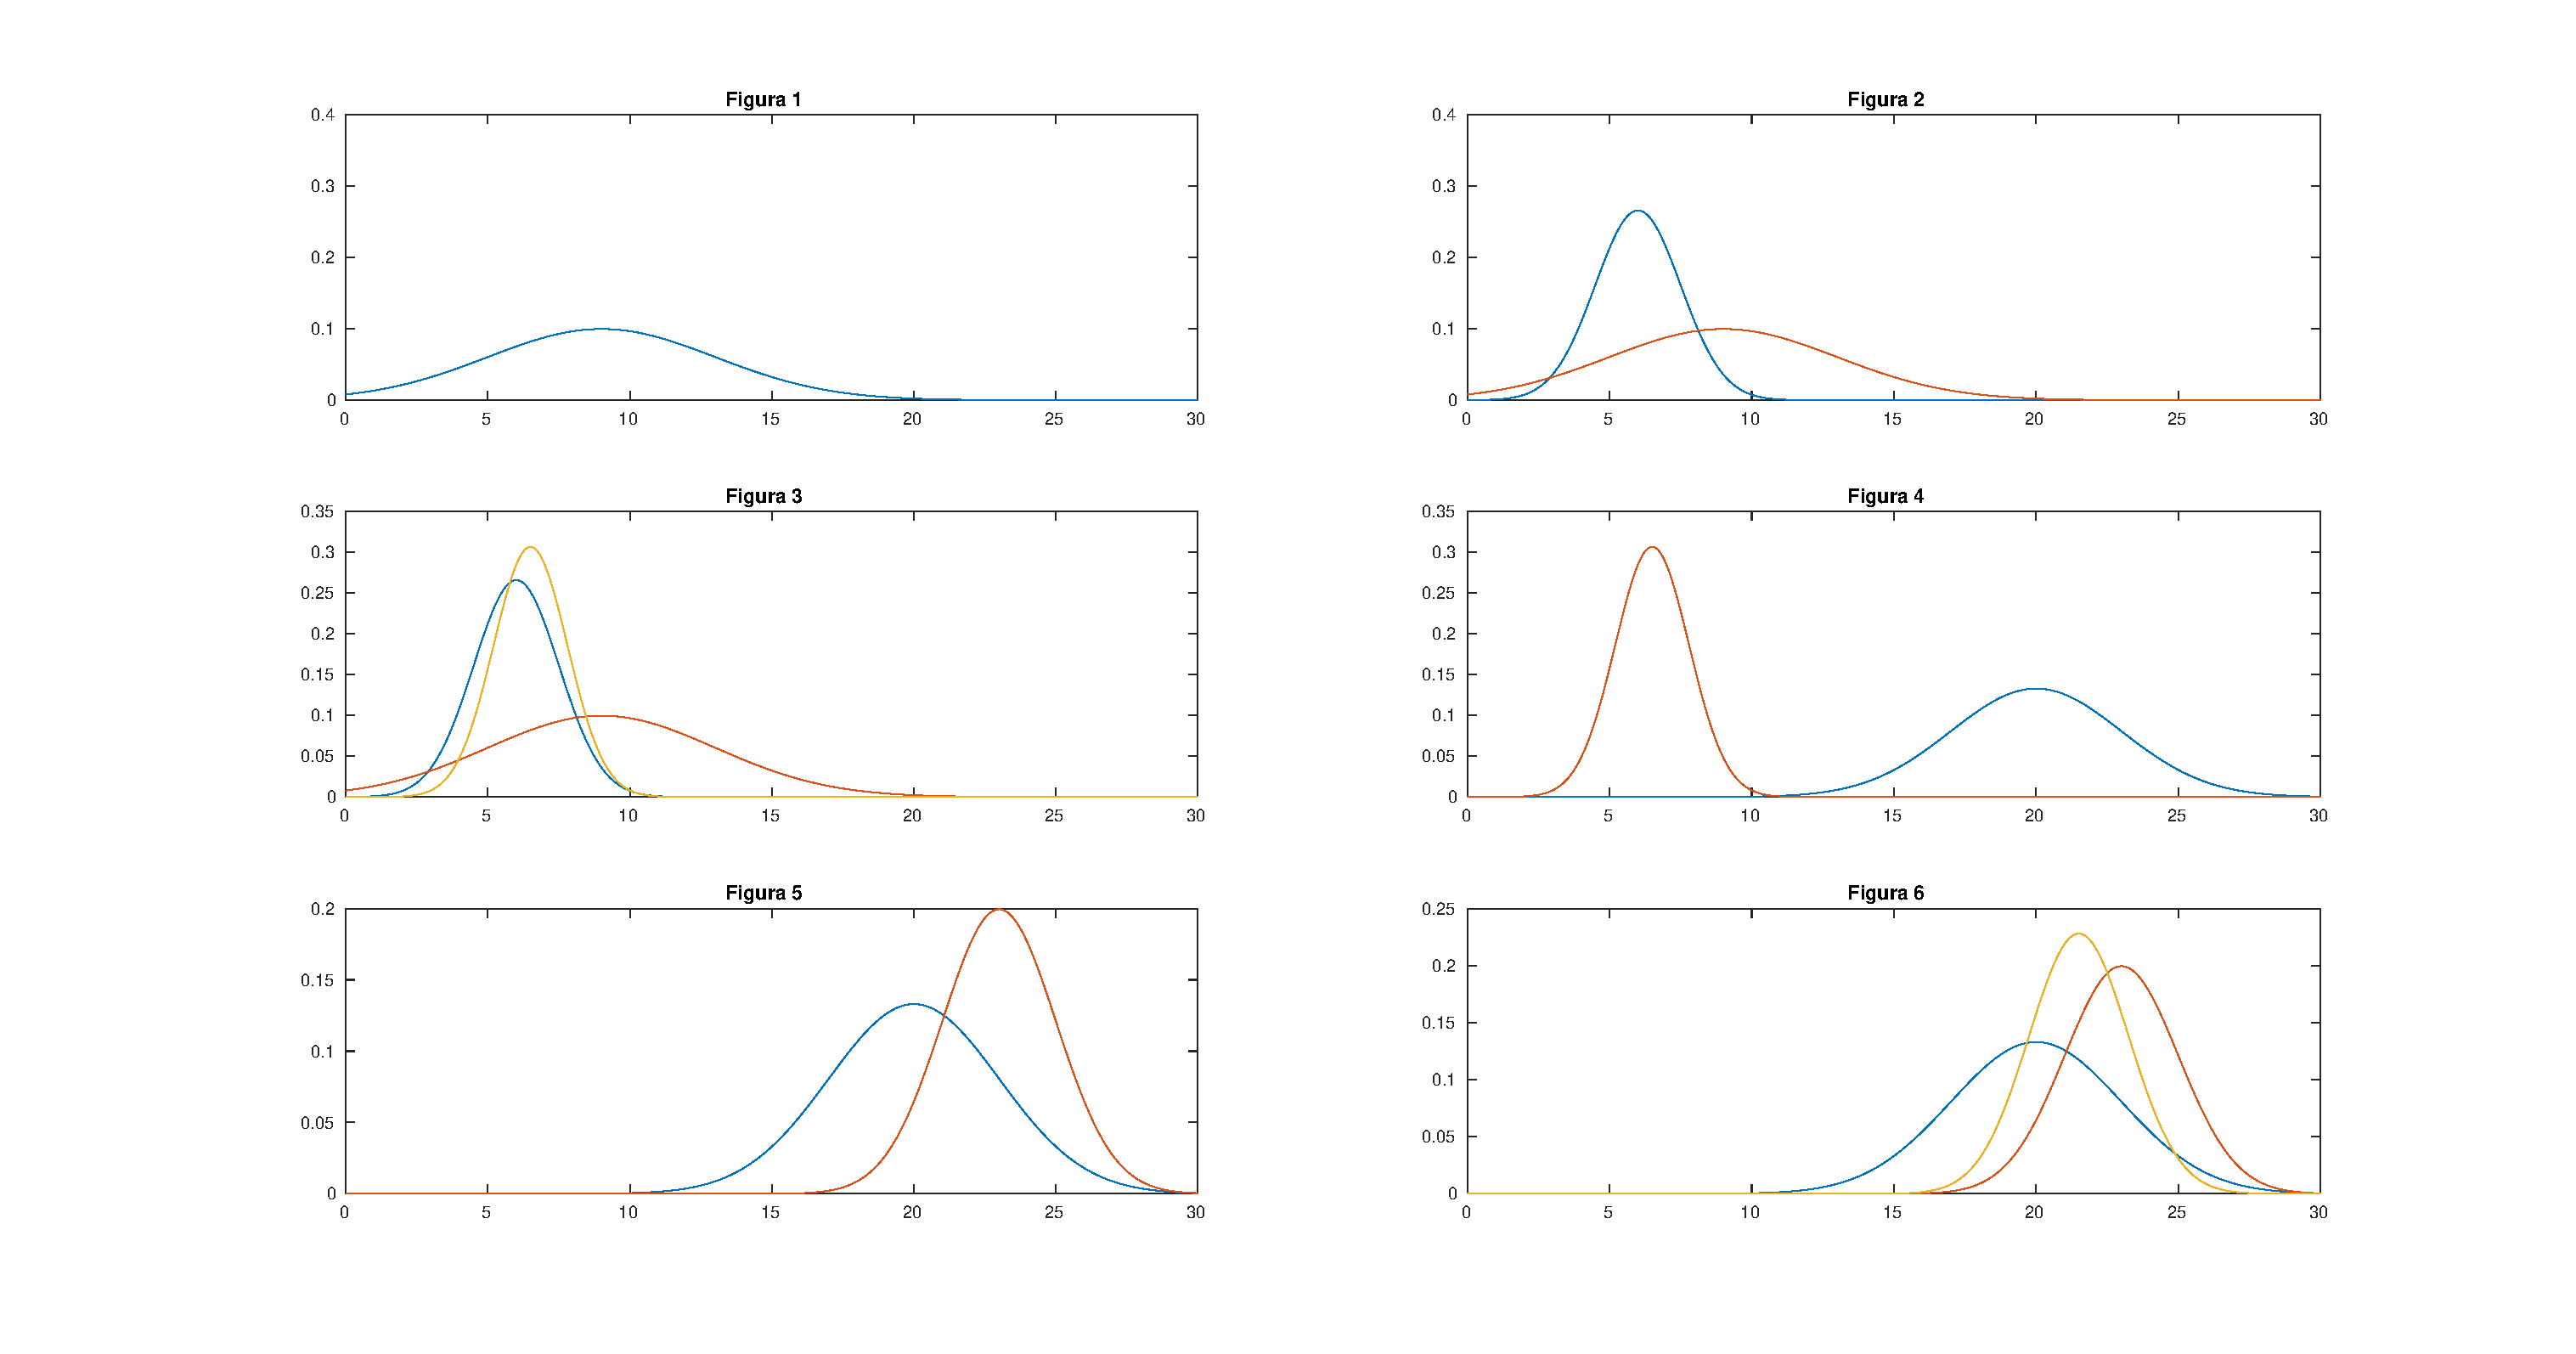
\includegraphics[scale=0.28]{Demostracion-KF}
\caption{Funcionamiento del KF \cite{thrun_probabilistic_2005}.} \label{Demostracion_KF}
\end{figure}

En la figura \ref{Demostracion_KF} muestra un ejemplo simple sobre el funcionamiento del filtro en un espacio unidimensional.
Suponemos que el robot realizará movimientos hacia la derecha en el eje $x$.
La probabilidad a priori de la localización del robot se muestra en la subfigura 1, donde podemos apreciar que la hemos caracterizado siguiendo una distribución Gaussiana.
El robot realizará las medidas del entorno por medio de sus sensores (telémetro, ultrasonidos, etc), y estos devolverán una medida representada mediante otra Gaussiana cuya media será el valor de medida como podemos ver en la subfigura 2.
La Gaussiana de la medida tiene el valor de pico centrado en el devuelto por los sensores, en cuanto a la varianza, esta corresponde a la incertidumbre existente en dicha medida.
Combinando la probabilidad a priori con la medida obtenemos la probabilidad a posteriori que podemos ver en la subfigura 3.
Podemos ver que la certidumbre resultante se encuentra entre las dos medias originales, y la incertidumbre que tiene la nueva Gaussiana es menor que el de las dos Gaussianas anteriores.
El hecho de que las incertidumbre de la Gaussiana resultante sea menor que el de las anteriores puede parecer poco intuitivo.
Este hecho es característico de la integración de la información en el filtro de Kalman donde en general cuanta más información tenemos disponible menos incertidumbre tendremos.

Siguiendo con el ejemplo, ahora suponemos que el robot realiza un movimiento hacia la derecha.
En la subfigura 4 podemos ver como la incertidumbre ha aumentado además de que se ha desplazado en la misma medida que el robot lo ha hecho en el eje hacia la derecha.
En la subfigura 5 el robot vuelve a realizar una medida, que combinada con la probabilidad a priori da como resultado una nueva certidumbre que se muestra en la subfigura 6.
El filtro de Kalman alterna entre el \textit{ciclo de actualización} donde integra las medidas tomadas por lo sensores con el \textit{ciclo de predicción} que modifica la certidumbre conforme a las acciones que ha realizado el robot.
El \textit{ciclo de actualización} reduce la incertidumbre y el \textit{ciclo de predicción} por lo general la aumenta.

\section{Filtro extendido de Kalman (EKF)}
La suposición de que los sistemas tienen transiciones lineales entre estados y que las medidas también son lineales afectadas con ruido Gaussiano aditivo raramente se cumple en la práctica \cite{thrun_probabilistic_2005}.
Un claro ejemplo de la afirmación anterior sería un robot que se mueve con velocidad lineal y angular constante describiendo una trayectoria circular, esta transición de estados no podría ser descrita por ningún tipo de función lineal.
Esta suposición, junto con la suposición de que la certidumbre sigue una distribución unimodal , hace que el KF sea una aproximación demasiado simple, por lo que sería aplicable solamente a problemas triviales de robótica siendo inaplicable en el resto de casos.

El \ac{EKF} supera al \ac{KF} en cuanto a uno de sus supuestos básicos, la linealidad.
En el \ac{EKF} la transición entre estados y las medidas están descritas por funciones no lineales, las funciones $g$ y $h$ respectivamente \cite{thrun_probabilistic_2005}:
\begin{equation}\label{Ec:Estados_EKF}
x_{t}= g(u_{t},x_{t-1})+ \varepsilon_{t}
\end{equation}
\begin{equation}\label{Ec:Medida_EKF}
z_{t}= h(x_{t}) + \delta_{t}
\end{equation}
Este modelo estrictamente generaliza el modelo lineal Gaussiano en el que se basa el \ac{KF}, este modelo lo podemos ver en las ecuaciones \ref{KF_prop_1} y \ref{Ec:medida}.
La función $g$ 
remplaza las matrices $A_{t}$ y $B_{t}$ de la ecuación \ref{KF_prop_1}, y $h$ reemplaza la matriz $C_{t}$ en la ecuación \ref{Ec:medida}.
La evolución de los estados al usar matrices $g$ y $h$ seleccionadas arbitrariamente no presentan una certidumbre distribuida siguiendo una Normal como si ocurría en el \ac{KF}.
De hecho, la realización de la actualización de la certidumbre es normalmente imposible de desarrollar para funciones no lineales $g$ y $h$, ya que los filtros Bayesianos no tienen un método para efectuar este cálculo.
% * <amorellg@ull.edu.es> 2016-06-01T18:10:04.407Z:
%
% > De hecho, la realización de la actualización de la certidumbre es normalmente imposible de realizar para funciones no lineales $g$ y $h$, ya que los filtros Bayesianos no tienen un método para la realización de este cálculo.
%
% "realizar" 3 veces en la misma frase, molaría poner sinónimos
%
% ^ <alu0100765755@ull.edu.es> 2016-06-02T10:57:07.175Z:
%
% Hecho !
%
% ^ <alu0100765755@ull.edu.es> 2016-06-02T11:06:00.540Z.

El \ac{EKF} calcula una aproximación a la certidumbre real por medio de una distribución Gaussiana.
En particular, la certidumbre $bel(x_{t})$ en un tiempo $t$ es representada por una media $\mu_{t}$ y una covarianza $\Sigma_{t}$ como ya explicamos en el capítulo \ref{ch:capitulo2}.
Así el \ac{EKF} hereda del \ac{KF} la forma de representar la certidumbre, pero se diferencia en que esta será una mera aproximación y no es calculada como en el \ac{KF}.

\subsection{Linealización mediante la expansión de Taylor }

Como ya hemos dicho uno de los puntos básicos del \ac{EKF} es la representación de la certidumbre mediante una aproximación de esta.
Por lo tanto la idea principal es la \textit{linealización}.
Si suponemos que tenemos una función no lineal $g$ una función Gaussiana proyectada a través de esta función se convertirá en no Gaussiana.
Esto es porque existen no linealidades en $g$ que perturban la certidumbre de tal manera que hacen que no puede ajustarse a una Gaussiana.
Por lo tanto con la linealización lo que buscamos es aproximar la función $g$ con una función lineal que sea tangente a la función $g$ en la media de la Gaussiana.
Proyectando la Gaussiana por medio de esta aproximación lineal, la distribución de probabilidad a posteriori si será una Gaussiana.
% * <amorellg@ull.edu.es> 2016-06-01T18:11:54.614Z:
%
% > posterior
%
% otras veces te has referido como "a posteriori", usar "posterior" igual puede llevar a confusión
%
% ^ <alu0100765755@ull.edu.es> 2016-06-02T11:06:16.671Z.
De hecho, una vez que $g$ ha sido linealizada el método para la propagación de la certidumbre es igual que para el \ac{KF}.
La misma explicación se aplica a la multiplicación de Gaussianas cuando se utiliza la función $h$.
Para este caso el \ac{EKF} vuelve a aproximar la función $h$ por medio de una función lineal que es tangente a $h$, manteniendo así la naturaleza Gaussiana de la probabilidad a posteriori.

A la hora de linealizar funciones no lineales pueden utilizarse una gran variedad de técnicas.
En concreto el \ac{EKF} utiliza un método llamado \textbf{expansión de Taylor} \cite{_taylor_2016}.
En el \ac{EKF} se suelen trabajar con expansiones de primer y segundo orden.
La expansión de Taylor constituye una aproximación lineal a una función g por medio del valor de sus derivadas y su pendiente.
La pendiente viene dada por la derivada parcial siguiente:
\begin{equation}\label{Ec:Taylor_1}
g'(u_{t},x_{t-1}) := \frac{\partial g(u_{t},x_{t-1})}{\partial x_{t-1}}
\end{equation}
Está claro que el valor de g y su pendiente dependerá de los argumentos de $g$ (vector de estados y de control).
Una elección lógica para seleccionar los argumentos es elegir el estado que se considera más probable en el instante en el que se realiza la linealización.
Para las distribuciones Gaussianas, el estado más probable es la media del posterior estado de control $u_{t-1}$.
En otras palabras, $g$ es aproximada por su valor en el instante en que se da $u_{t-1}$ (y $u_t$).
La linealización por tanto se conseguiría de la siguiente forma:
\begin{equation}\label{Ec:Taylor_2}
g(u_{t},x_{t-1}) \approx g(u_{t},\mu_{t-1}) + g'(u_{t},\mu_{t-1})(x_{t-1}-\mu_{t-1}) 
= g(u_{t},\mu_{t-1}) + G_{t}(x_{t-1}-\mu_{t-1})
\end{equation}
Si lo escribimos utilizando la expresión de una Gaussiana tendríamos:
\begin{eqnarray}\label{Ec:Prob_Taylor}
\nonumber p(x_{t} \mid u_{t},x_{t-1}) \approx \\
\nonumber det(2\pi R_{t})^{-\frac{1}{2}}exp(-\frac{1}{2}[x_{t}-g(u_{t},\mu_{t-1})-G_{t}(x_{t-1}-\mu_{t-1})]^{T} \\
R_{t}^{-1}[x_{t}-g(u_{t},\mu_{t-1})-G_{t}(x_{t-1}-\mu_{t-1})])
\end{eqnarray}
La matriz $G_{t}$ es una matriz de dimensiones $nxn$, donde $n$ es la dimensión del vector de estados.
Esta matriz se conoce con el nombre de \textbf{Jacobiano}.
El valor del Jacobiano depende de $u_{t}$ y $u_{t-1}$, por lo tanto se diferencia para distintos instantes de tiempo.

La misma linealización es implementada para la función de medida $h$.
En esta expresión la serie de Taylor se desarrolla alrededor de $\bar{\mu_{t}}$, que es el estado que se considera más probable para linealizar la función de la siguiente manera:
\begin{eqnarray}\label{Ec:Prob_Taylor_h}
\nonumber h(x_{t}) \approx h(\bar{\mu_{t}}) + h'(\bar{\mu_{t}})(x_{t}-\bar{\mu_{t}}) \\
= h(\bar{\mu_{t}}) + H_{t}(x_{t}- \bar{\mu_{t}}) 
\end{eqnarray}
Sabiendo que $h'(x_{t})=\frac{\partial h(x_{t}}{\partial x_{t}}$ podemos escribir la expresión en forma de Gaussiana:
\begin{eqnarray}\label{Ec:Prob_Taylor_h_Gauss}
\nonumber p(z_{t} \mid x_{t}) = det(2\pi Q_{t})^\frac{-1}{2} exp(-\frac{-1}{2}[z_{t}-h(\bar{\mu_{t}})-H_{t}(x_{t}-\bar{\mu_{t}}]^{T} \\
Q_{T}^{-1}[z_{t}-h(\bar{\mu_{t}})-H_{t}(x_{t}-\bar{\mu_{t}})])
\end{eqnarray}

De esta manera aplicariamos los desarrollos de Taylor en el \ac{EKF} y podríamos seguir usando los supuestos de que las certidumbres vienen dadas por distribuciones Gaussianas.

\subsection{Algortimo del EKF}
\begin{figure}[ht!]
\centering
\includegraphics[scale=0.87]{Alg_EKF}
\caption{Iteración del EKF \cite{leonardo_navegacion_2011} \cite{AnIntroductionToTheKalmanFilter}.} \label{Iteracion_EKF}
\end{figure}
\begin{algorithm}
\begin{algorithmic} 
\STATE{$\bar{\mu_{t}}= g(u_{t},\mu_{t-1}) $}
\STATE{$\bar{\Sigma_{t}}=G_{t}\Sigma_{t-1}G_{t}^{T}+R_{t}$}
\STATE{$K_{t}=\bar{\Sigma_{t}}H_{t}^{T}(H_{t}\bar{\Sigma_{t}}H_{t}^{T}+Q_{t})^{-1}$}
\STATE{$\mu_{t}= \bar{\mu_{t}}+K_{t}(z_{t}-h(\bar{\mu_{t}}))$}
\STATE {$\Sigma_{t} = (I-K_{t}H_{t})\bar{\Sigma_{t}}$}
\RETURN $\mu_{t},\Sigma_{t}$
\end{algorithmic}
\caption{Algoritmo EKF \cite{thrun_probabilistic_2005} $(\mu_{t-1},\Sigma_{t-1},u_{t},z_{t})$}\label{alg:algoritmoEKF}
\end{algorithm}

En el algoritmo \ref{alg:algoritmoEKF} y la figura \ref{Iteracion_EKF} podemos ver las ecuaciones que usa el \ac{EKF} para funcionar.
Como podemos apreciar este algoritmo es muy parecido al algortimo \ref{alg:algoritmoKF} donde se aplicaba el \ac{KF}.
Las diferencias más importantes las podemos apreciar en las líneas 1 y 4 en ambos algoritmos.
La predicción del estado (línea 1) en el \ac{KF} se realiza de la forma $A_{t}\mu_{t-1}+ B_{t}\mu_{t}$ mientras que en el \ac{EKF} se realiza de la forma $g(u_{t},\mu_{t-1})$ por lo tanto la predicción de los estados se calculan de forma diferente.
Por otra parte también se diferencian en la predicción de la medida (línea 4) en el \ac{KF} se expresa como $C_{t}\bar{\mu_{t}}$ mientras que en el \ac{EKF} se define como $h(\bar{\mu_{t}})$.

Podemos ver que la predicción lineal usada en el \ac{KF} ha sido reemplazada por expresiones no lineales en el \ac{EKF}.
Además, el filtro extendido de Kalman usa los Jacobianos $G_{t}$ y $H_{t}$ en lugar de las matrices lineales $A_{t}$,$B_{t}$ y $C_{t}$ presentes en el filtro clásico de Kalman.
El Jacobiano $G_{t}$ en el \ac{EKF} corresponde a las matrices $A_{t}$ y $B_{t}$ del \ac{KF}, por otro lado el Hessiano $H_{t}$ corresponde a la matriz $C_{t}$.

\section{ Filtro \textit{unscented} de Kalman (UKF)}
El filtro \ac{UKF} es una formulación para sistemas no lineales \cite{julier_new_2000} al igual que el \ac{EKF} pero sin utilizar la forma de linealizar el sistema de este último.
La diferencia básica está en la manera en la que las variables aleatorias Gaussianas que modelan el ruido son representadas y propagadas a través de la dinámica del sistema.
El \ac{UKF} resuelve este problema por medio de un muestreo determinista.
El \ac{UKF} mantiene la estructura de predicción-corrección tanto del \ac{KF} como del \ac{EKF} que podemos ver en las figuras \ref{Iteracion_KF} y \ref{Iteracion_EKF} pero la forma de realizar el cálculo es diferente.
En lugar de estimar la covarianza del error $\Sigma_{k}^{-}$ utilizando el procedimiento del \ac{EKF}, se hace uso de lo que se conoce como transformación Unscented (UT) \cite{julier_new_2000} que calcula un conjunto de puntos de muestra, conocidos como \textbf{puntos Sigma}, para representar de forma más precisa la media y la varianza del estado ( suponiendo que esta tiene una distribución Gaussiana).
Si propagamos estos puntos a través del sistema no lineal de las ecuaciones \ref{Ec:Estados_EKF} y \ref{Ec:Medida_EKF} la media y la covarianza posterior se obtiene para cualquier no-linealidad presente en el sistema de forma precisa, dando un mejor resultado si lo comparamos con la linealización realizada en el \ac{EKF} tal y como podemos ver en la figura \ref{EKF_UKF_UT}   \cite{julier_general_1996} \cite{julier_new_1995} \cite{julier_unscented_2004}.
Los valores de los puntos sigma (que son escogidos cuidadosamente) se utilizan para obtener la predicción del estado y de su covarianza en una estimación \textit{a priori}.
El \ac{UKF} se postula como un filtro muy preciso en cuanto a la estimación de estados (se trataría de una aproximación de segundo orden), sin embargo, es muy costoso en términos de potencia de cálculo necesaria ya que el algortimo de este filtro necesita calcular la raíz cuadrada de la matriz $\Sigma_{k}^{-}$ aunque por otra parte no es necesario el cálculo del Jacobiano ni del Hessiano.
El \ac{UKF} no podría ser implementado en robots con recursos limitados ya que para estos llevaría mucho tiempo tratar de calcular la operación anterior.

\begin{figure}[ht!]
\centering
\includegraphics[scale=0.95]{EKF_UT}
\caption{Comparativa linealización y transformada UT \cite{leonardo_navegacion_2011} \cite{wan_unscented_2000} .} \label{EKF_UKF_UT}
\end{figure}

\subsection{La transformación \textit{unscented} (UT)}

La predicción de los estados futuros de un sistema puede calcularse de distintas formas, la transformada UT es uno de ellas.
Suponiendo que $x$ es un variable aleatoria con media $\mu_{x}$ y covarianza $\Sigma_{x}$ una segunda variable aleatoria $y$ se podría relacionar con $x$ por medio de la función no lineal:
\begin{equation}\label{Ec:Trans_UT_1}
y = f(x)
\end{equation}
A la función anterior le podemos calcular a su vez la media ($\mu_{y}$) y la covarianza ($\Sigma_{y}$).
Los distribución de probabilidad de la variable transformada es consistente si se satisface la desigualdad \cite{_leyton_2009} \cite{julier_unscented_2004} en términos de la covarianza y la media de la expresión siguiente:
\begin{equation}\label{Ec:Trans_UT_2}
\Sigma_{y}- E[(y-\mu_{y})(y-\mu_{y})^{T}] \ge 0
\end{equation}
Si no se cumple la condición \ref{Ec:Trans_UT_2} se podrá considerar a $\Sigma_{y}$ subestimada.
Sin embargo, la consistencia no necesariamente implica que vayamos a obtener buenos resultados ya que los cálculos finales están sujetos a la minimización del error cuadrático medio.

La transformada \textit{unscented} es un novedoso método utilizado para calcular la distribución de probabilidad de una variable aleatoria que ha sido sometida a una transformación no lineal.
Este método se basa en la idea de que es más fácil aproximar una distribución Gaussiana que aproximar una función no lineal arbitraria \cite{julier_new_1995}. 
El método consiste en elegir un conjunto de puntos llamados \textbf{puntos sigma}, con la condición de que su media y covarianza coincida con las de la variable aleatoria $x$ del proceso.
A continuación, la transformación no-lineal $f$ se aplica a cada punto sigma y a estos puntos $(y=f(x))$ se les calcula la esperanza $E[y]$ y la covarianza $\Sigma_{y}$.

Si $x$ es una variable aleatoria de dimensión $L$ con media $E[x] = \mu_{x}$ y covarianza $\Sigma_{x}$, entonces para calcular la media $E[y]=\mu_{y}$ y la covarianza $P(y) = \Sigma_{y}$ se construye la matriz de puntos sigma $\chi_{0}$ con $(2L+1)$ vectores columna \cite{houshangi_accurate_2005} \cite{chow_unscented_2007} resultando:

\begin{eqnarray}\label{Ec:Chi_UKF_UT}
\nonumber \chi_{0} = \mu_{x} \\
\nonumber \chi_{i} = \mu_{x} + (\sqrt[]{(L+ \lambda)\Sigma_{x}})_{i} ; i=1,\cdots,L \\
\chi_{i} = \mu_{x} - (\sqrt[]{(L+ \lambda)\Sigma_{x}})_{i-L} ; i=L+1,\cdots,2L 
\end{eqnarray}
donde $\delta = \alpha^{2}(L+k)-L$ y $\alpha$ (generalmente $1x10^{-4} \le \alpha \le 1 $) determinan la dispersión de los puntos alrededor de $\mu_{x}$, $k$ es una constante relacionada con el parámetro de escala (generalmente $0 \le k \le 3-L$) y $(\sqrt[]{(L+ \delta)\Sigma_{x}})$ es la i-ésima columna de la matriz cuadrada $(L+ \delta)\Sigma_{x}$.

El cálculo de la media y la covarianza de la variable aleatoria también se puede lograr mediante la utilización de una descomposición de Cholesky \cite{oh_development_2006} \cite{_leyton_2009} y será en definitiva la que se utilizará para la implementación que se realiza en la toolbox \cite{toolbox_simo} del \ac{UKF}.

Se puede comprobar que los puntos sigma contienen la media y la covarianza de $x$ en las siguientes ecuaciones que describen en forma simplificada la idea final del método propuesto para el \ac{UKF} \cite{julier_unscented_2004}:
\begin{equation}\label{Ec:Trans_UT_3}
\mu^{(UT)} \equiv \sum_{i=0}^{2L} W_{i}^{(m)}\chi_{i}= \mu_{x}
\end{equation}
\begin{equation}\label{Ec:Trans_UT_4}
\Sigma_{x}^{(UT)} \equiv \sum_{i=0}^{2L} W_{i}^{(c)}(\chi_{i}-\mu_{x}^{(UT)})(\chi_{i}-\mu_{x}^{(UT)})^{T} = \Sigma_{x}
\end{equation}
Donde los términos $W_{i}^{(c)}$ y $W_{i}^{(m)}$ son escalares que asignan un peso estadístico a la medida y dependen de los parámetros $\alpha ,k y \beta$ como se plantea en las ecuaciones \ref{Ec:Trans_UT_5}.
Los valores de los parámetros son determinados según el tipo de dispersión y la distribución de probabilidad propuesta en el desarrollo de cada modelo.
Los pesos estadísticos $W_{i}^{(c)}$ y $W_{i}^{(m)}$ se definen de la siguiente manera:
\begin{eqnarray}\label{Ec:Trans_UT_5}
\nonumber W_{0}^{(m)}= \frac{\lambda}{L+\lambda} \\
\nonumber W_{0}^{(c)}= \frac{\lambda}{L+\lambda} + 1-\alpha^{2}+\beta  \\
W_{i}^{(m)} = W_{i}^{(c)} = \frac{1}{2(L+\lambda)} ; i=1,\cdots,2L
\end{eqnarray}
donde $\beta$ es el parámetro que incorpora el conocimiento que se tiene de antemano acerca de la distribución $x$(generalmente $\beta=2$ cuando se trata de distribuciones Gaussianas).
Ahora, la transformación no-lineal $f$ se aplica a cada conjunto de puntos sigma con el fin de generar una nube de puntos transformados (ecuación \ref{Ec:Trans_UT_6}) y de su distribución de probabilidad estimaremos la media:
\begin{equation}\label{Ec:Trans_UT_6}
Y_{i} = f(\chi_{i}); i=0,\cdots,2L
\end{equation}
\begin{equation}\label{Ec:Trans_UT_7}
\mu_{y} \approx \mu_{y}^{(UT)} = \sum_{i=0}^{2L}W_{i}^{(m)}Y_{i}
\end{equation}
La covarianza, se determina de la siguiente manera:
\begin{equation}\label{Ec:Trans_UT_8}
\Sigma_{y} \approx \Sigma_{y}^{(UT)} = \sum_{i=0}^{2L} W_{i}^{(c)}(Y_{i}-\mu_{y}^{(UT)})(Y_{i}-\mu_{y}^{(UT)})^{T}
\end{equation}
\subsection{Algoritmo del UKF}
Una vez entendemos el principio funcionamiento de la transformada UT podemos pasar a explicar el algoritmo completo del \ac{UKF}.
El \ac{UKF} puede considerarse el resultado de de incorporar esta transformación al \ac{EKF} \cite{_leyton_2009}.
Lo que intenta el \ac{UKF} es mejorar las aproximaciones que se hacen de los dos primeros momentos de una variable aleatoria que resulta de propagar otra variable aleatoria tomada como Gaussiana a través de la transformada \textit{unscented}.

En el algortimo \ref{alg:algoritmoUKF} podemos ver como funciona este filtro, además en la figura \ref{Iteracion_UKF} podemos ver el ciclo realizado durante el funcionamiento del filtro.
El algoritmo \ref{alg:algoritmoUKF} corresponde a lo que se conoce como la versión \textit{NonAugmented} del filtro \ac{UKF} que es aplicada a sistemas afectados con ruido aditivo de media cero, además es una de las versiones con la implementación más sencilla.

Para la aplicación del algortimo hay que tener en cuenta que debemos establecer unos valores iniciales para $\hat{x}_{0}$ y $\Sigma_{0}$, los valores son los siguientes:
\begin{equation}\label{Ec:Trans_UT_9}
\hat{x}_{0} = E[x_{0}]
\end{equation}
\begin{equation}\label{Ec:Trans_UT_10}
\Sigma_{0} = E[(x_{0}-\hat{x}_{0})(x_{0}-\hat{x}_{0})^{T}]
\end{equation}

\begin{figure}[ht!]
\centering
\includegraphics[scale=1.95]{Alg_UKF}
\caption{Iteración UKF \cite{_leyton_2009} \cite{luigi_d&39;alfonso_mobile_2015} .} \label{Iteracion_UKF}
\end{figure}
La idea de este algoritmo es muy parecida a la presentada para el \ac{EKF} con la única diferencia de cómo se propaga la media y la covarianza a través del sistema.
La figura \ref{EKF_UKF_UT} ilustra con un ejemplo sencillo las diferentes formas de propagación de la media y la covarianza para un sistema de dos dimensiones.
En el lado izquierdo se observan la media y la covarianza verdaderas usando el muestreo de Monte Carlo.
En el centro de la figura se muestra el resultado si usaramos la linealización del \ac{EKF}.
Por último, podemos ver el resultado de la transformada \textit{unscented} y como vemos únicamente nos hacen falta 5 puntos para tener una propagación con una media y covarianza representativa.
Si tenemos en cuenta las ideas anteriores podemos ver las similitudes en los algortimos \ref{alg:algoritmoEKF} y \ref{alg:algoritmoUKF} \cite{zhou_ukf_2007}.
\begin{algorithm}
\begin{algorithmic} 
\STATE{$B_{t} = \sqrt[]{(n+\lambda)\Sigma_{t}} $}
\STATE{$\chi_{t} = [\hat{x_{t}}\hat{x_{t}} + B_{t}\hat{x_{t}}-B_{t}]$}
\STATE{$\chi_{t+1}^{*}=f(\chi_{t},u_{t})$}
\STATE{$\hat{x}_{t+1}= \chi_{t+1}^{*}R^{m}$}
\STATE {$\Sigma_{t+1} = (\chi_{t+1}^{*}-\hat{x}_{t+1})R^{C}(\chi_{t+1}^{*}-\hat{x}_{t+1})'+ W_{k} $}
\STATE{$B_{t+1}= \sqrt[]{(n+\lambda)\Sigma_{t+1}}$}
\STATE{$\chi_{t+1} = [\hat{x}_{t+1}\hat{x}_{t+1}+ B_{t+1}\hat{x}_{t+1}-B_{t+1}]$}
\STATE{$\Gamma_{t+1}=h(\chi_{t+1})$}
\STATE{$\hat{y}_{t+1}=\Gamma_{t+1}R^{m}$}
\STATE{$\Sigma_{yy}=(\Gamma_{t+1}-\hat{y}_{t+1})R^{C}(\Gamma_{t+1}-\hat{y}_{t+1})' + V$}
\STATE{$\Sigma_{xy}=(\chi_{t+1}-\hat{x}_{t+1})R^{C}(\Gamma_{t+1}-\hat{y}_{t+1})'$}
\STATE{$K_{t+1}=\Sigma_{xy}\Sigma_{yy}^{-1}$}
\STATE{$\hat{x}_{t+1}^{+}=\hat{x}_{t+1}+K_{t+1}(y_{t+1}-\hat{y}_{t+1})$}
\STATE{$\Sigma_{t+1}^{+} = \Sigma_{t+1}- K_{t+1}\Sigma_{yy}K_{t+1}^{'} $}
\RETURN $\hat{x}_{t+1}^{+},\Sigma_{t+1}^{+}$
\end{algorithmic}
\caption{Algoritmo UKF \cite{_leyton_2009} \cite{luigi_d&39;alfonso_mobile_2015}}\label{alg:algoritmoUKF}
\end{algorithm}

\section{Filtro de Kalman de Cubatura (CKF)}
Cuando afrontamos la estimación de estados en sistemas no lineales, tenemos que dejar de lado la idea de buscar una solución óptima o analítica y debemos conformarnos con una solución subóptima dada por los filtros Bayesianos \cite{_cubature-based_2010} \cite{ienkaran_cubature_2009} \cite{zhang_cubature_2013}.
En términos computacionales una solución subóptima para la densidad de probabilidad a posteriori puede ser obtenida usando una de las siguientes aproximaciones:
\begin{itemize}
\item \textbf{Aproximación local}: En este tipo de aproximación derivamos los filtros no lineales para que la distribución de probabilidad a posteriori tome la forma de la distribución a priori.
Por ejemplo, podemos asumir que se sigue una distribución Gaussiana como hemos hecho en los anteriores filtros (\ac{EKF} y \ac{UKF}).
Este tipo de aproximaciones generan filtros más simples y de una ejecución más rápida.
\item \textbf{Aproximación global}: Aquí no realizamos ningún tipo de suposición específica acerca de la densidad de probabilidad a posteriori. 
Por ejemplo, los filtros de partículas usando integraciones de Monte Carlo con el \textit{sampling importance resampling (SIR)} entra dentro de esta aproximación.
% * <amorellg@ull.edu.es> 2016-06-01T18:28:47.025Z:
%
% > muestro de importancia
%
% esto no lo dejes así literal, ponlo en castellano (en cursiva por ejemplo) y mejor referirse por el original inglés, sampling importance resampling (SIR), me suena raro verlo así traducido vaya :P
%
% ^ <alu0100765755@ull.edu.es> 2016-06-02T11:08:38.922Z.
Normalmente lo métodos globales requieren una gran cantidad de recursos computacionales.
\end{itemize}
Desafortunadamente, los filtros para sistemas no lineales que hemos visto sufren el problema de lo que se conoce como \textit{maldición de la dimensionalidad} además de la \textit{divergencia} \cite{ienkaran_cubature_2009}.
Este efecto puede causar que el filtro vea degradado su rendimiento computacional cuando trabajamos con modelos con una alta dimensión de estados, normalmente con vectores con dimensión superior a 20 estados.
% * <amorellg@ull.edu.es> 2016-06-01T18:31:00.806Z:
%
% > entre en detrimento
%
% mejor "vea degradado su rendimiento computacional"
%
% ^ <alu0100765755@ull.edu.es> 2016-06-02T11:09:51.042Z.
La divergencia puede ocurrir por muchas razones, como podrían ser la imprecisión, un modelo incompleto de nuestro sistema físico o incluso la pérdida de información al capturar la verdadera distribución de probabilidad a posteriori.
Por ejemplo, el \ac{EKF}, que es uno de los filtros más utilizados para sistemas no lineales desde hace décadas trabaja bien en algunas aplicaciones de filtrado que no presenten grandes no linealidades, en caso contrario el sistema presentaría divergencias y el filtro no funcionaría correctamente.

Con la motivación de solucionar el problema anterior surgió lo que se conoce como Filtro de Kalman de Cubatura (CKF).
Como sabemos los filtros Bayesianos son muy fáciles de manejar cuando se asume que todas las densidades de probabilidad son Gaussianas.
De ser así el problema se reduce a calcular integrales multidimensionales cuyos integrandos son de la forma $función no lineal x Gaussiana$.
El \ac{CKF} aprovecha lo que se conoce como las \textit{reglas de cubatura} que sirven para realizar integrales multidimensionales con alta eficiencia de computo.
Con las reglas de cubatura a nuestra disposición podemos describir el funcionamiento del filtro como el filtrado no lineal a través de la teoría estimación lineal, gracias a esta regla de integración el filtro posee su nombre.
El \ac{CKF} se presenta como un filtro numéricamente muy preciso y además fácilmente extensible a problemas de estimación de gran número de dimensiones.

En cuanto a la base matemática el \ac{CKF} presenta muchas similitudes con el \ac{UKF} aunque su ámbito de aplicación es ligeramente distinto.
Ambos métodos usan puntos seleccionados de forma determinista para caracterizar las distribuciones de probabilidad aunque como podremos imaginar estos se hallan de distinta manera para cada filtro.
Recordemos que para el \ac{UKF} seleccionábamos $(2n+1)$ puntos de muestreo con pesos $[\chi_{i},\omega_{i}]_{i=0}^{2n}$ para caracterizar nuestra distribución de probabilidad, siendo $n$ la dimensión del vector de estados.
Para el \ac{CKF} utilizaremos $2n$ puntos para caracterizar nuestra distribución de probabilidad.


\subsection{Transformación esférica-radial}
Como hemos dicho en la sección anterior, el filtrado de sistemas no lineales usando la suposición de distribuciones Gaussianas reduce el problema a cómo calcular las integrales cuyos integrandos son de la forma $función no lineal x Gaussiana$.
Específicamente consideraremos la integral de la siguiente forma:
\begin{equation}\label{Ec:CKF_1}
I(f)=\int_{R^{n}}f(x)exp(-x^{T}x)dx 
\end{equation}
Definida en el sistema cartesiano de coordenadas.
Para calcular el valor numérico de dicha integral lo que haremos será transformarla en la forma esférica-radial, y posteriormente se usará una regla esférica-radial de tercer grado.

En la transformación esférica-radial, el paso clave es cambiar el sistema de coordenadas cartesiano (vector $x$) a un sistema con radio $r$ y vector director $y$.
La transformación sería $x=ry$ donde $y^{T}y=1$, por lo tanto $x^{T}x=r^{2}$.
De esta manera la integral \ref{Ec:CKF_1} puede ser reescrita en el sistema de coordenadas esférico-radial como:
\begin{equation}\label{Ec:CKF_2}
I(f)=\int_{0}^{\infty}\int_{U_{n}}f(ry)r^{n-1}exp(-r^{2})d\sigma(y)dr 
\end{equation}
Donde $U_{n}$ es la superficie de la esfera definida por $U_{n}=[y \epsilon R^{n} \mid y^{T}y=1]$ y $\sigma$ es la superficie esférica medida o lo que es lo mismo, el área de $U_{n}$. 
Podemos escribir la integral radial como:
\begin{equation}\label{Ec:CKF_3}
I=\int_{0}^{\infty}S(r)r^{n-1}exp(-r^{2})dr \approx w_{1}f(x_{1})
\end{equation}
donde $S(r)$ es definido por la integral esférica con la función de unidad de peso $w(y)=1$ que puede ser aproximada por $2n$ puntos \cite{zhang_cubature_2013}:
\begin{equation}\label{Ec:CKF_4}
S(r)= \int_{U_{n}}f(ry)d\sigma(y) \approx w\sum_{i=1}^{2n}f[u]_{i}
\end{equation}
Donde $w>0$ es el peso correspondiente para el generador $[u]$, por lo tanto finalmente tendríamos:
\begin{equation}\label{Ec:CKF_5}
I(f)=\int_{R^{n}}f(x)exp(-x^{T}x)dx = \frac{\sqrt[]{\pi^{n}}}{2n}\sum_{i=1}^{2n}f(\sqrt[]{\frac{n}{2}}[1]_{i})
\end{equation}

Estas integrales esféricas y radiales son normalmente calculadas siguiendo lo que se conoce como \textbf{regla esférica de cubatura} y la \textbf{regla Gaussiana de cuadratura} que pueden ser consultadas en \cite{zhang_cubature_2013} \cite{ienkaran_cubature_2009} \cite{_cubature-based_2010}.

\subsection{Algoritmo del CKF}
\begin{algorithm}
\begin{algorithmic} 
\STATE{$P_{k-1\mid k-1} = S_{k-1\mid k-1}S_{k-1\mid k-1}^{T} $}
\STATE{$X_{i,k-1\mid k-1} = S_{k-1\mid k-1}\xi_{i} + \hat{x}_{k-1\mid k-1}$}
\STATE{$X_{i,k\mid k-1}^{*}= f(X_{i,k-1\mid k-1},u_{k-1})$}
\STATE{$\hat{x}_{k\mid k-1}=\frac{1}{m}\sum_{i=1}^{m}X_{i,k\mid k-1}^{*}$}
\STATE{$P_{k\mid k-1} = \frac{1}{m}\sum_{i=1}^{m}X_{i,k\mid k-1}^{*}X_{i,k\mid k-1}^{*T}-\hat{x}_{k\mid k-1}\hat{x}_{k\mid k-1}^{T} + Q_{k-1} $}
\STATE{$P_{k\mid k-1} = S_{k\mid k-1}S_{k\mid k-1}^{T} $}
\STATE{$X_{i,k\mid k-1} = S_{k\mid k-1}\xi_{i} + \hat{x}_{k\mid k-1}$}
\STATE{$Z_{i,k\mid k-1} = h(X_{i,k\mid k-1},u_{k})$}
\STATE{$\hat{z}_{k\mid k-1}=\frac{1}{m}\sum_{i=1}^{m}Z_{i,k\mid k-1}$}
\STATE{$P_{zz,k\mid k-1} = \frac{1}{m}\sum_{i=1}^{m}Z_{i,k\mid k-1}Z_{i,k\mid k-1}^{T}-\hat{z}_{k\mid k-1}\hat{z}_{k\mid k-1}^{T} + R_{k} $}
\STATE{$P_{xz,k\mid k-1} = \sum_{i=1}^{m}w_{i}X_{i,k\mid k-1}Z_{i,k\mid k-1}^{T}-\hat{x}_{k\mid k-1}\hat{z}_{k\mid k-1}^{T}$}
\STATE{$W_{k}=P_{xz,k\mid k-1}P_{zz,k \mid k-1}^{-1}$}
\STATE{$\hat{x}_{k\mid k} = \hat{x}_{k \mid k-1} + W_{k}(z_{k}-\hat{z}_{k\mid k-1})$}
\STATE{$P_{k\mid k} = P_{k\mid k-1} - W_{k}P_{zz,k\mid k-1}W_{k}^{T}$}
\RETURN $\hat{x}_{k\mid k},P_{k\mid k}$
\end{algorithmic}
\caption{Algoritmo CKF \cite{ienkaran_cubature_2009}}\label{alg:algoritmoCKF}
\end{algorithm}

\begin{figure}[ht!]
\centering
\includegraphics[scale=1.65]{Alg_CKF}
\caption{Iteración CKF \cite{ienkaran_cubature_2009}.} \label{Iteracion_CKF}
\end{figure}
En el algoritmo \ref{alg:algoritmoCKF} y la figura \ref{Iteracion_CKF} podemos ver el funcionamiento básico del \ac{CKF}.
Como en todos los filtros que hemos visto se mantiene la estructura predicción-actualización que permite al filtro funcionar de forma iterativa.
También hay que recordar que para la primera iteración del filtro suponemos que conocemos la densidad de probabilidad del instante anterior, es decir, $p(x_{k+1}\mid D_{k+1}) = \dist{N}(\hat{x}_{k-1\mid k-1},P_{k-1\mid k-1})$.
Una vez vemos el algoritmo \ref{alg:algoritmoCKF} podríamos sacar las siguientes conclusiones acerca del \ac{CKF}:
\begin{itemize}
\item \textbf{La regla de cubatura no utiliza derivadas}. Esta es una propiedad muy útil ya que resalta la necesidad de usar el  \ac{CKF} cuando resulta difícil calcular el Jacobiano o el Hessiano de un sistema.
Esto es un punto a favor frente al \ac{EKF}.
\item \textbf{La regla de cubatura requiere 2n puntos}. Necesitamos 2n puntos de evaluación en cada ciclo del filtro (n es la dimensión del vector de estados).
% * <amorellg@ull.edu.es> 2016-06-01T18:34:09.950Z:
%
% >  2n 
%
% ojo, esto es una exponencial? 2^n ?
%
% ^ <alu0100765755@ull.edu.es> 2016-06-02T11:11:48.860Z:
%
% No, en teoría es una multiplicación . Según el artículo original , en las conclusiones finales que hacen es una de las observaciones.
%
% ^ <amorellg@ull.edu.es> 2016-06-02T17:19:31.156Z:
%
% por si acaso!
%
% ^.
La complejidad computacional escala linealmente conforme aumenta el número de estados.
Estos puntos son usados en los pasos 2 y 3 de ambos ciclos en la figura \ref{Iteracion_CKF}.
En estos pasos se evalúan todos los puntos de cubatura hasta el número 2n.
\end{itemize}
Como vemos el filtro de Cubatura pretende dar un enfoque muy distinto a la estimación de estados en sistemas no lineales, por esta razón se presenta como una posible alternativa cuando la estimación usando el \ac{EKF} o el \ac{UKF} no es posible por tener problemas con la dimensionalidad o las divergencias del sistema.


\pagestyle{scrheadings}
\ihead[]{\rightmark}
\ohead[]{Iván Rodríguez Méndez}
\ofoot[]{\thepage{}}
\chapter{Framework experimental}\label{ch:capitulo4}
En esta sección hablaremos de todas las plataformas con las que hemos desarrollado este trabajo.
Entre estas plataformas se encuentran el modelo del robot, el simulador utilizado, programas de diseño y herramientas de cálculo.

\section{Plataforma experimental}
% * <amorellg@ull.edu.es> 2016-06-02T17:41:48.205Z:
%
% > Modelo del Robot
%
% lo llamaría "Plataforma experimental"
%
% ^ <alu0100765755@ull.edu.es> 2016-06-02T18:37:49.984Z.
El robot móvil que hemos decidido utilizar tiene configuración diferencial, es decir, lo que se conoce como robot de interiores.
Este tipo de modelos son más fáciles de guiar a través de la mayoría de trayectorias ya que tiene la capacidad de girar sobre sí mismo.
Por otro lado, la cinemática de este robot es bastante más sencilla que la de un robot que la de un robot en configuración tipo Ackermann (o modelo del triciclo), que permite simplificar la navegación del robot y presentar un caso algo más general.
% * <amorellg@ull.edu.es> 2016-06-02T17:30:20.489Z:
%
% > que la de un robot que implementa el modelo del triciclo lo cual también es una ventaja el hecho de elegir una configuración diferencial.
%
% pondría "que la de un robot en configuración tipo Ackermann (o modelo del triciclo), que permite simplificar la navegación del robot y presentar un caso algo más general."
%
% ^ <alu0100765755@ull.edu.es> 2016-06-02T18:39:42.566Z.
Para llegar a conclusiones más precisas hemos decidido usar un modelo de un robot real, para que así exista la posibilidad de implementar estos algoritmos sobre esta plataforma en un futuro.
Además el Grupo de Robótica de la Univerdad de La Laguna dispone de una unidad (figura \ref{Pioneer_3dx_UNI}), por lo que será factible implementar esto en el futuro sobre el robot real en una continuación de este proyecto o en otro diferente.
\begin{figure}[ht!]
\centering
\includegraphics[scale=0.3]{PioneerLaserFront}
\caption{Pioneer P3dx} \label{Pioneer_3dx}
\end{figure}
\begin{figure}[ht!]
\centering
\includegraphics[scale=0.3]{Pioneer_UNI}
\caption{Pioneer P3dx disponible en el GRULL.} \label{Pioneer_3dx_UNI}
\end{figure}
% * <amorellg@ull.edu.es> 2016-06-02T17:32:08.488Z:
%
% > implementar estos algoritmos sobre esta plataforma en un futuro.
%
% añade que el Grupo de Robótica de la Universidad de La Laguna dispone de una unidad, por lo que será factible implementar esto en el futuro sobre un robot real en un proyecto diferente
%
% ^ <alu0100765755@ull.edu.es> 2016-06-02T18:40:58.644Z.

El modelo en concreto que hemos seleccionado es el \textbf{Pioneer P3-DX} \cite{_pioneer_2016} ya que es una de las plataformas más usadas a nivel mundial, es fiable y compacto.
% * <amorellg@ull.edu.es> 2016-06-02T17:31:08.873Z:
%
% > Pioneer 3dx
%
% quizá sea una tontería, pero el nombre correcto del robot es: "Pioneer P3-DX" ----> http://www.mobilerobots.com/ResearchRobots/PioneerP3DX.aspx  Para que lo tengas en cuenta en sucesivas menciones ;)
%
% ^ <alu0100765755@ull.edu.es> 2016-06-02T18:41:21.959Z.
Además tenemos la ventaja de que en el simulador que introduciremos más adelante tiene pre-instalado el modelo.
El sistema sensorial de este robot se compone de encoders ópticos situados en cada eje de motriz, con los que se puede calcular el movimiento mediante \textit{Dead Reckoing }(aplicando el modelo cinemático diferencial) y 16 sensores de ultrasonidos para medir distancias desde el perímetro del robot. Se ha decidido dotar a este modelo de un sensor de profundidad tipo telémetro laser (Sick LMS-100), disponible también físicamente. Este sensor será considerado en las simulaciones como una fuente fiable para medir las balizas del entorno, asumiendo un modelo de ruido para el mismo, que se detalla a continuación.
El modelo de ruido de este tipo de sensores se distribuye de la misma forma que la Gaussiana que podemos ver en la figura \ref{Modelo_ruido}.
\begin{figure}[ht!]
\centering
\includegraphics[scale=0.8]{Gaussiana}
\caption{Modelo de ruido sensor.} \label{Modelo_ruido}
\end{figure}
Lo que nos viene a decir esto es que un pulso láser devuelto por los sensores del robot seguirá esta distribución ya que como explicamos en el capítulo \ref{ch:capitulo1} esta es una forma de modelar la certidumbre en los sensores.
Por lo tanto debemos tener en cuenta que la medida devuelta por el sensor tiene un grado de incertidumbre con respecto al valor real de la magnitud que estamos intentando medir.
Cuanto mejor caracterizado tengamos nuestro modelo de ruido mayores nociones tendremos sobre las medidas devueltas por el sensor y su fiabilidad. 

En nuestro caso para la implementación del modelo de medida hemos tenido en cuenta este hecho y para ponerlo de manifiesto en nuestros scripts hemos implementado el modelo de medida de tal manera que aumenta la incertidumbre según nos alejamos.
% * <amorellg@ull.edu.es> 2016-06-02T17:33:58.143Z:
%
% > Este robot puede realizar el cálculo de la odometría gracias a los codificadores de sus ruedas y para realizar medidas del entorno posee 16 sensores de ultrasonidos rodeando el chasis, aunque en el modelo que usaremos en simulación utilizamos un telémetro láser.
%
% lo pondría "El sistema sensorial de este robot se compone de encoders ópticos situados en cada eje de motriz, con los que se puede calcular el movimiento mediante Dead Reckoing (aplicando el modelo cinemático diferencial) y 16 sensores de ultrasonidos para medir distancias desde el perímetro del robot. Se ha decidido dotar a este modelo de un sensor de profundidad tipo telémetro laser (Sick LMS-100), disponible también físicamente. Este sensor será considerado en las simulaciones como una fuente fiable para medir las balizas del entorno, asumiendo un modelo de ruido para el mismo, que se detalla a continuación." Y aquí poner una pequeña explicación del modelo del ruido, a ser posible con una grafiquita pequeña de una gaussiana unidimensional, para explicar que un pulso láser devolverá una medida que seguirá esa distribución.
%
% ^ <alu0100765755@ull.edu.es> 2016-06-02T18:48:11.284Z:
%
% Madre mía , yo no se ni que podría poner para eso jajaja
%
% ^ <alu0100765755@ull.edu.es> 2016-06-02T18:48:13.473Z.


Este robot puede alcanzar velocidades de hasta 1.6$\frac{m}{s}$ y es capaz de soportar una carga de hasta 17 kilos.
Por último, el robot dispone de su propia interfaz de programación, lo que facilita mucho la tarea de pasar el código desde el simulador a la plataforma real.
En la figura \ref{Pioneer_3dx} podemos ver el aspecto que tendría nuestro modelo según la implementación que hemos comentado y en la figura \ref{Pioneer_3dx_UNI} la unidad de la que disponemos.

\section{Modelado 3D usando Blender}
% * <amorellg@ull.edu.es> 2016-06-02T17:42:21.764Z:
%
% > Programas de diseño 3D. Blender
%
% lo llamaría "Modelado 3D usando Blender"
%
% ^ <alu0100765755@ull.edu.es> 2016-06-02T22:21:50.533Z.
Hemos utilizado un programa de diseño tridimensional, en este caso Blender, para realizar los diseños previos de nuestro Robot y así poder modificar cualquier aspecto constructivo por si fuera necesario en el modelo usado por el simulador. 
La idea es realizar el modelo 3D de nuestro robot para disponer de él en el caso de querer extender el diseño constructivo del mismo en el futuro, es decir, nos da la posibilidad de añadir más características constructivas y modificaciones sobre el modelo comercial.
Por otra parte disponer del modelo parametrizado también nos permite poder fabricar recambios para nuestro robot con ayuda de una impresora 3D.% * <amorellg@ull.edu.es> 2016-06-02T17:42:49.084Z:
%
% > Hemos
%
% Aquí (o al final) añadiría como idea fuerte de hacer el modelo 3D en Blender es más bien disponer de él para extender el diseño constructivo del mismo en el futuro. Decir que permite presentar el robot de forma más precisa y eso está bien, no quites nada, pero yo añadiría esto para justificar con más peso el haber hecho un modelo que ya te da V-REP ;)
%
% ^ <alu0100765755@ull.edu.es> 2016-06-02T22:27:06.401Z.
Blender es un programa informático multi-plataforma (además de ser software libre), dedicado especialmente al modelado, iluminación, renderizado, animación y creación de modelos tridimensionales. También puede ser utilizado para la composición digital utilizando la técnica procesal de nodos, edición de vídeo, escultura (incluye topología dinámica) y pintura digital. En Blender, además, se puede desarrollar vídeojuegos ya que posee un motor de juegos interno \cite{_blender_2016}.

Por otra parte el realizar el diseño de nuestro modelo en este programa nos permite presentar el robot de una forma más precisa pudiendo prestar atención a cada detalle de la construcción de este.
\begin{figure}[ht!]
\centering
\includegraphics[scale=1]{PioneerBlender}
\caption{Pioneer P3dx en Blender.} \label{Pioneer_3dx_Blender}
\end{figure}
El modelo que podemos ver en la figura \ref{Pioneer_3dx_Blender} es el que posteriormente hemos implementado en V-REP para realizar las simulaciones que estimemos oportunas.
Por último para realizar una presentación más vistosa de nuestro trabajo este programa nos permite realizar animaciones 3D con muy buenos resultados y  exportables en cualquier formato de vídeo.

\section{Simulación dinámica con V-REP}
% * <amorellg@ull.edu.es> 2016-06-02T17:44:52.898Z:
%
% > Plataforma de simulación. V-rep
%
% lo cambiaría por "Simulación dinámica con V-REP"
%
% ^ <alu0100765755@ull.edu.es> 2016-06-02T22:27:54.678Z.
V-REP es programa multiplataforma y además libre que sirve para simular todo tipo de sistemas robóticos \cite{_v-rep._2016}.
Los sistemas que pueden ser estudiados en esta plataforma van desde manipuladores antropomórficos, cadenas de montaje y también disponen de una gran cantidad de modelos de robótica móvil, podemos ver el simulador en la figura \ref{V-REP}.
\begin{figure}[ht!]
\centering
\includegraphics[scale=1]{V-REP}
\caption{Simulación en V-REP.} \label{V-REP}
\end{figure}
Este programa dispone de un motor para interpretar y simular condiciones reales incluyendo físicas complejas.
También dispone de funcionalidades para hacer cálculos de cinemática tanto directa como inversa.
Ofrece un motor para gestionar las colisiones y simulaciones de partículas, como por ejemplo, robots que pintan superficies.
Es capaz de simular una gran cantidad de sensores, y en especial destaca por su capacidad de simular sensores de visión, como cámaras.
Además dispone con un motor de generación de rutas y planificación de movimientos, aunque no usaremos ninguno de estos para la realización de este trabajo.
Permite importar una gran cantidad de modelos propios, como por ejemplo los generados en Blender además de permitir modificaciones sobre la escena cuando la simulación está en marcha.

En cuanto a la simulación, V-REP es un simulador que permite un alto nivel de personalización , de hecho cada parámetro de la simulación y del propio entorno es configurable lo que nos permite adaptar las condiciones de simulación como deseemos en cada momento.
Esto es posible gracias a lo que se conoce como una API (Application Programming Interface) que nos permite controlar el simulador desde un programa externo como puede ser MATLAB/Octave, o incluso desde un código escrito en C++, Python, Java y LUA, entre otras.
Por otra parte también puede ser controlado a través de una interfaz para ROS (Robot Operating System) \cite{_ros.org_2016}.
% * <amorellg@ull.edu.es> 2016-06-02T17:46:14.610Z:
%
% > ROS
%
% poner entre paréntesis Robot Operating System, y cita a la web de ROS: http://www.ros.org/
%
% ^ <alu0100765755@ull.edu.es> 2016-06-02T22:45:17.358Z.
El método que utilizaremos para trabajar con el simulador será programarlo en MATLAB y controlar la simulación desde este último.
V-REP también permite trabajar con una estructura cliente-servidor lo cual nos da la posibilidad de realizar la simulación en un equipo mientras otro se encarga de realizar los cálculos, siempre y cuando los dos se encuentren conectados a la misma red.
% * <amorellg@ull.edu.es> 2016-06-02T17:47:26.401Z:
%
% > V-REP 
%
% te lo he corregido un par de veces, pero ojo que has puesto de distintas formas V-REP, V-Rep, V-REp....
%
% ^ <alu0100765755@ull.edu.es> 2016-06-02T22:49:29.213Z.

\section{Control de simulación mediante MATLAB}
% * <amorellg@ull.edu.es> 2016-06-02T17:48:17.449Z:
%
% > Programa de cálculo. Matlab
%
% lo cambiaría por "Control de la simulación mediante MATLAB"
%
% ^ <alu0100765755@ull.edu.es> 2016-06-02T22:51:00.794Z.
La plataforma de MATLAB está optimizada para resolver problemas en ciencia e ingeniería. El lenguaje de MATLAB, basado en matrices, es una forma intuitiva de trabajar con datos y operar con ellos de manera rápida. Los gráficos integrados facilitan la visualización de los datos y la obtención de información a partir de ellos. Una vasta librería de toolboxes preinstaladas permiten empezar a trabajar inmediatamente con algoritmos esenciales para su dominio. Aunque en nuestro caso trabajaremos con una toolbox elaborada específicamente para trabajar con filtros de Kalman en sistemas discretos\cite{toolbox_simo} y que hemos tenido que instalar de forma manual.
Esta toolbox ha sido desarrollada por Simö Särkkä para la implementación de una serie de filtros, sobre todo para trabajar con sistemas discretizados como es nuestro caso con los filtros de Kalman.
% * <amorellg@ull.edu.es> 2016-06-02T17:50:59.313Z:
%
% >  elaborada específicamente para trabajar con filtros de Kalman
%
% sé que pones la cita, pero no estaría de más decir "desarrollada por fulano de tal..."
%
% ^ <alu0100765755@ull.edu.es> 2016-06-02T22:59:42.375Z.
% * <amorellg@ull.edu.es> 2016-06-02T17:49:23.945Z:
%
% > la forma más natural del mundo
%
% loco!!!! no pongas esto ;)
%
% ^ <alu0100765755@ull.edu.es> 2016-06-02T23:01:42.913Z.
% * <amorellg@ull.edu.es> 2016-06-02T17:49:03.729Z:
%
% >  de ingeniería y científicos
%
% "en ciencia e ingeniería"
%
% ^ <alu0100765755@ull.edu.es> 2016-06-02T23:02:16.569Z.
\begin{figure}[ht!]
\centering
\includegraphics[scale=1]{Matlab}
\caption{Interfaz de Matlab.} \label{Matlab}
\end{figure}
Hemos utilizado MATLAB para realizar todas las simulaciones pertinentes acerca de nuestra implementación del filtro de Kalman en un robot móvil.
% * <amorellg@ull.edu.es> 2016-06-02T17:51:36.008Z:
%
% > Hemos utilizado Matlab para realizar todas las simulaciones pertinentes acerca de nuestra implementación.
%
% Después de esto, para enlazar con lo anterior, especifica qué ofrece la toolbox de serie y qué has desarrollado, para que no parezca que te has limitado a darle a play en los scripts. Esta parte es importante!!! Aquí elabora un poco lo que has tenido que hacer, creando los scripts en donde añades la propagación de la odometría a la estimación y eso
%
% ^ <alu0100765755@ull.edu.es> 2016-06-02T23:38:07.015Z.
Nuestro trabajo con la toolbox  no se ha limitado solamente a ejecutar los códigos que se proporcionan en esta, en el apéndice \ref{ApendiceB} se especifica las funciones que hemos seleccionado para implementar en nuestros scripts .
Nos hemos servido de estas funciones para implementar la localización de nuestro robot, pero antes de realizarla también hemos tenido que desarrollar un entorno en el que poder trabajar en dicha localización.
Hemos creado scripts en los que establecemos una serie de parámetros de simulación para nuestro robot, como pueden ser el ruido del sensor y el deslizamiento de las superficies del entorno y el propio entorno en el que moveremos nuestro robot en V-REP.
Además hemos desarrollado funciones de comunicación, modificación de propiedades de la escena y para la implementación del robot en V-REP (podemos ver todas ellas en el apéndice \ref{ApendiceC}).
Por lo tanto desde MATLAB hemos implementado el control necesario para nuestros experimentos y el robot, la toolbox \cite{toolbox_simo} ha sido una ayuda para no tener que implementar los filtros manualmente en nuestras funciones experimentales y por lo tanto no partir desde cero.

Como un primer paso, hemos realizado simulaciones en dos dimensiones sin conectarnos a V-REP, es decir, realizando todos los cálculos de la cinemática, el trazado de la ruta y la aplicación de los filtros en el código de MATLAB y representándolo por medio de gráficos en 2 dimensiones .
Una vez ya teníamos algunas implementaciones bien configuradas pasamos a escribir el código para una API con V-REP.
Desde MATLAB controlamos todos los parámetros relevantes de la simulación mientras V-REP se encarga de resolver la cinemática de nuestro modelo y los envía a MATLAB para su posterior tratamiento.
Algunos de los parámetros que pasamos entre MATLAB y V-REP son:
\begin{itemize}
\item Velocidad de cada una de las ruedas.
\item Posición del robot real.
\item Posición del robot estimado.
\item Lecturas de los sensores.
\item Posición de los objetivos que el robot debe alcanzar en la escena.
\item Posición de los puntos de referencia o balizas
\end{itemize}
Como vemos hay una gran cantidad de parámetros que se están enviando constantemente entre MATLAB y V-REP.
Sobre estos datos MATLAB nos permite tratarlos y guardarlos con gran facilidad lo cual es una gran ventaja si queremos trabajar con todos los datos obtenidos a posteriori para estudiarlos y llegar a conclusiones sobre ellos.
En el capítulo \ref{ch:capitulo5} especificaremos en mayor profundidad las funciones implementadas en nuestros scripts y el objetivo de estas.

Para más información acerca de las funciones utilizadas al completo dentro de la toolbox lea el apéndice \ref{ApendiceB}.
Si quiere saber más acerca de las funciones que hemos implementado para trabajar con el simulador y la API de V-REP lea el apéndice \ref{ApendiceC}.



\pagestyle{scrheadings}
\ihead[]{\rightmark}
\ohead[]{Iván Rodríguez Méndez}
\ofoot[]{\thepage{}}
\chapter{Experimentación y discusión}\label{ch:capitulo5}
\section{Equipos de trabajo y sistemas}
En esta sección especificaremos los equipos con los que hemos trabajado para realizar las simulaciones y los experimentos de los que hablaremos en este capítulo.

Para la realización de los experimentos hemos trabajado principalmente con dos equipos, uno haciendo de cliente y el otro de servidor.
Las características de los equipos son las siguientes:
\begin{itemize}
\item \textbf{EQUIPO 1 (SERVIDOR)}:
\begin{itemize}
\item \textbf{Procesador}: 4x Intel(R) Core(TM) i7-3517U CPU @ 1.90 Ghz
\item \textbf{Memoria RAM}: 8 Gb
\item \textbf{Disco duro}: SSD
\item \textbf{Tarjeta Gráfica}: Nvidia GeForce GT 635M 2 Gb
\item \textbf{Sistema operativo}: Ubuntu 16.04 LTS 64 bits Kernel 4.4.0-22 generic
\end{itemize}
\item \textbf{EQUIPO 2 (CLIENTE)}:
\begin{itemize}
\item \textbf{Procesador}: 2x Intel(R) Core(TM)2 Duo CPU E7500 @ 2.93Ghz
\item \textbf{Memoria RAM}: 4 Gb
\item \textbf{Disco duro}: HDD
\item \textbf{Tarjeta Gráfica}: Tarjeta integrada Intel 256 MB
\item \textbf{Sistema operativo}: Kubuntu 16.04 LTS 64 bits Kernel 4.4.0-22 generic
\end{itemize}
\end{itemize}
El equipo que hace de cliente es el encargado de ejecutar todos los códigos en MATLAB para gestionar el correcto funcionamiento de la simulación y además almacena todos sus parámetros.
Por otra parte el equipo que hace de servidor es el encargado de ejecutar V-REP y por lo tanto de hacer todos los cálculos relacionados con el \textit{engine} de físicas (tipo \textit{bullet}).
Este motor es el que más recursos computacionales necesita y por eso es más adecuado usar un equipo con mejor procesador para ello.
% * <amorellg@ull.edu.es> 2016-06-06T17:47:36.598Z:
%
% > pre-visualización
%
% Seguro que es pre? Más bien visualización. Además, si luego dices que los experimentos los haces en modo headless, no tiene sentido decir que la razón de usar el más potente es por el 3D. Mejor poner que el engine físico (que no he visto aún si has dicho el que usaste, Bullet imagino) es el que más recursos computacionales necesita y por eso es más adecuado usar el equipo con mejor procesador para eso
%
% ^ <alu0100765755@ull.edu.es> 2016-06-06T23:55:35.368Z.
Hemos elegido que el equipo más potente sea el que ejecute V-REP ya que la representación 3D requiere bastante potencia de cómputo y el motor de físicas del \textit{engine} también, por otra parte gracias a los \textit{trigger} de sincronización el equipo más lento no tiene problemas para ejecutar el código ya que el servidor espera a que acabe cada ciclo de simulación.

También tenemos la posibilidad de ejecutar el sistema cliente-servidor en un solo equipo.
Para este tipo de simulaciones elegiremos el equipo 1 por ser el más potente de los dos.

\section{Estructura básica de los experimentos.}
% * <amorellg@ull.edu.es> 2016-06-06T17:50:00.877Z:
%
% > , escenas, modelos y código
%
% esto lo quitaría
%
% ^ <alu0100765755@ull.edu.es> 2016-06-06T23:58:02.798Z:
%
% Listo !
%
% ^ <alu0100765755@ull.edu.es> 2016-06-06T23:58:05.000Z.

Como comentamos en el capítulo \ref{ch:capitulo4}, realizaremos los experimentos usando el software V-REP conectado a MATLAB por medio de una API.
Hemos creado una serie de funciones (consultar apéndice \ref{ApendiceC}) para realizar la comunicación entre MATLAB y V-REP, y además algunas otras para modificar propiedades del simulador, nuestro modelo, etc .

Para la experimentación además hemos creado unos códigos de función principales que se encargarán de simular cada uno de los filtros estudiados en el capítulo \ref{ch:capitulo3}.
Estos códigos pueden ser consultados en el apéndice \ref{ApendiceC} en la séptima sección del mismo.

Para explicar el procedimiento seguido en los scripts de los experimentos sobre la localización del Pioneer P3-DX  lo mejor es enseñar el procedimiento a través de un algoritmo.
% * <amorellg@ull.edu.es> 2016-06-06T17:51:48.172Z:
%
% > nuestro Robot
%
% mejor "del Pioneer P3-DX"
%
% ^ <alu0100765755@ull.edu.es> 2016-06-06T23:59:41.184Z.
En total en la capítulo \ref{ch:capitulo3} estudiamos cuatro filtros diferentes por lo que tendríamos cuatro métodos con los que realizar pruebas y extraer diferentes datos, sin embargo la estructura organizativa de los scripts es la misma y por lo tanto aunque los códigos están diseñados para distintas herramientas el procedimiento seguido se ha mantenido en todos los experimentos.
% * <amorellg@ull.edu.es> 2016-06-06T17:53:14.187Z:
%
% > filtros
%
% métodos
%
% ^ <alu0100765755@ull.edu.es> 2016-06-07T00:00:28.889Z.

En el algoritmo \ref{alg:experimentos} podemos ver la estructura básica que presentan los códigos que implementan los experimentos en V-REP.
Antes de pasar a comentar algunas cuestiones acerca del algoritmo debemos saber que para que nuestro código sea funcional debemos tener creadas algunas escenas y modelos para poder cargarlos posteriormente desde MATLAB en V-REP.
En nuestro caso disponemos de 19 escenas diferentes ya que como explicaremos en la siguiente sección hay que testear el robot en diferentes situaciones para poder llegar a conclusiones lo más fehacientes posibles.
% * <amorellg@ull.edu.es> 2016-06-06T17:54:34.939Z:
%
% > fieles
%
% fehacientes
%
% ^ <alu0100765755@ull.edu.es> 2016-06-07T00:06:12.699Z.
Para lograr los diferentes coeficientes de rozamiento en nuestras escenas y por lo tanto los diferentes porcentajes de deslizamiento del robot lo que hemos hecho es utilizar el motor de físicas tipo \textit{bullet} (uno de los disponibles dentro de la simulación en V-REP) y hemos variado el tipo de física utilizada por el suelo, es decir, la fricción que presenta dicho material.
Para conseguir estos coeficientes de rozamiento lo que hemos realizado es una interpolación lineal del parámetro adimensional que controla dicha característica en el motor de físicas,  es decir, hemos visto cual es el caso de fricción baja y cual es el de fricción alta y hemos interpolado una serie de valores centrales.
Como resultado de esta interpolación hemos obtenido los distintos porcentajes de deslizamiento.
Por otro lado el diferencial de tiempo utilizado por este motor de físicas es de 50 $ms$  con lo que nos hemos asegurado de usar los mismos para nuestros scripts.
Las escenas disponibles para cargar desde nuestra API son las siguientes:
% * <amorellg@ull.edu.es> 2016-06-06T17:56:24.570Z:
%
% > escenas
%
% Pon antes de hablar de % de deslizamiento que hiciste una aproximación lineal del parámetro adimensional que tiene V-REP como entrada para el deslizamiento
%
% ^ <alu0100765755@ull.edu.es> 2016-06-07T00:14:39.450Z.
\begin{itemize}
\item \textbf{Escena con trayectoria recta:}En estas escenas colocamos todos los objetivos (conos) siguiendo una trayectoria recta y además disponemos de 11 balizas (cilindros) distribuidas de forma uniforme por el entorno.
Podemos ver la escena en la figura \ref{Escena-recta}.
Los porcentajes de deslizamiento para el robot disponibles en las escenas son los siguientes:
\begin{itemize}
\item Sin deslizamiento.
\item Deslizamiento del $3\%$.
\item Deslizamiento del $5\%$.
\item Deslizamiento del $7\%$.
\end{itemize}
\begin{figure}[ht!]
\centering
\includegraphics[scale=0.7]{V-REP-RECTA}
\caption{Escena trayectoria recta V-REP} \label{Escena-recta}
\end{figure}
Además para esta trayectoria también disponemos con variantes en las que modificamos el número de balizas, en concreto disponemos de una escena con tres balizas y otra con cinco.
\item \textbf{Escena con trayectoria cuadrada:} En estas escenas colocamos 4 objetivos formando un cuadrado y además disponemos de 9 balizas que también están distribuidas de forma uniforme por el entorno pero pueden reducirse según el experimento.
Podemos ver esta trayectoria en la figura \ref{Escena-cuadrado}.
Los porcentajes de deslizamiento disponibles para esta escena son:
\begin{itemize}
\item Sin deslizamiento.
\item Deslizamiento del $3\%$.
\item Deslizamiento del $5\%$.
\item Deslizamiento del $7\%$.
\end{itemize}
\begin{figure}[ht!]
\centering
\includegraphics[scale=0.7]{V-REP-CUADRADO}
\caption{Escena trayectoria cuadrada V-REP} \label{Escena-cuadrado}
\end{figure}
Al igual que para la recta, para esta escena también disponemos de unas modificaciones en la que variamos el número de balizas concretamente serán escenas con tres y cinco balizas. 
\item \textbf{Escena con trayectoria senoidal:} En estas escenas colocamos 7 objetivos para que el robot describa una trayectoria senoidal, además disponemos de 11 balizas en la escena aunque para algunos experimentos modificaremos el número de estas reduciendo el número a cinco y posteriormente a tres.
Podemos ver la trayectoria senoidal en la figura \ref{Escena-seno}.
Los porcentajes de deslizamiento son los mismos que para las dos escenas anteriores.
\begin{figure}[ht!]
\centering
\includegraphics[scale=0.7]{V-REP-SENO}
\caption{Escena trayectoria senoidal V-REP} \label{Escena-seno}
\end{figure}
\item \textbf{Trayectoria arbitraria:} En esta escena realizaremos un experimento final (que podemos ver en la figura \ref{Escena-circuito}) para determinar cual es el filtro que presenta el mejor comportamiento siguiendo una trayectoria con varias curvas, rectas y diferentes características que pongan en conjunto las de las tres escenas anteriores.
\begin{figure}[ht!]
\centering
\includegraphics[scale=0.7]{Circuito}
\caption{Escena trayectoria arbitraria V-REP} \label{Escena-circuito}
\end{figure}
\end{itemize}

% * <amorellg@ull.edu.es> 2016-06-06T18:07:20.765Z:
%
% > motor de físicas
%
% aquí al hablar del motor de física, pon el diferencial de tiempo con el que se han hecho los experimentos (ya vi que lo nombras más abajo, pero para que esté igualmente aquí que es donde dices cómo has configurado las escenas en V-REP)
%
% ^ <alu0100765755@ull.edu.es> 2016-06-07T00:21:37.429Z.
% * <amorellg@ull.edu.es> 2016-06-06T17:58:06.001Z:
%
% > deslizamiento
%
% aquí es donde podrías hablar de la aproximación que hiciste para poner el % de deslizamiento, y casi mejor mover este parrafillo arriba, antes de que digas que hay un % que aún no se sabe lo que representa
%
% ^ <alu0100765755@ull.edu.es> 2016-06-07T00:21:50.132Z.
Con la variedad de escenas conseguimos que las ruedas deslicen en mayor o menor medida y por lo tanto el robot sufra deslizamientos dentro de la escena.

Por otra parte disponemos de dos modelos del robot, uno que hará el papel de robot principal (figura \ref{Modelo_real}) y por lo tanto será el encargado de ejecutar los movimientos, y otro que será el robot estimado (figura \ref{Modelo_estimado}) y por lo tanto mostrará la estimación de la posición que Kalman ha realizado.
Los modelos utilizados como dijimos en el capítulo \ref{ch:capitulo4} serán los del \textbf{Pioneer P3-DX} ya que están pre-instalados en V-REP y su implementación es muy sencilla. 
Para la visualización de la trayectoria el robot real tiene implementado un marcador (una rotulador de un color específico) en su parte inferior, de esta manera podremos ver la trayectoria que ha seguido con mayor facilidad.
\begin{figure}[ht!]
\centering
\includegraphics[scale=0.7]{V-REP-REAL}
\caption{Modelo del robot real en V-REP} \label{Modelo_real}
\end{figure}

\begin{figure}[ht!]
\centering
\includegraphics[scale=0.7]{V-REP-ESTIMADO}
\caption{Modelo del robot estimado en V-REP} \label{Modelo_estimado}
\end{figure}

Una vez ya hemos hecho la introducción los modelos y las escenas implementadas podemos pasar a comentar el algoritmo seguido en la implementación de los experimentos (algoritmo \ref{alg:experimentos}).
En primer lugar, debemos introducir tres parámetros como entrada a las funciones experimentales.
Estos parámetros son, la escena seleccionada para ejecutar la simulación, el modelo de medida que usará el robot en sus sensores y por último la afectación de ruido en los sensores.
Con respecto al modelo de medida debemos añadir que esto es así ya que hemos implementado la posibilidad de tomar medidas de distancia usando el telémetro y por otra parte para añadir otras funciones de medida hemos configurado la posibilidad de medir diferencias angulares con respecto a los objetos de la escena tal y como se hace en la toolbox original \cite{toolbox_simo}.
Aunque el segundo modelo de medida no tenga una aplicación tan realista nos sirve para utilizar un modelo no lineal como parámetro en los filtros y así estudiar el comportamiento de estos.
Las expresiones de los modelos de medida son las siguientes:
\begin{itemize}
\item \textbf{Modelo de medida de distancia:}
\begin{equation}
Distancia = \sqrt[]{(x_{Robot}-x_{baliza})^{2}+(y_{Robot}-y_{baliza})^{2}}
\end{equation}\label{Modelo_distancia}
\item \textbf{Modelo de medida de ángulos:}
\begin{equation} \label{Modelo_angulo}
Angulo = \arctan{\frac{y_{Robot}-y_{Baliza}}{x_{Robot}-x_{Baliza}}}
\end{equation}
\end{itemize}
Para estos dos modelos también hemos implementado sus derivadas ya que algunos filtros lo requieren como parámetro de entrada, por ejemplo el \ac{EKF}.

Por otra parte en el algoritmo \ref{alg:experimentos} usaremos una estructura de datos para guardar todos los datos relacionados con el robot y así poder analizarlos posteriormente, estos datos son los siguientes:
\begin{itemize}
\item $pose_{actual}$
\item $Pose_{anterior}$
\item Dimensiones del robot.
\item Client ID.
\item Handles del robot.
\item Odometría.
\item Últimas rotaciones de las ruedas.
\item Medidas tomadas.
\item Trayectoria real.
\item Trayectoria estimada.
\item Ruido del robot.
\end{itemize}
\begin{algorithm}
\begin{algorithmic} [1]
\STATE{Cargamos el objeto de la API remota de V-REP}
\STATE{Seleccionamos la escena que queremos cargar}
\STATE{Nos conectamos a la IP deseada (local o de un equipo remoto)}
\STATE{Abrimos la conexión con V-REP}
\STATE{Enviamos mensajes de verificación, cargamos la escena y los modelos}
\STATE{Definimos la posición de los objetos dentro de la escena y las guardamos en un vector }
\STATE{Establecemos la configuración del robot: Velocidad lineal y angular máximas, distancia de medida del telémetro, etc}
\STATE{Seleccionamos el modo de medida solicitado (medida de distancia o de diferencia angular)}
\STATE{Leemos la posición de las balizas y los objetivos dentro de la escena, guardamos esta información en matrices}
\STATE{Inicializamos los parámetros del filtro de Kalman}
\STATE{Establecemos las variables de ruido del robot}
\STATE{Iniciamos la simulación}
\FOR{1:NúmeroDeObjetivos}
\WHILE{Posición Actual != Posición Objetivo}
\STATE{Obtenemos la pose y la guardamos}
\STATE{Calculamos el vector de control $u_t$}
\STATE{Etapa de predicción (Filtro de Kalman)}
\STATE{Realizamos las medidas con los sensores y actualizamos la odometría}
\STATE{Etapa de actualización (Filtro de Kalman)}
\STATE{Colocamos el robot estimado en la posición que Kalman devuelve y guardamos esta información}
\STATE{Aplicamos el algoritmo de seguimiento de objetivos}
\STATE{Movemos el robot según los comandos que devuelve el algoritmo}
\STATE{Guardamos la pose después de movernos}
\STATE{Mandamos el \textit{trigger} de sincronización a V-REP}
\ENDWHILE
\ENDFOR
\STATE{Comprobamos que hemos alcanzado todos los objetivos}
\STATE{Calculamos el RMS (Error cuadrático medio) entre la trayectoria real y la estimada}
\STATE{Guardamos todos los datos de la simulación en el Struct de datos del Robot}
\STATE{Cerramos la escena y la conexión con V-REP}
\RETURN RMS,Struct-Robot
\end{algorithmic}
\caption{Algoritmo experimentos}\label{alg:experimentos}
\end{algorithm}

Una vez hemos pasados los parámetros de entrada a nuestra función, las primeras 12 líneas de nuestro algoritmo se refieren a la configuración de los parámetros numéricos y las propiedades de las escenas.
En la línea 10 inicializamos los parámetros del filtro suponiendo que estamos totalmente deslocalizados, es decir, media cero y una covarianza elevada.
La información sobre las matrices necesarias para la inicialización de los filtros la hemos implementado de la siguiente forma:
\begin{itemize}
\item \textbf{Matriz A:} La matriz A debe tener la siguiente forma, siendo $dt$ igual a 0.05 segundos coincidiendo con el diferencial de tiempo de simulación \cite{toolbox_simo}.
\begin{equation} \label{Ec:Matriz_A}
\begin{bmatrix}
    1 & dt & 0\\
    0 & 1 & 0 \\
    0 & 0 & 1 
\end{bmatrix}
\end{equation}
\item \textbf{Matriz Q:} La matriz Q tomará la siguiente forma \cite{toolbox_simo}:
\begin{equation} \label{Ec:Matriz_Q}
\begin{bmatrix}
    \frac{1}{3}dt^{3}q_{x} & \frac{1}{2}dt^{2}q_{x} & 0\\
    \frac{1}{2}dt^{2}q_{x} & dt*q_{x} & 0 \\
    0 & 0 & dt*q_{y} 
\end{bmatrix}
\end{equation}
Donde $q_x=q_y=0.1$ para todos los filtros.
\end{itemize}
Desde la línea 13 hasta la 26 tenemos el algoritmo de seguimiento de rutas y aplicación del filtro de Kalman.
La idea de este algoritmo es ir alcanzando uno por uno los objetivos dispuestos en la escena.
Para ello implementamos dos bucles anidados que comprueban constantemente la posición del robot y envían comandos a V-REP (que a su vez los envía a las motores del robot) para que poco a poco pueda acercarse a su objetivo.
Una vez entendida la idea del bucle podemos pasar a entender más en profundidad que es lo que pretendemos hacer en cada paso.
En la línea 16 vemos que necesitamos calcular el vector de control $u_t$ ya que es uno de los parámetros que necesita el filtro de Kalman para su ciclo de predicción.
El código para calcular el vector de control es el siguiente \cite{thrun_probabilistic_2005}:
\lstset{language=Matlab, breaklines=true, basicstyle=\footnotesize}
\lstset{numbers=left, numberstyle=\tiny, stepnumber=1, numbersep=-2pt}
\begin{lstlisting}[frame=single]
function [ u_t ] = odometry_motion(pose_ant,pose_act)
        Rotacion_1 = atan2(pose_act(2,1) - pose_ant(2,1),pose_act(1,1) - pose_ant(1,1)) - pose_act(3,1);
        Traslacion = sqrt((pose_ant(1,1) - pose_act(1,1))^2 + (pose_ant(2,1) - pose_act(2,1))^2 );
        Rotacion_2 = pose_act(3,1) - pose_ant(3,1) - Rotacion_1;
        u_t = [Traslacion*cos(pose_ant(3,1));Traslacion*sin(pose_ant(3,1));Rotacion_1 + Rotacion_2];
    end
\end{lstlisting}
Como vemos calculamos el vector a partir de dos posiciones y lo hacemos convirtiendo el trayecto para alcanzarlas en una rotación, una traslación y de nuevo otra rotación.
Este vector lo utilizaremos después de haber hecho el primero movimiento ya que necesitamos dos poses para calcularlo.

Las implementaciones realizadas en las líneas 17 y 19 de los filtros de Kalman pueden consultarse en el Apéndice \ref{ApendiceB}.

Siguiendo con el algoritmo \ref{alg:experimentos} podemos ver en la línea 18 que realizamos las medidas con los sensores y además actualizamos la odometría.
Como hemos dicho existen dos modelos para realizar las medidas, que vimos en las ecuaciones \ref{Modelo_distancia} y \ref{Modelo_angulo}, y están implementados de la siguiente forma:

\textbf{Modelo de medida de distancia}
\begin{lstlisting}[frame=single]
function  [y_bal,y_real,y_adap,Pos_bal_adap,Lecturas] = Tomar_medidas_dist(Numero_bal,Pos_bal,pose,sd_baliza,dist_max)
        %Funcion que realiza las medidas alrededor del robot, conforme a
        %las balizas que tiene dentro del rango circular especificado en la
        %de distancia.
        
        for l=1:Numero_bal
            y = sqrt((pose(1,1)-Pos_bal(1,l))^2 + (pose(2,1)-Pos_bal(2,l))^2 ) + sd_baliza*randn;
            y_bal(l,1) = y;
            if (y <= dist_max ) %Establecemos el limite de metros que el telemetro es capaz de medir
                y_real(l,1) = y_bal(l,1);
            else
                y_real(l,1) = 0;
            end
        end
        
        Lecturas = 1;
        y_adap = [];
        Pos_bal_adap = [];
        
        for h=1:size(y_real,1)
            if (y_real(h,1) ~= 0)
                y_adap(Lecturas,1) = y_real(h,1);
                Pos_bal_adap(:,Lecturas) = Pos_bal(:,h);
                Lecturas = Lecturas +1;
            end
        end
            
    end
\end{lstlisting}

\textbf{Modelo de medida de ángulos}
\begin{lstlisting}[frame=single]
function  [y_bal,y_real,y_adap,Pos_bal_adap,Lecturas] = Tomar_medidas_angle(Numero_bal,Pos_bal,pose,sd_baliza,dist_max)
        %Funcion que realiza las medidas alrededor del robot, conforme a
        %las balizas que tiene dentro del rango circular especificado en la
        %distancia maxima, aunque para este caso lo que medimos es el angulo.
        
        for l=1:Numero_bal
            y_dist = sqrt((pose(1,1)-Pos_bal(1,l))^2 + (pose(2,1)-Pos_bal(2,l))^2 );
            y = atan2(pose(2,1)-Pos_bal(2,l),pose(1,1)-Pos_bal(1,l)) + sd_baliza*randn;
            y_bal(l,1) = y;
            if (y_dist <= dist_max ) %Establecemos el limite de metros que el telemetro es capaz de medir
                y_real(l,1) = y_bal(l,1);
            else
                y_real(l,1) = 0;
            end
        end
        
        Lecturas = 1;
        y_adap = [];
        Pos_bal_adap = [];
        
        for h=1:size(y_real,1)
            if (y_real(h,1) ~= 0)
                y_adap(Lecturas,1) = y_real(h,1);
                Pos_bal_adap(:,Lecturas) = Pos_bal(:,h);
                Lecturas = Lecturas +1;
            end
        end
            
    end
\end{lstlisting}
Podemos observar que en ambos códigos procedemos de manera muy parecida por lo que la única diferencia está en el modelo de medida.
Además hemos implementado una distancia máxima de detección de las balizas para que sea lo más parecido posible a un sensor real, de esta manera solo detectaríamos la balizas dentro del rango de medida del telémetro.

La actualización de la odometría la hacemos de la siguiente forma:
\begin{lstlisting}[frame=single]
function [Mov_centro , robot] = Actualizar_odom(vrep,clientID,robot) %Funcion para calcular al odometria de nuestro robot, es decir, sacar la posicion en funcion de lo que nos hemos movido.
        robot.Pose_Anterior = robot.Odometria ;
        [inc_izq,inc_der,robot] = Inc_encoder(vrep,clientID,robot);
        Mov_centro = (inc_izq + inc_der)/2;
        inc_yaw = ((inc_der - inc_izq) / robot.Radio_Robot);
        a_norm = norm_angulo(inc_yaw + robot.Pose_Anterior(3,1));
        robot.Odometria(3,1) = a_norm;
        factor = 0;
        if (abs(inc_yaw) < 0.00001)
            robot.Odometria(1,1) = robot.Pose_Anterior(1,1) + Mov_centro*cos(robot.Pose_Anterior(3,1));
            robot.Odometria(2,1) = robot.Pose_Anterior(2,1) + Mov_centro*sin(robot.Pose_Anterior(3,1));
        else
            factor = Mov_centro / norm_angulo(inc_yaw);
            robot.Odometria(1,1) = robot.Pose_Anterior(1,1) + (sin(inc_yaw)*cos(robot.Pose_Anterior(3,1))- sin(robot.Pose_Anterior(3,1))*(1 -cos(inc_yaw)))*factor ;
            robot.Odometria(2,1) = robot.Pose_Anterior(2,1) + (sin(inc_yaw)*sin(robot.Pose_Anterior(3,1))+ cos(robot.Pose_Anterior(3,1))*(1 -cos(inc_yaw)))*factor ;
            
        end
    end
\end{lstlisting}
Donde lo que hacemos es realizar una propagación, según lo que se han movido las ruedas de nuestro robot gracias a los \textit{encoder}, de la posición del robot.

Por último dentro del bucle de seguimiento de la trayectoria y aplicación del filtro de Kalman en la línea 21 ejecutamos el algoritmo de seguimiento de rutas.
Este algoritmo lo único que hace es plantear una trayectoria curva entre dos puntos, al igual que un interpolador. Si dos objetivos están muy cerca entre sí el robot girará sobre si mismo ya que no sería capaz de trazar una trayectoria curvilínea entre la posición actual y el objetivo en el que quiere posicionarse.
% * <amorellg@ull.edu.es> 2016-06-06T18:15:21.634Z:
%
% > Si los puntos están muy cerca entre sí el robot girará sobre si mismo.
%
% esto no parece que quede claro porqué es así, o al menos al llegar a esta altura del texto
%
% ^ <alu0100765755@ull.edu.es> 2016-06-07T00:25:54.211Z.
Hemos decidido que el robot realice trayectorias curvilíneas ya que si le añadimos deslizamiento junto con este tipo de movimiento será más difícil de estimar la pose para el filtro de Kalman, es decir, lo hemos diseñado para las peores condiciones de funcionamiento en lo que a la estimación se refiere.
El código de seguimiento de rutas es el siguiente:
\begin{lstlisting}[frame=single]
function [w,v] = Seguir_objetivos(w,v,W,V) %Funcion de seguimiento de objetivos, el robot tratara de describir una curva suavizada.
     %El metodo consiste en realizar una interpolacion con el suavizado
     %entre tramos de la trayectoria.
        dist = v;
        if w > W
            w = W;
        end
        if w < -W
            w = -W;
        end 

        if (v > V)
            v = V;
        end

        if (v < 0)
            v = 0;
        end

        if  abs(w) > 0.05 && abs(w) < 0.15 && dist > V
            v = V/4;
        else
            if abs(w) > 0.01 && abs(w) < 0.05 && dist > V
                v = V/2;
            else
                if abs(w) > 0.15
                    v = 0;
                end
            end
        end
    end
\end{lstlisting}
En este código pasamos como parámetros las velocidades angulares y lineales máximas de nuestro robot.
Posteriormente el algoritmo se encarga de calcular la velocidad angular y lineal necesarias para posicionarse en el objetivo deseado y enviamos esos parámetros a una función de movimiento que veremos a continuación.

Recordemos que las ecuaciones de la cinemática de nuestro robot son de la siguiente forma como veremos en la función \textit{mover robot}:
% * <amorellg@ull.edu.es> 2016-06-06T18:16:58.945Z:
%
% > Recordemos que las ecuaciones de la cinemática de nuestro robot son de la siguiente forma como ya vimos en la función \textit{mover robot}:
%
% esto y los estados los pondría antes del código
%
% ^ <alu0100765755@ull.edu.es> 2016-06-07T00:30:43.539Z.
\begin{equation}\label{Ec:Cinematica_1}
v = \frac{(v_{r}+v_{l})}{2} = \frac{(w_{ĺ}+w_{r})r}{2}
\end{equation}
\begin{equation}\label{Ec:Cinematica_2}
w = \frac{(v_{r}-v_{l})}{L} = \frac{(w_{ĺ}-w_{r})r}{L}
\end{equation}

Los estados de nuestro robot estarían definidos como:
\begin{equation} \label{Ec:Cinematica_3}
\begin{bmatrix}
    \dot{x} \\
    \dot{y} \\
    \dot{\theta} 
\end{bmatrix}
=
\begin{bmatrix}
    -r\cdot sen(\theta)/2 & -r\cdot sen(\theta)/2 \\
    r\cdot cos(\theta)/2 &  r\cdot cos(\theta)/2 \\
    -r/L &  r/L 
\end{bmatrix}
\begin{bmatrix}
	w_{l} \\
    w_{r} 
\end{bmatrix} 
\end{equation}

Además del algoritmo de seguimiento de trayectorias necesitaremos calcular la cinemática (ecuaciones \ref{Ec:Cinematica_1}, \ref{Ec:Cinematica_2} y \ref{Ec:Cinematica_3}) de nuestro robot para saber cual es el comando que debemos enviar a cada motor, el código para ello es el siguiente:
\begin{lstlisting}[frame=single]
function [vl,vr] = Mover_robot(vrep,clientID,robot,v,w) %Funcion que nos permite que robot siga unos objetivos prestablecidos
        if abs(v) < 0.0001 && abs(w) < 0.0001
            vl = 0; % Detenemos la rueda izquierda
            vr = 0; % Detenemos la rueda derecha
        else
            v_hat = v ; % Aqui podemos poner un termino de ruido. Hemos optado por considerar ese ruido como parte de la escena (friccion del suelo)
            w_hat = w ; % Aqui tambien podemos poner un termino de ruido.
            vl = (v_hat - robot.Radio_Robot * w_hat) / robot.Radio_Rueda_Izquierda; %calculamos los comandos que tendriamos que mandar a cada una de las ruedas.
            vr = (v_hat + robot.Radio_Robot * w_hat) / robot.Radio_Rueda_Derecha;   
        end 
        Enviar_signal(vrep,clientID,[vr vl]); %Enviamos el string de movimiento al robot en V-REP. 
    end
     function Parar_robot(clientID) %Funcion que hace que el robot pare sus motores.
        Enviar_signal(clientID,[0 0]);
     end
\end{lstlisting}

Una vez terminamos el bucle en la línea 26 únicamente debemos calcular el error cuadrático medio cometido en la estimación (línea 28), guardar estos datos (línea 29) y cerrar la escena (línea 30).
Los parámetros devueltos por el algoritmo son el error cometido en la estimación y una estructura de datos que contiene toda la información de lo acontecido dentro del experimento (trayectoria seguida, medidas realizas,  trayectoria estimada, dimensiones del robot, etc).
% * <amorellg@ull.edu.es> 2016-06-06T18:18:47.176Z:
%
% > Los parámetros devueltos por el algoritmo son el error cometido en la estimación y una estructura de datos que contiene toda la información de lo acontecido dentro del experimento (trayectoria seguida, medidas realizas,  trayectoria estimada, dimensiones del robot, etc).
%
% me doy cuenta de que no has hablado de la estructura de datos como comentas aquí pero nombrando todos los campos que usas, sobre todo dicendo que ahí es donde se almacena el resultado de la trayectoria que luego comparas con el ground truth. Lo podrías poner más arriba, justo antes del pseudocódigo de los scripts que usas para los experimentos (antes del Algoritmo 2.1), con un entorno itemize de latex para nombrar un campo tras otro
%
% ^ <alu0100765755@ull.edu.es> 2016-06-07T00:34:47.611Z.

\section{Descripción de los experimentos propuestos}% * <amorellg@ull.edu.es> 2016-06-06T19:39:35.470Z:
%
% > Experimentos a realizar
%
% pondría "Descripción de los experimentos propuestos"
%
% ^ <alu0100765755@ull.edu.es> 2016-06-07T00:50:25.872Z.

Una vez tenemos clara la estructura de nuestro códigos y su funcionamiento podemos pasar a introducir la serie de experimentos que pretendemos realizar para analizar cual es el filtro que presenta un mejor desempeño.
Para la evaluación de los filtros hemos diseñado cuatro series de experimentos, con un total de 2000 simulaciones que se distribuyen como veremos en los siguientes apartados.
Además en los experimentos que hemos planteado solamente variaremos uno de los parámetros para así ver como afecta al rendimiento global del filtro.
% * <amorellg@ull.edu.es> 2016-06-06T20:26:58.266Z:
%
% > .
%
% Añade antes de presentar los experimentos, una frase que diga algo así: "hemos planteado un total de 4 tipos de experimentos, con un total de XXX simulaciones, distribuídas como se describe a continuación"
%
% ^ <alu0100765755@ull.edu.es> 2016-06-07T00:51:58.046Z.
% * <amorellg@ull.edu.es> 2016-06-06T19:37:09.871Z:
%
% > Para la evaluación de los filtros hemos diseñado cuatro series de experimentos que se distribuyen como veremos en los siguientes apartados.
%
% Añade después que para cada batería de experimentos solo se variará una característica para ver su impacto en el rendimiento de cada filtro
%
% ^ <alu0100765755@ull.edu.es> 2016-06-07T00:53:00.086Z.

\subsection{Impacto al añadir un sensor de odometría}
% * <amorellg@ull.edu.es> 2016-06-06T18:23:46.014Z:
%
% > Experimentos con y sin implementar la información de la odometría
%
% cambiaría por "Impacto al añadir un sensor de odometría"
%
% ^ <alu0100765755@ull.edu.es> 2016-06-07T08:58:24.261Z.
Con este experimento se pretende determinar que filtros se ven afectados de manera negativa por la falta de la odometría o por contra se ven beneficiados por falta de esta información, por ejemplo cuando existe mucho deslizamiento y esta información no es válida.
% * <amorellg@ull.edu.es> 2016-06-06T18:24:38.382Z:
%
% > afectados por la falta de odometría o por contra se ven beneficiados con la falta de esta información
%
% aquí parece que estés diciendo lo mismo en ambos casos, no?
%
% ^ <alu0100765755@ull.edu.es> 2016-06-07T08:59:32.744Z:
%
% Creo que ahora está más claro el sentido de la frase! jeje
%
% ^ <alu0100765755@ull.edu.es> 2016-06-07T08:59:34.765Z.
En la tabla \ref{tabla:exp_odometria} podemos ver un resumen de la serie de experimentos a realizar.

\begin{table}[ht!]
\caption{Experimentos : Odometría}
\begin{center}
\begin{tabular}{|l|l|c|l|}
\hline
\multicolumn{ 4}{|c|}{Experimento 1} \\ \hline
\multicolumn{1}{|c|}{Recorrido} & \multicolumn{1}{c|}{Ruido Baliza} & \multicolumn{ 2}{c|}{Porcentaje de deslizamiento} \\ \hline
\multicolumn{ 1}{|c|}{Recta} & \multicolumn{ 1}{c|}{0} & \multicolumn{ 2}{c|}{0,00\%} \\ \cline{ 3- 4}
\multicolumn{ 1}{|l|}{} & \multicolumn{ 1}{l|}{} & \multicolumn{ 2}{c|}{3,00\%} \\ \cline{ 3- 4}
\multicolumn{ 1}{|l|}{} & \multicolumn{ 1}{l|}{} & \multicolumn{ 2}{c|}{5,00\%} \\ \cline{ 3- 4}
\multicolumn{ 1}{|l|}{} & \multicolumn{ 1}{l|}{} & \multicolumn{ 2}{c|}{7,00\%} \\ \hline
\multicolumn{ 1}{|c|}{Cuadrado} & \multicolumn{ 1}{c|}{0} & \multicolumn{ 2}{c|}{0,00\%} \\ \cline{ 3- 4}
\multicolumn{ 1}{|l|}{} & \multicolumn{ 1}{l|}{} & \multicolumn{ 2}{c|}{3,00\%} \\ \cline{ 3- 4}
\multicolumn{ 1}{|l|}{} & \multicolumn{ 1}{l|}{} & \multicolumn{ 2}{c|}{5,00\%} \\ \cline{ 3- 4}
\multicolumn{ 1}{|l|}{} & \multicolumn{ 1}{l|}{} & \multicolumn{ 2}{c|}{7,00\%} \\ \hline
\multicolumn{ 1}{|c|}{Seno} & \multicolumn{ 1}{c|}{0} & \multicolumn{ 2}{c|}{0,00\%} \\ \cline{ 3- 4}
\multicolumn{ 1}{|l|}{} & \multicolumn{ 1}{l|}{} & \multicolumn{ 2}{c|}{3,00\%} \\ \cline{ 3- 4}
\multicolumn{ 1}{|l|}{} & \multicolumn{ 1}{l|}{} & \multicolumn{ 2}{c|}{5,00\%} \\ \cline{ 3- 4}
\multicolumn{ 1}{|l|}{} & \multicolumn{ 1}{l|}{} & \multicolumn{ 2}{c|}{7,00\%} \\ \hline
\end{tabular}
\end{center}
\label{tabla:exp_odometria}
\end{table}

La idea es ejecutar 10 simulaciones sobre cada uno de los supuestos expuestos en la tabla para cada uno de los filtros, por ejemplo, ejecutar para el KF, EKF, UKF y CKF la escena de la recta sin afectación de ruido en los sensores y con un deslizamiento del $3\%$ 10 veces para cada uno y luego calcular la media del error obtenido para guardar ese dato. 
Además utilizaremos el modelo de medida de distancia (ecuación \ref{Modelo_distancia}) para tomar la información de los sensores, en el caso del filtro de Kalman clásico ante la imposibilidad de implementar el modelo de medida realizaremos todos los experimentos con la información de la odometría (su única información sensorial) y comprobaremos que aunque no es perfecta la estimación no es tan errónea como se podría pensar.
\subsection{Sensibilidad ante ruido de medida de las balizas}
% * <amorellg@ull.edu.es> 2016-06-06T18:25:33.549Z:
%
% > Experimentos con ruido en los sensores
%
% más bien "Sensibilidad ante ruido de medida de las balizas"
%
% ^ <alu0100765755@ull.edu.es> 2016-06-07T09:00:15.867Z.
En esta serie de experimentos lo que pretendemos observar es como se comportan los filtros cuando existen distintas afectaciones de ruido en los sensores del robot y que efecto produce este hecho a la estimación realizada.
Para esta serie de experimentos podemos ver la estructura en la tabla \ref{tabla:exp_balizas} .

\begin{table}[ht!]
\caption{Experimentos : Ruido sensores}
\begin{center}
\begin{tabular}{|l|l|c|l|}
\hline
\multicolumn{ 4}{|c|}{Experimento 2} \\ \hline
\multicolumn{1}{|c|}{Recorrido} & \multicolumn{1}{c|}{Porcentaje de deslizamiento} & \multicolumn{ 2}{c|}{Ruido sensores (m)} \\ \hline
\multicolumn{ 1}{|c|}{Recta} & \multicolumn{ 1}{c|}{5\%} & \multicolumn{ 2}{c|}{0} \\ \cline{ 3- 4}
\multicolumn{ 1}{|l|}{} & \multicolumn{ 1}{l|}{} & \multicolumn{ 2}{c|}{0.02} \\ \cline{ 3- 4}
\multicolumn{ 1}{|l|}{} & \multicolumn{ 1}{l|}{} & \multicolumn{ 2}{c|}{0.05} \\ \cline{ 3- 4}
\multicolumn{ 1}{|l|}{} & \multicolumn{ 1}{l|}{} & \multicolumn{ 2}{c|}{0.1} \\ \hline
\multicolumn{ 1}{|c|}{Cuadrado} & \multicolumn{ 1}{c|}{5\%} & \multicolumn{ 2}{c|}{0} \\ \cline{ 3- 4}
\multicolumn{ 1}{|l|}{} & \multicolumn{ 1}{l|}{} & \multicolumn{ 2}{c|}{0.02} \\ \cline{ 3- 4}
\multicolumn{ 1}{|l|}{} & \multicolumn{ 1}{l|}{} & \multicolumn{ 2}{c|}{0.05} \\ \cline{ 3- 4}
\multicolumn{ 1}{|l|}{} & \multicolumn{ 1}{l|}{} & \multicolumn{ 2}{c|}{0.1} \\ \hline
\multicolumn{ 1}{|c|}{Seno} & \multicolumn{ 1}{c|}{5\%} & \multicolumn{ 2}{c|}{0} \\ \cline{ 3- 4}
\multicolumn{ 1}{|l|}{} & \multicolumn{ 1}{l|}{} & \multicolumn{ 2}{c|}{0.02} \\ \cline{ 3- 4}
\multicolumn{ 1}{|l|}{} & \multicolumn{ 1}{l|}{} & \multicolumn{ 2}{c|}{0.05} \\ \cline{ 3- 4}
\multicolumn{ 1}{|l|}{} & \multicolumn{ 1}{l|}{} & \multicolumn{ 2}{c|}{0.1} \\ \hline
\end{tabular}
\end{center}
\label{tabla:exp_balizas}
\end{table}

Para esta serie de experimentos también ejecutaremos 10 iteraciones de cada uno de los casos presentados para cada filtro y posteriormente calcularemos la media de los errores obtenidos.
Por otra parte repetiremos la serie de experimentos usando dos modelos de medida distintos, medida de distancia (ecuación \ref{Modelo_distancia}) y medida de ángulos (ecuación \ref{Modelo_angulo}).

\subsection{Variación del número de balizas }
% * <amorellg@ull.edu.es> 2016-06-06T19:36:26.872Z:
%
% > dentro de la escena
%
% quitar eso quizá
%
% ^ <alu0100765755@ull.edu.es> 2016-06-07T09:00:26.557Z.
En este experimento queremos determinar que es lo que ocurre con cada filtro cuando la información sensorial es muy pobre o muy abundante , es decir, cuando hay pocas balizas o muchas respectivamente.
Consideraremos que una información suficiente es proporcionada por 5 balizas alrededor de la trayectoria y que una información pobre es proporcionada por 3 balizas.
Estas pruebas se realizarán sobre las mismas 3 trayectorias de las que hemos hablado hasta el momento (una recta, una trayectoria cuadrada y una senoidal).
Además ajustaremos los parámetros de deslizamiento y de ruido a sus valores medios, $5\%$ y 0.05 metros respectivamente.
El modelo de medida utilizado será el modelo de distancia (ecuación \ref{Modelo_distancia}) ya que el modelo de medida de ángulos (ecuación \ref{Modelo_angulo}) puede generar singularidades cuando existe poca información sensorial, lo cual haría que la estimación fuera errónea.
Podemos ver en la tabla \ref{tabla:exp_variarBal} un resumen de la serie de experimentos a realizar.

\begin{table}[htbp]
\caption{Experimento: Variar el número de balizas}
\begin{center}
\begin{tabular}{|c|l|l|l|c|}
\hline
\multicolumn{ 5}{|c|}{Experimento 3} \\ \hline
Recorrido & \multicolumn{1}{c|}{Porcentaje deslizamiento} & \multicolumn{ 2}{c|}{Ruido Balizas (m)} & Balizas \\ \hline
\multicolumn{ 1}{|c|}{Recta} & \multicolumn{ 1}{c|}{5,00\%} & \multicolumn{ 2}{c|}{0,05} & 3 \\ \cline{ 5- 5}
\multicolumn{ 1}{|l|}{} & \multicolumn{ 1}{l|}{} & \multicolumn{ 2}{l|}{} & 5 \\ \hline
\multicolumn{ 1}{|c|}{Cuadrado} & \multicolumn{ 1}{c|}{5,00\%} & \multicolumn{ 2}{c|}{0,05} & 3 \\ \cline{ 5- 5}
\multicolumn{ 1}{|l|}{} & \multicolumn{ 1}{l|}{} & \multicolumn{ 2}{l|}{} & 5 \\ \hline
\multicolumn{ 1}{|c|}{Seno} & \multicolumn{ 1}{c|}{5,00\%} & \multicolumn{ 2}{c|}{0,05} & 3 \\ \cline{ 5- 5}
\multicolumn{ 1}{|l|}{} & \multicolumn{ 1}{l|}{} & \multicolumn{ 2}{l|}{} & 5 \\ \hline
\end{tabular}
\end{center}
\label{tabla:exp_variarBal}
\end{table}



\subsection{Experimentos para un caso general}
% * <amorellg@ull.edu.es> 2016-06-06T20:29:08.233Z:
%
% > Experimento en las mejores condiciones
%
% Experimentos para un caso general
%
% ^ <alu0100765755@ull.edu.es> 2016-06-07T09:00:50.139Z.

Para esta serie de experimentos final trataremos de ejecutar una simulación en una trayectoria compleja.
Además pondremos balizas suficientes para que todos los filtros tengan la información sensorial necesaria para su correcto funcionamiento.
Por último, sintonizaremos todos los filtros (al igual que en los experimentos anteriores) de tal manera que intentemos obtener un rendimiento estándar por parte de cada uno, es decir, testearlos en condiciones por defecto.
Los parámetros por defecto ya vienen implementados en la toolbox \cite{toolbox_simo} y para no añadir más complejidad a la hora de seleccionar \textit{los puntos Sigma o los de Cubatura } hemos decidido usar los parámetros por defecto ya que aunque no es la solución óptima , es bastante funcional.
% * <amorellg@ull.edu.es> 2016-06-06T19:42:30.700Z:
%
% > sintonizaremos todos los filtros
%
% esto y la frase en general no me cuadran mucho ahora mismo, porque en principio no has tocado parámetros de los filtros, solo has experimentado con diferentes modelos de ruido y trayectorias tipo. Es decir, de lo que va este experimento final es de ver un caso general que podría ser una trayectoria real y en el que configuras los ruidos con valores en los que los filtros se han comportado bien, ¿no?
%
% ^ <amorellg@ull.edu.es> 2016-06-06T20:16:16.131Z:
%
% decir que usas los parámetros recomendados por la toolbox para cada filtro
%
% ^ <alu0100765755@ull.edu.es> 2016-06-07T09:05:05.519Z:
%
% Creo que más o menos capté la idea!
%
% ^ <alu0100765755@ull.edu.es> 2016-06-07T10:53:41.829Z.
% * <amorellg@ull.edu.es> 2016-06-06T19:40:56.694Z:
%
% > óptimas de sintonización.
%
% añadiría "según los anteriores experimentos"
%
% ^ <alu0100765755@ull.edu.es> 2016-06-07T09:21:54.120Z.
Para estas pruebas estableceremos los parámetros de deslizamiento y de ruido a sus valores medios, $5\%$ y 0.05 metros respectivamente, podemos ver el resumen del experimento en la tabla \ref{exp_Mejorescondiciones}.
Además utilizaremos el modelo de medida de distancia (ecuación \ref{Modelo_distancia}), por ser el más robusto, para realizar la estimación.

\begin{table}[htbp]
\caption{Experimento: Mejores condiciones de funcionamiento}
\begin{center}
\begin{tabular}{|c|c|c|c|}
\hline
\multicolumn{ 4}{|c|}{Experimento 4} \\ \hline
Recorrido & Porcentaje deslizamiento & \multicolumn{ 2}{c|}{Ruido sensores (m)} \\ \hline
\multicolumn{1}{|l|}{Trayectoria general} & 5,00\% & \multicolumn{ 2}{c|}{0,05} \\ \hline
\end{tabular}
\end{center}
\label{exp_Mejorescondiciones}
\end{table}

\section{Experimento 1: Odometría}
Para la sintonización que hemos realizado de los filtros hemos dejado la mayor parte de los parámetros por defecto, incluidos los \textit{puntos sigma} y los \textit{puntos de cubatura} que podrían ser añadidos como parámetros de entrada a las funciones del \ac{UKF} y \ac{CKF} respectivamente.
Estos parámetros están implementados originalmente desde la toolbox \cite{toolbox_simo} por lo que hemos implementado los filtros con dichos valores para que los experimentos sean repetibles, contando siempre con el error numérico del motor físico.
% * <amorellg@ull.edu.es> 2016-06-06T19:45:34.339Z:
%
% > Para la sintonización que hemos realizado de los filtros hemos dejado la mayor parte de los parámetros por defecto, incluidos los \textit{puntos sigma} y los \textit{puntos de cubatura} que podrían ser añadidos como parámetros de entrada a las funciones del \ac{UKF} y \ac{CKF} respectivamente.
%
% Para que esto fuera más "riguroso" tendrías que mencionar los parámetros concretos que has utilizado, no solo decir que la mayoría han sido los que vienen por defecto. Pero solo si tienes tiempo de detallarlos para cada filtro y cada experimento....
%
% ^ <amorellg@ull.edu.es> 2016-06-06T20:14:37.002Z:
%
% comentar entonces que con los scripts tal y como están los experimentos serían repetibles, contando con el error numérico del motor físico
%
% ^ <alu0100765755@ull.edu.es> 2016-06-07T09:23:50.350Z.
Por otra parte, en el filtro de Kalman clásico hemos incorporado la información recogida de la odometría para la ecuación de medida lo que quiere decir que la única información para localización con este filtro se son los datos obtenidos de la odometría.
Para incorporar la odometría en el \ac{EKF} simplemente hemos introducido los datos necesarios como parámetro de entrada al ciclo de actualización, es decir la posición estimada según la odometría.
Para integrar la odometría en el \ac{UKF} y el \ac{CKF} hemos realizado una ponderación entre lo que nos devuelve el ciclo de actualización y lo que hemos estimado con la odometría, de esta manera antes de entrar al ciclo de actualización estaríamos teniendo en cuenta la posición en la que nos encontramos según la odometría.
La ponderación para el \ac{UKF} es la siguiente:
\begin{equation}\label{Ec:Ponderacion_UKF}
M = \frac{(10*odom+90*M_{predicha})}{100}
\end{equation}
Como vemos al aplicar la ponderación estamos dándole más importancia a lo que nos devuelve el ciclo de predicción (90 $\%$) que a la información que tenemos de la odometría (10$\%$).
Estos valores se han establecido de esta manera ya que para la sintonización del filtro hemos ejecutado varias pruebas previas a los experimentos y hemos determinado que esta es la ponderación que generalmente funciona mejor.
Para el caso del \ac{CKF} la ponderación ha sido:
\begin{equation}\label{Ec:Ponderacion_CKF}
M = \frac{12*odom+3*M_{predicha}}{15}
\end{equation}
Las razones para elegir esta ponderación son las mismas que para el \ac{UKF}.
En esta sección de  experimentos veremos como afecta implementar o no la odometría a nuestro modelo.
Hemos dividido la sección en apartados que contienen los resultados para cada una de las trayectorias en función de las diferentes condiciones de experimentación.
Finalmente, al final de cada apartado, representaremos la trayectoria del peor caso en cuanto a la estimación se refiere para hacernos una idea de la trayectoria seguida por el robot.
\subsection{Resultados para la trayectoria recta}
Los resultados para este tipo de trayectoria son los que se pueden ver en las figuras \ref{Grafico1},\ref{Figura1},\ref{Grafico1_1} y \ref{Figura1_1}.
\begin{figure}[ht!]
\centering
\includegraphics[scale=0.6]{Grafico1}
\caption{Experimento recta con odometría} \label{Grafico1}
\end{figure}
\begin{figure}[ht!]
\centering
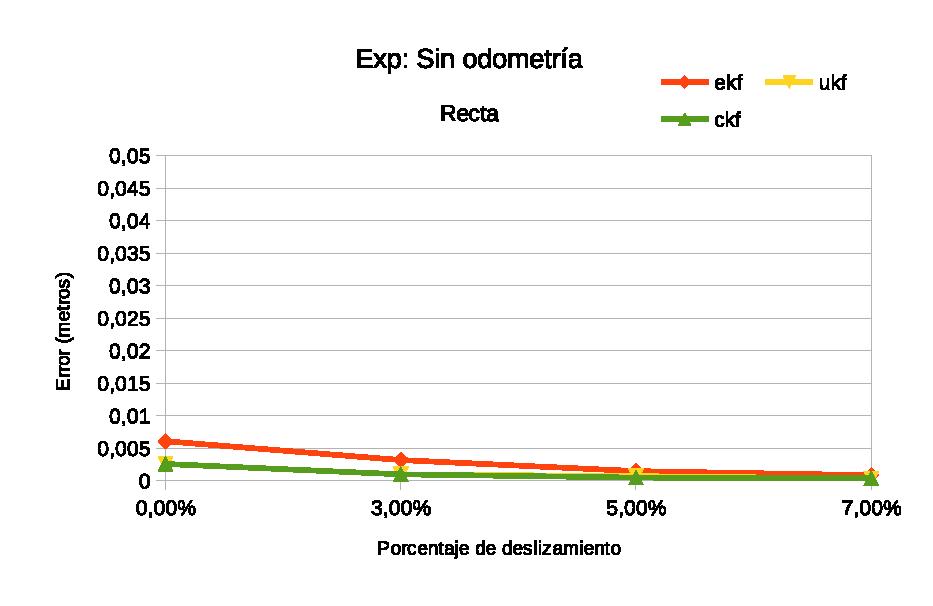
\includegraphics[scale=0.6]{Grafico1_1}
\caption{Experimento recta sin odometría} \label{Grafico1_1}
\end{figure}
\begin{figure}[ht!]
\centering
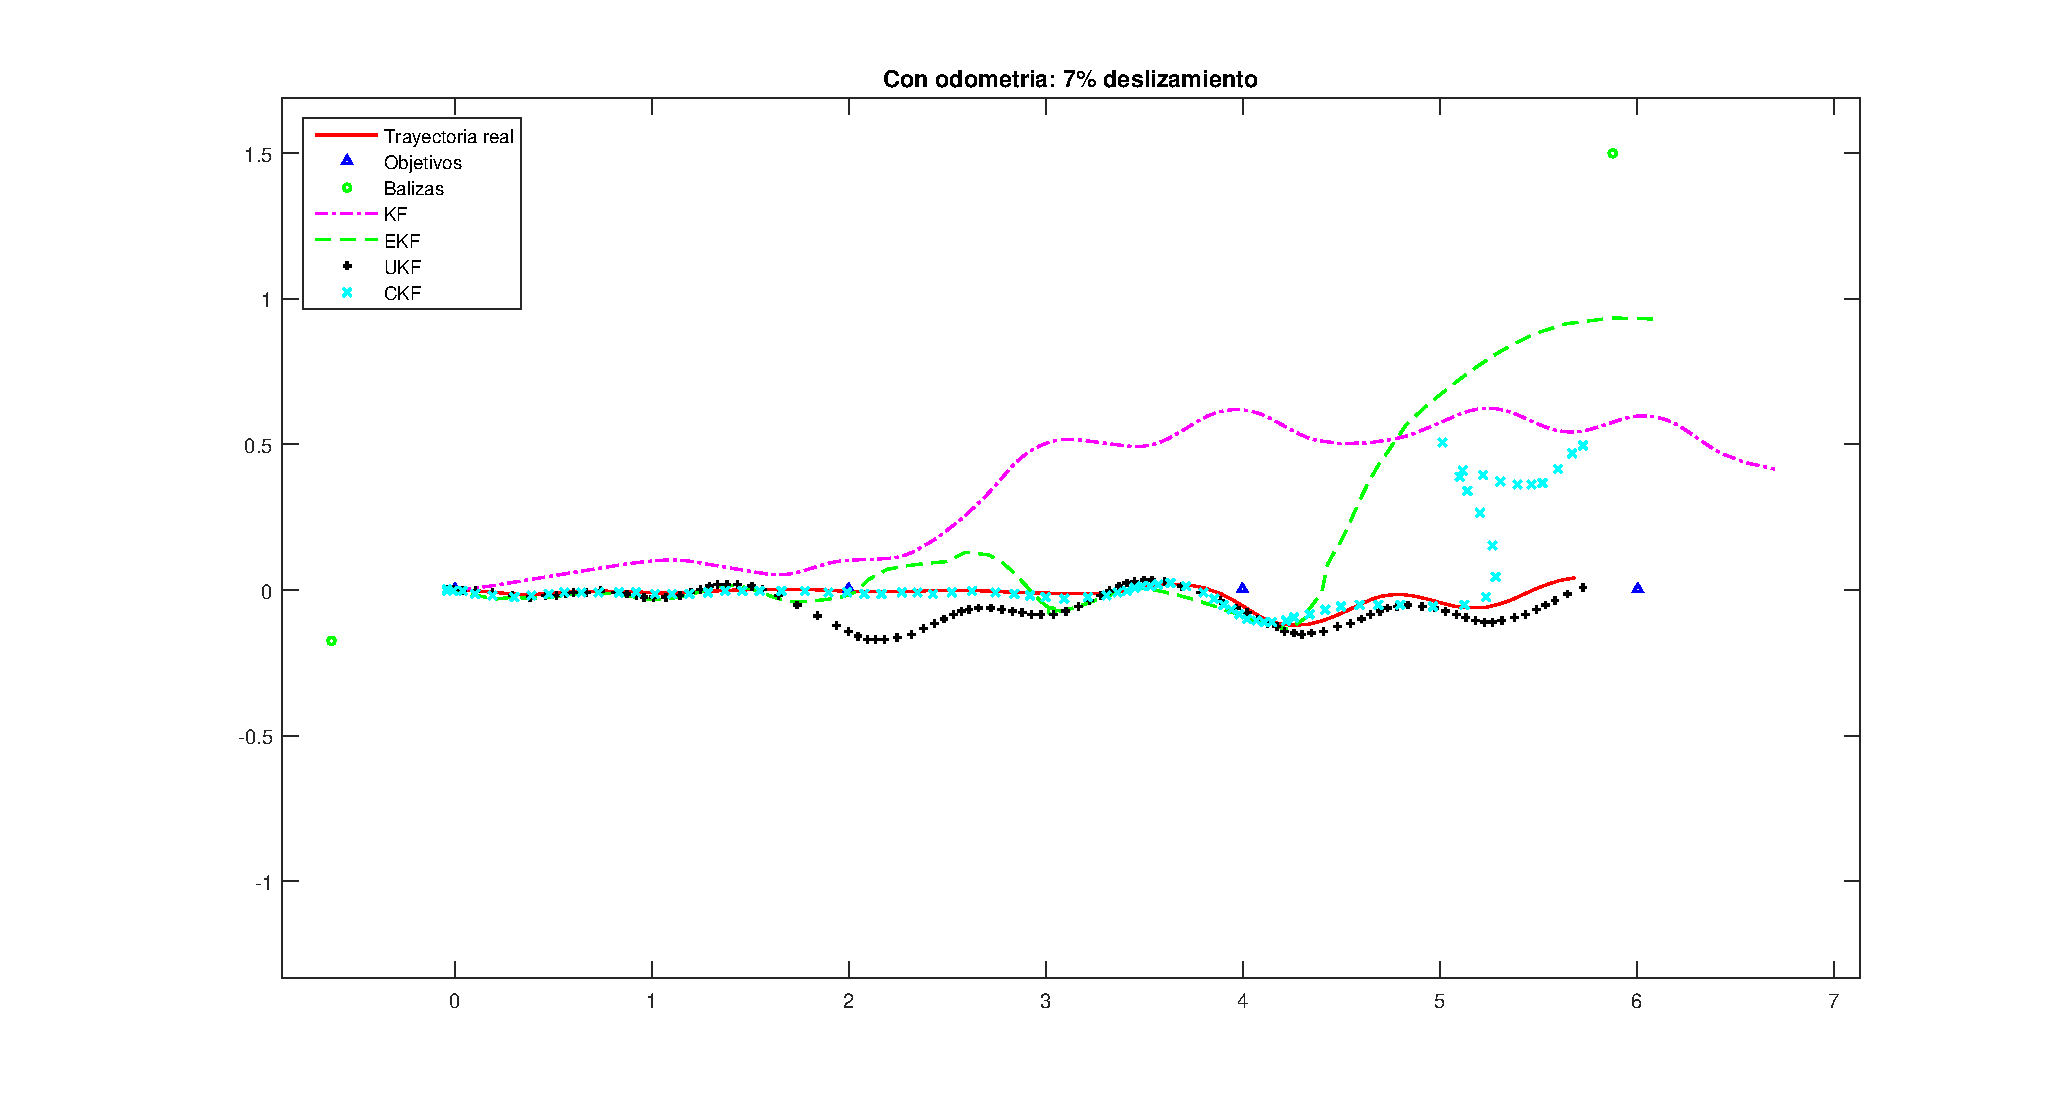
\includegraphics[scale=0.4]{Figura_Recta_Odometria}
\caption{Trayectoria recta con odometría} \label{Figura1}
\end{figure}

\begin{figure}[ht!]
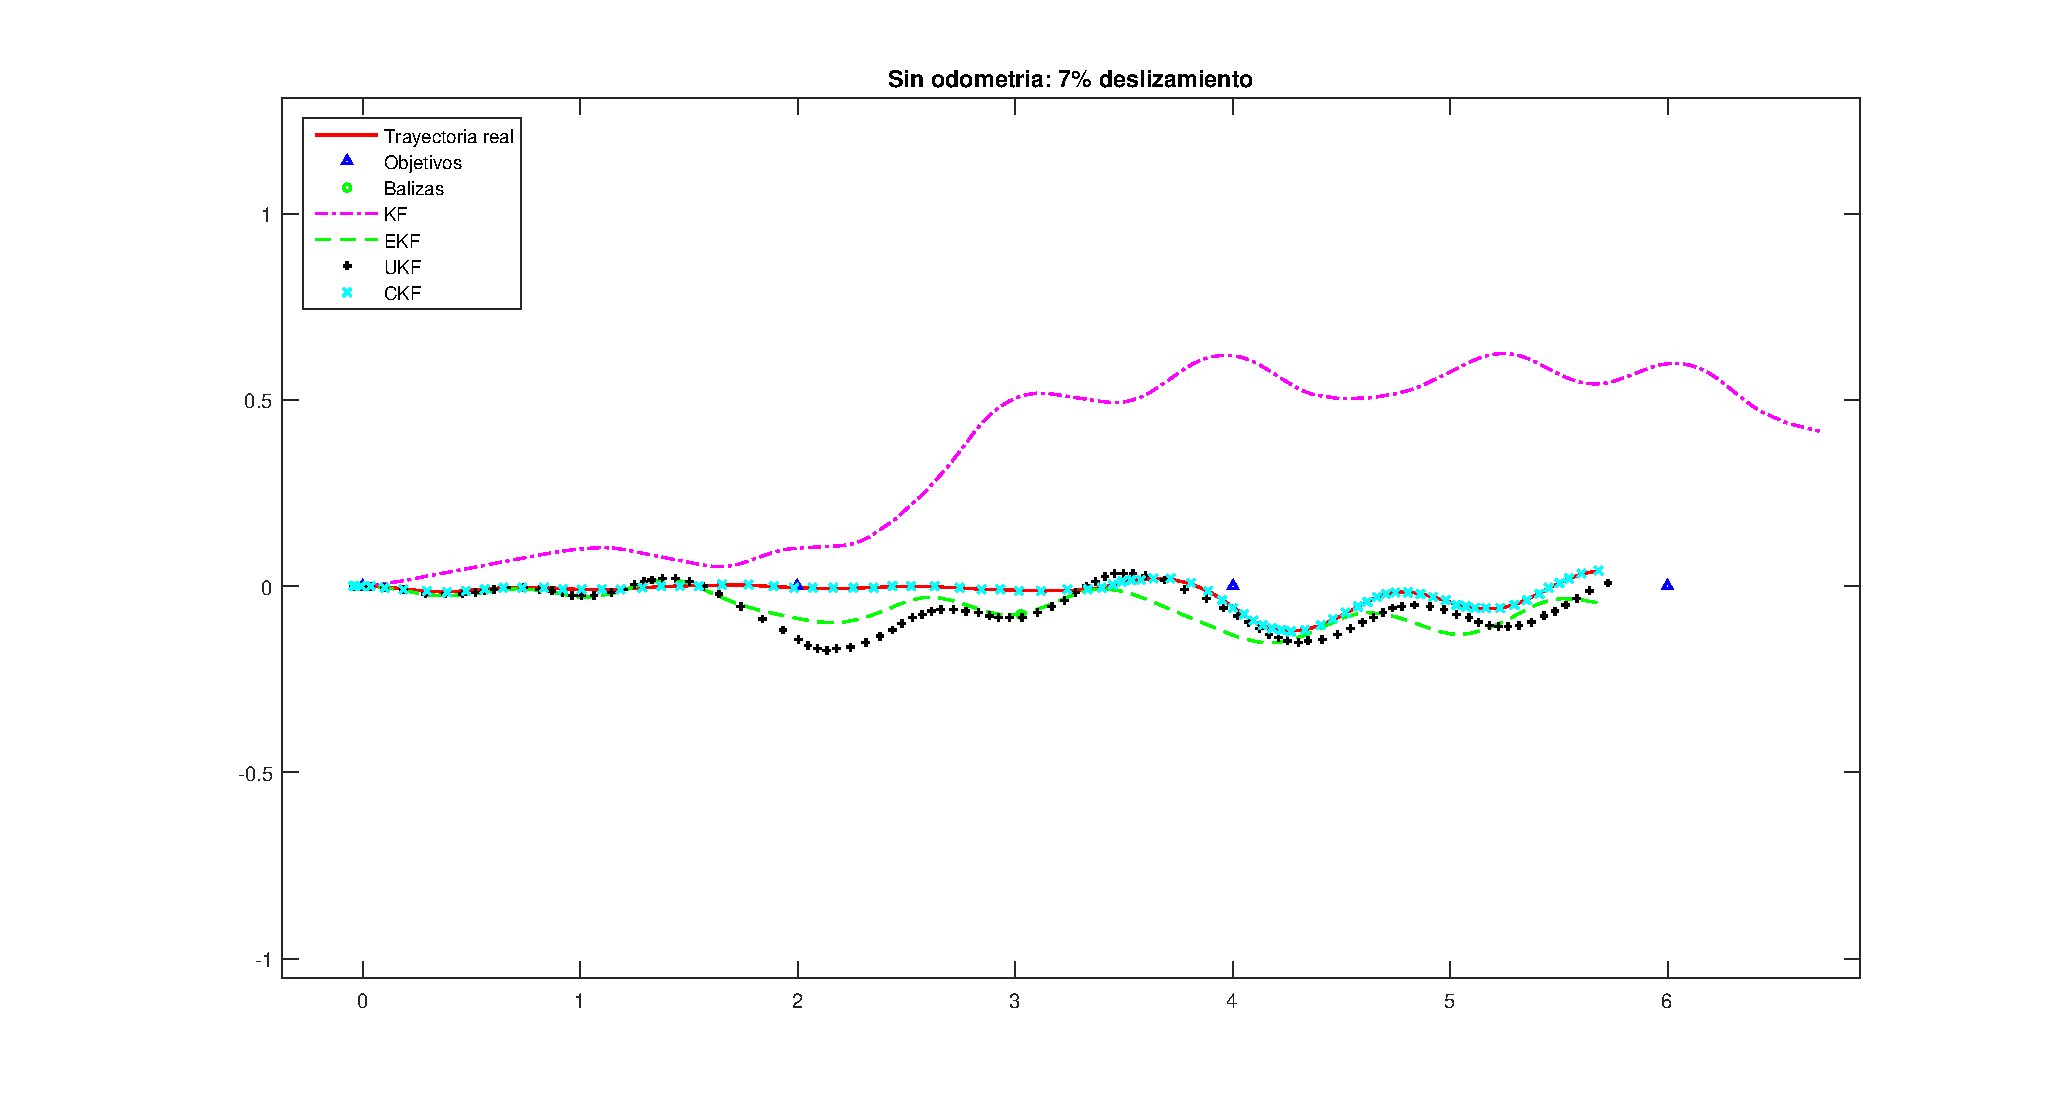
\includegraphics[scale=0.4]{Figura_Recta_SinOdometria}
\caption{Trayectoria recta sin odometría} \label{Figura1_1}
\end{figure}

En las figuras \ref{Grafico1}, \ref{Figura1}, \ref{Grafico1_1} y \ref{Figura1_1}, podemos ver los resultados obtenidos para las dos tandas de experimentos, es decir, con y sin odometría.
Vemos que en ambos casos el \ac{UKF} es el que presenta el menor error, seguido del \ac{CKF} y posteriormente por el \ac{EKF}.
Con respecto al filtro clásico de Kalman vemos que su estimación no es del todo correcta, aunque el error para el 7\% de deslizamiento es de 0.93 metros, y si pensamos que solamente hemos tenido en cuenta la odometría para la estimación este valor no es tan malo.
Otra observación interesante entre las figuras \ref{Grafico1} y \ref{Grafico1_1} es que cuando no implementamos la odometría la estimación es mejor.
Esto es debido a que los deslizamientos hacen que la odometría no sea una información válida y por lo tanto en ese caso sería mejor no implementarla como demuestra la figura \ref{Grafico1_1} donde el máximo error obtenido es de 0.006 metros, lo que significa que hemos tenido una estimación casi perfecta.
% * <amorellg@ull.edu.es> 2016-06-06T19:55:49.119Z:
%
% > Esto es debido a que los deslizamientos hacen que la odometría no sea una información válida y por lo tanto en ese caso sería mejor no implementarla como demuestra la figura \ref{Grafico1_1} donde el máximo error obtenido es de 0.006 metros, lo que significa que hemos tenido una estimación casi perfecta.
%
% Agrupa mejor las gráficas y figuras por su naturaleza, para que sea más fácil comparar el error con y sin odometría y la gráfica de la trayectoria con y sin odometría
%
% ^ <alu0100765755@ull.edu.es> 2016-06-07T09:29:54.802Z:
%
% Hecho !!
%
% ^ <alu0100765755@ull.edu.es> 2016-06-07T09:29:56.442Z.
Es muy importante tener en cuenta que las trayectorias reales mostradas en las figuras \ref{Figura1} y \ref{Figura1_1} no son las trayectorias que han seguido todos los filtros ya que al trabajar con deslizamientos para cada filtro la trayectoria se ha podido ver afectada de distinta manera (por ejemplo si el robot ha deslizado en otra dirección), por esta razón hemos realizado baterías de experimentos y luego hemos obtenido la media del error, con lo cual la trayectoria mostrada es meramente orientativa para saber la forma de la ruta tomada por nuestro robot y no como referencia comparativa.
% * <amorellg@ull.edu.es> 2016-06-06T19:57:13.535Z:
%
% >  figuras \ref{Figura1} y
%
% en la figura 2.8 del error sin odometría, la escala del error es demasiado pequeña y parece que haya más diferencia, cuando estamos hablando del 3er decimal, en la frontera del error numérico del motor de física...  Mira a ver cómo queda poniéndolo 
%
% ^ <alu0100765755@ull.edu.es> 2016-06-07T09:35:01.212Z:
%
% Cambiamos el tamaño de los ejes y listo !
%
% ^ <alu0100765755@ull.edu.es> 2016-06-07T09:43:10.111Z.
\subsection{Resultados para la trayectoria cuadrada}
Para las trayectorias cuadradas la configuración ha sido la misma que para las rectas, los resultados se muestran en las figuras \ref{Grafico2}, \ref{Figura2}, \ref{Grafico2_2} y \ref{Figura2_2}.
\begin{figure}[ht!]
\centering
\includegraphics[scale=0.6]{Grafico2}
\caption{Experimento cuadrado con odometría} \label{Grafico2}
\end{figure}
\begin{figure}[ht!]
\centering
\includegraphics[scale=0.6]{Grafico2_2}
\caption{Experimento cuadrado sin odometría} \label{Grafico2_2}
\end{figure}
\begin{figure}[ht!]
\centering
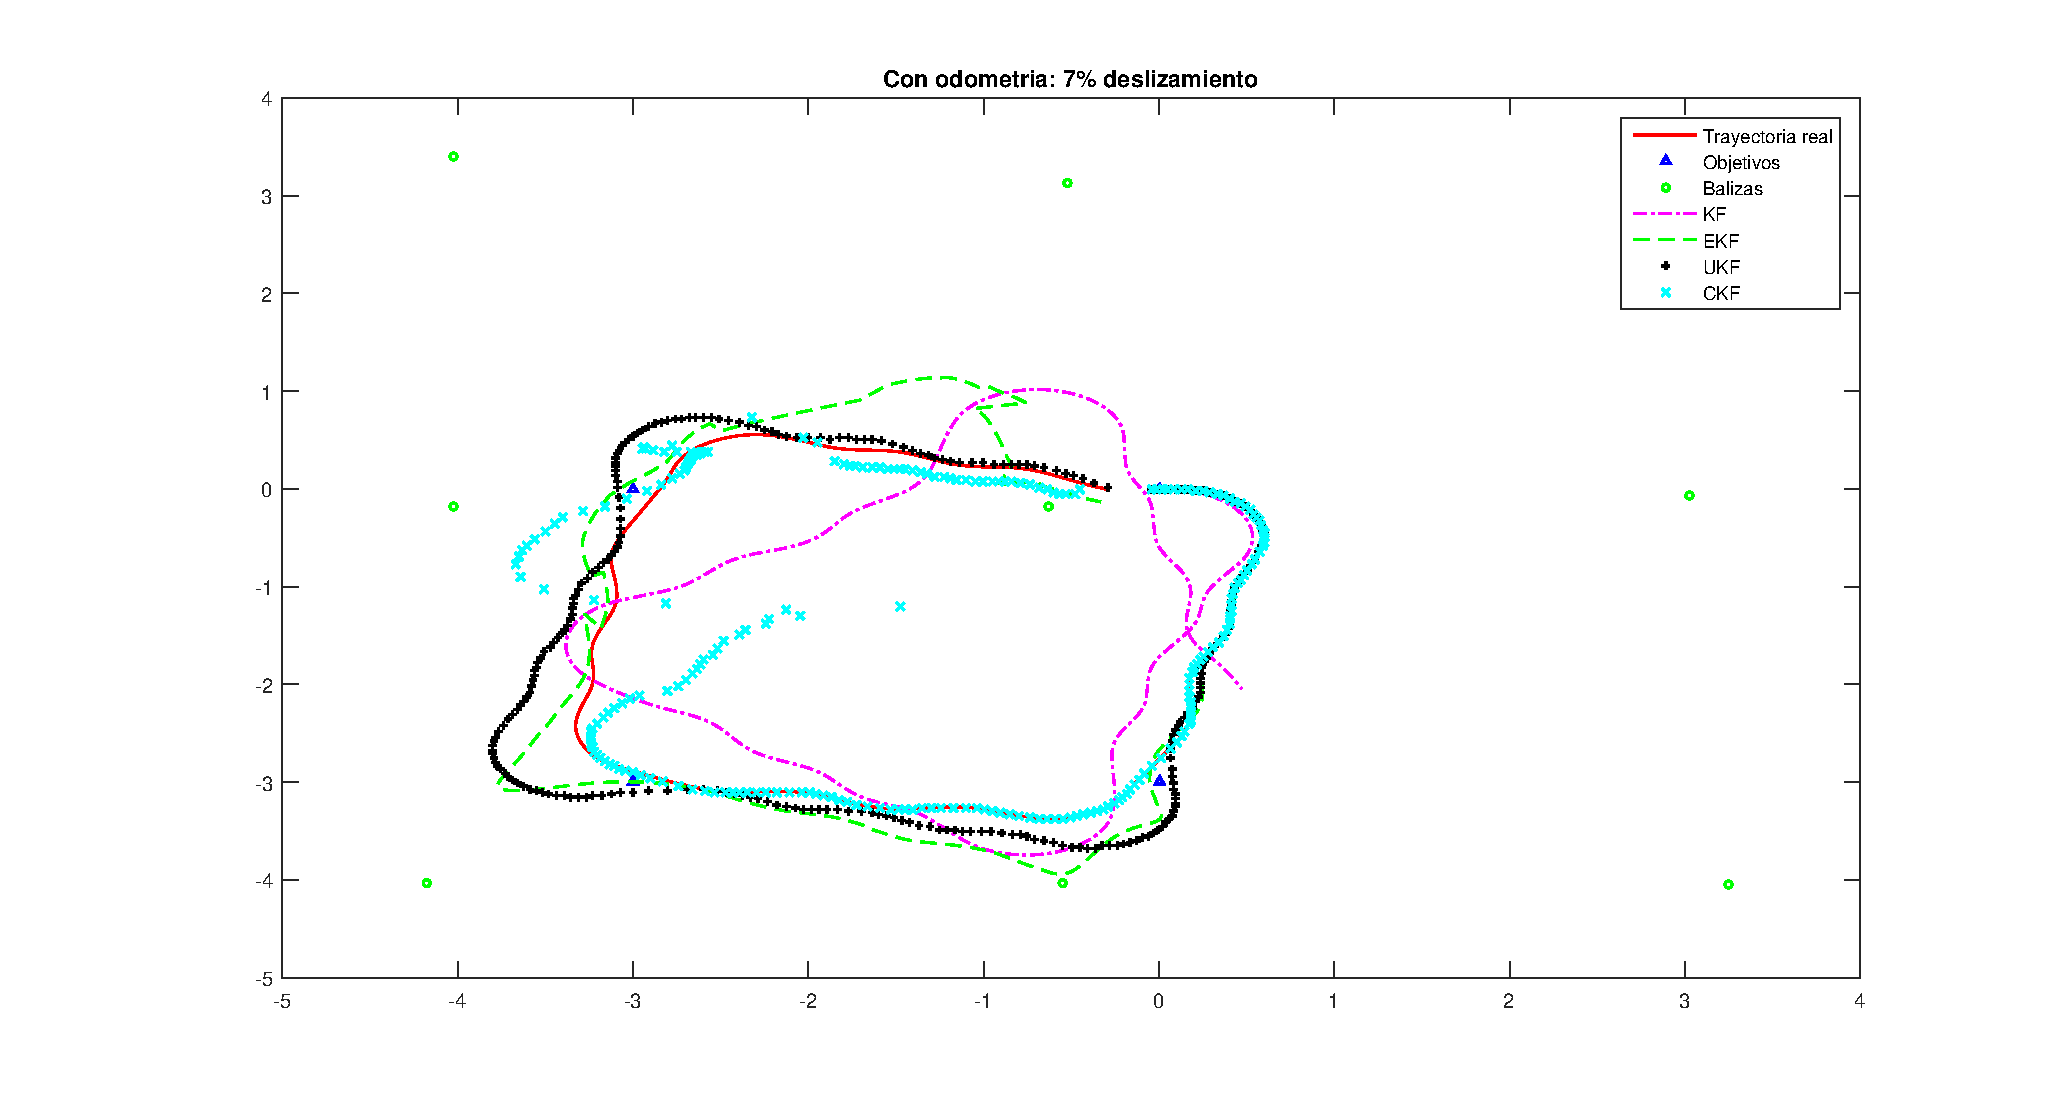
\includegraphics[scale=0.4]{Figura_Cuadrado_Odometria}
\caption{Trayectoria cuadrada con odometría} \label{Figura2}
\end{figure}
\begin{figure}[ht!]
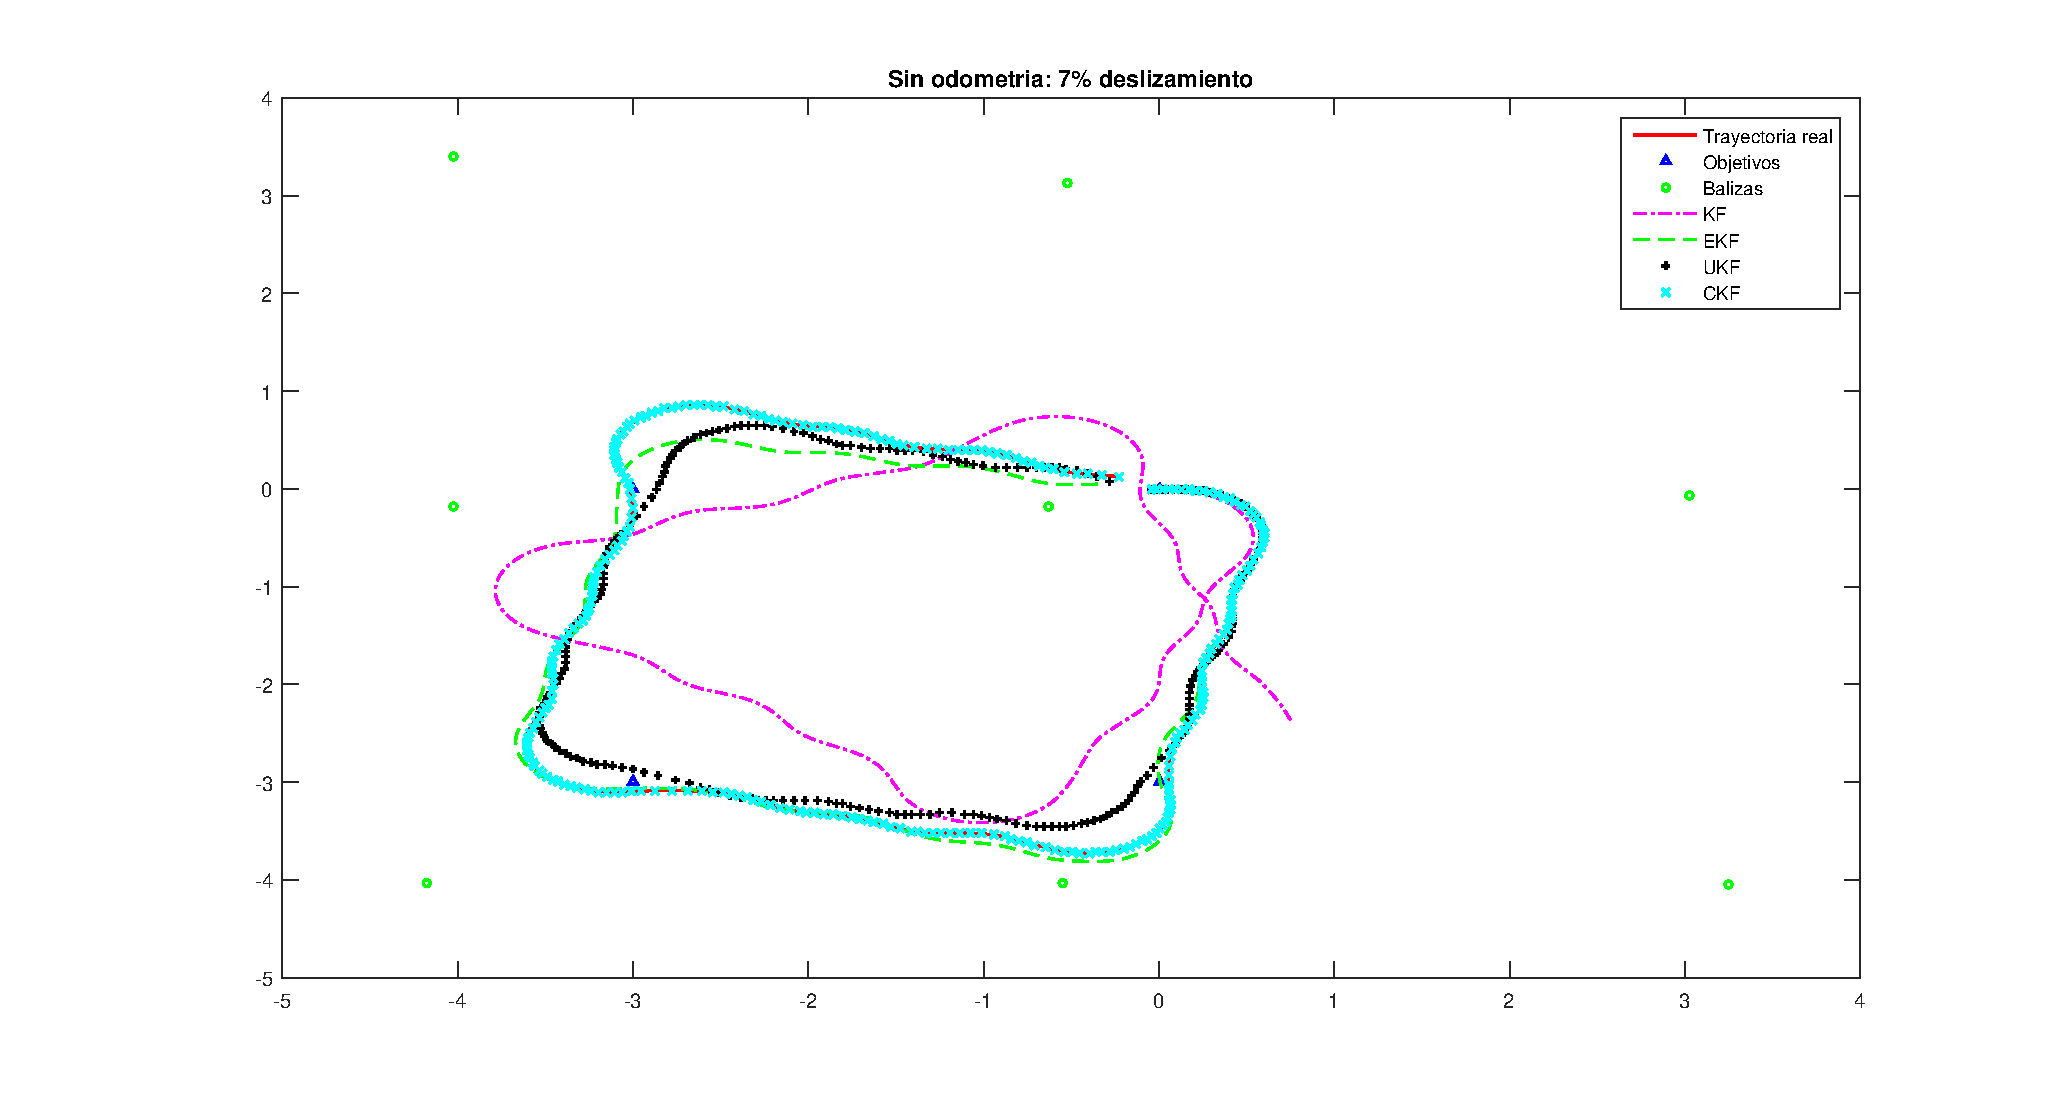
\includegraphics[scale=0.4]{Figura_Cuadrado_SinOdometria}
\caption{Trayectoria cuadrada sin odometría} \label{Figura2_2}
\end{figure}
En este experimento llegamos a unas conclusiones muy parecidas a las del experimento de las rectas.
Vemos que los resultados en la implementación de la odometría \ref{Grafico2} resulta más errónea a medida que el deslizamiento aumenta.
En cambio cuando no implementamos la odometría los errores obtenidos son muy ínfimos como vemos en la figura \ref{Grafico2_2}.
En este experimento el filtro que ha presentado el error más bajo ha sido el \ac{EKF} en el experimento sin la implementación de la odometría como vemos en la figura \ref{Grafico2_2}.
\subsection{Resultados para la trayectoria senoidal}
Los resultados de este experimento son mostrados en las figuras \ref{Grafico3}, \ref{Figura3}, \ref{Grafico3_3} y \ref{Figura3_3}.
\begin{figure}[ht!]
\centering
\includegraphics[scale=0.6]{Grafico3}
\caption{Experimento seno con odometría} \label{Grafico3}
\end{figure}
\begin{figure}[ht!]
\centering
\includegraphics[scale=0.6]{Grafico3_3}
\caption{Experimento seno sin odometría} \label{Grafico3_3}
\end{figure}
\begin{figure}[ht!]
\centering
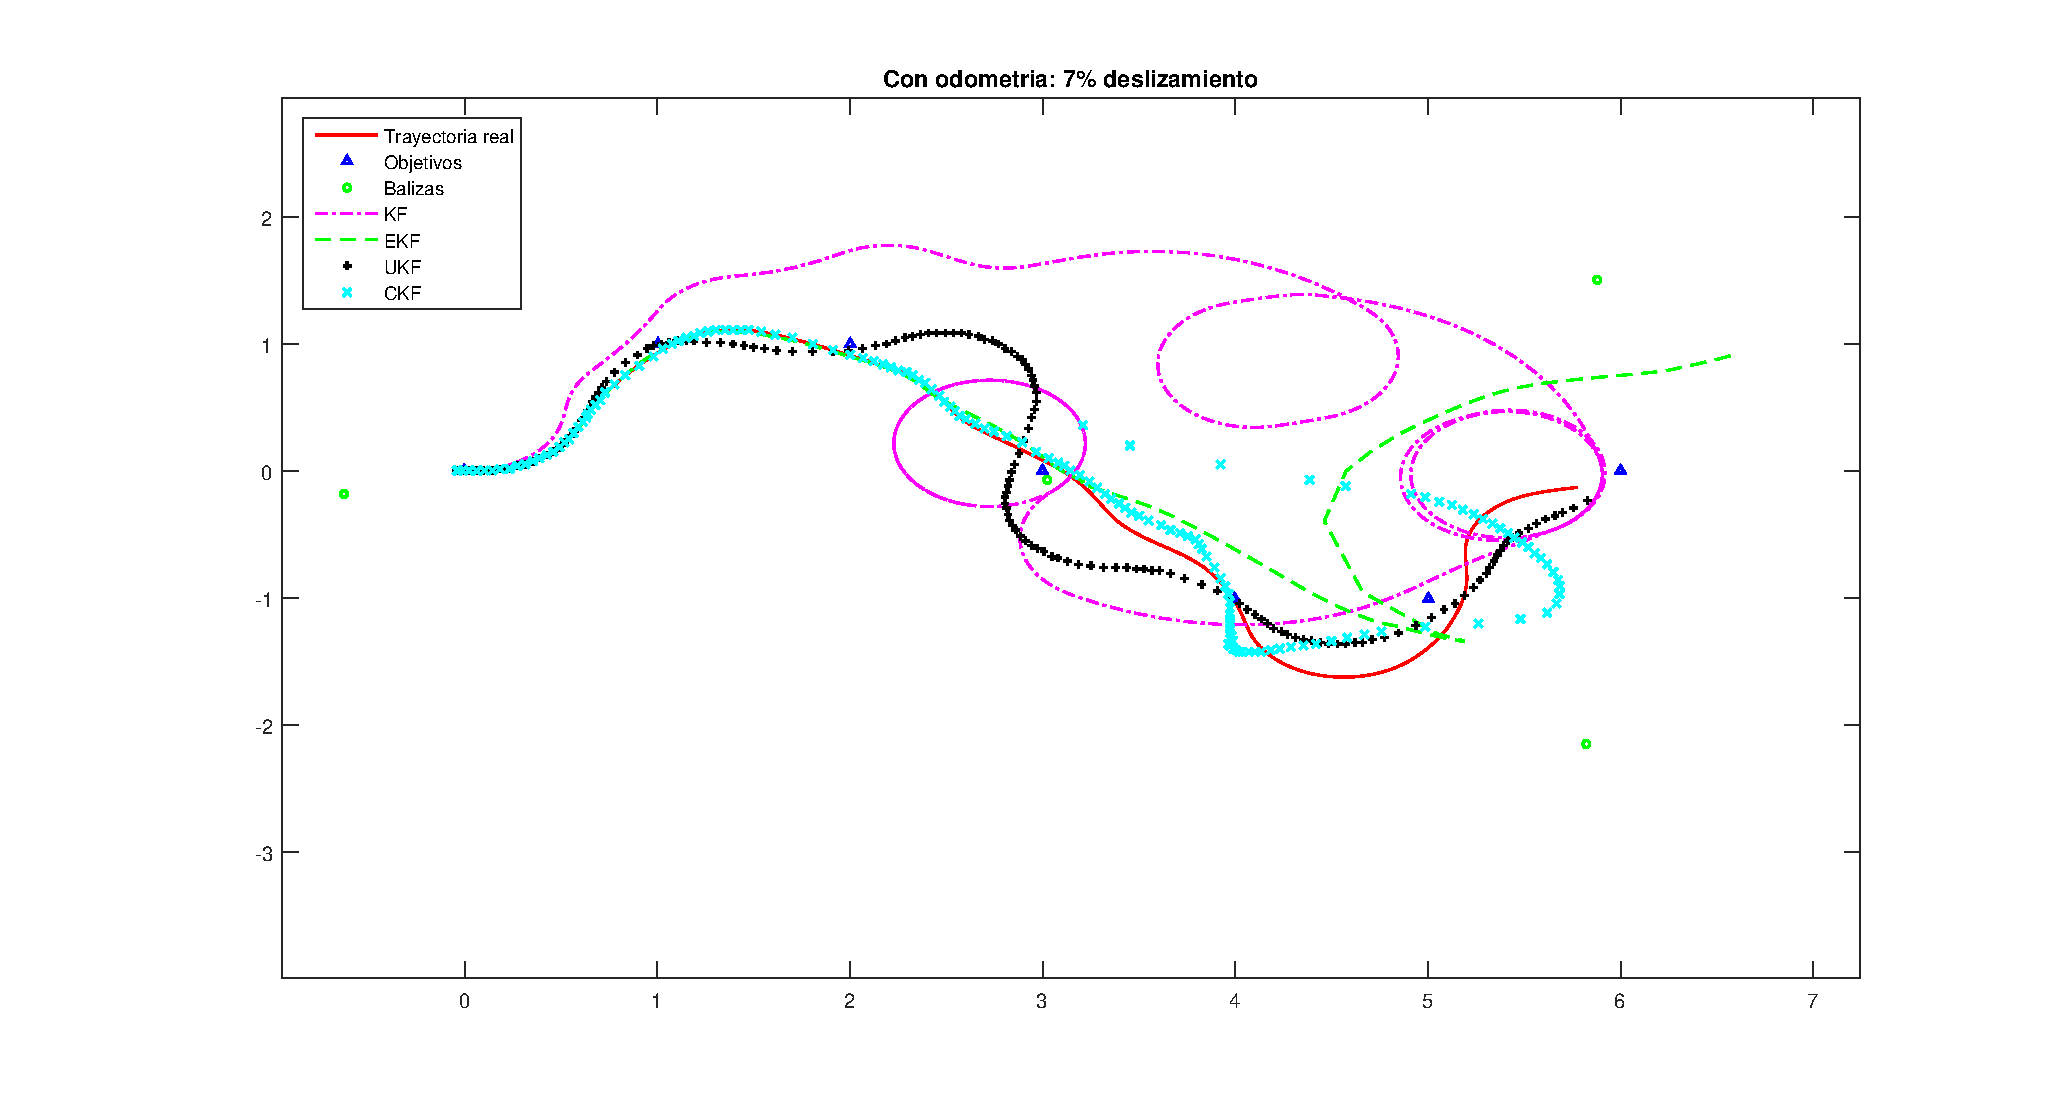
\includegraphics[scale=0.4]{Figura_Seno_Odometria}
\caption{Trayectoria senoidal con odometría} \label{Figura3}
\end{figure}

\begin{figure}[ht!]
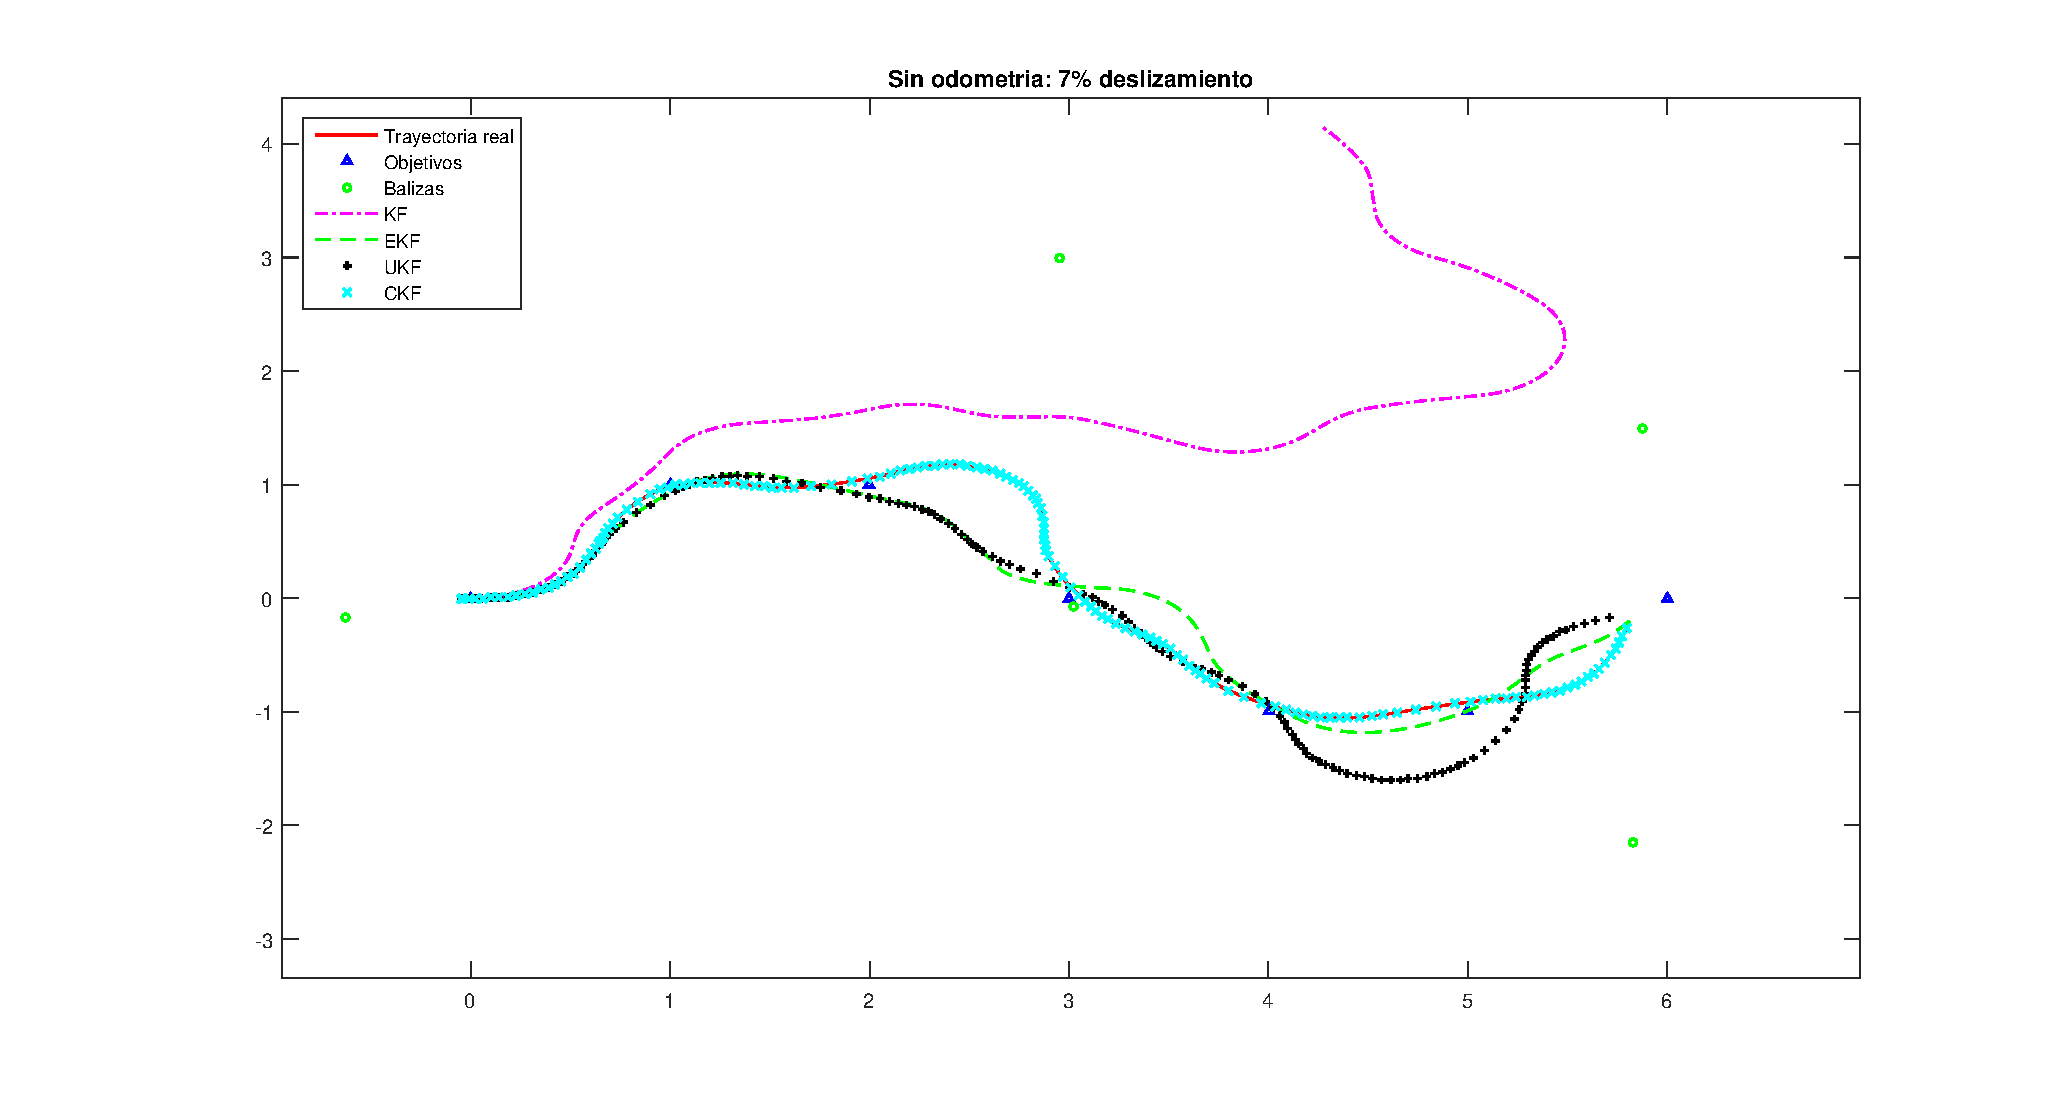
\includegraphics[scale=0.4]{Figura_Seno_SinOdometria}
\caption{Trayectoria senoidal sin odometría} \label{Figura3_3}
\end{figure}
Para esta serie de pruebas llegamos a las mismas conclusiones que para todas las anteriores, por lo que podemos concluir que la odometría puede ser una información peligrosa si trabajamos con deslizamientos muy grandes.
Por otra parte hay que notar que en las figuras \ref{Figura3} y \ref{Figura3_3} el filtro claśico de Kalman tiene un comportamiento muy diferente e igualmente erróneo, esto es debido a que en cada simulación el motor de físicas del simulador hace que el robot pueda deslizar más o menos en distintas zonas además de que nuestro planificador de rutas puede llegar a tomar diferentes decisiones en función de los deslizamientos, por esta razón el aspecto de la simulación es diferente y no debemos tomar las trayectorias mostradas en las figuras \ref{Figura3} y \ref{Figura3_3} como representación de la serie de experimentos, estas figuras son meramente orientativas y escogidas al azar dentro de la serie de pruebas realizadas.

La conclusión para esta serie de experimentos es la siguiente: \textbf{La odometría es una información que puede ayudar a localizarnos con éxito, pero con la existencia de deslizamientos puede ocurrir que esta información contribuya a la deslocalización.}

\section{Experimento 2: Ruido en las medidas}
En esta sección de experimentos veremos como afecta el ruido en los sensores a la estimación que realizan los filtros.
Representaremos los resultados por medio de gráficos para una mejor comprensión y análisis de estos.
Además representaremos las trayectorias seguidas por los filtros para el peor caso de estimación y usaremos dos funciones de medida distintas de las que ya hemos hablado: la función de medida de distancia (ecuación \ref{Modelo_distancia}) y la de medida de ángulos (ecuación \ref{Modelo_angulo}).
La sintonización de los filtros y sus parámetros es la misma que para el experimento 1.
Además el deslizamiento se fijará en un $0\%$ para esta serie de pruebas.
% * <amorellg@ull.edu.es> 2016-06-06T20:30:33.632Z:
%
% > .
%
% añade, para recordar: "en estos experimentos fijamos el valor de deslizamiento en XX%"
%
% ^ <alu0100765755@ull.edu.es> 2016-06-07T09:44:54.991Z.
\subsection{Resultados para la trayectoria recta}
En las figuras \ref{Grafico4}, \ref{Figura4}, \ref{Grafico4_4} y \ref{Figura4_4} podemos ver los resultados obtenidos.
\begin{figure}[ht!]
\centering
\includegraphics[scale=0.6]{Grafico4}
\caption{Experimento recta función de medida de distancia} \label{Grafico4}
\end{figure}
\begin{figure}[ht!]
\centering
\includegraphics[scale=0.6]{Grafico4_4}
\caption{Experimento recta función de medida de ángulos} \label{Grafico4_4}
\end{figure}
\begin{figure}[ht!]
\centering
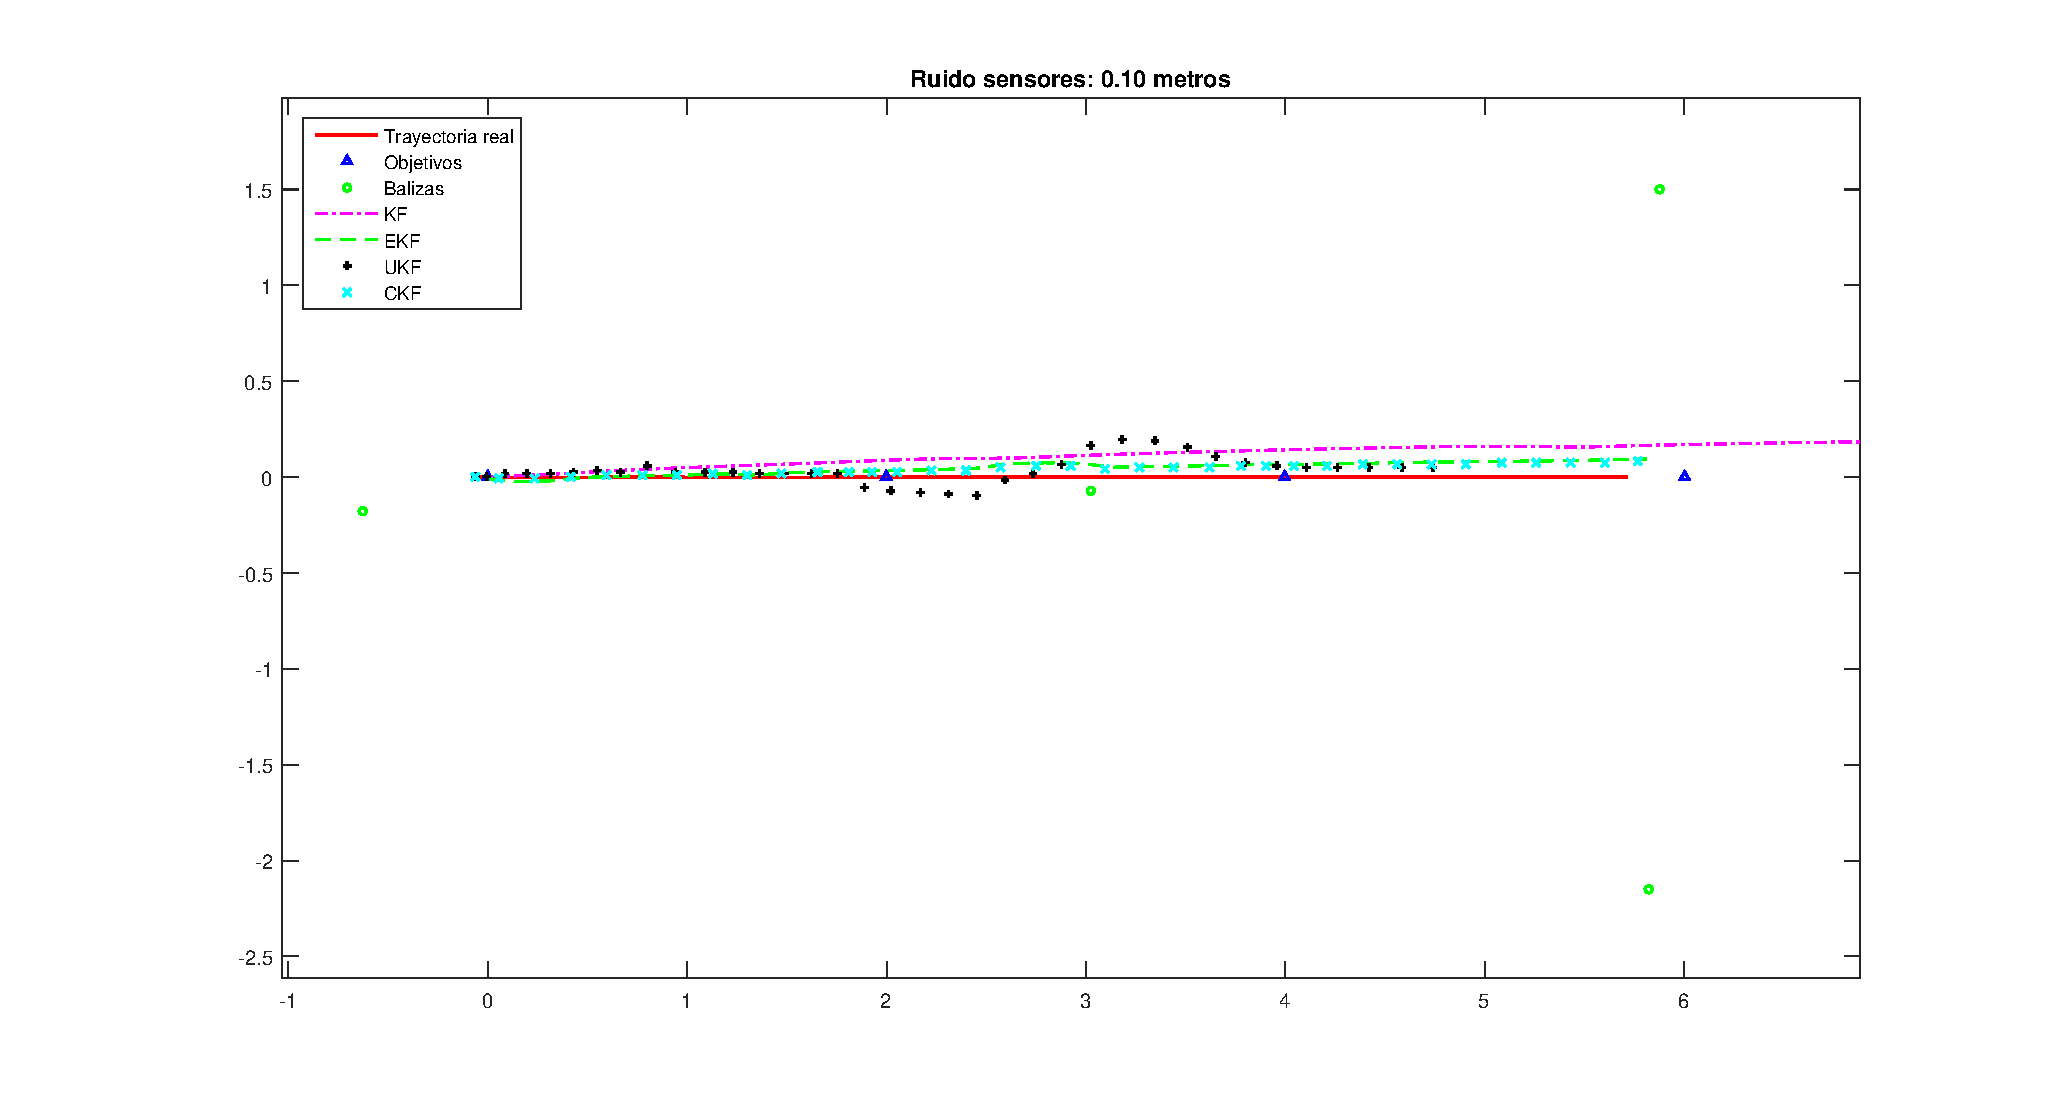
\includegraphics[scale=0.4]{Figura4}
\caption{Trayectoria recta función de medida de distancia} \label{Figura4}
\end{figure}

\begin{figure}[ht!]
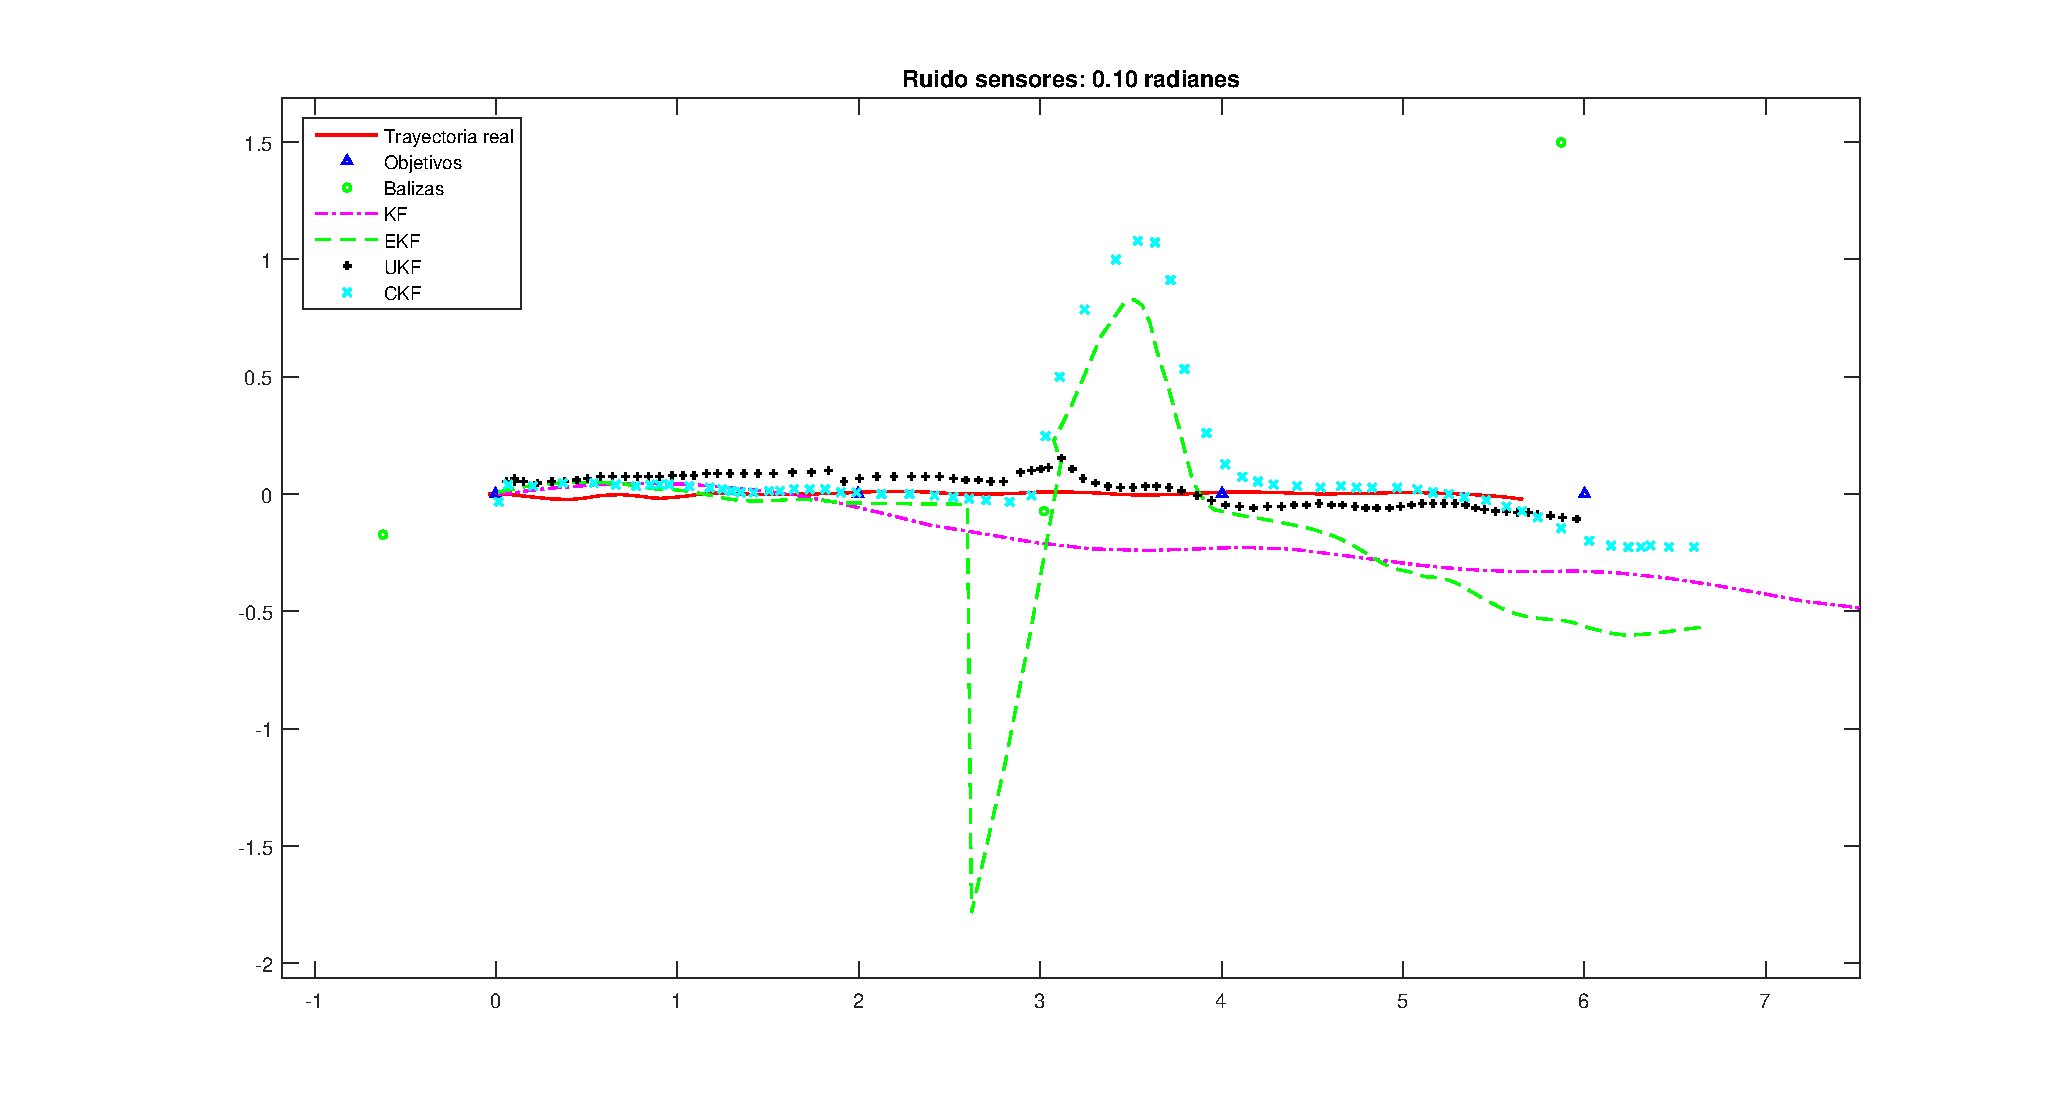
\includegraphics[scale=0.4]{Figura4_4}
\caption{Trayectoria recta función de medida de ángulos} \label{Figura4_4}
\end{figure}
Podemos ver claramente en la figura \ref{Figura4_4} que para el modelo de medida de ángulos existen muchas singularidades que hacen que la estimación sea totalmente errónea, como es el caso del \ac{EKF} o el \ac{UKF} en dicha figura.
Además si comparamos las figuras \ref{Grafico4} y \ref{Grafico4_4} vemos que los errores son más grandes para la función de medida de ángulos que para la función de medida de distancias y algunos casos es debido a las singularidades.
El \ac{CKF} ha sido el filtro que menor error ha tenido en la figura \ref{Grafico4} mientras que para el modelo de medida de ángulos (figura \ref{Grafico4_4}) ha sido el \ac{UKF}.
Por último, como era de esperar el error en la localización tiende a aumentar a medida que aumenta el ruido presente en los sensores, lo cuál es lógico.
También vemos que para el \ac{UKF} es menor el error si la función de medida utilizada es la de ángulos, para el \ac{CKF} y el \ac{EKF} pasa totalmente lo contrario.

\subsection{Resultados para la trayectoria cuadrada}
Las figuras \ref{Grafico5}, \ref{Figura5}, \ref{Grafico5_5} y \ref{Figura5_5} muestran los resultados para esta serie de experimentos.
La configuración utilizada ha sido la misma que para todas las pruebas hasta el momento.
\begin{figure}[ht!]
\centering
\includegraphics[scale=0.6]{Grafico5}
\caption{Experimento cuadrado función de medida de distancia} \label{Grafico5}
\end{figure}
\begin{figure}[ht!]
\centering
\includegraphics[scale=0.6]{Grafico5_5}
\caption{Experimento cuadrado función de medida de ángulos} \label{Grafico5_5}
\end{figure}
\begin{figure}[ht!]
\centering
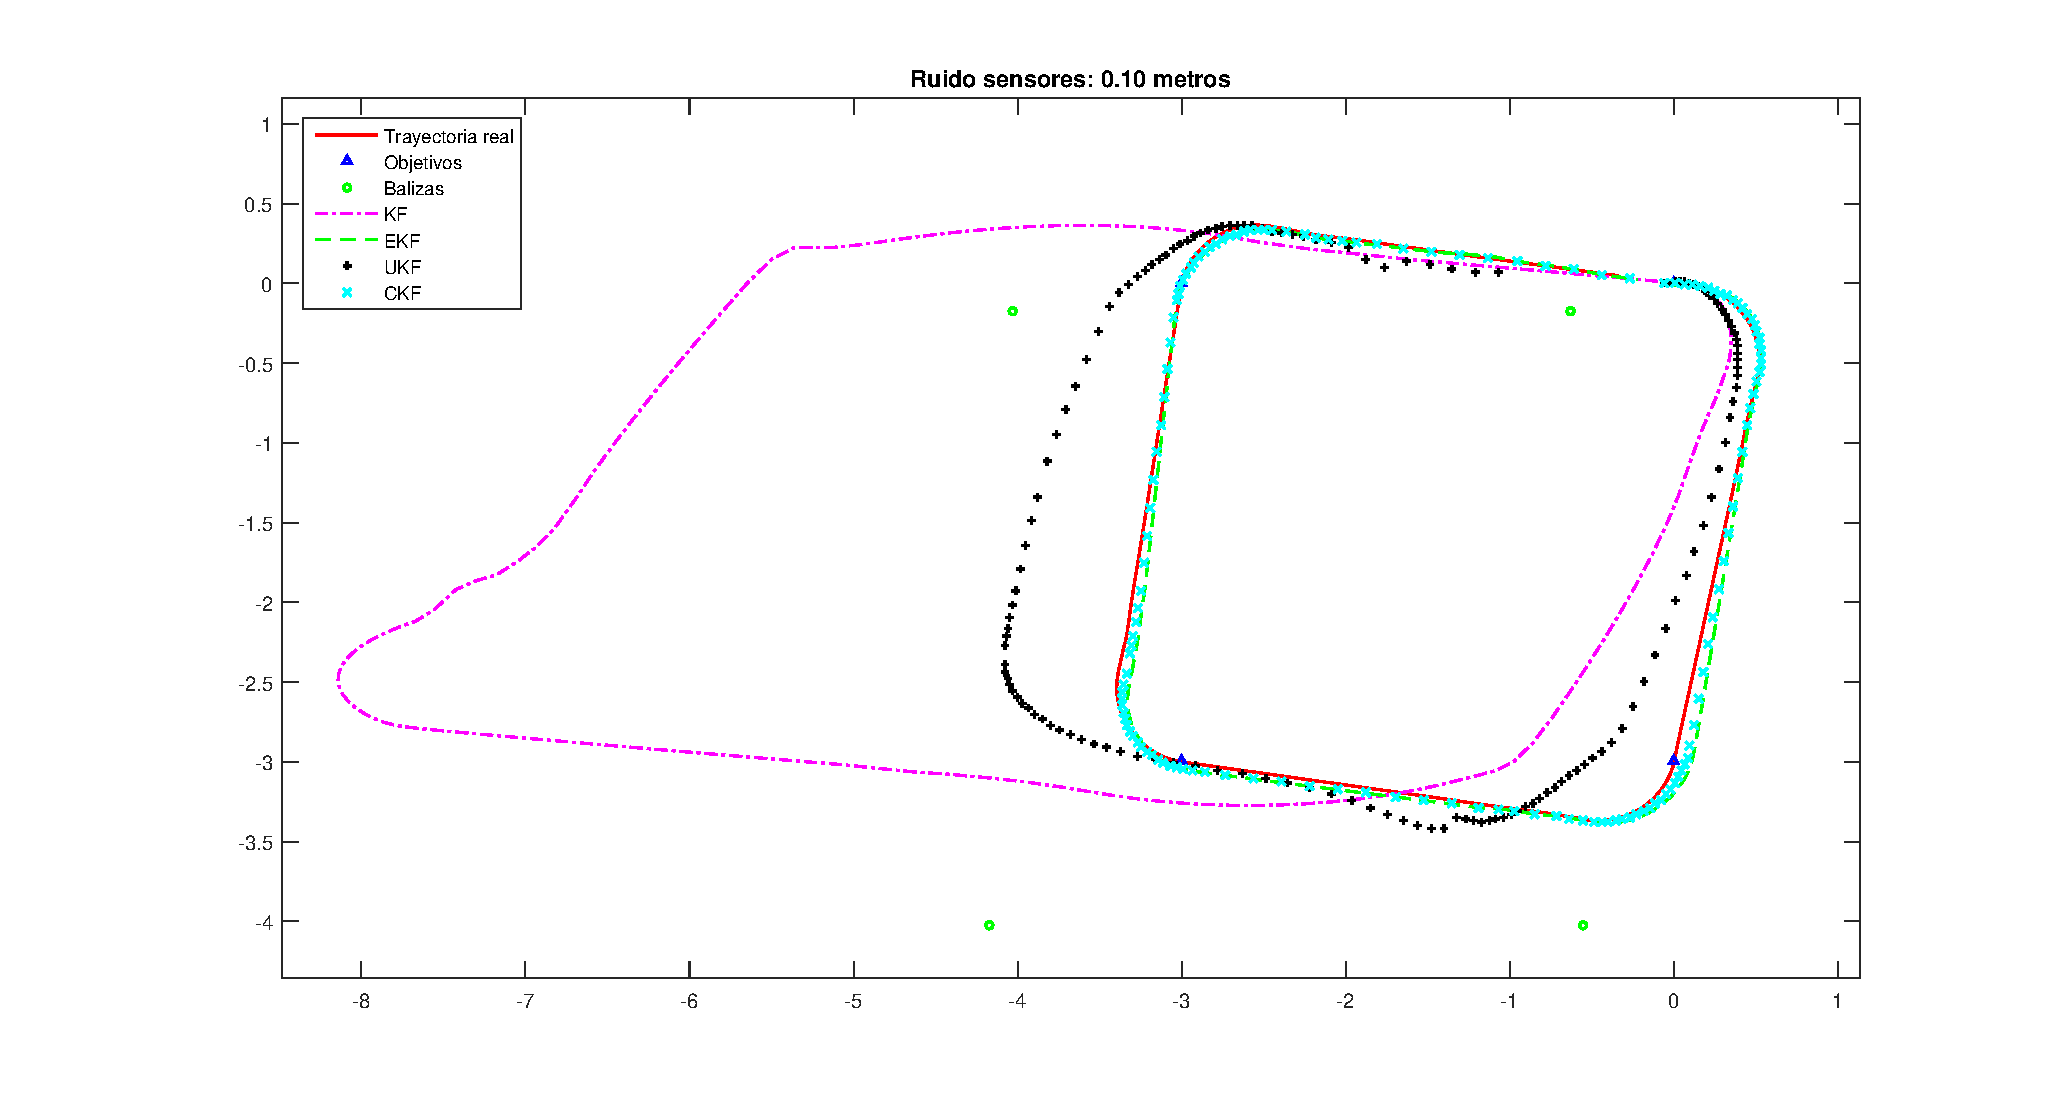
\includegraphics[scale=0.4]{Figura5}
\caption{Trayectoria cuadrada función de medida de distancia} \label{Figura5}
\end{figure}

\begin{figure}[ht!]
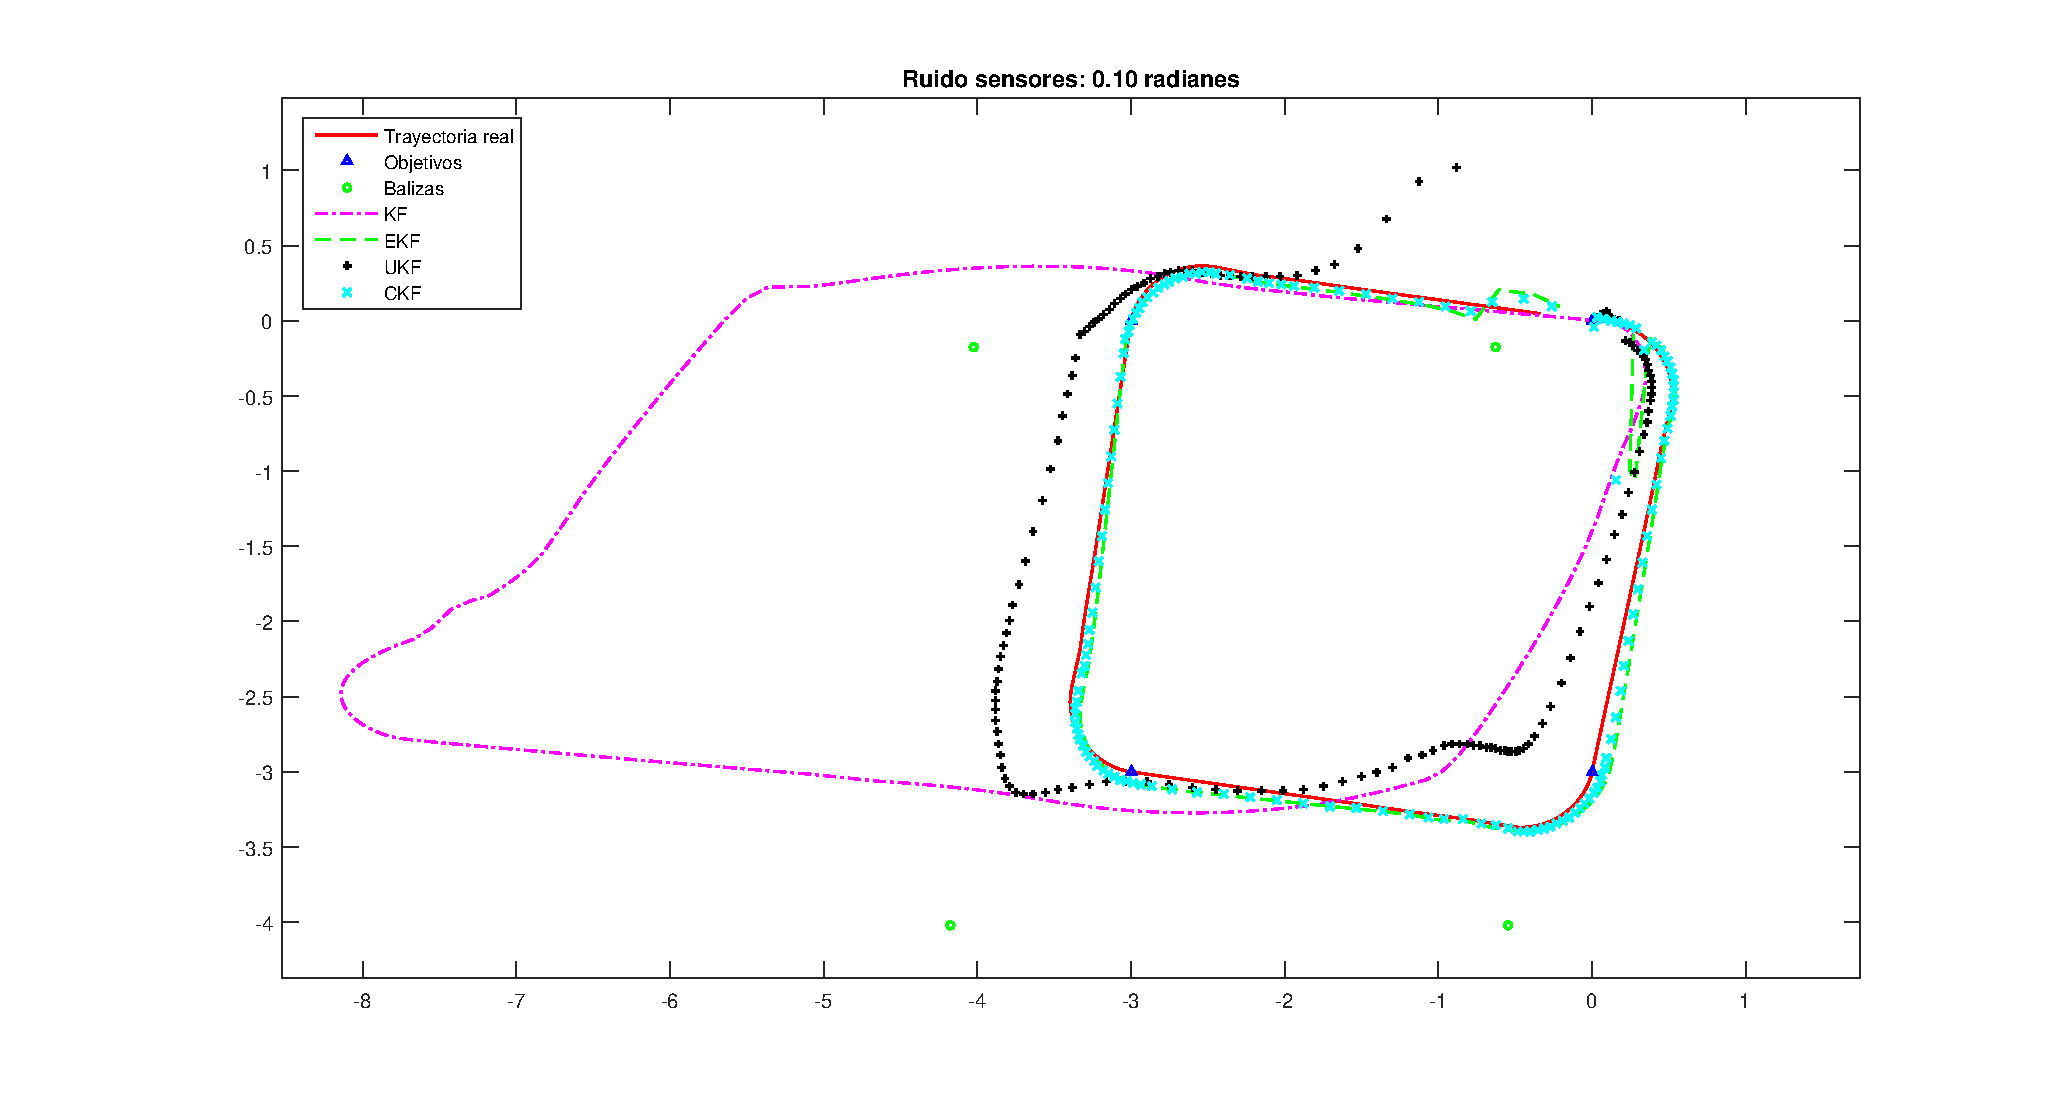
\includegraphics[scale=0.4]{Figura5_5}
\caption{Trayectoria cuadrada función de medida de ángulos} \label{Figura5_5}
\end{figure}
En este caso los resultados se repiten con respecto al primer experimento de esta serie.
Podemos ver que el \ac{UKF} presenta errores mayores cuando usa la función de medida de distancia, además también podemos observar ciertas singularidades en la figura \ref{Figura5_5} provocadas por la función de medida de ángulos.
En \ac{CKF} ha sido el filtro que menor error ha presentado en general.
En la figura \ref{Figura5} vemos como el error aumenta a medida que lo hace el ruido en los sensores, en cambio en la figura \ref{Figura5_5} vemos todo lo contrario y esto es debido a que probablemente para el primer experimento de la serie las singularidades hayan hecho aumentar el error obtenido.
Aun con lo anterior para este caso la función de medida de distancias tiene un mejor comportamiento ya que los errores obtenidos de forma global son menores como vemos en la figura \ref{Grafico5} en comparación con \ref{Grafico5_5}, por lo que se demuestra que la función de medida de distancias es más eficiente que la de medida de ángulos.
\subsection{Resultados para la trayectoria senoidal}
Los resultados de esta serie de experimentos pueden verse en las figuras \ref{Grafico6}, \ref{Figura6}, \ref{Grafico6_6} y \ref{Figura6_6}.
\begin{figure}[ht!]
\centering
\includegraphics[scale=0.6]{Grafico6}
\caption{Experimento seno función de medida de distancia} \label{Grafico6}
\end{figure}
\begin{figure}[ht!]
\centering
\includegraphics[scale=0.6]{Grafico6_6}
\caption{Experimento seno función de medida de ángulos} \label{Grafico6_6}
\end{figure}
\begin{figure}[ht!]
\centering
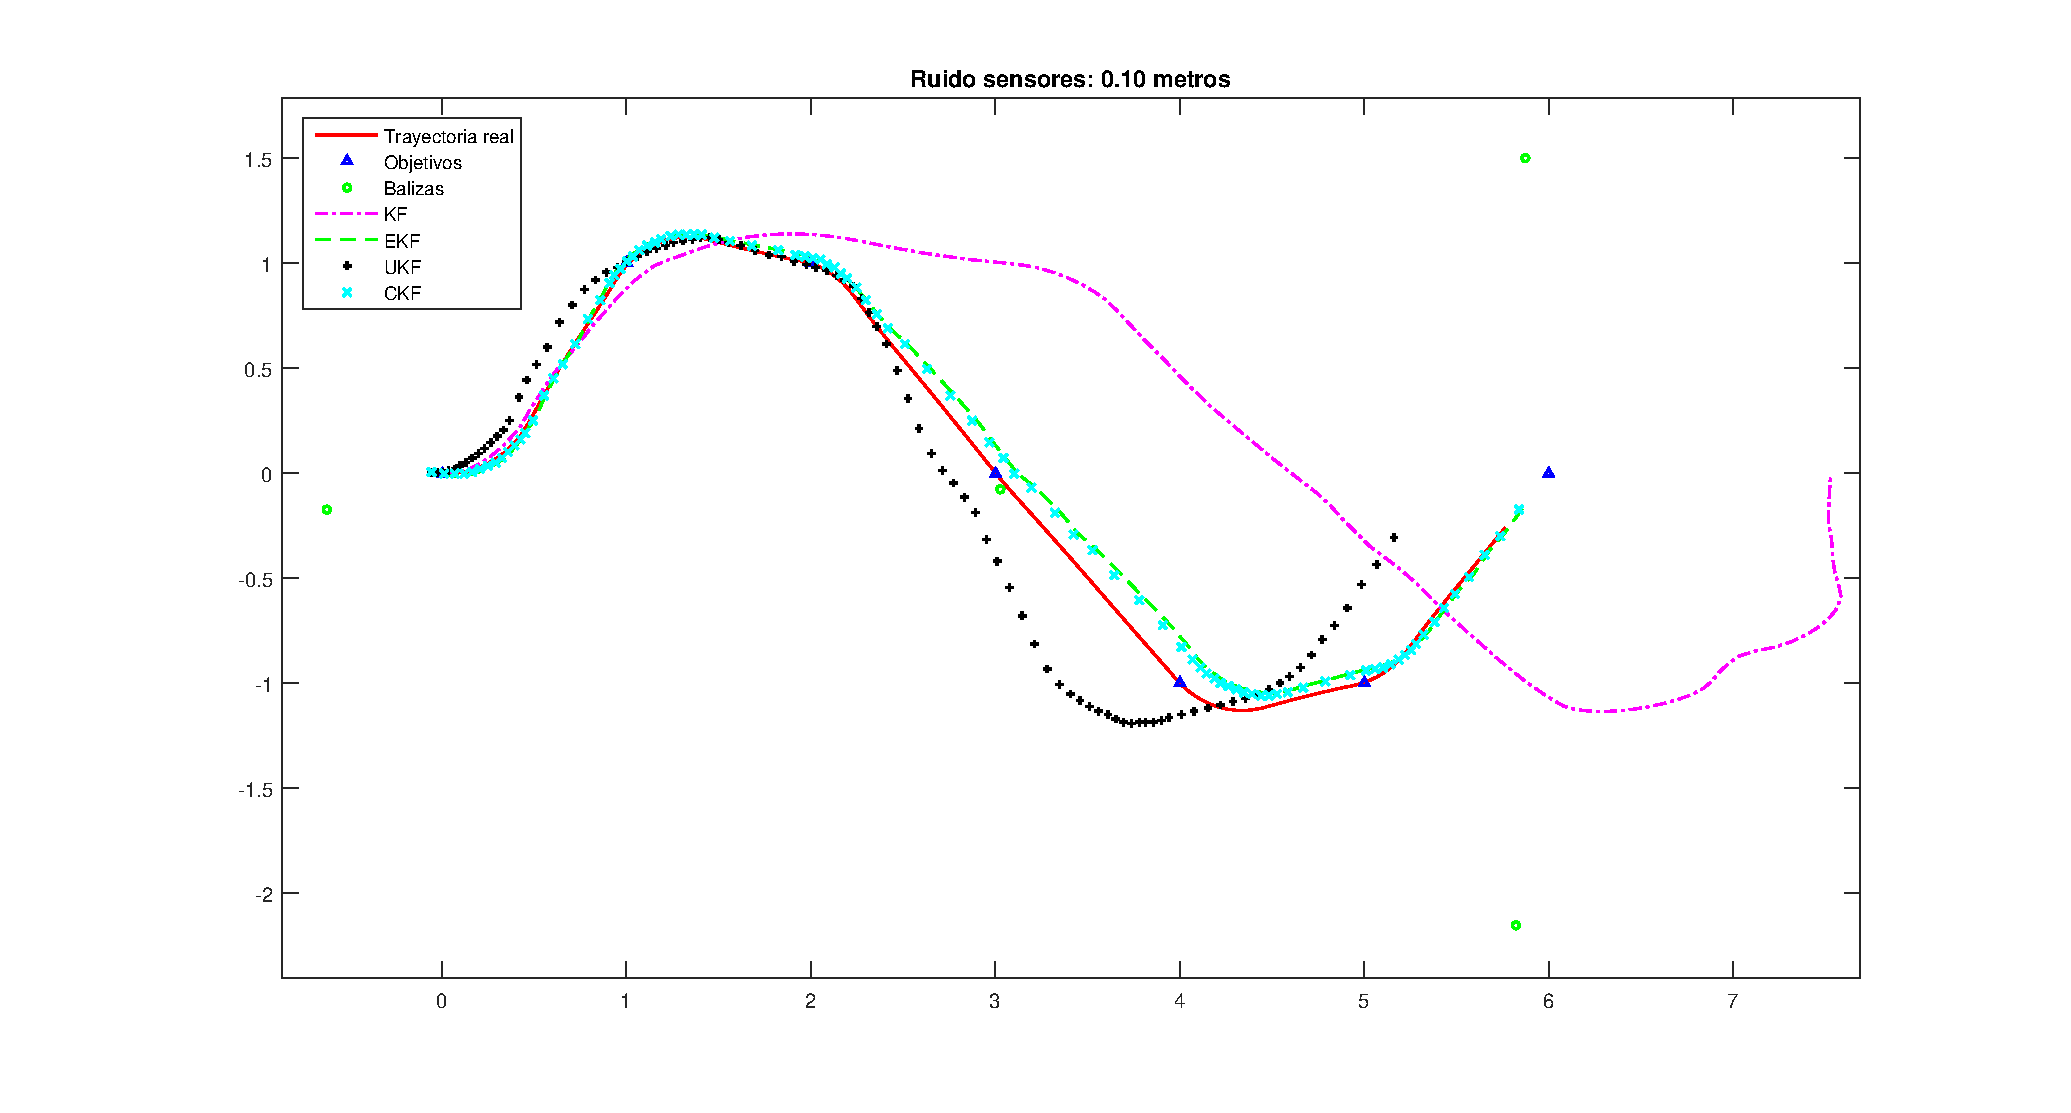
\includegraphics[scale=0.4]{Figura6}
\caption{Trayectoria senoidal función de medida de distancia} \label{Figura6}
\end{figure}

\begin{figure}[ht!]
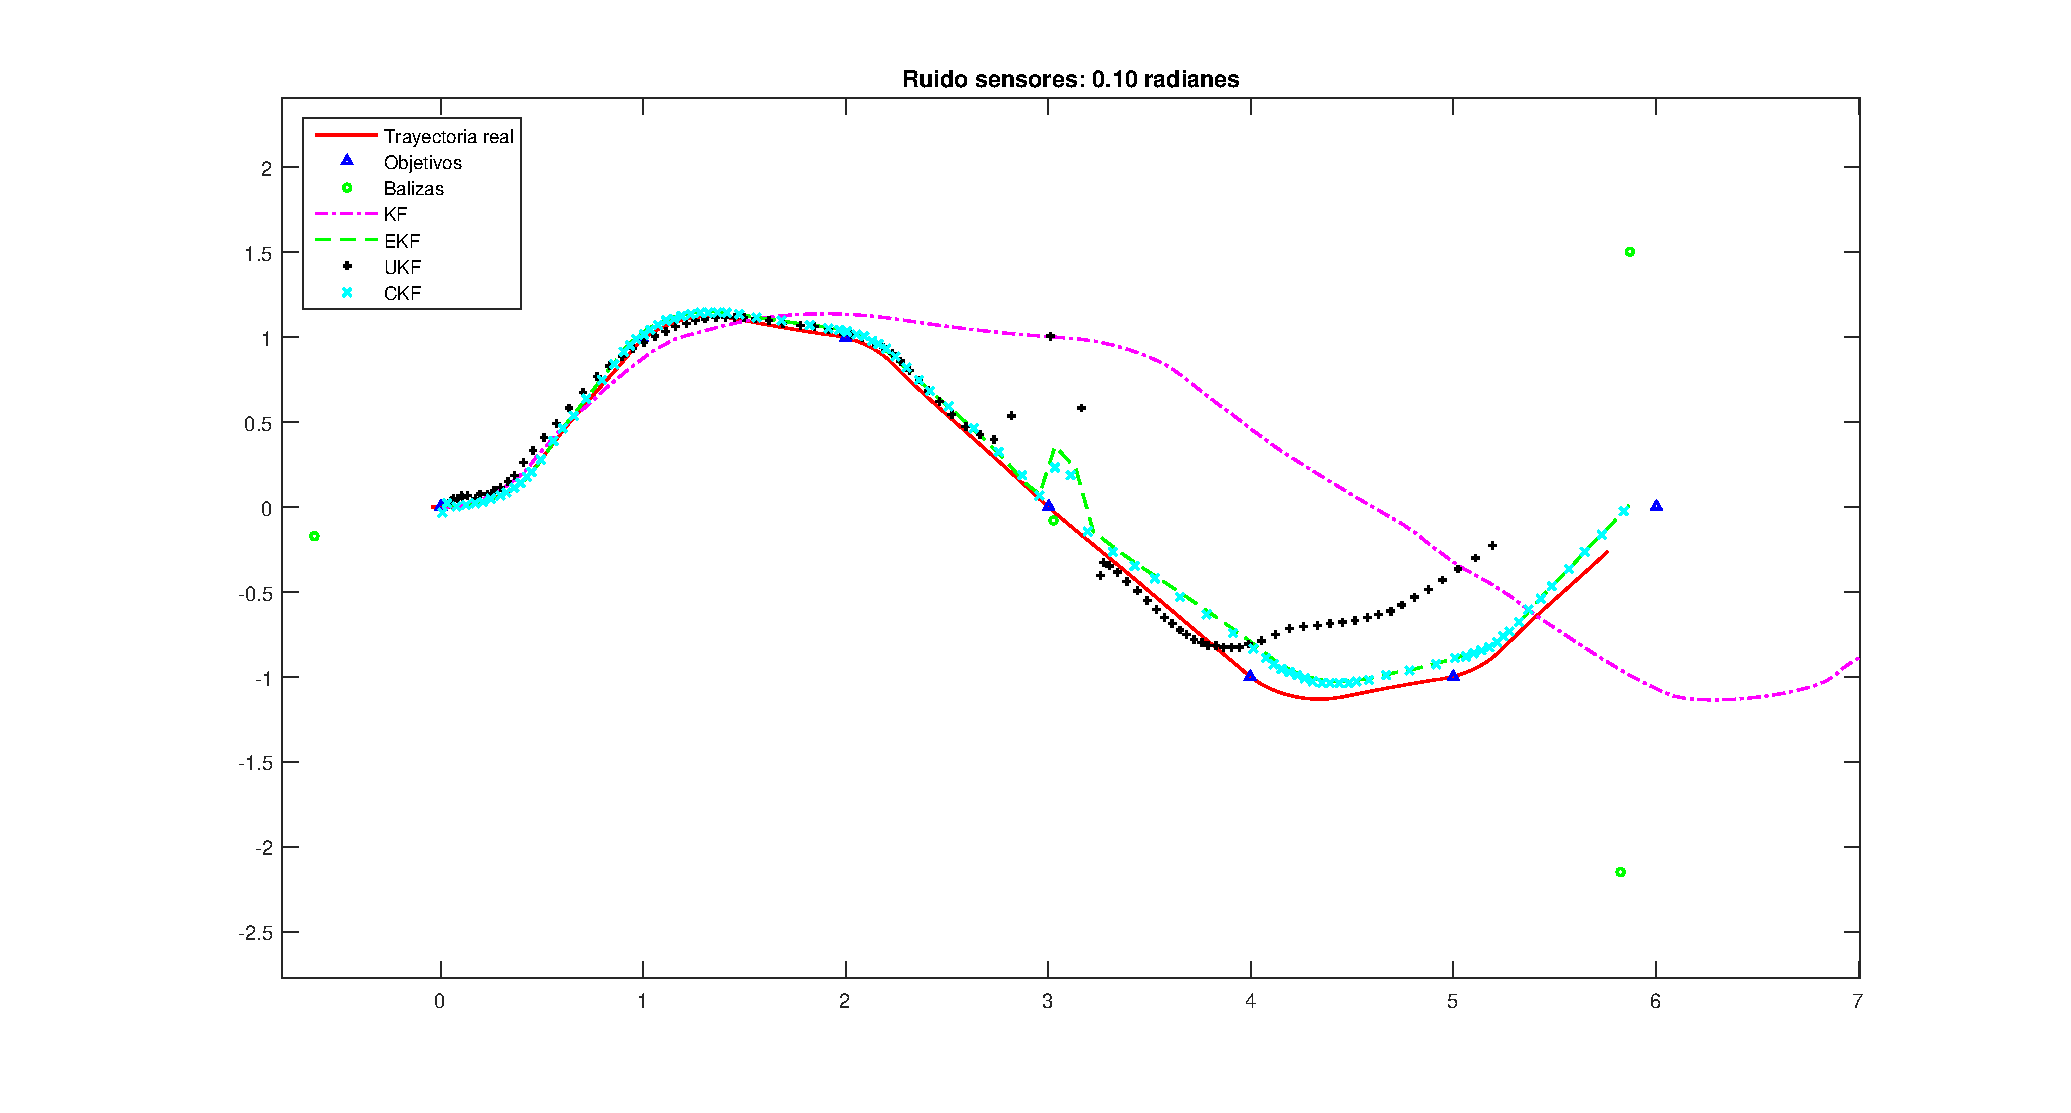
\includegraphics[scale=0.4]{Figura6_6}
\caption{Trayectoria senoidal función de medida de ángulos} \label{Figura6_6}
\end{figure}
Este experimento ha sido el único en el que el error cometido por el \ac{UKF} no ha sufrido variación en función del modelo de medida utilizado como podemos ver en las figuras \ref{Grafico6} y \ref{Grafico6_6}.
En esta prueba el filtro que ha presentado el menor error en general también ha sido el \ac{CKF}.
Por otro lado en este experimento vemos que los errores están muy cercanos entre sí, por lo que no hay gran diferencia entre usar un modelo de medida u otro.
Sin embargo, en la figura \ref{Figura6_6} vemos la singularidad que se ha producido en el \ac{EKF} y el \ac{CKF} esta clase de efectos hacen que la estimación empeore y por lo tanto la localización sea menos acertada.

La conclusión para esta serie de experimentos es la siguiente : \textbf{El error en la estimación aumenta a medida que aumenta el ruido presente en los sensores. El filtro que mejor se comporta ante este error es el \ac{CKF} ya que por lo general es el que menor error cuadrático medio presenta. Por último, el modelo de medida de ángulos presenta mayores errores que el de distancia, además presenta singularidades que empeoran la estimación por lo que es mejor el modelo de medida de distancias.}
% * <amorellg@ull.edu.es> 2016-06-06T20:32:34.967Z:
%
% > lidia
%
% se comporta ante
%
% ^ <alu0100765755@ull.edu.es> 2016-06-07T09:45:23.301Z.

\section{Experimentos 3: Variación del número de balizas}
En esta sección experimentaremos para ver cómo afecta cómo afecta tener información más rica para el sensor de balizas.
% * <amorellg@ull.edu.es> 2016-06-06T20:33:18.464Z:
%
% > implementar o no más información sensorial a nuestro robot.
%
% más bien: "cómo afecta tener información más rica para el sensor de balizas"
%
% ^ <alu0100765755@ull.edu.es> 2016-06-07T09:46:02.795Z.
El modelo de medida que usaremos será el de distancia (ecuación \ref{Modelo_distancia}) por ser el que menos error presenta.
% * <amorellg@ull.edu.es> 2016-06-06T20:34:57.574Z:
%
% > el más óptimo 
%
% quita esto, suena muy rimbombante
%
% ^ <alu0100765755@ull.edu.es> 2016-06-07T09:47:01.953Z.
Como hasta ahora, representaremos la información obtenida por medio de gráficos que facilitarán la comprensión de los datos.
Además representaremos las trayectorias seguidas por los filtros para el peor caso de estimación, que en el caso de esta serie de experimentos corresponde a la trayectoria con tres balizas disponibles.
\subsection{Resultados para la trayectoria recta}
Los resultados para estos experimentos se muestran en las figuras \ref{Grafico7} y \ref{Figura7}.
\begin{figure}[ht!]
\centering
\includegraphics[scale=0.6]{Grafico7}
\caption{Experimento recta variando número de balizas} \label{Grafico7}
\end{figure}
\begin{figure}[ht!]
\centering
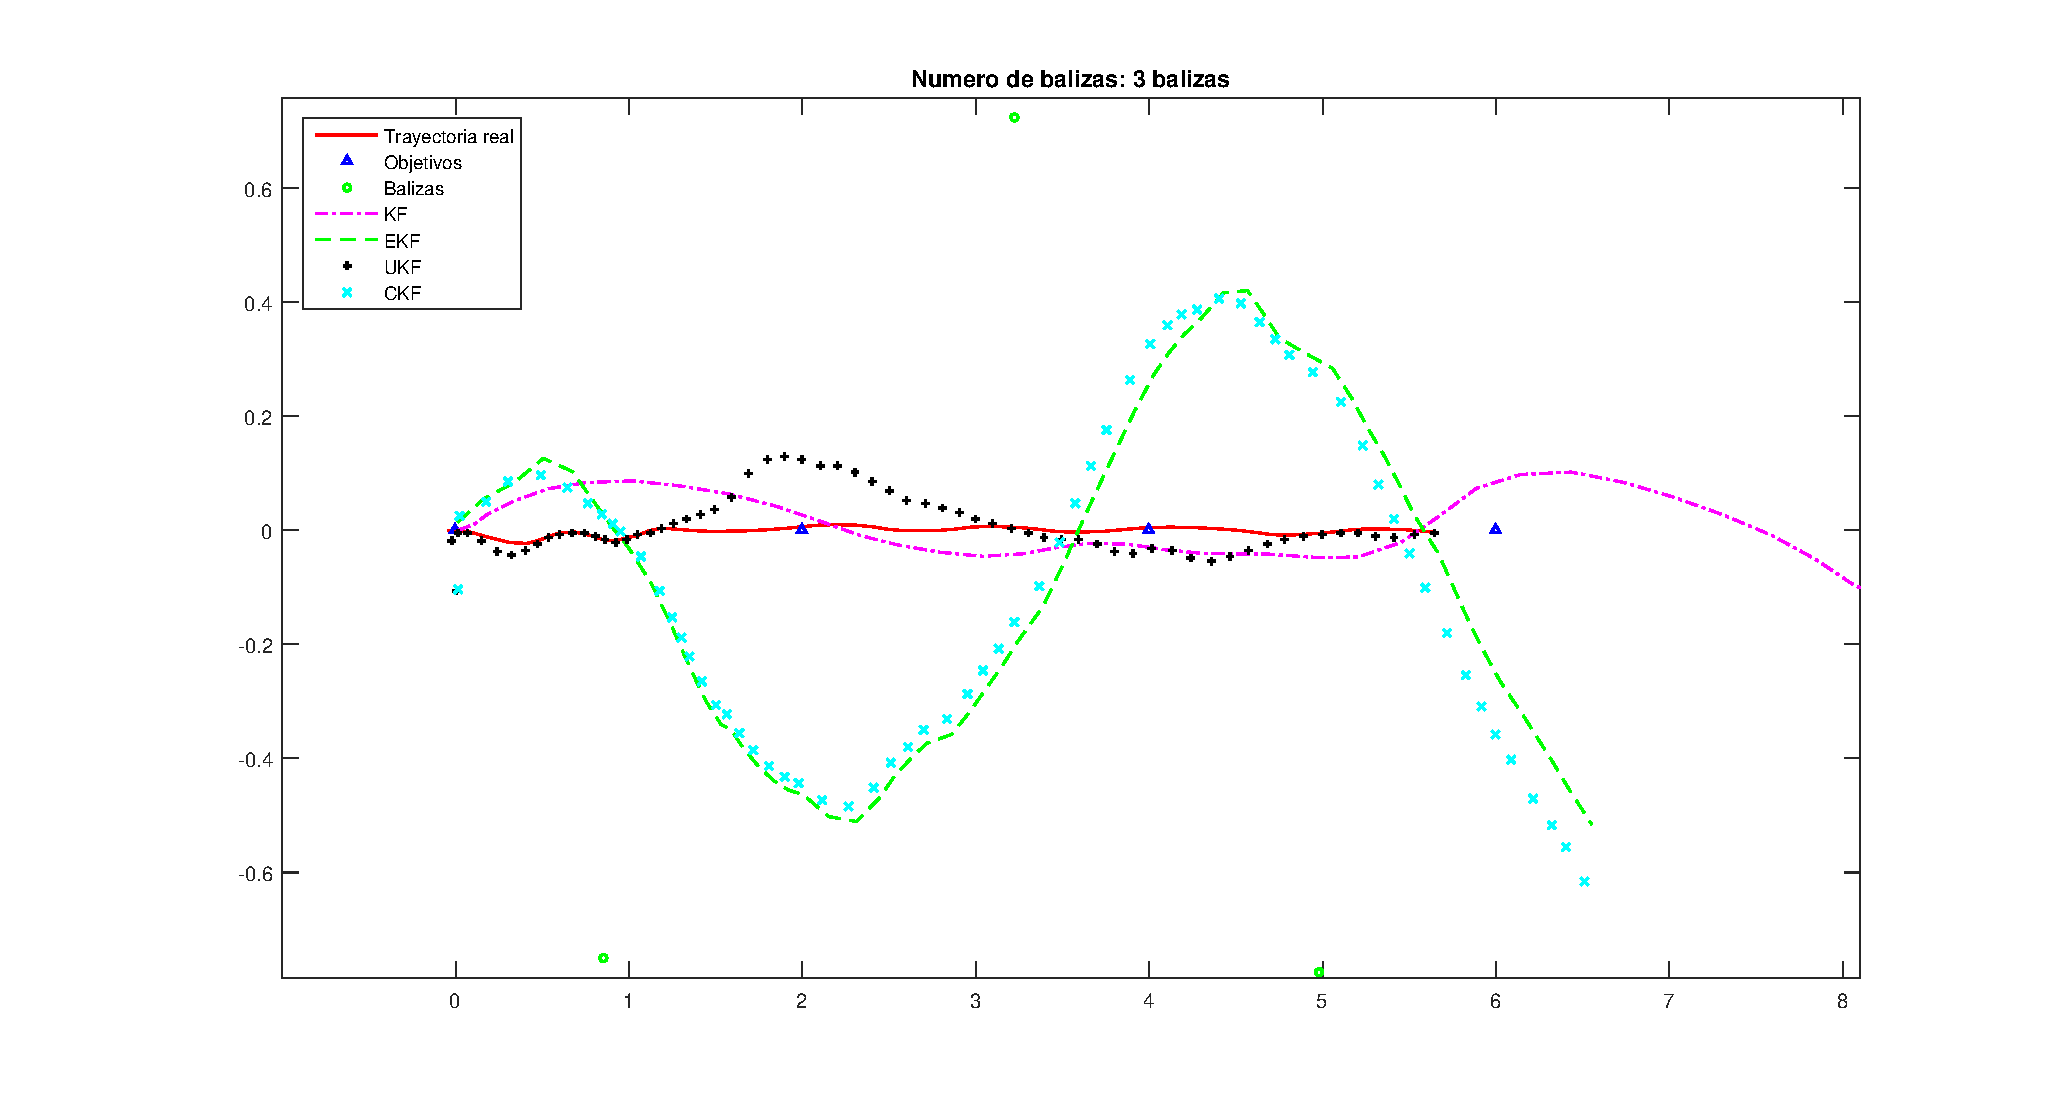
\includegraphics[scale=0.4]{Figura7}
\caption{Trayectoria recta 3 balizas} \label{Figura7}
\end{figure}
Vemos en la figura \ref{Grafico7} como el error disminuye a medida que aumentamos el número de balizas en la escena, lo cual es una de las premisas del filtro de Kalman , cuanta más información mejor estimación.
Además en la figura \ref{Figura7} podemos observar que cuando el \ac{EKF} y \ac{CKF} tienen poca información de las balizas, es decir tenemos pocas rodeando al robot, la estimación se vuelve totalmente errónea.
Por esta razón en la figura \ref{Figura7} vemos como se producen unas grandes oscilaciones en la estimación.
Hay que recordar que la trayectoria real mostrada en la figura difiere para cada una de las simulaciones de los filtros por lo que no hay que tomar esta como una referencia fiel de la realidad sino como una representación orientativa.

\subsection{Resultados para la trayectoria cuadrada}
Los resultados para esta serie de pruebas se muestran en las figuras .
\begin{figure}[ht!]
\centering
\includegraphics[scale=0.6]{Grafico8}
\caption{Experimento cuadrado variando número de balizas} \label{Grafico8}
\end{figure}
\begin{figure}[ht!]
\centering
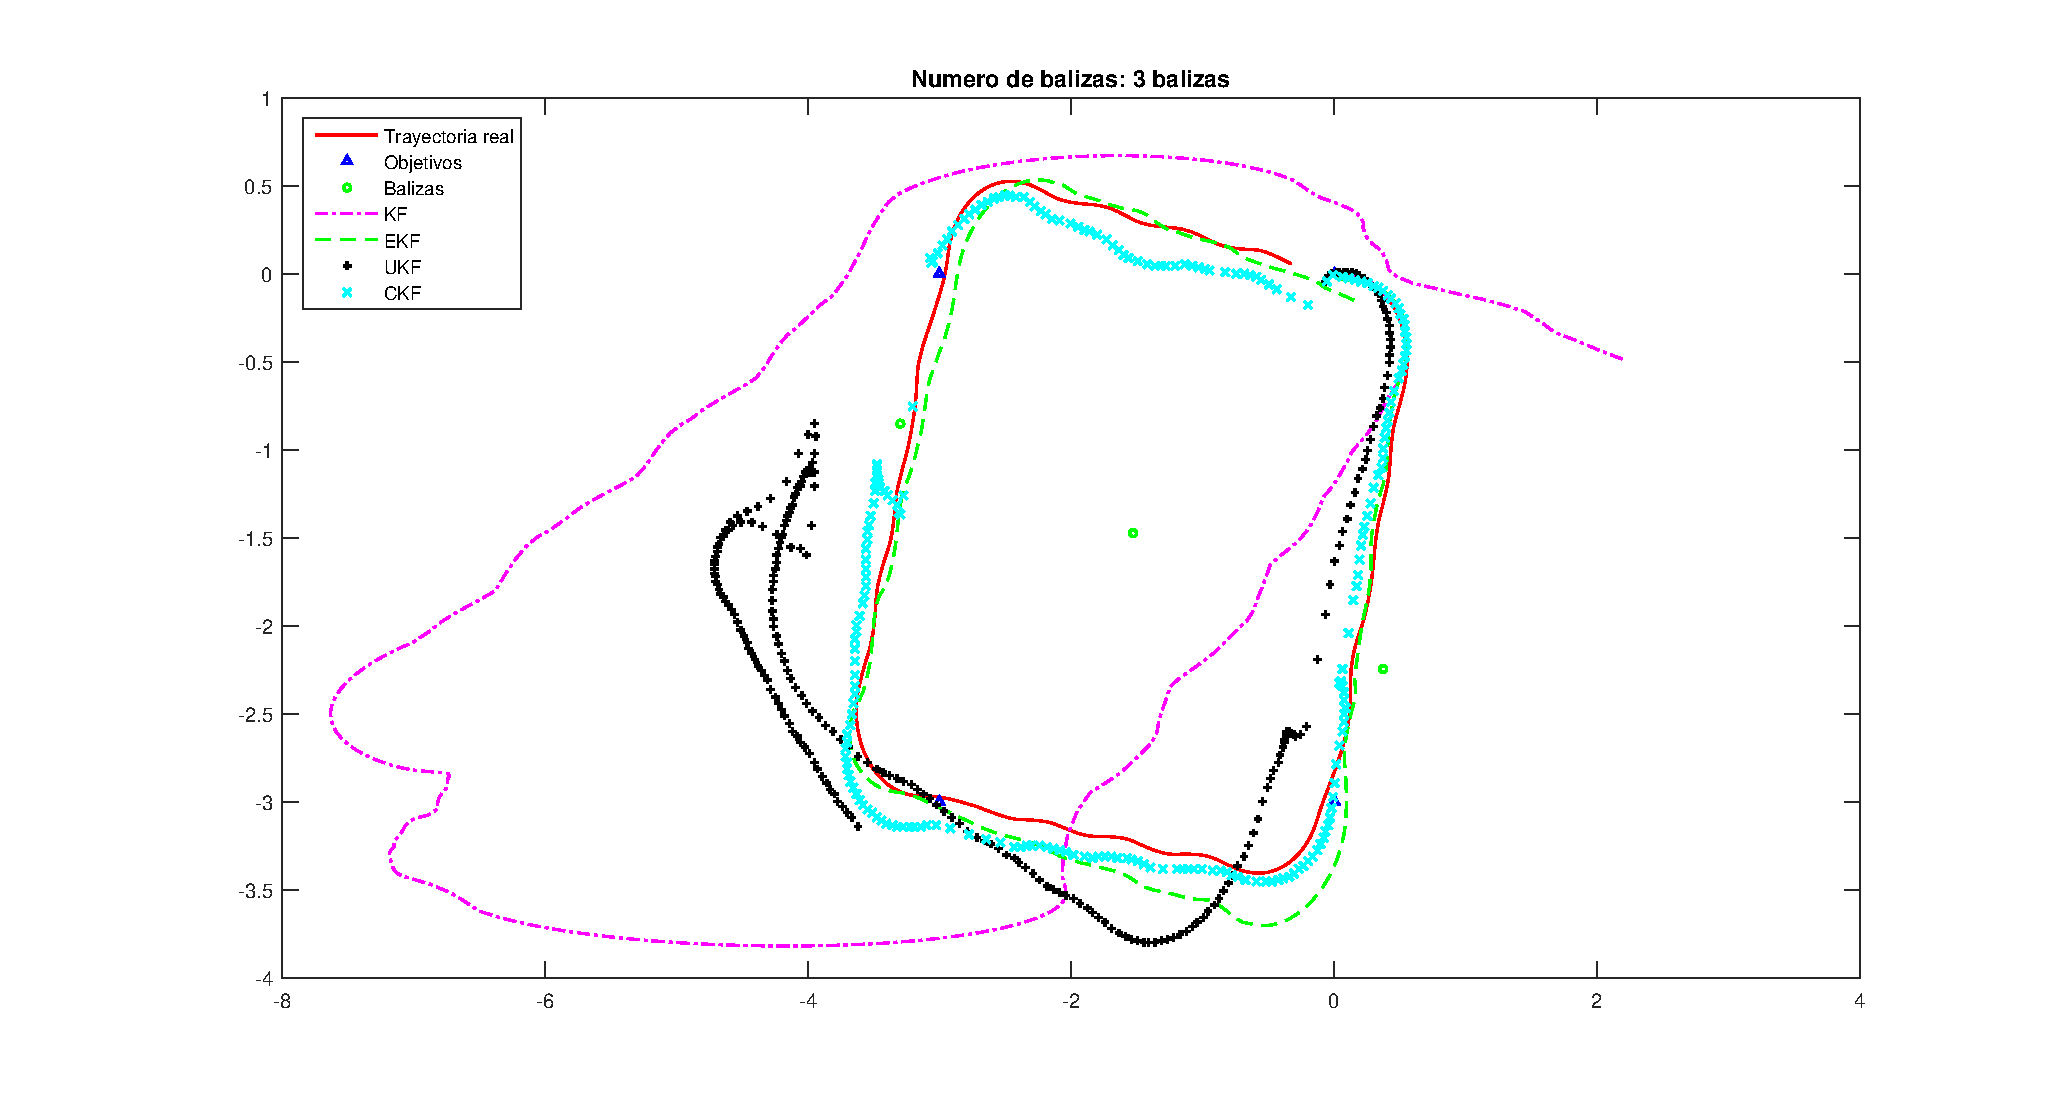
\includegraphics[scale=0.4]{Figura8}
\caption{Trayectoria cuadrada 3 balizas} \label{Figura8}
\end{figure}
Al igual que en el experimento anterior el error obtenido disminuye cuando aumentamos el número de balizas en la escena como vemos en la figura \ref{Grafico8}.
En este caso en la figura \ref{Figura8} podemos ver que el filtro de Kalman clásico presenta mucho error aunque este detalle no es relevante porque como ya hemos dicho la sintonización de este filtro no depende del número de balizas sino que depende únicamente de la odometría.
En esta figura, podemos ver como la estimación más acertada es la realizada por el \ac{CKF} y \ac{EKF} como también confirma la figura \ref{Grafico8}.

\subsection{Resultados para la trayectoria senoidal}
Los resultados de estas pruebas se muestran en las figuras \ref{Figura9} y \ref{Grafico9} .
\begin{figure}[ht!]
\centering
\includegraphics[scale=0.6]{Grafico9}
\caption{Experimento seno variando número de balizas} \label{Grafico9}
\end{figure}
\begin{figure}[ht!]
\centering
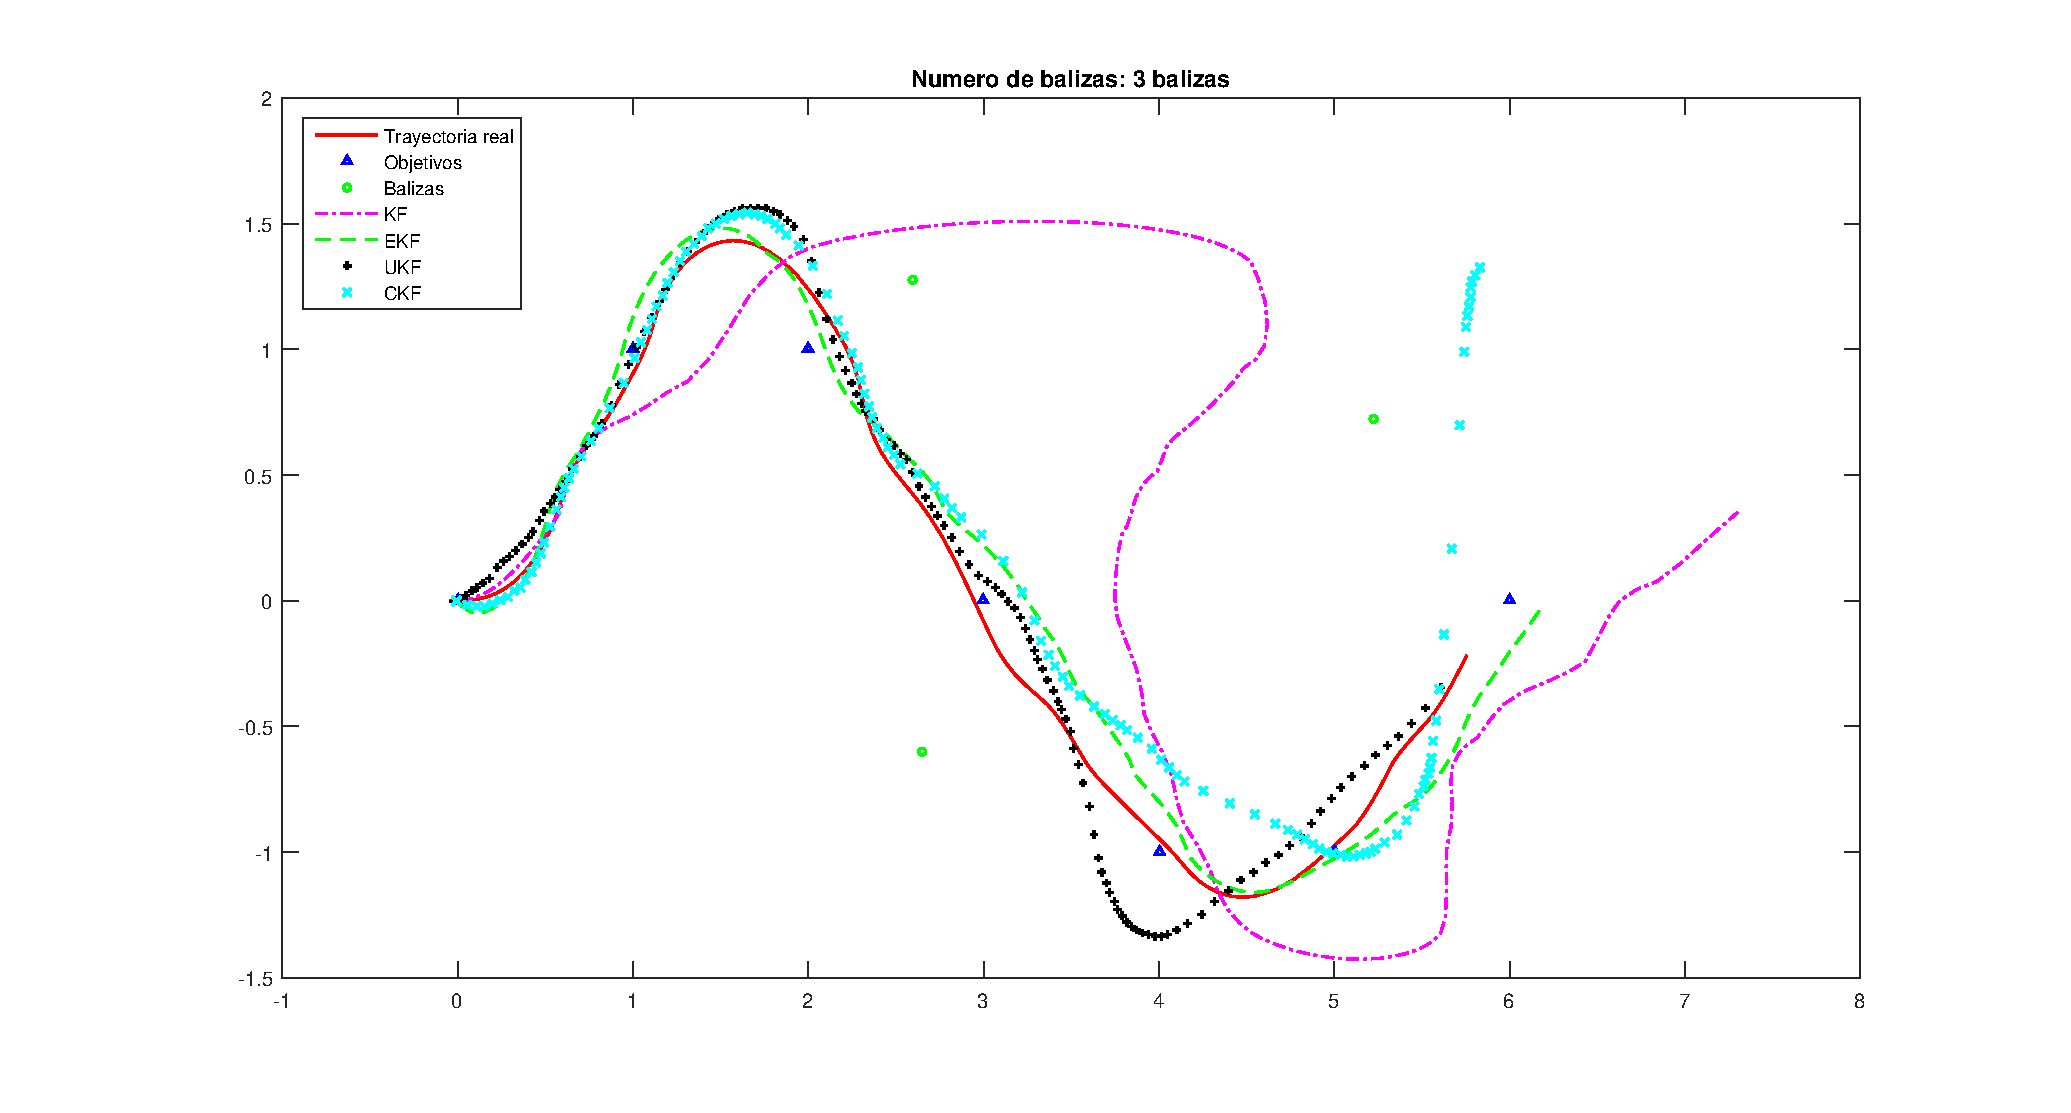
\includegraphics[scale=0.4]{Figura9}
\caption{Trayectoria senoidal 3 balizas} \label{Figura9}
\end{figure}
Para esta serie de experimentos el error entre filtros es bastante parecido.
Como vemos en la figura \ref{Grafico9} el error también disminuye a medida que aumentamos la información sensorial, lo que ha sido un punto en común entre todas las pruebas realizadas.
En la figura \ref{Figura9} podemos ver que las estimaciones de los filtros \ac{EKF}, \ac{UKF} y \ac{CKF} son muy parecidas entre sí.
También podemos observar este hecho en la figura \ref{Grafico9} donde vemos que los errores están próximos entre sí.

La conclusión para esta serie de experimentos es la siguiente : \textbf{El error en al estimación disminuye a medida que aumenta el número de balizas disponibles para tomar medidas. Los filtros por lo general se ven afectados en la misma medida por la falta de información sensorial. Si tuvieramos que destacar uno de ellos este sería el \ac{UKF} el cual tiende a aumentar mucho su error cuando la información sensorial es pobre por otra parte el \ac{CKF} es el que por lo general parece más robusto en cuanto a una disminución en la información sensorial.}
% * <amorellg@ull.edu.es> 2016-06-06T20:37:06.718Z:
%
% >  a la falta de información sensorial
%
% mejor: "a una disminución en la información sensorial"
%
% ^ <alu0100765755@ull.edu.es> 2016-06-07T09:47:48.130Z.

\section{Experimento 4: Rendimiento ante una trayectoria general}% * <amorellg@ull.edu.es> 2016-06-06T20:37:32.198Z:
%
% > Mejores condiciones de sintonización
%
% Rendimiento ante una trayectoria general
%
% ^ <alu0100765755@ull.edu.es> 2016-06-07T09:48:32.733Z.
En esta sección experimentaremos con la sintonización recomendada para los filtros para así  ver como se comporta cada uno en unas condiciones normalizadas de funcionamiento.
% * <amorellg@ull.edu.es> 2016-06-06T20:38:04.190Z:
%
% > a mejor sintonización
%
% sintonización recomendada
%
% ^ <alu0100765755@ull.edu.es> 2016-06-07T10:06:53.282Z.
Usaremos el modelo de medida de distancia para este experimento ya que es el más robusto.
Representaremos los resultados por medio de la tabla \ref{Exp_trayectoria_general} para ver cual ha sido el error para cada filtro además de mostrar en las figuras con  el resultado de la estimación para cada uno de los filtros utilizados.
Hay que tener en cuenta que las figuras seleccionadas son las que representan el peor caso en la estimación y lo realmente relevante son las medias obtenidas para los experimentos mostradas en la tabla \ref{Exp_trayectoria_general}.

\begin{table}[htbp]
\caption{Experimentos trayectoria general}
\begin{center}
\begin{tabular}{|l|c|c|l|c|c|c|c|}
\hline
\multicolumn{ 8}{|c|}{Experimento 4} \\ \hline
Recorrido & Deslizamiento & \multicolumn{ 2}{c|}{Ruido sensores (m)} & KF & EKF & UKF & CKF \\ \hline
Circuito  & 5,00\% & \multicolumn{ 2}{c|}{0,05} & 4.3& 1.4 & 1.355 &1.358 \\ \hline
\end{tabular}
\end{center}
\label{Exp_trayectoria_general}
\end{table}

\begin{figure}[ht!]
\centering
\includegraphics[scale=0.45]{Figura10_1}
\caption{Experimento trayectoria general EKF} \label{Figura10_1}
\end{figure}
\begin{figure}[ht!]
\centering
\includegraphics[scale=0.45]{Figura10_2}
\caption{Experimento trayectoria general UKF} \label{Figura10_2}
\end{figure}
\begin{figure}[ht!]
\centering
\includegraphics[scale=0.45]{Figura10_3}
\caption{Experimento trayectoria general CKF} \label{Figura10_3}
\end{figure}
 Podemos ver en la tabla \ref{Exp_trayectoria_general} que el filtro que ha obtenido el menor error en su estimación ha sido el \ac{UKF} seguido muy de cerca por el \ac{CKF}.
 En las figuras \ref{Figura10_1}, \ref{Figura10_2} y \ref{Figura10_3} podemos apreciar las diferencias entre las trayectorias debido al deslizamiento existente, ya que hace que la odometría de una información que hace imprecisa la estimación.
 Como vemos en la comparación de estas figuras, la estimación de los filtros es muy parecida, por lo que se ven afectados en la misma media por el deslizamiento.
% * <amorellg@ull.edu.es> 2016-06-06T20:53:58.958Z:
%
% > Es difícil llegar a saber cual es el mejor filtro en esta prueba ya que la colocación de las balizas, los deslizamientos y algunos otros factores pueden llegar a jugar un papel crucial.
%
% esto es lo que te comenté que habría que cambiar, en la conclusión general de este experimento sí se debería poder comparar  el error que  tiene cada filtro para la misma trayectoria
%
% ^ <alu0100765755@ull.edu.es> 2016-06-07T10:09:28.837Z.
 Podemos decir es que el \ac{UKF} ha sido el filtro que ha realizado la mejor estimación, aunque con muy poca diferencia sobre los demás como podemos ver en la tabla \ref{Exp_trayectoria_general} y la figura \ref{Figura10_2}.
 Por otra parte,como hemos dicho, en todos los filtros hemos implementado la odometría por lo que quizás de no haber implementado esta información sensorial la estimación podría haber cambiado.
 Aunque lo anterior fuera posible, el objetivo de esta prueba es testear los filtros en una situación en la que estén configurados de manera que incluyan la fusión sensorial.
 
La conclusión para esta serie de experimentos es la siguiente : \textbf{El \ac{UKF} ha sido el mejor adaptado a la trayectoria pero esto no quiere decir que sea el mejor filtro, como vemos los deslizamientos han generado que las trayectorias estimadas son bastante diferentes a las trayectorias reales debido a este motivo. Podemos concluir con este experimento que los deslizamientos pueden provocar muy malos resultados en la estimación  y aunque el \ac{UKF} muestre los mejores resultados el resto de filtros obtienen una estimación parecida. Sin embargo, el \ac{UKF} parece el que mejor se adapta a una trayectoria con deslizamientos. }

\section{Resultados generales}

Una vez hemos realizado todos los experimentos, tenemos que llegar a una conclusión global sobre todas la implementaciones que hemos hecho y sobre todo debemos sacar conclusiones acerca de los resultados obtenidos para las pruebas. 
Para facilitar la toma de decisiones hemos decidido dar una puntuación a la posición que ha obtenido cada filtro en la realización de los experimentos.
De esta manera estableceremos un ranking en el que posicionaremos cada uno de estos en orden y veremos como de cerca están unos de otros y además este nos permitirá tomar una decisión mucho más objetiva al respecto.
Las puntuaciones las hemos asignado en función de la posición obtenida en la realización del experimento, es decir, si por ejemplo el \ac{EKF} resulta hacer la mejor estimación en un experimento concreto se le sumarán 4 puntos, si es el segundo mejor se le sumarán 3 y así hasta llegar a 1 punto que corresponderá al filtro que quede en cuarto lugar.
Podemos ver en la tabla \ref{Tabla_puntuaciones} las puntuaciones obtenidas.
\begin{table}[htbp]
\caption{Puntuaciones obtenidas por los filtros}
\begin{center}
\begin{tabular}{|c|c|c|c|c|}
\hline
Experimento & \textbf{KF} & \textbf{EKF} & \textbf{UKF} & \textbf{CKF} \\ \hline
1 & 1 & 2 & 4 & 3 \\ \hline
2 & 1 & 2 & 3 & 4 \\ \hline
3 & 1 & 2 & 4 & 3 \\ \hline
4 & 1 & 4 & 2 & 3 \\ \hline
5 & 1 & 2 & 4 & 3 \\ \hline
6 & 1 & 2 & 4 & 3 \\ \hline
7 & 1 & 3 & 2 & 4 \\ \hline
8 & 1 & 2 & 4 & 3 \\ \hline
9 & 1 & 3 & 2 & 4 \\ \hline
10 & 1 & 4 & 2 & 3 \\ \hline
11 & 1 & 3 & 2 & 4 \\ \hline
12 & 1 & 3 & 2 & 4 \\ \hline
13 & 1 & 2 & 4 & 3 \\ \hline
14 & 1 & 4 & 2 & 3 \\ \hline
15 & 1 & 3 & 2 & 4 \\ \hline
16 & 1 & 2 & 4 & 3 \\ \hline
\textbf{TOTAL} & \textbf{\textit{16}} & \textbf{\textit{43}} & \textbf{\textit{47}} & \textbf{\textit{54}} \\ \hline
\end{tabular}
\end{center}
\label{Tabla_puntuaciones}
\end{table}



Como podemos observar el filtro que ha resultado tener el mejor desempeño general en todas la pruebas realizadas ha sido el \ac{CKF} lo cual no es una sorpresa si pensamos que este filtro es una de las últimas modificaciones ideadas para el filtro de Kalman clásico y por lo tanto su funcionamiento se supone más óptimo.
En segundo lugar tenemos al \ac{UKF}, este ha quedado en esta posición debido muy probablemente a su poca robustez a la hora de trabajar con distintas funciones de medida y con poca información sensorial lo cual provoca que realice malas estimaciones.
Por otro lado el \ac{UKF} suele mostrarse muy robusto cuando trabaja con trayectorias en las que se sufren deslizamientos.
Al \ac{UKF} lo sigue  el \ac{EKF} que en casi todos los experimentos se ha mantenido en la mitad de la clasificación, no es un filtro que haya destacado en nada positivamente pero tampoco lo ha hecho de manera negativa.
En último lugar se encuentra el \ac{KF} que como era de esperar sería el filtro que presentaría los peores resultados de los cuatro estudiados.
Sin embargo, en las implementaciones que hemos realizado sobre el \ac{KF} hemos visto que aunque su estimación es peor que en el caso de los otros tres filtros esta no suele cometer errores demasiado acusados cuando el deslizamiento es bajo.
Por contra, como vimos en el experimento de la trayectoria completa, si el deslizamiento es grande la estimación del \ac{KF} es totalmente errónea, comentiendo así un error inevitable para esta implementación del filtro.

%\acresetall

%%
%% conclusiones.tex - Memoria de la tesis
%%
%%   Copyright 2009-2010 Jesús Torres <jmtorres@ull.es>
%%
%% Esta obra está bajo licencia Creative Commons Reconocimiento 3.0 Unported
%%
\pagestyle{scrheadings}
\ihead[]{\rightmark}
\ohead[]{Iván Rodríguez Méndez}
\ofoot[]{\thepage{}}
\addchap{Conclusions and future work}
In this project we have developed a prototyping and simulation framework based on V-REP and MATLAB, which has demonstrated being a suitable combination of a dynamic robot simulator with a fast prototyping experimental environment.
By using a toolbox with both well--known and state--of--the--art implementations of Kalman filter algorithms~\cite{toolbox_simo}, as introduced in chapter~\ref{ch:capitulo3}, we were able to focus on designing and developing an experimental framework.
Using such framework we conducted some experiments to assess the impact of different key concepts related with mobile robot localization, and the issues that classic and novel Kalman filter algorithms suffer.

Regarding the experiments, we have observed that the algorithm showing a better performance on average was the \ac{CKF}, which has demonstrated being a state--of--the--art approach as shown in~\cite{zhang_cubature_2013}.
Furthermore, we have found that \ac{UKF} is a very strong method in many situations, but with a big weakness regarding the singularities which appear with poor information from sensors.
The \ac{EKF} has also proven to be a filter with a decent behavior, and while not standing out over the others, its performance tend to be enough for most situations.
Finally, the \ac{KF} was the filter with the worst performance of the four algorithms studied, as expected.
However, after the experiments conducted, we have seen that even if its estimates are worse that the ones of the other three filters, its performance is not too bad on situations with low slippery degree.
On the contrary, as we saw in the experiment on a complex path, if the slippery degree is large, the estimation of the \ac{KF} becomes totally wrong.

Although experiments have brought us some expected results, they have shed light on the actual version of the filter which would yield the best results, depending on the system we want to use with.
We have seen that Gaussian filters and especially Kalman filters are very sensitive to modeling errors.
For this reason, depending on the actual system which we are working with, we should apply a filter over others.
It is clear that if our system is very simple, where an \ac{EKF} would be enough, we should not waste resources trying to implement an \ac{UKF} or an \ac{CKF}.
On the other hand, if we have a real system with high nonlinearities or a large number of states, the most suitable implementation seems to be the \ac{CKF}.

For the \ac{CKF} and the \ac{UKF} we have proposed in chapter~\ref{ch:capitulo5} a modification on the odometry model.
As we have seen in the experiments, the implementation of these modifications has been a success since filters have obtained lower error in the estimation.

Thus, as the final conclusions, firstly, the application of any of these state--of--the--art filters (\ac{EKF}, \ac{UKF} and \ac{CKF}) depends on the complexity of our system, the modelization error of the disturbances, and the computational resources available.
Secondly, the toolbox used in this project has shown to be a great starting point for implementing localization experiments for mobile robots using the Kalman filtering theory.
Finally, the framework we have developed could be helpful for deploying simulated and real experiments to compare the algorithms described with other advanced localization algorithms, which could also be used for teaching purposes.
The resulting software has been published as a public repository on GitHub~\cite{_tfg_repo}.

\addsec{Future work}

It is obvious that using a simulator like V-REP eases the implementation.
However, there are many possible improvements regarding the implementation of the functions, as for example the memory allocation to gain speed in executing some parts of the code.
Furthermore, a faster implementation of the interaction with the simulator can be done in another programming language such as C++, Java, or Python, keeping the portability between different platforms.
Another interesting point to invest additional efforts could be the development of a graphical interface in which simulation parameters can be tuned.
Also, an improved representation of the results can be explored.

We could also consider the possibility of generating the position's objectives automatically, i.e. a random generator of each target.
A simillar implementation for the landmark placement could be done.

From the model point of view, the API supports importing any type of model and the modification of its physical properties, e.g., the size of the wheels or the frame of the robot.

As we can see, there is much work ahead on this project, which can also deploy advanced methods like particle filters and many more algorithms for estimating the position of a mobile robot.
The main idea after studying and implementing this Kalman filtering experimental framework is to allow for a platform which could be extended and become a tool to simulate different solutions to the problem of dynamic state estimation.



\appendix
%%
%% apendiceA.tex - Memoria de la tesis
%%
%%   Copyright 2009-2010 Jesús Torres <jmtorres@ull.es>
%%
%% Esta obra está bajo licencia Creative Commons Reconocimiento 3.0 Unported
%%
\pagestyle{scrheadings}
\ihead[]{\rightmark}
\ohead[]{Iván Rodríguez Méndez}
\ofoot[]{\thepage{}}
\chapter{Conceptos matemáticos para comprender el filtro de Kalman.}\label{ApendiceA}

Para caracterizar el filtro de Kalman es necesario tener claras una serie de ideas o mejor dicho, conceptos matemáticos. 
Aunque el filtro tiene un desarrollo teórico-matemático bastante extenso nos quedaremos únicamente con las partes más básicas que nos ayudarán a comprender el funcionamiento es este en esencia. 
Para tener un trasfondo contrastado con respecto a las explicaciones teóricas, hemos usado varias referencias \cite{Matematicas2004},\cite{Matematicasaplicadas2005},\cite{AnIntroductionToTheKalmanFilter} y \cite{IntroduccionMatematicaKalman}. En todos ellos se introducen los conceptos matemáticos de los que hablamos.

\section{Probabilidad de un evento.}

La mayoría de nosotros tenemos alguna noción o idea de lo que significa un evento aleatorio, o la probabilidad de que un evento pueda ocurrir en un espacio experimental.
Un experimento aleatorio se define como un experimento cuyo resultado es incierto, pero que se puede repetir (como podría ser el lanzamiento de un dado y que salga un número concreto). 
El conjunto de todos los posibles resultados de un experimento aleatorio se denomina espacio muestral, y se denomina a menudo con la siguiente notación $\Omega$. 
Formalmente, el resultado para la probabilidad de un evento discreto (por ejemplo el lanzamiento de una moneda) a favor está definida de la siguiente manera \ref{probabilidaddeunevento} :

\begin{equation}\label{probabilidaddeunevento}
p(A) = \frac{\textrm{Posibles  resultados  favorables  del  evento  A}}{\textrm{Número de todos los posibles resultados}}
\end{equation}

En el caso de eventos dependientes la probabilidad de que ocurra A o B está dada por \ref{probabilidadeventosdependientes}. 
Esta expresión también se conoce como la unión de A y B (se lee <<A unión B>>). Una representación clara de lo que implica la unión puede verse en la figura \ref{AunionB}.

\begin{equation}\label{probabilidadeventosdependientes}
p(A \cup B) = p(A) + p(B)
\end{equation}

\begin{figure}[H]
\centering
\includegraphics[width=0.3\textwidth]{AunionB}
\caption{Diagrama de Venn de A unión B.} \label{AunionB}
\end{figure}

Si la probabilidad de dos resultados es independiente, es decir que no afecta la una a la otra, entonces la probabilidad de que ambos ocurran está dada por \ref{probabilidadeventosindependientes}.
Esta operación se define como intersección de A y B (se lee <<A intersección B>>) Un ejemplo claro de intersección es el lanzamiento de dos monedas.
La probabilidad en un lanzamiento de que salga cara es de 1/2, por lo tanto la probabilidad de que en las dos monedas salgan cara al mismo tiempo es de 1/4 (claramente los resultados no se afectan entre sí ya que el resultado en uno de los lanzamientos no condiciona para nada al segundo de ellos)

\begin{equation}\label{probabilidadeventosindependientes}
p(A \cap B) = p(A) \cdot p(B)
\end{equation}

\begin{figure}[H]
\centering
\includegraphics[width=0.3\textwidth]{AinterseccionB}
\caption{Diagrama de Venn de A intersección B.} \label{AinterseccionB}
\end{figure}

Finalmente, si A y B son dos sucesos, la probabilidad de que ocurra B dado A (es decir que A ocurre antes que B) se denota por p(B $\mid$ A) y es llamada probabilidad condicional y viene dada por ~\ref{probabilidadcondicionada}.

\begin{equation}\label{probabilidadcondicionada}
p(A \mid B) = \frac{p(A \cap B)}{p(B)}
\end{equation}

\section{Variables Aleatorias.}

En contraposición a los eventos discretos, en un caso el seguimiento y la captura de movimiento, estamos más interesados en la aleatoriedad asociada a suceso como pueden ser la variación de una señal eléctrica o al movimiento de una persona (son eventos que se dan en un espacio continuo de tiempo).
En este caso podemos pensar en el elemento de interés como una variable aleatoria en un espacio continuo de valores como ya aclaramos anteriormente.
Una variable aleatoria es básicamente una función que mapea todos los puntos en el espacio de muestra a los números reales. 
Por ejemplo, la variable aleatoria continua $X(t)$ que podría mapear tiempo con respecto a posición, en cualquier instante de tiempo $t$ debería decirnos la posición esperada en dicho instante de tiempo.
Las variables aleatorias pueden ser discretas, cuando se puede contar el conjunto de los resultados posibles, o continuas, cuando toma valores en una escala continua lo que significa que el número de resultados posibles es infinito.

Una definición más formal de todo lo enunciado anteriormente, es que una variable aleatoria es una función del espacio muestral $\Omega$ en el conjunto de los números reales.
Las variables aleatorias se denominan generalmente X, Y, Z o con otra letra mayúscula escogida del del final del alfabeto. Por ejemplo, 

\begin{center}
\centering
X:$\Omega$ $\to$ R
\end{center}

define la variable aleatoria X como una función del espacio muestral en el conjunto de los números reales.

Las variables aleatorias se clasifican de acuerdo a su recorrido.
Si el número de valores que puede tomar es finito o infinito numerable (tiene infinitos elementos que pueden ser numerados, como el conjunto de números enteros), X se denomina variable aleatoria discreta. 
Si el recorrido de X es en un conjunto de valores (por ejemplo, los valores de un intervalo de números reales), se denomina variable aleatoria continua.

En el caso de variables aleatorias continuas, la probabilidad de cualquier evento simple discreto A es cero, esto es, P(A)=0.
Una función común que representa la probabilidad de una variable aleatoria, es definida como la función de distribución acumulativa.
Esta función (ecuación \ref{funciondistribucionacumulativa}) representa la probabilidad acumulativa de las variables aleatorias continuas X para todos (los no numerables) eventos hasta x.

\begin{equation}\label{funciondistribucionacumulativa}
F_{x}(x)= p(-\infty,x]
\end{equation}

Algunas importantes características de las funciones de distribución acumulativa son:

\begin{equation}\label{0cuandoxmenosinfinito}
F_{x}(x) \to \textrm{0 cuando x} \to -\infty
\end{equation}

\begin{equation}\label{1cuandoxmasinfinito}
F_{x}(x) \to \textrm{1 cuando x} \to +\infty
\end{equation}

\begin{equation}\label{funcionnodecreciente}
F_{x}(x) \textrm{es una función no decreciente de x} 
\end{equation}

la expresión \ref{funciondistribucionacumulativa} es usada más comúnmente en su forma de su derivada y se conoce como la función de densidad de probabilidad (ecuación \ref{funciondedensidaddeprobabilidad})

\begin{equation}\label{funciondedensidaddeprobabilidad}
f_{x}(x)=  \frac{\textrm{d}}{\textrm{dx}}F_{x}(x)
\end{equation}

La función de la expresión \ref{funciondedensidaddeprobabilidad} presenta las siguientes propiedades:

\begin{equation}\label{funciondensidaddeprobabilidadnonegativa}
f_{x}(x) \textrm{es una función no negativa} 
\end{equation}

\begin{equation}\label{probabilidaddelaintegraldensidaddeprobabilidad}
\int_{-\infty}^{+\infty}f_{x}(x)dx = 1  
\end{equation}

Finalmente la probabilidad en la integral en cualquier intervalo [a,b] está definida como:

\begin{equation}\label{integraldensidaddeprobabilidad}
P(a < X < b) = \int_{a}^{b}f_{x}(x)dx = P(X < b) - P(X < a)
\end{equation}

\section{Media y varianza.}

Al saber la distribución de una variable aleatoria tenemos un conocimiento total sobre ella. 
Sin embargo, en la práctica a menudo es imposible o innecesario conocer la distribución de probabilidad que describe un experimento aleatorio particular. 
En lugar de lo anterior, puede ser suficiente determinar unas pocas cantidades características, como el valor medio y una medida que describa la dispersión alrededor del valor medio (de esta forma se caracteriza en una distribución de probabilidad Normal). 
Muchos de nosotros estamos familiarizados con el concepto de media o promedio de un serie de números. 
La media para un espacio muestral N (se define como espacio muestral todos los posibles resultados de un experimento estadístico,como comentamos en la sección anterior) de una variable aleatoria X, el promedio, la media muestral o esperanza está dada por:

\begin{equation}\label{mediamuestral}
\bar{X} = \frac{X_{1} + X_{2} + \dots + X_{N}}{N}
\end{equation}

La media de una variable aleatoria X, se puede expresar como $\mu_{X}$ o simplemente como $\mu$ cuando sabemos a que variable aleatoria está referido. 
También es común referirse a la media como el valor esperado o esperanza, en cuyo caso se expresa como E(X).

Si X es una variable aleatoria discreta con distribución de probabilidad f(x) la media o valor esperado de X vendría dado de la siguiente forma:

\begin{equation}\label{mediavariablealeatoriadiscreta}
\mu = E(X) = \sum_{x}xf(x) 
\end{equation}

En el caso de que X sea una variable aleatoria continua tendríamos la siguiente expresión:

\begin{equation}\label{mediavariablealeatoriacontinua}
\mu = E(X) = \int_{-\infty}^{+\infty}xf(x) dx
\end{equation}

La varianza es un elemento de gran importancia que caracteriza la distribución de una variable aleatoria. 
Describe la amplitud del recorrido de la variable aleatoria. 
En otras palabras es un término que nos da información sobre la desviación o dispersión que hay con respecto a la media en las muestras usadas para calcular dicha media.
Un ejemplo para explicar el concepto de varianza podría el ruido en una señal senoidal, en este caso la varianza nos daría una idea de la afectación del ruido en dicha señal. 
Para cualquier variable aleatoria X de media $\mu$, la varianza $\sigma^2$ se define como:

\begin{equation}\label{varianza}
\sigma^2 = var(X) = E(X - \mu)^2
\end{equation}

En el caso de que X sea una variable aleatoria discreta, entonces la varianza sería:

\begin{equation}\label{varianzadiscreta}
\sigma^2 = var(X) = \sum_{x}(x-\mu)^2 f(x)
\end{equation}

Por otro lado en el caso de que X sea una variable aleatoria continua, la varianza se definiería de la siguiente manera:

\begin{equation}\label{varianzacontinua}
\sigma^2 = var(X) = \int_{-\infty}^{+\infty}(x-\mu)^2 f(x) dx
\end{equation}

En el caso de que X sea continua la raíz cuadrada de la varianza $\sqrt[]{\sigma^2} = \sigma $, se conoce como la desviación típica o estándar de X.

La varianza en una propiedad estadística muy usada en las señales aleatorias, ya que si se supiera la varianza de una señal que de otro modo fuera supuesta para ser constante alrededor de un valor, la magnitud de la varianza daría una idea de cuanto nos estamos desviando con respecto a la media.
En el filtro de Kalman usaremos la varianza con el fin de saber cuanto ruido hay en nuestra medida o como de deslocalizados nos encontramos en el mapa, este asunto lo trataremos en secciones posteriores cuando hablemos de la propagación del error.

\section{Distribución de probabilidad Normal o Gaussiana}
Esta distribución de probabilidad ha tenido un uso muy extendido en el modelado de sistemas aleatorios por muchas razones.
Introduciremos algunas de ellas para poder caracterizarla. 
Muchos procesos de la naturaleza podrían asemejarse a una distribución normal o estar muy cercana a esta, es decir que se comportan siguiendo una distribución de probabilidad que bien podría ser una normal.
De hecho, bajo unas condiciones concretas, se puede demostrar que una suma de variables aleatorias con cualquier distribución tiende hacia una distribución normal o de Gauss. 
El teorema que define esta propiedad es conocido como el teorema del límite central, y es muy útil para ciertas aplicaciones. 
La distribución Normal o Gaussiana que podemos ver en la figura \ref{distribucionnormal_figura} tiene algunas propiedades que la hacen matemáticamente muy manejable y es uno de los ejes principales sobre los que se postuló el filtro clásico de Kalman.

\begin{figure}[H]
\centering
\includegraphics[width=0.7\textwidth]{d_normal_4}
\caption{Función de distribución de probabilidad Normal o Gaussiana.} \label{distribucionnormal_figura}
\end{figure}

La función de densidad de probabilidad de una variable aleatoria X con distribución normal de parámetros $\mu$ y $\sigma$ se define matemáticamente como:

\begin{equation}\label{distribucionnormal}
f(x) = \frac{1}{\sigma\sqrt[]{2\pi}}e^{-(x-\mu)^2/2\sigma^2} , -\infty < x < \infty
\end{equation}

La notación típica para representar los valores de densidad de una variable aleatoria X con media $\mu$ y desviación típica $\sigma$ es $\dist{N}$(X;$\mu$,$\sigma$) aunque en algunos textos también se usa la varianza(no implica ningún problema ya que esta se deriva de la desviación típica). Algunas propiedades de la distribución normal son las siguientes:


1. f(x) es simétrica respecto a x = $\mu$.

2. El máximo de f(x) está en x = $\mu$.

3. Los puntos de inflexión de f(x) están en x = $\mu$ + $\sigma$ y x = $\mu$ - $\sigma$.

Como f(x) es una función de densidad cumple las siguientes propiedades:

\begin{equation}\label{distribucionnormalmayorquecero}
f(x) \geq 0
\end{equation}

\begin{equation}\label{distribucionnormalintegral1}
\int_{-\infty}^{+\infty}f(x)dx = 1
\end{equation}

\begin{equation}\label{distribucionnormalmediaintegral}
\mu = \int_{-\infty}^{+\infty}xf(x)dx
\end{equation}

\begin{equation}\label{distribucionnormalprobabilidad}
P(a \geq X \geq b) = \int_{a}^{b}\frac{1}{\sigma\sqrt[]{2\pi}}e^{-(x-\mu)^2/2\sigma^2}
\end{equation}

La propiedad de la ecuación \ref{distribucionnormalprobabilidad} se da si una cantidad X está normalmente distribuida con parámetros $\mu$ y $\sigma$, en caso contrario no se cumpliría la igualdad ya que no estaríamos tratando con una distribución de probabilidad gaussiana para la cual se define la expresión.

\section{Independencia y Probabilidad condicional}

Podemos ver que en las ecuaciones (\ref{AinterseccionB}) y \ref{probabilidadcondicionada}, que la probabilidad ha sido definida para variables aleatorias continuas. Dos variables aleatorias continuas X e Y son independientes estadísticamente si la probabilidad conjunta $f_{xy}(x,y)$ es igual a la suma de sus probabilidades marginales, es decir, que se consideran independientes si que cumple lo siguiente:

\begin{equation}\label{sucesosindependientes}
f_{xy}(x,y) = f_{x}(x)f_{y}(y)  \longrightarrow P(X \cap Y)
\end{equation}

Un ejemplo algo más claro para ilustrar la independencia sería suponer que lanzamos una moneda dos veces y que dicha moneda no está trucada. Sea A el suceso de que en el primer lanzamiento salga cara y B el suceso de que en el segundo lanzamiento salga cara. Supongamos que A ocurre ¿Cambia eso la probabilidad de que B ocurra?La respuesta lógica que todos daríamos es que no y efectivamente así es. Sabemos que el resultado del lanzamiento de la primera moneda no influye en el resultado del segundo lanzamiento. En el caso de que dos eventos se condicionen entre sí en el cálculo de la probabilidad (sacar bolas de colores de una bolsa) podríamos expresarla de forma matemática. Esta idea se puede expresar matemáticamente usando el concepto de probabilidad condicional que veíamos al principio de esta sección en la ecuación \ref{probabilidadcondicionada} donde expresaríamos la probabilidad de que un evento ocurra cuando previamente ha ocurrido otro.

Otro concepto muy relevante a la hora de hablar de probabilidad condicional es el teorema de Bayes. Para ilustrar la motivación de esta expresión nos remitiremos a un ejemplo expuesto en \cite{Matematicas2004}. Imaginemos que calculamos la probabilidad de que el resultado de un test de VIH realizado sobre un individuo escogido aleatoriamente sea positivo. Para el individuo, es mucho más importante saber si el resultado positivo del test realmente significa que está infectado por el virus. Las probabilidades estaban definidas de la siguiente manera:

\hspace{3.7cm}A = El resultado del test es positivo.

\hspace{3.7cm}$B_1$ = La persona está infectada.

\hspace{3.7cm}$B_2$ = La persona no está infectada.

Estamos interesados en P($B_1$$\mid$ A), es decir, la probabilidad de que una persona esté infectada sabiendo que el resultado es positivo. Las probabilidades P(A$\mid$ $B_1$) y P(A$\mid$ $B_2$) se deducen directamente de las características del test. Ahora queremos calcular las probabilidades condicionales cuando los papeles de A y $B_1$ se invierten.

Antes de calcular la probabilidad en este ejemplo específico, consideraremos el caso más general. Supongamos que los conjuntos $B_1$,$B_2$,$\dots$,$B_n$ forman una partición del espacio muestral $\Omega$, A es un suceso y las probabilidades P(A $\mid$ $B_i$), donde i=1,2,$\dots$,n son conocidas. Lo que queremos calcular son las probabilidades P(A $\mid$ $B_i$). Para la realización del cálculo se procedería de la siguiente manera:

Utilizando la definición de probabilidades condicionales tenemos:

\begin{equation}\label{Pcondicionaejemplo}
P(B_i \mid A) = \frac{P(A \cap B_i)}{P(A)}
\end{equation}

Para calcular $P(A \cap B_i)$, ahora se condiciona sobre $B_i$ :

\begin{equation}\label{Pcondicionaejemplo2}
P(A \cap B_i) = P(A\mid B_{i})P(B_i)
\end{equation}

Por otro lado para evaluar el denominador P(A) se utiliza la ley de la probabilidad total:
\begin{equation}\label{Pcondicionaejemplo3}
P(A) = \sum_{j=1}^{n}P(A\mid B_{j})P(B_j)
\end{equation}

Combinando las expresiones ~\ref{Pcondicionaejemplo},~\ref{Pcondicionaejemplo2} y ~\ref{Pcondicionaejemplo3} se llega a la siguiente expresión, conocida como fórmula de Bayes o teorema de Bayes. Formalmente, siendo $B_{1}$,$B_{2}$,$\dots$,$B_n$ una partición de $\Omega$ y A un suceso. Entonces

\begin{equation}\label{Teoremadebayes}
P(B_{i}\mid A) = \frac{P(A \mid B_{i}P(B_{i}}{\sum_{j=1}^{n}P(A \mid B_{j})P(B_{j})}
\end{equation}

Volviendo al ejemplo, si deseamos calcular P($B_{1} \mid A$), que es la probabilidad de que una persona esté infectada dado un resultado positivo en el test. Una vez el test ha dado positivo la población se divide en dos conjuntos, uno denominado $B_{1}$ en el que la persona está infectada y otro $B_{2}$ en el que la persona no está infectada. Si usamos la expresión \ref{Teoremadebayes} que es el teorema de Bayes, tenemos:

\begin{equation}\label{Pcondicionaejemplo4}
P(B_{1}\mid A) = \frac{P(A \mid B_{1}P(B_{1}}{P(A \mid B_{1})P(B_{1}) + P(A \mid B_{2})P(B_{2})}
\end{equation}

De esta manera calcularíamos la probabilidad de que una persona se encuentre infectada sabiendo que el test ha resultado positivo.

Con todos estos conceptos ya tendríamos los suficientes conocimientos como para comprender la base matemática básica sobre la que se formulan los filtros Bayesianos y por supuesto los filtros de Kalman.
El resto de formulaciones matemáticas relacionadas con los filtros Bayesianos las encontraremos en el capítulo \ref{ch:capitulo2} junto con su explicación teórica.

\pagestyle{scrheadings}
\ihead[]{\rightmark}
\ohead[]{Iván Rodríguez Méndez}
\ofoot[]{\thepage{}}
\chapter{Toolbox utilizada en Matlab.}\label{ApendiceB}
Para la realización de este trabajo hemos utilizado una toolbox de MATLAB realizada por Jouni Hartikainen, Arno Solin y Simo Särkkä.
El objetivo de esta toolbox es implementar todas las funciones vistas en el capítulo \ref{ch:capitulo3} de este trabajo y muchas otras.
Para una mayor comprensión sobre la propia toolbox y los códigos que se presentan en algunos capítulos de este trabajo introduciremos las funciones que hemos utilizado (únicamente las básicas sobre los filtros), para ello introduciremos los segmentos de código de MATLAB con los parámetros de cada función explicados.
Todas aquellas que funciones que son llamadas dentro de la implementación de los filtros no las incluiremos en este apéndice ya que haría su lectura demasiado engorrosa.
Para encontrar más información acerca del resto de funciones puede consultarse \cite{toolbox_simo}, donde encontrarán la toolbox para su descarga además de su documentación.

\section{Filtro clásico de Kalman}
\subsection{Ciclo de predicción}
\lstset{language=Matlab, breaklines=true, basicstyle=\footnotesize}
\lstset{numbers=left, numberstyle=\tiny, stepnumber=1, numbersep=-2pt}
\begin{lstlisting}[frame=single]
 %KF_PREDICT  Perform Kalman Filter prediction step
% Syntax:
%   [X,P] = KF_PREDICT(X,P,A,Q,B,U)
% In:
%   X - Nx1 mean state estimate of previous step
%   P - NxN state covariance of previous step
%   A - Transition matrix of discrete model (optional, default identity)
%   Q - Process noise of discrete model (optional, default zero)
%   B - Input effect matrix (optional, default identity)
%   U - Constant input (optional, default empty)
%
% Out:
%   X - Predicted state mean
%   P - Predicted state covariance
% Description:
%   Perform Kalman Filter prediction step. The model is
%     x[k] = A*x[k-1] + B*u[k-1] + q,  q ~ N(0,Q).
%   The predicted state is distributed as follows:
%     p(x[k] | x[k-1]) = N(x[k] | A*x[k-1] + B*u[k-1], Q[k-1])
%   The predicted mean x-[k] and covariance P-[k] are calculated
%   with the following equations:
%     m-[k] = A*x[k-1] + B*u[k-1]
%     P-[k] = A*P[k-1]*A' + Q.
%   If there is no input u present then the first equation reduces to
%     m-[k] = A*x[k-1]
function [x,P] = kf_predict(x,P,A,Q,B,u)
  % Check arguments
  %
  if nargin < 3
    A = [];
  end
  if nargin < 4
    Q = [];
  end
  if nargin < 5
    B = [];
  end
  if nargin < 6
    u = [];
  end  
  %
  % Apply defaults
  %
  if isempty(A)
    A = eye(size(x,1));
  end
  if isempty(Q)
    Q = zeros(size(x,1));
  end
  if isempty(B) & ~isempty(u)
    B = eye(size(x,1),size(u,1));
  end
  %
  % Perform prediction
  %
  if isempty(u)
    x = A * x;
    P = A * P * A' + Q;
  else
    x = A * x + B * u;
    P = A * P * A' + Q;
  end

\end{lstlisting}

\subsection{Ciclo de actualización}
\lstset{language=Matlab, breaklines=true, basicstyle=\footnotesize}
\lstset{numbers=left, numberstyle=\tiny, stepnumber=1, numbersep=-2pt}
\begin{lstlisting}[frame=single]
%KF_UPDATE  Kalman Filter update step
% Syntax:
%   [X,P,K,IM,IS,LH] = KF_UPDATE(X,P,Y,H,R)
% In:
%   X - Nx1 mean state estimate after prediction step
%   P - NxN state covariance after prediction step
%   Y - Dx1 measurement vector.
%   H - Measurement matrix.
%   R - Measurement noise covariance.
% Out:
%   X  - Updated state mean
%   P  - Updated state covariance
%   K  - Computed Kalman gain
%   IM - Mean of predictive distribution of Y
%   IS - Covariance or predictive mean of Y
%   LH - Predictive probability (likelihood) of measurement. 
% Description:
%   Kalman filter measurement update step. Kalman Filter
%   model is
%     x[k] = A*x[k-1] + B*u[k-1] + q,  q ~ N(0,Q)
%     y[k] = H*x[k] + r,r ~ N(0,R)
%   Prediction step of Kalman filter computes predicted
%   mean m-[k] and covariance P-[k] of state:
%     p(x[k] | y[1:k-1]) = N(x[k] | m-[k], P-[k])
function [X,P,K,IM,IS,LH] = kf_update(X,P,y,H,R)
  % Check which arguments are there
  %
  if nargin < 5
    error('Too few arguments');
  end
  %
  % update step
  %
  IM = H*X;
  IS = (R + H*P*H');
  K = P*H'/IS;
  X = X + K * (y-IM);
  P = P - K*IS*K';
  if nargout > 5
    LH = gauss_pdf(y,IM,IS);
  end
\end{lstlisting}
\section{Filtro extendido de Kalman de primer orden}
\subsection{Ciclo de predicción}
\lstset{language=Matlab, breaklines=true, basicstyle=\footnotesize}
\lstset{numbers=left, numberstyle=\tiny, stepnumber=1, numbersep=-2pt}
\begin{lstlisting}[frame=single]
 %EKF_PREDICT1  1st order Extended Kalman Filter prediction step
% Syntax:
%   [M,P] = EKF_PREDICT1(M,P,[A,Q,a,W,param])
% In:
%   M - Nx1 mean state estimate of previous step
%   P - NxN state covariance of previous step
%   A - Derivative of a() with respect to state as
%       matrix, inline function, function handle or
%       name of function in form A(x,param)(optional, default eye())
%   Q - Process noise of discrete model(optional, default zero)
%   a - Mean prediction E[a(x[k-1],q=0)] as vector,
%       inline function, function handle or name
%       of function in form a(x,param)(optional, default A(x)*X)
%   W - Derivative of a() with respect to noise q
%       as matrix, inline function, function handle
%       or name of function in form W(x,param)(optional, default identity)
%   param - Parameters of a (optional, default empty)
% Out:
%   M - Updated state mean
%   P - Updated state covariance
% Description:
%   Perform Extended Kalman Filter prediction step.
function [M,P] = ekf_predict1(M,P,A,Q,a,W,param)
  % Check arguments
  %
  if nargin < 3
    A = [];
  end
  if nargin < 4
    Q = [];
  end
   if nargin < 5
    a = [];
  end
  if nargin < 6
    W = [];
  end
  if nargin < 7
    param = [];
  end
  % Apply defaults
  if isempty(A)
    A = eye(size(M,1));
  end
  if isempty(Q)
    Q = zeros(size(M,1));
  end
  if isempty(W)
    W = eye(size(M,1),size(Q,2));
  end
  if isnumeric(A)
    % nop
  elseif isstr(A) | strcmp(class(A),'function_handle')
    A = feval(A,M,param);
  else
    A = A(M,param);
  end
  % Perform prediction
  if isempty(a)
    M = A*M;
  elseif isnumeric(a)
    M = a;
  elseif isstr(a) | strcmp(class(a),'function_handle')
    M = feval(a,M,param);
  else
    M = a(M,param);
  end
  if isnumeric(W)
    % nop
  elseif isstr(W) | strcmp(class(W),'function_handle')
    W = feval(W,M,param);
  else
    W = W(M,param);
  end

  P = A * P * A' + W * Q * W';
\end{lstlisting}
\subsection{Ciclo de actualización}
\lstset{language=Matlab, breaklines=true, basicstyle=\footnotesize}
\lstset{numbers=left, numberstyle=\tiny, stepnumber=1, numbersep=-2pt}
\begin{lstlisting}[frame=single]
%EKF_UPDATE1  1st order Extended Kalman Filter update step
% Syntax:
%   [M,P,K,MU,S,LH] = EKF_UPDATE1(M,P,Y,H,R,[h,V,param])
% In:
%   M  - Nx1 mean state estimate after prediction step
%   P  - NxN state covariance after prediction step
%   Y  - Dx1 measurement vector.
%   H  - Derivative of h() with respect to state as matrix,
%        inline function, function handle or name
%        of function in form H(x,param)
%   R  - Measurement noise covariance.
%   h  - Mean prediction (innovation) as vector,
%        inline function, function handle or name
%        of function in form h(x,param).(optional, default H(x)*X)
%   V  - Derivative of h() with respect to noise as matrix,
%        inline function, function handle or name
%        of function in form V(x,param).(optional, default identity)
%   param - Parameters of h (optional, default empty)
% Out:
%   M  - Updated state mean
%   P  - Updated state covariance
%   K  - Computed Kalman gain
%   MU - Predictive mean of Y
%   S  - Predictive covariance of Y
%   LH - Predictive probability (likelihood) of measurement.  
% Description:
%   Extended Kalman Filter measurement update step.
%   EKF model is
%     y[k] = h(x[k],r),r ~ N(0,R)
function [M,P,K,MU,S,LH] = ekf_update1(M,P,y,H,R,h,V,param)
  % Check which arguments are there
  if nargin < 5
    error('Too few arguments');
  end
  if nargin < 6
    h = [];
  end
  if nargin < 7
    V = [];
  end
  if nargin < 8
    param = [];
  end
  % Apply defaults
  %
  if isempty(V)
    V = eye(size(R,1));
  end
  % Evaluate matrices
  %
  if isnumeric(H)
    % nop
  elseif isstr(H) | strcmp(class(H),'function_handle')
    H = feval(H,M,param);
  else
    H = H(M,param);
  end
  if isempty(h)
    MU = H*M;
  elseif isnumeric(h)
    MU = h;
  elseif isstr(h) | strcmp(class(h),'function_handle')
    MU = feval(h,M,param);
  else
    MU = h(M,param);
  end
  if isnumeric(V)
    % nop
  elseif isstr(V) | strcmp(class(V),'function_handle')
    V = feval(V,M,param);
  else
    V = V(M,param);
  end
  % update step
  %  
  S = (V*R*V' + H*P*H');
  K = P*H'/S;
  M = M + K * (y-MU);
  P = P - K*S*K';

  if nargout > 5
    LH = gauss_pdf(y,MU,S);
  end
\end{lstlisting}
\section{Filtro \textit{unscented} de Kalman \textit{NonAugmented}}
\subsection{Ciclo de predicción}
\lstset{language=Matlab, breaklines=true, basicstyle=\footnotesize}
\lstset{numbers=left, numberstyle=\tiny, stepnumber=1, numbersep=-2pt}
\begin{lstlisting}[frame=single]
%UKF_PREDICT1  Nonaugmented (Additive) UKF prediction step
% Syntax:
%   [M,P] = UKF_PREDICT1(M,P,f,Q,f_param,alpha,beta,kappa,mat)
% In:
%   M - Nx1 mean state estimate of previous step
%   P - NxN state covariance of previous step
%   f - Dynamic model function as a matrix A defining
%       linear function a(x) = A*x, inline function,
%       function handle or name of function in
%       form a(x,param)(optional, default eye())
%   Q - Process noise of discrete model(optional, default zero)
%   f_param - Parameters of f (optional, default empty)
%   alpha - Transformation parameter(optional)
%   beta  - Transformation parameter(optional)
%   kappa - Transformation parameter(optional)
%   mat   - If 1 uses matrix form (optional, default 0)
% Out:
%   M - Updated state mean
%   P - Updated state covariance
% Description:
%   Perform additive form Unscented Kalman Filter prediction step.
%   Function a should be such that it can be given
%   DxN matrix of N sigma Dx1 points and it returns 
%   the corresponding predictions for each sigma
%   point. 
function [M,P,D] = ukf_predict1(M,P,f,Q,f_param,alpha,beta,kappa,mat)
  % Check which arguments are there
  if nargin < 2
    error('Too few arguments');
  end
  if nargin < 3
    f = [];
  end
  if nargin < 4
    Q = [];
  end
  if nargin < 5
    f_param = [];
  end
  if nargin < 6
    alpha = [];
  end
  if nargin < 7
    beta = [];
  end
  if nargin < 8
    kappa = [];
  end
  if nargin < 9
    mat = [];
  end
  % Apply defaults
  %
  if isempty(f)
    f = eye(size(M,1));
  end
  if isempty(Q)
    Q = zeros(size(M,1));
  end
  if isempty(mat)
    mat = 0;
  end
  % Do transform
  % and add process noise
  tr_param = {alpha beta kappa mat};
  [M,P,D] = ut_transform(M,P,f,f_param,tr_param);
  P = P + Q;
\end{lstlisting}
\subsection{Ciclo de actualización}
\lstset{language=Matlab, breaklines=true, basicstyle=\footnotesize}
\lstset{numbers=left, numberstyle=\tiny, stepnumber=1, numbersep=-2pt}
\begin{lstlisting}[frame=single]
%UKF_UPDATE1 -  Additive form Unscented Kalman Filter update step
% Syntax:
%   [M,P,K,MU,S,LH] = UKF_UPDATE1(M,P,Y,h,R,param,alpha,beta,kappa,mat)
% In:
%   M  - Mean state estimate after prediction step
%   P  - State covariance after prediction step
%   Y  - Measurement vector.
%   h  - Measurement model function as a matrix H defining
%        linear function h(x) = H*x, inline function,
%        function handle or name of function in
%        form h(x,param)
%   R  - Measurement covariance.
%   h_param - Parameters of h (optional, default empty)
%   alpha - Transformation parameter (optional)
%   beta  - Transformation parameter (optional)
%   kappa - Transformation parameter (optional)
%   mat   - If 1 uses matrix form (optional, default 0)
% Out:
%   M  - Updated state mean
%   P  - Updated state covariance
%   K  - Computed Kalman gain
%   MU - Predictive mean of Y
%   S  - Predictive covariance Y
%   LH - Predictive probability (likelihood) of measurement.
% Description:
%   Perform additive form Discrete Unscented Kalman Filter (UKF)
%   measurement update step. Assumes additive measurement
%   noise.
%   Function h should be such that it can be given
%   DxN matrix of N sigma Dx1 points and it returns 
%   the corresponding measurements for each sigma
%   point. This function should also make sure that
%   the returned sigma points are compatible such that
%   there are no 2pi jumps in angles etc.
% Example:
%   h = inline('atan2(x(2,:)-s(2),x(1,:)-s(1))','x','s');
%   [M2,P2] = ukf_update(M1,P1,Y,h,R,S);
% See also:
%   UKF_PREDICT1, UKF_PREDICT2, UKF_UPDATE2, UKF_PREDICT3, UKF_UPDATE3,
%   UT_TRANSFORM, UT_WEIGHTS, UT_MWEIGHTS, UT_SIGMAS
function [M,P,K,MU,S,LH] = ukf_update1(M,P,Y,h,R,h_param,alpha,beta,kappa,mat)
  %
  % Check that all arguments are there
  if nargin < 5
    error('Too few arguments');
  end
  if nargin < 6
    h_param = [];
  end
  if nargin < 7
    alpha = [];
  end
  if nargin < 8
    beta = [];
  end
  if nargin < 9
    kappa = [];
  end
  if nargin < 10
    mat = [];
  end
  % Apply defaults
  %
  if isempty(mat)
    mat = 0;
  end
  % Do transform and make the update
  %
  tr_param = {alpha beta kappa mat};
  [MU,S,C] = ut_transform(M,P,h,h_param,tr_param);
  S = S + R;
  K = C / S;
  M = M + K * (Y - MU);
  P = P - K * S * K';
  if nargout > 5
    LH = gauss_pdf(Y,MU,S);
  end
\end{lstlisting}
\section{Filtro de Kalman de Cubatura}
\subsection{Ciclo de predicción}
\lstset{language=Matlab, breaklines=true, basicstyle=\footnotesize}
\lstset{numbers=left, numberstyle=\tiny, stepnumber=1, numbersep=-2pt}
\begin{lstlisting}[frame=single]
function [M,P] = ckf_predict(M,P,f,Q,f_param)
% CKF_PREDICT - Cubature Kalman filter prediction step
% Syntax:
%   [M,P] = CKF_PREDICT(M,P,[f,Q,f_param])
% In:
%   M - Nx1 mean state estimate of previous step
%   P - NxN state covariance of previous step
%   f - Dynamic model function as a matrix A defining
%       linear function f(x) = A*x, inline function,
%       function handle or name of function in
%       form f(x,param)(optional, default eye())
%   Q - Process noise of discrete model (optional, default zero)
%   f_param - Parameters of f (optional, default empty)
% Out:
%   M - Updated state mean
%   P - Updated state covariance
% Description:
%   Perform additive form spherical-radial cubature Kalman filter (CKF)
%   prediction step.
%
%   Function f(.) should be such that it can be given a
%   DxN matrix of N sigma Dx1 points and it returns 
%   the corresponding predictions for each sigma
%   point. 
  % Check which arguments are there
  if nargin < 2
    error('Too few arguments');
  end
  if nargin < 3
    f = [];
  end
  if nargin < 4
    Q = [];
  end
  % Apply defaults
  if isempty(f)
    f = eye(size(M,1));
  end
  if isempty(Q)
    Q = zeros(size(M,1));
  end
  % Do transform and add process noise
  if nargin < 5
    [M,P] = ckf_transform(M,P,f);      
  else
    [M,P] = ckf_transform(M,P,f,f_param);
  end
  P = P + Q;
\end{lstlisting}
\subsection{Ciclo de actualización}
\lstset{language=Matlab, breaklines=true, basicstyle=\footnotesize}
\lstset{numbers=left, numberstyle=\tiny, stepnumber=1, numbersep=-2pt}
\begin{lstlisting}[frame=single]

function [M,P,K,MU,S,LH] = ckf_update(M,P,Y,h,R,h_param)
% CKF_UPDATE - Cubature Kalman filter update step
% Syntax:
%   [M,P,K,MU,S,LH] = CKF_UPDATE(M,P,Y,h,R,param)
% In:
%   M  - Mean state estimate after prediction step
%   P  - State covariance after prediction step
%   Y  - Measurement vaector.
%   h  - Measurement model function as a matrix H defining
%        linear function h(x) = H*x, inline function,
%        function handle or name of function in
%        form h(x,param)
%   R  - Measurement covariance.
%   h_param - Parameters of h.
% Out:
%   M  - Updated state mean
%   P  - Updated state covariance
%   K  - Computed Kalman gain
%   MU - Predictive mean of Y
%   S  - Predictive covariance Y
%   LH - Predictive probability (likelihood) of measurement.
% Description:
%   Perform additive form spherical-radial cubature Kalman filter (CKF)
%   measurement update step. Assumes additive measurement noise.
%   Function h should be such that it can be given
%   DxN matrix of N sigma Dx1 points and it returns 
%   the corresponding measurements for each sigma
%   point. This function should also make sure that
%   the returned sigma points are compatible such that
%   there are no 2pi jumps in angles etc.
% Example:
%   h = inline('atan2(x(2,:)-s(2),x(1,:)-s(1))','x','s');
%   [M2,P2] = ckf_update(M1,P1,Y,h,R,S);

  % Check that all arguments are there
  if nargin < 5
    error('Too few arguments');
  end
  % Do transform and make the update
  if nargin < 6
    [MU,S,C,X] = ckf_transform(M,P,h);
  else  
    [MU,S,C,X] = ckf_transform(M,P,h,h_param);
  end
  S = S + R;
  K = C / S;
  M = M + K * (Y - MU);
  P = P - K * S * K';
  if nargout > 5
    LH = gauss_pdf(Y,MU,S);
  end
\end{lstlisting}
\pagestyle{scrheadings}
\ihead[]{\rightmark}
\ohead[]{Iván Rodríguez Méndez}
\ofoot[]{\thepage{}}
\chapter{Funciones implementadas para la API con V-REP.}\label{ApendiceC}
En este apéndice explicaremos las funciones que hemos implementado en MATLAB para que la API tenga un funcionamiento correcto y podamos realizar simulaciones desde ella.
Introduciremos los bloques de función que hemos creado y que han sido usados en el código de MATLAB para implementar los filtros de Kalman en nuestro robot móvil.
Para más información acerca de la API de V-REP puede consultarse en su web \cite{_v-rep._2016}

\section{Abrir y cerrar conexión con V-REP}
\subsection{Abrir conexión}
Con esta función estableceremos la conexión entre MATLAB y V-REP. 
En caso de que la conexión no pueda darse se nos devolvería un mensaje de error en la línea de comandos de MATLAB.
Por otro lado hay que tener precaución con las violaciones de segmento generadas desde MATLAB ya que esto cerraría la conexión con V-REP y no permitiría la reconexión hasta reiniciar MATLAB.
\lstset{language=Matlab, breaklines=true, basicstyle=\footnotesize}
\lstset{numbers=left, numberstyle=\tiny, stepnumber=1, numbersep=-2pt}
\begin{lstlisting}[frame=single]
function clientID = Abrir_conexion(vrep,IP)
        clientID=vrep.simxStart(IP,19999,true,true,5000,5);
        %Activamos el modo sincrono
        
        %Comprobamos si ha sido posible conectarnos o no con V-REP.
        if clientID == -1
            disp('Imposible conectar!');

        end
        if clientID > -1 
            disp('Conexion establecida!');
            vrep.simxSynchronous(clientID,true);
        end
    end
\end{lstlisting}
\subsection{Cerrar conexión}
Con esta función cerramos la conexión entre V-REP y uno de sus clientes.
\lstset{language=Matlab, breaklines=true, basicstyle=\footnotesize}
\lstset{numbers=left, numberstyle=\tiny, stepnumber=1, numbersep=-2pt}
\begin{lstlisting}[frame=single]
 function Cerrar_conexion(vrep,clientID)
        fprintf('Conexion del cliente %d cerrada \n',clientID);
    end
\end{lstlisting}
\section{Estado de la simulación}
\subsection{Iniciar simulación}
\lstset{language=Matlab, breaklines=true, basicstyle=\footnotesize}
\lstset{numbers=left, numberstyle=\tiny, stepnumber=1, numbersep=-2pt}
\begin{lstlisting}[frame=single]
function Iniciar_simulacion(vrep,clientID)  
        disp('--------------------------------------------');
        disp('Iniciamos la simulacion...');
        vrep.simxStartSimulation(clientID,vrep.simx_opmode_oneshot);
    end
\end{lstlisting}
\subsection{Reanudar simulación}
Función utilizada para reanudar la simulación cuando esta ha sido pausada.
\lstset{language=Matlab, breaklines=true, basicstyle=\footnotesize}
\lstset{numbers=left, numberstyle=\tiny, stepnumber=1, numbersep=-2pt}
\begin{lstlisting}[frame=single]
function Reanudar_simulacion(vrep,clientID) %Usaremos esta funcion en el caso de que previamente pausemos la simulacion.    vrep.simxStartSimulation(clientID,vrep.simx_opmode_oneshot_wait);
    end
\end{lstlisting}
\subsection{Parar simulación}
Detener la simulación devolviendo los objetos a su posición inicial (momento previo al comienzo de la simulación).
\lstset{language=Matlab, breaklines=true, basicstyle=\footnotesize}
\lstset{numbers=left, numberstyle=\tiny, stepnumber=1, numbersep=-2pt}
\begin{lstlisting}[frame=single]
function Parar_simulacion(vrep,clientID)
        disp('--------------------------------------------');
        disp('Paramos la simulacion.');       vrep.simxStopSimulation(clientID,vrep.simx_opmode_oneshot);
end
\end{lstlisting}
\subsection{Pausar simulación}
Función para pausar la simulación conservando la posición de los objetos dentro de la escena.
\begin{lstlisting}[frame=single]
function [Estado]=Pausar_simulacion(vrep,clientID) %Funcion para pausar una simulacion. Esto significa que la simulacion mantendra todas las propiedades al reanudarla.      [Estado]=vrep.simxPauseSimulation(clientID,vrep.simx_opmode_oneshot_wait);
    end
\end{lstlisting}
\section{Creación de objetos,modelos y escenas}
\subsection{Crear modelo de test}
Función para crear un modelo que permita testear propiedades dentro de la escena.
\begin{lstlisting}[frame=single]
function [Estado, Handle] = Crear_dummy(vrep,clientID,size) %Creamos una esfera que nos permite hacer un test de las fisicas       vrep.simxCreateDummy(clientID,size,[],vrep.simx_opmode_oneshot_wait);
    end
\end{lstlisting}
\subsection{Cargar modelo}
Con esta función cargaremos modelos que tengamos guardados en una carpeta del equipo local en la escena de V-REP.
Desde esta función podemos cargar cualquier tipo de modelo simplemente indicando la ruta en la que está guardado.
\begin{lstlisting}[frame=single]
function [Estado,Identificador] = Cargar_modelo(vrep,clientID,modelPathAndName,options)
        disp('--------------------------------------------');
        disp('Vamos a agregar un modelo a nuestra escena...');
        [Estado,Identificador] = vrep.simxLoadModel(clientID,modelPathAndName,options,vrep.simx_opmode_oneshot_wait);
        %Comprobamos si el modelo ha sido cargado correctamente o hemos
        %generado algun tipo de error.
        if Estado ~= 32 
            disp('Modelo cargado con exito!');
        else 
            disp('Error al intentar cargar el modelo (Func:Cargar_modelo)');
        end
    end
\end{lstlisting}
\subsection{Cargar escena}
Con esta función cargaremos las escenas  que tengamos guardados en una carpeta del equipo local en la escena de V-REP.
Desde esta función podemos cargar cualquier tipo de modelo simplemente indicando la ruta en la que está guardado.
\begin{lstlisting}[frame=single]
function Estado = Cargar_escena(vrep,clientID,path,opciones)
        disp('--------------------------------------------');
        disp('Vamos a cargar la escena elegida...');
        Estado = vrep.simxLoadScene(clientID,path,opciones, vrep.simx_opmode_oneshot_wait);
        %Comprobamos si la escena se ha podido cargar correctamente.
        if Estado ~= 32 
            disp('Escena cargada con exito!');
        else 
            disp('Error al intentar cargar la escena (Func:Cargar_escena)');
        end
    end
\end{lstlisting}
\subsection{Cerrar escena}
\begin{lstlisting}[frame=single]
function [Estado]= Cerrar_Escena(vrep,clientID)     [Estado]=vrep.simxCloseScene(clientID,vrep.simx_opmode_oneshot_wait);
    end
\end{lstlisting}
\section{Mensajes por pantalla e interfaz}
\subsection{Mensaje por terminal}.
Función para enviar mensajes desde Matlab a la consola de V-Rep.
Los mensajes serán enviados a la consola por defecto creada al iniciar el programa.
\begin{lstlisting}[frame=single]
function Mensaje_terminal(vrep,clientID,texto) %Funcion que nos permite mandar un mensaje via terminal.       vrep.simxAddStatusbarMessage(clientID,texto,vrep.simx_opmode_oneshot);
    end
\end{lstlisting}
\subsection{Mostrar el ping de la conexión}
\begin{lstlisting}[frame=single]
function [Ping] = Mostrar_ping(vrep,clientID) %Funcion que nos permite conocer el ping de nuestra conexion con V-REP
       Ping =  vrep.simxGetPingTime(clientID);
    end
\end{lstlisting}
\subsection{Abrir consola auxiliar}
\begin{lstlisting}[frame=single]
function [Estado,Handle_consola] = Abrir_consolaAux(vrep,clientID,nombre,lines_max,posicion,size,color_texto,color_fondo) %Abrir una consola para poder mostrar informacion
        [Estado,Handle_consola] = vrep.simxAuxiliaryConsoleOpen(clientID,nombre,lines_max,0,posicion,size,color_texto,color_fondo,vrep.simx_opmode_oneshot_wait);
    end
\end{lstlisting}
\subsection{Cerrar consola auxiliar}
\begin{lstlisting}[frame=single]
function [Estado] = Cerrar_consolaAux(vrep,clientID,Handle) 
        [Estado] = vrep.simxAuxiliaryConsoleClose(clientID,Handle,vrep.simx_opmode_oneshot);
    end
\end{lstlisting}
\subsection{Mostrar cuadro de diálogo}
\begin{lstlisting}[frame=single]
function [Estado , Handle_dialogo, Handle_ui] = Mostrar_dialogo(vrep,clientID,titulo,texto_principal,modo,texto_inicial)
        [Estado, Handle_dialogo, Handle_ui] = vrep.simxDisplayDialog(clientID,titulo,texto_principal,modo,texto_inicial,[],[],vrep.simx_opmode_oneshot_wait);
    end
\end{lstlisting}
\subsection{Mostrar datos en el cuadro de diálogo}
\begin{lstlisting}[frame=single]
function [Estado, Numero_resultado] = Obtener_resultados_dialogo(vrep,clientID,Handle_dialogo)
        [Estado,Numero_resultado] = vrep.simxGetDiaglogResult(clientID,Handle_dialogo,vrep.simx_opmode_oneshot);
    end
\end{lstlisting}
\subsection{Obtener diálogo de entrada al cuadro }
\begin{lstlisting}[frame=single]
function [Estado, Texto_entrada] = Obtener_dialogo_entrada(vrep,clientID,Handle_dialogo)
        
        [Estado, Texto_entrada] = vrep.simxGetDialogInput(clientID,Handle_dialogo,vrep.simx_opmode_oneshot_wait);
    end
\end{lstlisting}
\subsection{Cerrar cuadro de diálogo}
\begin{lstlisting}[frame=single]
function [Estado] = Cerrar_dialogo(vrep,clientID,Handle_dialogo)
       
        [Estado] = vrep.simxEndDialog(clientID,Handle_dialogo,vrep.simx_opmode_oneshot);
    end
\end{lstlisting}
\section{Propiedades de los objetos}
\subsection{Posición de un objeto en la escena}
Esta función nos devuelve la posición del objeto indicado dentro de la escena.
\begin{lstlisting}[frame=single]
function [Estado,Posicion] = Obtener_posicion(vrep,clientID,identificador_obj) %Funcion para obtener las coordenadas cartesianas de un objeto en la escena
        
        [Estado,Posicion] = vrep.simxGetObjectPosition(clientID,identificador_obj,-1,vrep.simx_opmode_oneshot_wait);
        Posicion = Posicion';
    end
\end{lstlisting}
\subsection{Orientación de un objeto en la escena}
\begin{lstlisting}[frame=single]
function [Estado,Rotacion] = Obtener_rotacion(vrep,clientID,identificador_obj) %Funcion para obtener las rotaciones de un objeto en la escena.
        
        [Estado,Rotacion] = vrep.simxGetObjectOrientation(clientID,identificador_obj,-1,vrep.simx_opmode_oneshot_wait);
        Rotacion = Rotacion';
    end
\end{lstlisting}
\subsection{Obtener el identificador de un objeto}
Función utilizada para obtener el handle de un objeto en la escena para posteriormente poder modificar cualquiera de sus propiedades.
\begin{lstlisting}[frame=single]
 function [Estado,Numero] = Obtener_handle(vrep,clientID,nombre) %Funcion que usamos para obtener el handle de un objeto que necesitemos 
        
        [Estado,Numero] = vrep.simxGetObjectHandle(clientID,nombre,vrep.simx_opmode_oneshot_wait);
    end
\end{lstlisting}
\subsection{Definir la posición de un objeto en la escena}
\begin{lstlisting}[frame=single]
function [Estado] = Definir_posicion(vrep,clientID,Handle,posicion) %Funcion para definir la posicion de un objeto en la escena.
       
        [Estado] = vrep.simxSetObjectPosition(clientID,Handle,-1,posicion,vrep.simx_opmode_oneshot);
    end
\end{lstlisting}
\subsection{Definir la orientación de un objeto en la escena}
\begin{lstlisting}[frame=single]
   function [Estado] = Definir_orientacion(vrep,clientID,Handle,orientaciones) %Funcion para definir la orientacion de un objeto en la escena.
        
        [Estado] = vrep.simxSetObjectOrientation(clientID,Handle,-1,orientaciones,vrep.simx_opmode_oneshot);
    end
\end{lstlisting}
\subsection{Obtener el identificador de un grupo de objetos}
Función utilizada para obtener el conjunto handles de un grupo de objetos en la escena para posteriormente poder modificar cualquiera de sus propiedades.
\begin{lstlisting}[frame=single]
function [Estado,Handle] = Obtener_handle_coleccion(vrep,clientID,nombre) %Funcion que usamos para conocer el handle de una coleccion de objetos
        
        [Estado,Handle] = vrep.simxGetCollectionHandle(clientID,nombre,vrep.simx_opmode_oneshot_wait);
    end
\end{lstlisting}
\section{Funciones para el Robot}
\subsection{Obtener pose del robot}
Función que nos devuelve la pose del robot dentro de la escena, por defecto serán las coordenadas en x e y además de la orientación.
\begin{lstlisting}[frame=single]
    function [Estado,Pose] = Obtener_pose(vrep,clientID,identificador_obj) %Esta funcion nos devuelve las posiciones X e Y ademas de la orientacion.
        %Obtenemos la posicion del robot en la escena.
        [Estado_1,pose] = vrep.simxGetObjectPosition(clientID,identificador_obj,-1,vrep.simx_opmode_oneshot_wait);
        %Obtenemos la orientacion de nuestro robot.
        [Estado_2,angulos] = vrep.simxGetObjectOrientation(clientID,identificador_obj,-1,vrep.simx_opmode_oneshot_wait);
        Pose = [pose(1);pose(2);angulos(3)];
        %Comprobamos que todo el proceso se ha dado de forma correcta, en
        %caso contrario mandamos un mensaje de error.
        if Estado_1==32 || Estado_2 == 32
            Estado = 32;
            disp('Error al calcular la pose (Func:Obtener_pose)');
        else 
            Estado = Estado_1;
        end
    end
\end{lstlisting}
\subsection{Mover Robot}
Función para mover el Robot a lo largo de la escena. 
Pasamos como parámetros la velocidad lineal y angular que deseamos para nuestro Robot y esta función por medio de la ecuación cinemática nos devuelve las velocidades que deben aplicarse a cada una de las ruedas.
\begin{lstlisting}[frame=single]
function [vl,vr] = Mover_robot(vrep,clientID,robot,v,w) %Funcion que nos permite que robot siga unos objetivos prestablecidos
        if abs(v) < 0.0001 && abs(w) < 0.0001
            vl = 0; % Detenemos la rueda izquierda
            vr = 0; % Detenemos la rueda derecha
        else
            v_hat = v ; % Aqui podemos poner un termino de ruido. Hemos optado por considerar ese ruido como parte de la escena (friccion del suelo)
            w_hat = w ; % Aqui tambien podemos poner un termino de ruido.
            vl = (v_hat - robot.Radio_Robot * w_hat) / robot.Radio_Rueda_Izquierda; %calculamos los comandos que tendriamos que mandar a cada una de las ruedas.
            vr = (v_hat + robot.Radio_Robot * w_hat) / robot.Radio_Rueda_Derecha;   
        end 
        Enviar_signal(vrep,clientID,[vr vl]); %Enviamos el string de movimiento al robot en V-REP. 
    end
     function Parar_robot(clientID) %Funcion que hace que el robot pare sus motores.
        Enviar_signal(clientID,[0 0]);
     end
\end{lstlisting}
\subsection{Definir parámetros del Robot}
Esta función crea una estructura de datos llamada Robot que contendrá todos los datos relacionados con el modelo y la simulación.
Entre estos datos se encuentran el radio del robot, el ruido de medida, la trayectoria seguida, la información de la odometría, etc.
\begin{lstlisting}[frame=single]
 function Parametros = Definir_robot(vrep,clientID,identificador_obj) %Funcion que inicializa todos los parametros de un robot insertado en la escena.
        %Definimos la pose del robot. Primero consultamos cual es su estado
        %y luego la guardamos.
        [Estado,Pose] = Obtener_pose(vrep,clientID,identificador_obj);
        if Estado ~= 32
            field1 = 'x';  value1 = Pose(1,1);
            field2 = 'y';  value2 = Pose(2,1);
            field3 = 'alfa';  value3 = Pose(3,1);
        else 
            field1 = 'x';  value1 = -9999;
            field2 = 'y';  value2 = -9999;
            field3 = 'alfa';  value3 = -9999;
            disp('Error calculando la pose del robot (Func:Definir_robot)');
        end
        
        %Calculamos el radio de nuestro robot ya que lo necesitamos para
        %saber que comandos aplicar para tomar curvas.
        
        [Estado_1,Numero_1] = Obtener_handle(vrep,clientID,'Pioneer_p3dx_leftWheel');
        [Estado_2,Numero_2] = Obtener_handle(vrep,clientID,'Pioneer_p3dx_rightWheel');
        if Estado_1 ~= 0 || Estado_2 ~= 0 
            Radio_robot = -9999;
            disp('Error al obtener el handle de las ruedas del robot (Func:Definir_robot)');
        else
            [Estado_1,Posicion_izq] = Obtener_posicion(vrep,clientID,Numero_1);
            [Estado_2,Posicion_der] = Obtener_posicion(vrep,clientID,Numero_2);
            if Estado_1 ~= 0 || Estado_2 ~= 0 
                Radio_robot = -7777; 
                disp('Error al obtener el radio de las ruedas del robot (Func:Definir_robot)');
            else
                Radio_robot = sqrt((Posicion_izq(1,1)-Posicion_der(1,1))^2 + (Posicion_izq(2,1)-Posicion_der(2,1))^2 );
                Radio_rueda_der = Posicion_der(3);
                Radio_rueda_izq = Posicion_izq(3);
            end
        end
        
        field4 = 'Radio_Robot';  value4 = {Radio_robot};
        field5 = 'Radio_Rueda_Derecha'; value5 = {Radio_rueda_der};
        field6 = 'Radio_Rueda_Izquierda'; value6 = {Radio_rueda_izq};
        field7 = 'Client_ID'; value7 = {clientID};
        field8 = 'Handle_Robot'; value8 = {identificador_obj};
        field9 = 'Pose_Anterior'; value9 = {[0;0;0]};
        field10 = 'Odometria'; value10 = {[0;0;0]};
        
        [Estado,Numero] = Obtener_handle(vrep,clientID,'Pioneer_p3dx_leftMotor');
        if Estado ~= 0 
            field11 = 'Rueda_izq_handle'; value11 = {9999};
            disp('Error al obtener el handle del motor izquierdo (Func:Definir_robot)');    
        else
            field11 = 'Rueda_izq_handle'; value11 = {Numero};
        end
        field12 = 'Ult_ori_izq'; value12 = {0};
        
        [Estado,Numero] = Obtener_handle(vrep,clientID,'Pioneer_p3dx_rightMotor');
        if Estado ~= 0 
            field13 = 'Rueda_der_handle'; value13 = {9999};
            disp('Error al obtener el handle del motor derecho (Func:Definir_robot)');   
        else
            field13 = 'Rueda_der_handle'; value13 = {Numero};
        end
        field14 = 'Ult_ori_der'; value14 = {0};
        
        Y = [];
        field15 = 'Medidas'; value15 = {Y};
        T_real = [];
        field16 = 'Trayectoria_real'; value16 = {T_real};
        T_estimada = [];
        field17 = 'Trayectoria_est'; value17 = {T_estimada};
        Odom_total = [];
        field18 = 'Odometria_total'; value18 = {Odom_total};
        Y_real = [];
        field19 = 'Medidas_reales'; value19 = {Y_real};
        %Definimos unos valores bajos para los parametros de ruido ya que
        %si es cero el filtro de Kalman no funcionaria.
        field20 = 'Ruido_avance'; value20 = {0.0001};
        field21 = 'Ruido_giro'; value21 = {0.0001};
        field22 = 'Ruido_medida'; value22 = {0.0001};
        
        %Guardamos todos los parametros de la estrucutra de datos.
        Parametros = struct(field1,value1,field2,value2,field3,value3,field4,value4,field5,value5,field6,value6,field7,value7,field8,value8,field9,value9,field10,value10,field11,value11,field12,value12,field13,value13,field14,value14,field15,value15,field16,value1,field17,value17,field18,value18,field19,value19,field20,value20,field21,value21,field22,value22);
        
    end
\end{lstlisting}
\subsection{Enviar comandos de movimiento}
Función utilizada para enviar datos entre Matlab y V-rep.
En este caso empaquetamos los datos sobre los comandos a enviar a las ruedas, V-rep posteriormente los desempaqueta y los aplica.
\begin{lstlisting}[frame=single]
 function [Estado] = Enviar_signal(vrep,clientID,Valor_signal) %Funcion que usamos para enviar los datos de los motores a V-REP.
        
        v = [Valor_signal 0];
        packedData = vrep.simxPackFloats(v);
        [Estado] = vrep.simxSetStringSignal(clientID,'PioneerDiffData',packedData,vrep.simx_opmode_oneshot);
    end
\end{lstlisting}
\subsection{Leer posición de Balizas}
Función utilizada para leer la posición de las Balizas dentro de la escena.
\begin{lstlisting}[frame=single]
function [Pos_bal,Numero_bal] = Balizas(vrep,clientID)
        %Lo que haremos en esta funcion sera recorrer los handle en orden
        %para ir sacando la posicion de cada una de las balizas y
        %recogeremos esos datos en un vector. Posteriormente es  lo que
        %usaremos como parametro de entrada al filtro de Kalman.
        Pos_bal = [];
        Identificador = '80cmHighPillar25cm';
        Identificador_Obj = Identificador;
        [Estado, Numero] = Obtener_handle(vrep,clientID,Identificador);
        a = -1;
  
        while Estado == 0
            [Estado, Numero] = Obtener_handle(vrep,clientID,Identificador_Obj);
            [Estado_2, Posicion_bal] = Obtener_posicion(vrep,clientID,Numero);
            if Estado == 0 && Estado_2 == 0
                Pos_bal = [Pos_bal Posicion_bal];
            end

            a = a + 1;
            a = num2str(a);
            Identificador_Obj = [Identificador a]; 
            a = str2num(a);

        end

        Numero_bal = size(Pos_bal,2);
        
    end
\end{lstlisting}
\subsection{Leer posición de los objetivos}
Función para leer los objetivos dentro de la escena y guardarlos en un vector.
\begin{lstlisting}[frame=single]
function [Pos_objetivos,Num_objetivos] = Objetivos_loc(vrep,clientID,pose_inicial)
       %Lo que haremos en esta funcion sera recorrer los handle en orden
        %para ir sacando la posicion de cada uno de los objetivos y
        %recogeremos esos datos en un vector.
        Pos_objetivos = [];
        Identificador = 'Cylinder';
        Identificador_Obj = Identificador;
        [Estado, Numero] = Obtener_handle(vrep,clientID,Identificador);
        a = -1;
        
        while Estado == 0
            [Estado, Numero] = Obtener_handle(vrep,clientID,Identificador_Obj);
            [Estado_2, Posicion_objetivo] = Obtener_posicion(vrep,clientID,Numero);
            if Estado == 0 && Estado_2 == 0 
                Pos = Posicion_objetivo ;
                Pos_objetivos = [Pos_objetivos Pos];
            end
           
            a = a + 1;
            a = num2str(a);
            Identificador_Obj = [Identificador a]; 
            a = str2num(a);
        end
        
        Angulos = [];
        angulos = [];
        a = 2;
        %Ahora necesitamos calcular los angulos con los que afrontamos los
        %objetivos, esto solo se usaria si queremos realizar una
        %interpolacion lineal. En el caso de realizar otro tipo de
        %movimiento no necesitamos saber los angulos relativos entre cada
        %uno de los objetivos.
        for i=1:size(Pos_objetivos,2)
            if i == 1
                angulos = atan2(Pos_objetivos(2,1)-pose_inicial(2,1),Pos_objetivos(1,1)-pose_inicial(1,1));
            else
                angulos = atan2(Pos_objetivos(2,a)-Pos_objetivos(2,a-1),Pos_objetivos(1,a)-Pos_objetivos(1,a-1));
                a = a+1;
            end
            
            Angulos = [Angulos angulos];
            
        end
        
        Pos_objetivos = [Pos_objetivos(1,:);Pos_objetivos(2,:);Angulos(1,:)]
        Num_objetivos = size(Pos_objetivos,2);
    end
\end{lstlisting}
\subsection{Incrementar vueltas de los encoders}
Función utilizada para leer las vueltas de los encoders y guardar esa información dentro de la estructura de datos del Robot.
\begin{lstlisting}[frame=single]
function [inc_izq,inc_der,robot] = Inc_encoder(vrep,clientID,robot) %Funcion que nos calcula el incremento de los encoders al mover el robot.
        
        [Estado, Rot_izq] = vrep.simxGetJointPosition(clientID,robot.Rueda_izq_handle,vrep.simx_opmode_oneshot_wait);
        angulo = dif_angulo(Rot_izq,robot.Ult_ori_izq);
        inc_izq = angulo * robot.Radio_Rueda_Izquierda;
        robot.Ult_ori_izq = Rot_izq;
        
        [Estado, Rot_der] = vrep.simxGetJointPosition(clientID,robot.Rueda_der_handle,vrep.simx_opmode_oneshot_wait);
        angulo = dif_angulo(Rot_der,robot.Ult_ori_der);
        inc_der = angulo * robot.Radio_Rueda_Derecha;
        robot.Ult_ori_der = Rot_der;
        
        
    end
\end{lstlisting}
\subsection{Diferencia angular entre dos posiciones}
\begin{lstlisting}[frame=single]
 function [angulo] = dif_angulo(a,b)
        %Funcion para calcular la diferencia angular entre dos posiciones
        a = atan2(sin(a),cos(a));
        b = atan2(sin(b),cos(b));

        d1 = a-b;
        d2 = 2*pi - abs(d1);

        if (d1 > 0)
            d2 = d2*(-1);
        end
        if (abs(d1) < abs(d2))
            angulo = d1;
        else 
            angulo = d2;
        end
    end
\end{lstlisting}
\subsection{Actualizar la odometría del Robot}
Función que actualiza la odometría del robot sirviéndose de la información recogida en los incrementos de los encoders.
\begin{lstlisting}[frame=single]
function [Mov_centro , robot] = Actualizar_odom(vrep,clientID,robot) %Funcion para calcular al odometria de nuestro robot, es decir, sacar la posicion en funcion de lo que nos hemos movido.
        robot.Pose_Anterior = robot.Odometria ;
        [inc_izq,inc_der,robot] = Inc_encoder(vrep,clientID,robot);
        Mov_centro = (inc_izq + inc_der)/2;
        inc_yaw = ((inc_der - inc_izq) / robot.Radio_Robot);
        a_norm = norm_angulo(inc_yaw + robot.Pose_Anterior(3,1));
        robot.Odometria(3,1) = a_norm;
        factor = 0;
        if (abs(inc_yaw) < 0.00001)
            robot.Odometria(1,1) = robot.Pose_Anterior(1,1) + Mov_centro*cos(robot.Pose_Anterior(3,1));
            robot.Odometria(2,1) = robot.Pose_Anterior(2,1) + Mov_centro*sin(robot.Pose_Anterior(3,1));
        else
            factor = Mov_centro / norm_angulo(inc_yaw);
            robot.Odometria(1,1) = robot.Pose_Anterior(1,1) + (sin(inc_yaw)*cos(robot.Pose_Anterior(3,1))- sin(robot.Pose_Anterior(3,1))*(1 -cos(inc_yaw)))*factor ;
            robot.Odometria(2,1) = robot.Pose_Anterior(2,1) + (sin(inc_yaw)*sin(robot.Pose_Anterior(3,1))+ cos(robot.Pose_Anterior(3,1))*(1 -cos(inc_yaw)))*factor ;
            
        end
    end
\end{lstlisting}
\subsection{Normalizar ángulos}
\begin{lstlisting}[frame=single]
function [a_norm] = norm_angulo(angulo) %Funcion para normalizar el angulo.
        a_norm = mod(mod(angulo,2*pi) + 2*pi, 2*pi);
        if (a_norm > pi)
            a_norm = a_norm - 2*pi;
        end
    end
\end{lstlisting}
\subsection{Modelo de odometría para vector de control $u_{t}$ \cite{thrun_probabilistic_2005}}
Modelo de odometría basado en una rotación, translación y rotación entre dos puntos \cite{thrun_probabilistic_2005}.
\begin{lstlisting}[frame=single]
function [ u_t ] = odometry_motion(pose_ant,pose_act)
        Rotacion_1 = atan2(pose_act(2,1) - pose_ant(2,1),pose_act(1,1) - pose_ant(1,1)) - pose_act(3,1);
        Traslacion = sqrt((pose_ant(1,1) - pose_act(1,1))^2 + (pose_ant(2,1) - pose_act(2,1))^2 );
        Rotacion_2 = pose_act(3,1) - pose_ant(3,1) - Rotacion_1;

        u_t = [Traslacion*cos(pose_ant(3,1));Traslacion*sin(pose_ant(3,1));Rotacion_1 + Rotacion_2];

    end
\end{lstlisting}
\subsection{Seguimiento de objetivos}
Función que realiza el seguimiento de los objetivos disponibles dentro de la escena.
La trayectoria descrita por el Robot será una curva que pase por los objetivos marcados.
\begin{lstlisting}[frame=single]
function [w,v] = Seguir_objetivos(w,v,W,V) %Funcion de seguimiento de objetivos, el robot tratara de describir una curva suavizada.
     %El metodo consiste en realizar una interpolacion con el suavizado
     %entre tramos de la trayectoria.
        dist = v;
        if w > W
            w = W;
        end
        if w < -W
            w = -W;
        end 

        if (v > V)
            v = V;
        end

        if (v < 0)
            v = 0;
        end

        if  abs(w) > 0.05 && abs(w) < 0.15 && dist > V
            v = V/4;
        else
            if abs(w) > 0.01 && abs(w) < 0.05 && dist > V
                v = V/2;
            else
                if abs(w) > 0.15
                    v = 0;
                end
            end
        end
    end
\end{lstlisting}
\subsection{Tomar medidas de distancia con los sensores}
Función para tomar medidas de distancia del Robot con respecto a las balizas y respetando una distancia máxima.
\begin{lstlisting}[frame=single]
function  [y_bal,y_real,y_adap,Pos_bal_adap,Lecturas] = Tomar_medidas_dist(Numero_bal,Pos_bal,pose,sd_baliza,dist_max)
        %Funcion que realiza las medidas alrededor del robot, conforme a
        %las balizas que tiene dentro del rango circular especificado en la
        %de distancia.
        
        for l=1:Numero_bal
            y = sqrt((pose(1,1)-Pos_bal(1,l))^2 + (pose(2,1)-Pos_bal(2,l))^2 ) + sd_baliza*randn;
            y_bal(l,1) = y;
            if (y <= dist_max ) %Establecemos el limite de metros que el telemetro es capaz de medir
                y_real(l,1) = y_bal(l,1);
            else
                y_real(l,1) = 0;
            end
        end
        
        Lecturas = 1;
        y_adap = [];
        Pos_bal_adap = [];
        
        for h=1:size(y_real,1)
            if (y_real(h,1) ~= 0)
                y_adap(Lecturas,1) = y_real(h,1);
                Pos_bal_adap(:,Lecturas) = Pos_bal(:,h);
                Lecturas = Lecturas +1;
            end
        end
            
    end
\end{lstlisting}
\subsection{Tomar medidas de ángulo con los sensores}
Función para tomar medidas de ángulo del Robot con respecto a las balizas y respetando una distancia máxima.
\begin{lstlisting}[frame=single]
function  [y_bal,y_real,y_adap,Pos_bal_adap,Lecturas] = Tomar_medidas_angle(Numero_bal,Pos_bal,pose,sd_baliza,dist_max)
        %Funcion que realiza las medidas alrededor del robot, conforme a
        %las balizas que tiene dentro del rango circular especificado en la
        %distancia maxima, aunque para este caso lo que medimos es el angulo.
        
        for l=1:Numero_bal
            y_dist = sqrt((pose(1,1)-Pos_bal(1,l))^2 + (pose(2,1)-Pos_bal(2,l))^2 );
            y = atan2(pose(2,1)-Pos_bal(2,l),pose(1,1)-Pos_bal(1,l)) + sd_baliza*randn;
            y_bal(l,1) = y;
            if (y_dist <= dist_max ) %Establecemos el limite de metros que el telemetro es capaz de medir
                y_real(l,1) = y_bal(l,1);
            else
                y_real(l,1) = 0;
            end
        end
        
        Lecturas = 1;
        y_adap = [];
        Pos_bal_adap = [];
        
        for h=1:size(y_real,1)
            if (y_real(h,1) ~= 0)
                y_adap(Lecturas,1) = y_real(h,1);
                Pos_bal_adap(:,Lecturas) = Pos_bal(:,h);
                Lecturas = Lecturas +1;
            end
        end
            
    end
\end{lstlisting}
\subsection{Establecer ruidos del Robot}
Función para parametrizar los ruidos por los que se ve afectado el robot dentro de la escena.
\begin{lstlisting}[frame=single]
function Establecer_ruido(robot,ruido_avance,ruido_giro,ruido_medida) %Funcion para caracterizar los ruidos de nuestro robot. 
        robot.Ruido_avance = ruido_avance;
        robot.Ruido_giro = ruido_giro;
        robot.Ruido_medida = ruido_medida;
    end
\end{lstlisting}
\subsection{Angulo relativo normalizado}
\begin{lstlisting}[frame=single]
function [w]=Angulo_relativo(pose,objetivo)
        %Diferencia entre dos orientaciones (la del robot y el punto que
        %quiere alcanzar) Finalmente usamos esta funcion para calcular como
        %debe darse la trayectoria.
        w = atan2(objetivo(2,1)-pose(2,1),objetivo(1,1)-pose(1,1))-pose(3,1);
        while w > pi
            w = w-2*pi;
        end
        while w < -pi
            w = w+2*pi;
        end
    end
\end{lstlisting}
\subsection{Representar trayectoria al finalizar la simulación (Plot 2D)}
Función para representar la trayectoria realizada por el Robot en un plano bidimensional dentro de Matlab.
\begin{lstlisting}[frame=single]
function Representar_trayectoria(Objetivos,Balizas,Tray_real,Tray_estimada)
        for i=1:size(Objetivos,2)
            plot(Objetivos(1,i),Objetivos(2,i),'k^');
            hold on
        end
        for j=1:size(Balizas,2)
            plot(Balizas(1,j),Balizas(2,j),'m^');
            hold on
        end
        
        plot(Tray_real(1,:),Tray_real(2,:),'b');
        hold on
        plot(Tray_estimada(1,:),Tray_estimada(2,:),'r');
  
        axis square
        title('Recorrido realizado y estimacion');
        
    end
\end{lstlisting}

\section{Funciones experimentales de los filtros}
\subsection{Experimentos filtro de Kalman clásico (KF)}
\begin{lstlisting}[frame=single]
function [Robot_1,KF_RMS,objetivos,Pos_bal] = V_rep_KF(Escena,sd_baliza)
    clf;
    KF_RMS = [];
    semilla = 1;
    
        rng(semilla)
        disp('Pruebas de comuniacion con V-REP');
        disp('   Autor: Ivan Rodriguez Mendez');
        disp(' ');
        vrep=remApi('remoteApi'); %Importamos el archivo de la API.
        disp('>Funciones cargadas!');
        disp(' ');
        
        %Creamos varias opciones para poder elegir que escena nos gustaria
        %cargar
        
        %% Seleccion de escena
        
        
       
         if Escena == 1 
            link = '/home/ivan/Dropbox/TFG/V-REP/Escenas-Exp/Cuadrado_LF_01.ttt';
        end
        if Escena == 2
            link = '/home/ivan/Dropbox/TFG/V-REP/Escenas-Exp/Cuadrado_LF_003.ttt';
        end
         if Escena == 3
            link = '/home/ivan/Dropbox/TFG/V-REP/Escenas-Exp/Cuadrado_LF_005.ttt';
         end
        if Escena == 4 
            link = '/home/ivan/Dropbox/TFG/V-REP/Escenas-Exp/Cuadrado_LF_007.ttt';
        end
         if Escena == 5 
            link = '/home/ivan/Dropbox/TFG/V-REP/Escenas-Exp/Recta_LF_01.ttt';
         end
         if Escena == 6
            link = '/home/ivan/Dropbox/TFG/V-REP/Escenas-Exp/Recta_LF_003.ttt';
         end
        if Escena == 7
            link = '/home/ivan/Dropbox/TFG/V-REP/Escenas-Exp/Recta_LF_005.ttt';
        end
        if Escena == 8
            link = '/home/ivan/Dropbox/TFG/V-REP/Escenas-Exp/Recta_LF_007.ttt';
        end
        if Escena == 9
            link = '/home/ivan/Dropbox/TFG/V-REP/Escenas-Exp/Seno_LF_01.ttt';
        end
        if Escena == 10
            link = '/home/ivan/Dropbox/TFG/V-REP/Escenas-Exp/Seno_LF_003.ttt';
        end
        if Escena == 11
            link = '/home/ivan/Dropbox/TFG/V-REP/Escenas-Exp/Seno_LF_005.ttt';
        end
        if Escena == 12
            link = '/home/ivan/Dropbox/TFG/V-REP/Escenas-Exp/Seno_LF_007.ttt';
        end
        if Escena == 13
            link = '/home/ivan/Dropbox/TFG/V-REP/Escenas-Exp/Cuadrado_LF_3.ttt';
        end
        if Escena == 14
            link = '/home/ivan/Dropbox/TFG/V-REP/Escenas-Exp/Cuadrado_LF_5.ttt';
        end
        if Escena == 15
            link = '/home/ivan/Dropbox/TFG/V-REP/Escenas-Exp/Recta_LF_3.ttt';
        end
        if Escena == 16
            link = '/home/ivan/Dropbox/TFG/V-REP/Escenas-Exp/Recta_LF_5.ttt';
        end
        if Escena == 17
            link = '/home/ivan/Dropbox/TFG/V-REP/Escenas-Exp/Seno_LF_3.ttt';
        end
        if Escena == 18
            link = '/home/ivan/Dropbox/TFG/V-REP/Escenas-Exp/Seno_LF_5.ttt';
        end
        if Escena == 19
            link = '/home/ivan/Dropbox/TFG/V-REP/Escenas-Exp/Circuito_completo.ttt';
        end


        %Aqui es donde empieza el codigo principal
        disp('Nos conectaremos a la siguiente');
        IP_UNI = '10.213.13.228'
        IP_PERSONAL = '192.168.1.38'
        IP_LOCAL = '127.0.0.1'

        clientID = Abrir_conexion(IP_LOCAL);

        %Comprobamos si estamos conectados a V-REP
        if clientID > -1 
            conectado = 1;
        else 
            conectado = 0;
        end

        if conectado ==  1
            fprintf('El cliente con el que se ha establecido conexion es el numero %d \n',clientID);
            disp(' ');
            disp('Conectado al servidor remoto API y ejecutando el codigo principal...');
            	
            % Enviamos alguna informacion al terminal de V-rep
            Mensaje_terminal(clientID,'Simulacion de localizacion de un robot diferencial');
            %% Preparacion de la escena y definicion de parametros
            Cargar_escena(clientID,link,1); %Cargamos la escena en la que se ejecutara la simulacion
            Cargar_modelo(clientID,'/home/ivan/Dropbox/TFG/V-REP/ModeloVREP/pioneer_pen.ttm',1); %Cargamos el modelo del robot que usaremos, este es el robot real.
            
            [Estado,Handle] = Obtener_handle(clientID,'Pioneer_p3dx');
            Robot_1 = Definir_robot(clientID,Handle)
            
            Cargar_modelo(clientID,'/home/ivan/Dropbox/TFG/V-REP/ModeloVREP/pioneer_estimado.ttm',1); %Cargamos el modelo del robot que usaremos, este es el estimado.
            [Estado,Robot_2] = Obtener_handle(clientID,'Pioneer_p3dx#0');
            Definir_posicion(clientID,Robot_2,[0 0 0.1388]); %Definimos la posicion inicial para el robot estimado.
            
            disp('Calculando la posicion de las balizas...');
            [Pos_bal,Numero_bal] = Balizas(clientID); %Calculamos con ayuda de la funcion la colocacion de las balizas.
            Numero_bal %Mostramos el numero de balizas que encontramos en la escena 
            
            disp('posicion de las balizas calculada');
            

            %% Caracterizacion del robot
            %Generamos las velocidades lineales y angulares de nuestro robot
            V_LINEAL = 0.5; %Velocidad lineal maxima
            V_ANGULAR = 7.2; %Velocidad de rotacion maxima
            Limite_trayectoria = 500 ; %Definimos el limite de la trayectoria, es decir la cantidad maxima de puntos que cogemos.
            dist_max = 5 ; %distancia maxima que es capaz de medir el telemetro.

            %Definimos la pose inicial que tendra nuestro robot
            x_inicial = Robot_1.x;
            y_inicial = Robot_1.y;
            alfa_inicial = Robot_1.alfa;
            pose = [x_inicial;y_inicial;alfa_inicial]; %Guardamos la pose inicial del robot real insertado.


            %Definimos los parametros que nos ayudaran a calcular la
            %trayectoria

            Epsilon = 0.3; %Umbral de distancia maxima permitida (error)
            V = V_LINEAL;
            W = V_ANGULAR*pi/(180);

            %Definimos el primer punto de la trayectoria que vamos a
            %seguir, logicamente el primer punto es la posicion del robot.
            trayectoria = [x_inicial;y_inicial;alfa_inicial];

            %Calculamos los objetivos que tenemos que alcanzar, es decir
            %las coordenadas que tienen para poder alcanzarlas.
            disp('Calculando la localizacion de los objetivos...');
            objetivos = Objetivos_loc(clientID,pose);
            disp('posicion de los objetivos calculada');

            %Definimos un indice para recorrer el vector de objetivos (para
            %conocer cual es el objetivo que queremos buscar)
            obj_actual = 1;
            

            %Inicializamos los vectores de medida que usaremos en el
            %recorrido para la simulacion.
            %% Inicializacion de parametros de vectores
            y = [];
            y_bal = [];
            Y = [];
            Y_real = [];
            x = [];
            X = [];
            odom = [];
            Odom = [];
            %% Inicializacion de parametros del filtro
            
            %% Ruidos del robot
            
            sd_avance = 0.05;
            sd_giro = 0.00001;
            Establecer_ruido(Robot_1,sd_avance,sd_giro,sd_baliza); %Guardamos el ruido en la estructura que creamos para el robot.
            dt = 0.05; %Definimos el diferencial de tiempo para calcular las matrices A y Q.

            M = [0;0;0]; %Media inicial para el filtro
            P = diag([0.2 0.2 0.2]); %Matriz de covarianzas inicial
            R = sd_baliza^2; %Ruido R definido como parametro del filtro 

            qx = 0.1;
            qy = 0.1;

            A = [1 dt 0;
                 0 1  0;
                 0 0  1]; %Definimos las matrices A y Q tal y como se demuestra en la teoria de la toolbox

            Q = [(1/3)*(dt^3)*qx (1/2)*(dt^2)*qx 0;
                (1/2)*(dt^2)*qx   dt*qx          0;
                0                 0              dt*qy];

            MM = []; %Inicializamos los vectores que guardaran toda la informacion sacada de los filtros
            PP = [];
            %% Simulacion
            Iniciar_simulacion(clientID); %Iniciamos una simulacion 

            %Iniciamos un indice para usar dentro del bucle
            k=1;
            %% Seguimiento de puntos en la trayectoria y aplicacion de Kalman
            for i=1:size(objetivos,2)
                while norm(trayectoria(1:2,size(trayectoria,2))-objetivos(1:2,obj_actual)) > Epsilon && size(trayectoria,2) <= Limite_trayectoria
                     %Dentro de este bucle lo que intentamos hacer es que
                     %el robot se mueva de tal manera que se vaya
                     %aproximando al siguiente objetivo pendiente en el
                     %vector. Basicamente aplicamos un pequeno algoritmo en
                     %forma de interpolacion lineal entre objetivos.
                     
                     %Lo primero que hacemos es recuperar la posicion
                     %actual del robot y guardarla.
                    [Estado,pose] = Obtener_pose(clientID,Robot_1.Handle_Robot);
                    Robot_1.x = pose(1,1);
                    Robot_1.y = pose(2,1);
                    Robot_1.alfa = pose(3,1);
                   
                    x = pose;
                    X = [X x];
                    
                
                   %% Aplicamos el filtro de Kalman clasico
                   % Durante el movimiento del robot aplicaremos el filtro
                   % de Kalman para realizar la extimacion. Como
                   % anteriormente hemos tomado la informacion de la
                   % odometria, se la introduciremos a Kalman.
                    u_t = odometry_motion(Robot_1.Pose_Anterior,pose);
                    [M,P] = kf_predict(M,P,A,Q,eye(3),u_t);                    %Realizamos las medidas de las medidas que captamos
                    %desde nuestro robot.
                    % Por otra parte medimos el diferencial de rotacion que
                    % existe en la ruedas y de esta manera calculamos la
                    % odometria.
                    [Mov_centro ,Robot_1] = Actualizar_odom(clientID,Robot_1);
                    odom = [Robot_1.Odometria(1,1);Robot_1.Odometria(2,1);Robot_1.Odometria(3,1)];
                    Odom = [Odom odom];
                   
                    [M,P] = kf_update(M,P,odom,eye(3),R*eye(3));
                     MM(:,k) = M; 
                     PP(:,:,k) = P; %Guardamos las variables estimadas en los vectores para poder tener un historico.
                       
                    %Colocamos el robot segun lo que hemos estimado.
                    Definir_posicion(clientID,Robot_2,[M(1,1) M(2,1) 0.1388]);
                    Definir_orientacion(clientID,Robot_2,[0 0 M(3,1)]);
                    %% Seguimiento de objetivos
                    %Una vez aplicamos Kalman para la posicion en la que
                    %nos encontramos aplicamos el algortimo que permite al
                    %robot seguir los objetivos.
                   
                   Objetivo = objetivos(:,obj_actual); %Guardamos en una variable el objetivo que debemos alcanzar.
                   angulo = Angulo_relativo(pose,Objetivo); % Calculamos el angulo entre la posicion actual y el objetivo que pretendemos alcanzar.
                   v = norm(pose(1:2)-objetivos(1:2,obj_actual)); %Calculamos la distancia entre la posicion actual y el objetivo que queremos alcanzar.

                   w = angulo; %Guardamos el angulo que hemos calculado para pasar a trabajar con el.
                   
                   [w,v] = Seguir_objetivos(w,v,W,V); %Aplicamos nuestro algortimo para que el robot siga los objetivos describiendo una trayectoria curva.

                    %Movemos el robot con los parametros que hemos
                    %calculado anteriormente para cada una de las ruedas.
                    Mover_robot(clientID,Robot_1,v,w);
                    %Obtenemos la pose despues de haber movido el robot
                    [Estado,pose] = Obtener_pose(clientID,Robot_1.Handle_Robot);
                    trayectoria = [trayectoria pose]; %Guardamos la pose del robot en el vector que define la trayectoria.

                    %Imprimimos dos variables de interes para saber en que
                    %paso del bucle nos encontramos y que objetivo
                    %pretendemos alcanzar.
                    obj_actual
                    Obj_real = obj_actual;
                    size(trayectoria,2)
                    k= k +1; %Indices que usamos para Kalman
                    vrep.simxSynchronousTrigger(clientID); %Mandamos un trigger de sincronizacion.
                end
                obj_actual = obj_actual+1; %Cuando salimos del bucle pasamos a buscar el siguiente objetivo.
            end

            % Comprobamos que durante la simulacion hemos alcanzado todos
            % los objetivos.
            Parar_simulacion(clientID); %Paramos la simulacion en V-REP
            
            if (Obj_real == size(objetivos,2))
                disp('Se han alcanzado todos los objetivos');
            else 
                disp('No se han alcanzado todos los objetivos');
            end

            %Guardamos todos los datos, el primero de ellos el error
            %cuadratico medio.
            kf_rms = sqrt(mean((X(1,:)-MM(1,:)).^2 + (X(2,:) - MM(2,:)).^2))

            KF_RMS = [[kf_rms;Obj_real]];
            
            % Guardamos todas las medidas en la estructura de datos para
            % disponer de todos ellos una vez la funcion termine su
            % ejecucion.
            Robot_1.Medidas = Odom;
            Robot_1.Trayectoria_real = X;
            Robot_1.Trayectoria_est = MM;
            Robot_1.Odometria_total = Odom;
            Robot_1.Medidas_reales = [];

            Representar_trayectoria(objetivos,Pos_bal,X,MM);
            
            Cerrar_Escena(clientID);
            % Nos aseguramos de que el ultimo comando a llegado
            % correctamente.
            % Cerramos las conexiones con V-REP:	
            Cerrar_conexion(clientID);
            vrep.delete(); % llamamos al destructor para dejar de usar el metodo que hemos definido al principio de la funcion.

            disp('>Programa finalizado!');
        else
            disp('La conexion no se ha podido establecer, asi que el programa se cerrara');

        end

    
end
\end{lstlisting}
\subsection{Experimentos filtro de Kalman extendido (EKF)}
\begin{lstlisting}[frame=single]
function [Robot_1,EKF_RMS] = V_rep_EKF(Escena,sd_baliza,Modelo_medida)
    
    EKF_RMS = [];
    semilla = 1;
    
        rng(semilla)
        disp('Pruebas de comuniacion con V-REP');
        disp('   Autor: Ivan Rodriguez Mendez');
        disp(' ');
        vrep=remApi('remoteApi'); %Importamos el archivo de la API.
        disp('>Funciones cargadas!');
        disp(' ');
        
        %Creamos varias opciones para poder elegir que escena nos gustaria
        %cargar
        %% Seleccion del modelo de medida
        % Si el modelo de medida es igual a 1 usaremos la distancia
        % euclidea, en el caso de ser igual a 2 usaremos la informacion
        % del angulo.
        
        
        
        %% Seleccion de escena
        
        
         if Escena == 1 
            link = '/home/ivan/Dropbox/TFG/V-REP/Escenas-Exp/Cuadrado_LF_01.ttt';
        end
        if Escena == 2
            link = '/home/ivan/Dropbox/TFG/V-REP/Escenas-Exp/Cuadrado_LF_003.ttt';
        end
         if Escena == 3
            link = '/home/ivan/Dropbox/TFG/V-REP/Escenas-Exp/Cuadrado_LF_005.ttt';
         end
        if Escena == 4 
            link = '/home/ivan/Dropbox/TFG/V-REP/Escenas-Exp/Cuadrado_LF_007.ttt';
        end
         if Escena == 5 
            link = '/home/ivan/Dropbox/TFG/V-REP/Escenas-Exp/Recta_LF_01.ttt';
         end
         if Escena == 6
            link = '/home/ivan/Dropbox/TFG/V-REP/Escenas-Exp/Recta_LF_003.ttt';
         end
        if Escena == 7
            link = '/home/ivan/Dropbox/TFG/V-REP/Escenas-Exp/Recta_LF_005.ttt';
        end
        if Escena == 8
            link = '/home/ivan/Dropbox/TFG/V-REP/Escenas-Exp/Recta_LF_007.ttt';
        end
        if Escena == 9
            link = '/home/ivan/Dropbox/TFG/V-REP/Escenas-Exp/Seno_LF_01.ttt';
        end
        if Escena == 10
            link = '/home/ivan/Dropbox/TFG/V-REP/Escenas-Exp/Seno_LF_003.ttt';
        end
        if Escena == 11
            link = '/home/ivan/Dropbox/TFG/V-REP/Escenas-Exp/Seno_LF_005.ttt';
        end
        if Escena == 12
            link = '/home/ivan/Dropbox/TFG/V-REP/Escenas-Exp/Seno_LF_007.ttt';
        end
        if Escena == 13
            link = '/home/ivan/Dropbox/TFG/V-REP/Escenas-Exp/Cuadrado_LF_3.ttt';
        end
        if Escena == 14
            link = '/home/ivan/Dropbox/TFG/V-REP/Escenas-Exp/Cuadrado_LF_5.ttt';
        end
        if Escena == 15
            link = '/home/ivan/Dropbox/TFG/V-REP/Escenas-Exp/Recta_LF_3.ttt';
        end
        if Escena == 16
            link = '/home/ivan/Dropbox/TFG/V-REP/Escenas-Exp/Recta_LF_5.ttt';
        end
        if Escena == 17
            link = '/home/ivan/Dropbox/TFG/V-REP/Escenas-Exp/Seno_LF_3.ttt';
        end
        if Escena == 18
            link = '/home/ivan/Dropbox/TFG/V-REP/Escenas-Exp/Seno_LF_5.ttt';
        end
        if Escena == 19
            link = '/home/ivan/Dropbox/TFG/V-REP/Escenas-Exp/Circuito_completo.ttt';
        end
        %Aqui es donde empieza el codigo principal
        disp('Nos conectaremos a la siguiente');
        IP_UNI = '10.213.13.228'
        IP_PERSONAL = '192.168.1.38'
        IP_LOCAL = '127.0.0.1'

        clientID = Abrir_conexion(IP_LOCAL);

        %Comprobamos si estamos conectados a V-REP
        if clientID > -1 
            conectado = 1;
        else 
            conectado = 0;
        end

        if conectado ==  1
            fprintf('El cliente con el que se ha establecido conexion es el numero %d \n',clientID);
            disp(' ');
            disp('Conectado al servidor remoto API y ejecutando el codigo principal...');
            	

            % Enviamos alguna informacion al terminal de V-rep:
            Mensaje_terminal(clientID,'Simulacion de localizacion de un robot diferencial');
            %% Preparacion de la escena y definicion de parametros
            Cargar_escena(clientID,link,1); %Cargamos la escena en la que se ejecutara la simulacion
            Cargar_modelo(clientID,'/home/ivan/Dropbox/TFG/V-REP/ModeloVREP/pioneer_pen.ttm',1); %Cargamos el modelo del robot que usaremos, este es el robot real.
            
            [Estado,Handle] = Obtener_handle(clientID,'Pioneer_p3dx');
            Robot_1 = Definir_robot(clientID,Handle)
            
            Cargar_modelo(clientID,'/home/ivan/Dropbox/TFG/V-REP/ModeloVREP/pioneer_estimado.ttm',1); %Cargamos el modelo del robot que usaremos, este es el estimado.
            [Estado,Robot_2] = Obtener_handle(clientID,'Pioneer_p3dx#0');
            Definir_posicion(clientID,Robot_2,[0 0 0.1388]); %Definimos la posicion inicial para el robot estimado.
            
            disp('Calculando la posicion de las balizas...');
            [Pos_bal,Numero_bal] = Balizas(clientID); %Calculamos con ayuda de la funcion la colocacion de las balizas.
            Numero_bal %Mostramos el numero de balizas que encontramos en la escena 
            
            disp('posicion de las balizas calculada');
            

            %% Caracterizacion del robot
            %Generamos las velocidades lineales y angulares de nuestro robot
            V_LINEAL = 0.5; %Velocidad lineal maxima
            V_ANGULAR = 7.2; %Velocidad de rotacion maxima
            Limite_trayectoria = 3000 ; %Definimos el limite de la trayectoria, es decir la cantidad maxima de puntos que cogemos.
            dist_max = 5 ; %distancia maxima que es capaz de medir el telemetro.

            %Definimos la pose inicial que tendra nuestro robot
            x_inicial = Robot_1.x;
            y_inicial = Robot_1.y;
            alfa_inicial = Robot_1.alfa;
            pose = [x_inicial;y_inicial;alfa_inicial]; %Guardamos la pose inicial del robot real insertado.


            %Definimos los parametros que nos ayudaran a calcular la
            %trayectoria

            Epsilon = 0.3; %Umbral de distancia maxima permitida (error)
            V = V_LINEAL;
            W = V_ANGULAR*pi/(180);

            %Definimos el primer punto de la trayectoria que vamos a
            %seguir, logicamente el primer punto es la posicion del robot.
            trayectoria = [x_inicial;y_inicial;alfa_inicial];

            %Calculamos los objetivos que tenemos que alcanzar, es decir
            %las coordenadas que tienen para poder alcanzarlas.
            disp('Calculando la localizacion de los objetivos...');
            objetivos = Objetivos_loc(clientID,pose);
            disp('posicion de los objetivos calculada');

            %Definimos un indice para recorrer el vector de objetivos (para
            %conocer cual es el objetivo que queremos buscar)
            obj_actual = 1;
            

            %Inicializamos los vectores de medida que usaremos en el
            %recorrido para la simulacion.
            %% Inicializacion de parametros de vectores
            y = [];
            y_bal = [];
            Y = [];
            Y_real = [];
            x = [];
            X = [];
            odom = [];
            Odom = [];
            %% Inicializacion de parametros del filtro
            
            %% Importamos modelos de medida
            
            if Modelo_medida == 1
                %Importamos los Script que nos modelan la ecuacion de medida
                %como la distancia euclidea.
                h_func = @bot_dist_h; %Modelo de medida
                dh_dx_func = @bot_dist_dh; %Derivada del modelo
            end
            if Modelo_medida == 2 
                %Importamos los Script que nos modelan la ecuacion de medida
                %como el angulo entre la baliza y la pose del robot.
                h_func = @bot_h; %Modelo de medida
                dh_dx_func = @bot_dh_dx; %Derivada del modelo
            end  
            %% Ruidos del robot
            sd_avance = 0.05;
            sd_giro = 0.00001;
            Establecer_ruido(Robot_1,sd_avance,sd_giro,sd_baliza); %Guardamos el ruido en la estructura que creamos para el robot.
            dt = 0.05; %Definimos el diferencial de tiempo para calcular las matrices A y Q.

            M = [0;0;0]; %Media inicial para el filtro
            P = diag([0 0 0]); %Matriz de covarianzas inicial
            R = sd_baliza^2; %Ruido R definido como parametro del filtro 

            qx = 0.1;
            qy = 0.1;

            A = [1 dt 0;
                 0 1  0;
                 0 0  1]; %Definimos las matrices A y Q tal y como se demuestra en la teoria de la toolbox

            Q = [(1/3)*(dt^3)*qx (1/2)*(dt^2)*qx 0;
                (1/2)*(dt^2)*qx   dt*qx          0;
                0                 0              dt*qy];

            MM = []; %Inicializamos los vectores que guardaran toda la informacion sacada de los filtros
            PP = [];
            %% Simulacion
            Iniciar_simulacion(clientID); %Iniciamos una simulacion 

            %Iniciamos un indice para usar dentro del bucle
            k=1;
            %% Seguimiento de puntos en la trayectoria y aplicacion de Kalman
            for i=1:size(objetivos,2)
                while norm(trayectoria(1:2,size(trayectoria,2))-objetivos(1:2,obj_actual)) > Epsilon && size(trayectoria,2) <= Limite_trayectoria
                     %Dentro de este bucle lo que intentamos hacer es que
                     %el robot se mueva de tal manera que se vaya
                     %aproximando al siguiente objetivo pendiente en el
                     %vector. Basicamente aplicamos un pequeno algoritmo en
                     %forma de interpolacion lineal entre objetivos.
                     
                     %Lo primero que hacemos es recuperar la posicion
                     %actual del robot y guardarla.
                    [Estado,pose] = Obtener_pose(clientID,Robot_1.Handle_Robot);
                    Robot_1.x = pose(1,1);
                    Robot_1.y = pose(2,1);
                    Robot_1.alfa = pose(3,1);
                   
                    x = pose;
                    X = [X x];
                    
                    % Por otra parte medimos el diferencial de rotacion que
                    % existe en la ruedas y de esta manera calculamos la
                    % odometria.
                    [Mov_centro ,Robot_1] = Actualizar_odom(clientID,Robot_1);
                    odom = [Robot_1.Odometria(1,1);Robot_1.Odometria(2,1);Robot_1.Odometria(3,1)];
                    Odom = [Odom odom];
     
                    
                   %% Aplicamos el filtro de Kalman extendido
                   % Durante el movimiento del robot aplicaremos el filtro
                   % de Kalman para realizar la extimacion. Como
                   % anteriormente hemos tomado la informacion de la
                   % odometria, se la introduciremos a Kalman.
                    [M,P] = ekf_predict1(M,P,A,Q,odom);
                    %Realizamos las medidas de las medidas que captamos
                    %desde nuestro robot.
                    if Modelo_medida == 1
                        [y_bal,y_real,y_adap,Pos_bal_adap,Lecturas] = Tomar_medidas_dist(Numero_bal,Pos_bal,pose,Robot_1.Ruido_medida,dist_max);
                    end
                    if Modelo_medida == 2
                        [y_bal,y_real,y_adap,Pos_bal_adap,Lecturas] = Tomar_medidas_angle(Numero_bal,Pos_bal,pose,Robot_1.Ruido_medida,dist_max);   
                    end
                    %Guardamos los datos
                     Y = [Y y_bal];
                     Y_real = [Y_real y_real];
                    [M,P] = ekf_update1(M,P,y_adap,dh_dx_func,R*eye(Lecturas-1),h_func,[],Pos_bal_adap);
                     MM(:,k) = M; 
                     PP(:,:,k) = P; %Guardamos las variables estimadas en los vectores para poder tener un historico.
                       
                    %Colocamos el robot segun lo que hemos estimado.
                    Definir_posicion(clientID,Robot_2,[M(1,1) M(2,1) 0.1388]);
                    Definir_orientacion(clientID,Robot_2,[0 0 M(3,1)]);
                    %% Seguimiento de objetivos
                    %Una vez aplicamos Kalman para la posicion en la que
                    %nos encontramos aplicamos el algortimo que permite al
                    %robot seguir los objetivos.
                   
                   Objetivo = objetivos(:,obj_actual); %Guardamos en una variable el objetivo que debemos alcanzar.
                   angulo = Angulo_relativo(pose,Objetivo); % Calculamos el angulo entre la posicion actual y el objetivo que pretendemos alcanzar.
                   v = norm(pose(1:2)-objetivos(1:2,obj_actual)); %Calculamos la distancia entre la posicion actual y el objetivo que queremos alcanzar.

                   w = angulo; %Guardamos el angulo que hemos calculado para pasar a trabajar con el.
                   
                   [w,v] = Seguir_objetivos(w,v,W,V); %Aplicamos nuestro algortimo para que el robot siga los objetivos describiendo una trayectoria curva.

                    %Movemos el robot con los parametros que hemos
                    %calculado anteriormente para cada una de las ruedas.
                    Mover_robot(clientID,Robot_1,v,w);
                    %Obtenemos la pose despues de haber movido el robot
                    [Estado,pose] = Obtener_pose(clientID,Robot_1.Handle_Robot);
                    trayectoria = [trayectoria pose]; %Guardamos la pose del robot en el vector que define la trayectoria.

                    %Imprimimos dos variables de interes para saber en que
                    %paso del bucle nos encontramos y que objetivo
                    %pretendemos alcanzar.
                    obj_actual
                    Obj_real = obj_actual;
                    size(trayectoria,2)
                    k= k +1; %Indices que usamos para Kalman
                    vrep.simxSynchronousTrigger(clientID); %Mandamos un trigger de sincronizacion.
                end
                obj_actual = obj_actual+1; %Cuando salimos del bucle pasamos a buscar el siguiente objetivo.
            end

            % Comprobamos que durante la simulacion hemos alcanzado todos
            % los objetivos.
            Parar_simulacion(clientID); %Paramos la simulacion en V-REP
            clf;
            if (Obj_real == size(objetivos,2))
                disp('Se han alcanzado todos los objetivos');
            else 
                disp('No se han alcanzado todos los objetivos');
            end

            %Guardamos todos los datos, el primero de ellos el error
            %cuadratico medio.
            ekf_rms = sqrt(mean((X(1,:)-MM(1,:)).^2 + (X(2,:) - MM(2,:)).^2))

            EKF_RMS = [[ekf_rms;Obj_real]];
            
            % Guardamos todas las medidas en la estructura de datos para
            % disponer de todos ellos una vez la funcion termine su
            % ejecucion.
            Robot_1.Medidas = Y;
            Robot_1.Trayectoria_real = X;
            Robot_1.Trayectoria_est = MM;
            Robot_1.Odometria_total = Odom;
            Robot_1.Medidas_reales = Y_real;

            Representar_trayectoria(objetivos,Pos_bal,X,MM);
            
            Cerrar_Escena(clientID);
            % Nos aseguramos de que el ultimo comando a llegado
            % correctamente.
            % Cerramos las conexiones con V-REP:	
            Cerrar_conexion(clientID);
            vrep.delete(); % llamamos al destructor para dejar de usar el metodo que hemos definido al principio de la funcion.

            disp('>Programa finalizado!');
        else
            disp('La conexion no se ha podido establecer, asi que el programa se cerrara');

        end

    
end
\end{lstlisting}
\subsection{Experimentos filtro de Kalman \textit{unscented} (UKF)}
\begin{lstlisting}[frame=single]
function [Robot_1,UKF_RMS] = V_rep_UKF(Escena,sd_baliza,Modelo_medida)
    
    UKF_RMS = [];
    semilla = 1;
    
        rng(semilla)
        disp('Pruebas de comuniacion con V-REP');
        disp('   Autor: Ivan Rodriguez Mendez');
        disp(' ');
        vrep=remApi('remoteApi'); %Importamos el archivo de la API.
        disp('>Funciones cargadas!');
        disp(' ');
        
        %Creamos varias opciones para poder elegir que escena nos gustaria
        %cargar
        %% Seleccion del modelo de medida
        % Si el modelo de medida es igual a 1 usaremos la distancia
        % euclidea, en el caso de ser igual a 2 usaremos la informacion
        % del angulo.
        
        
        
        %% Seleccion de escena
       
        
         
         if Escena == 1 
            link = '/home/ivan/Dropbox/TFG/V-REP/Escenas-Exp/Cuadrado_LF_01.ttt';
        end
        if Escena == 2
            link = '/home/ivan/Dropbox/TFG/V-REP/Escenas-Exp/Cuadrado_LF_003.ttt';
        end
         if Escena == 3
            link = '/home/ivan/Dropbox/TFG/V-REP/Escenas-Exp/Cuadrado_LF_005.ttt';
         end
        if Escena == 4 
            link = '/home/ivan/Dropbox/TFG/V-REP/Escenas-Exp/Cuadrado_LF_007.ttt';
        end
         if Escena == 5 
            link = '/home/ivan/Dropbox/TFG/V-REP/Escenas-Exp/Recta_LF_01.ttt';
         end
         if Escena == 6
            link = '/home/ivan/Dropbox/TFG/V-REP/Escenas-Exp/Recta_LF_003.ttt';
         end
        if Escena == 7
            link = '/home/ivan/Dropbox/TFG/V-REP/Escenas-Exp/Recta_LF_005.ttt';
        end
        if Escena == 8
            link = '/home/ivan/Dropbox/TFG/V-REP/Escenas-Exp/Recta_LF_007.ttt';
        end
        if Escena == 9
            link = '/home/ivan/Dropbox/TFG/V-REP/Escenas-Exp/Seno_LF_01.ttt';
        end
        if Escena == 10
            link = '/home/ivan/Dropbox/TFG/V-REP/Escenas-Exp/Seno_LF_003.ttt';
        end
        if Escena == 11
            link = '/home/ivan/Dropbox/TFG/V-REP/Escenas-Exp/Seno_LF_005.ttt';
        end
        if Escena == 12
            link = '/home/ivan/Dropbox/TFG/V-REP/Escenas-Exp/Seno_LF_007.ttt';
        end
        if Escena == 13
            link = '/home/ivan/Dropbox/TFG/V-REP/Escenas-Exp/Cuadrado_LF_3.ttt';
        end
        if Escena == 14
            link = '/home/ivan/Dropbox/TFG/V-REP/Escenas-Exp/Cuadrado_LF_5.ttt';
        end
        if Escena == 15
            link = '/home/ivan/Dropbox/TFG/V-REP/Escenas-Exp/Recta_LF_3.ttt';
        end
        if Escena == 16
            link = '/home/ivan/Dropbox/TFG/V-REP/Escenas-Exp/Recta_LF_5.ttt';
        end
        if Escena == 17
            link = '/home/ivan/Dropbox/TFG/V-REP/Escenas-Exp/Seno_LF_3.ttt';
        end
        if Escena == 18
            link = '/home/ivan/Dropbox/TFG/V-REP/Escenas-Exp/Seno_LF_5.ttt';
        end
        if Escena == 19
            link = '/home/ivan/Dropbox/TFG/V-REP/Escenas-Exp/Circuito_completo.ttt';
        end

        %Aqui es donde empieza el codigo principal
        disp('Nos conectaremos a la siguiente');
        IP_UNI = '10.213.13.228'
        IP_PERSONAL = '192.168.1.38'
        IP_LOCAL = '127.0.0.1'
        IP_UNI2 = '10.213.13.213'

        clientID = Abrir_conexion(IP_LOCAL);

        %Comprobamos si estamos conectados a V-REP
        if clientID > -1 
            conectado = 1;
        else 
            conectado = 0;
        end

        if conectado ==  1
            fprintf('El cliente con el que se ha establecido conexion es el numero %d \n',clientID);
            disp(' ');
            disp('Conectado al servidor remoto API y ejecutando el codigo principal...');
            	

            % Enviamos alguna informacion al terminal de V-rep:
            Mensaje_terminal(clientID,'Simulacion de localizacion de un robot diferencial');
            %% Preparacion de la escena y definicion de parametros
            Cargar_escena(clientID,link,1); %Cargamos la escena en la que se ejecutara la simulacion
            Cargar_modelo(clientID,'/home/ivan/Dropbox/TFG/V-REP/ModeloVREP/pioneer_pen.ttm',1); %Cargamos el modelo del robot que usaremos, este es el robot real.
            
            [Estado,Handle] = Obtener_handle(clientID,'Pioneer_p3dx');
            Robot_1 = Definir_robot(clientID,Handle)
            
            Cargar_modelo(clientID,'/home/ivan/Dropbox/TFG/V-REP/ModeloVREP/pioneer_estimado.ttm',1); %Cargamos el modelo del robot que usaremos, este es el estimado.
            [Estado,Robot_2] = Obtener_handle(clientID,'Pioneer_p3dx#0');
            Definir_posicion(clientID,Robot_2,[0 0 0.1388]); %Definimos la posicion inicial para el robot estimado.
            
            disp('Calculando la posicion de las balizas...');
            [Pos_bal,Numero_bal] = Balizas(clientID); %Calculamos con ayuda de la funcion la colocacion de las balizas.
            Numero_bal %Mostramos el numero de balizas que encontramos en la escena 
            
            disp('posicion de las balizas calculada');
            

            %% Caracterizacion del robot
            %Generamos las velocidades lineales y angulares de nuestro robot
            V_LINEAL = 0.5; %Velocidad lineal maxima
            V_ANGULAR = 7.2; %Velocidad de rotacion maxima
            Limite_trayectoria = 500 ; %Definimos el limite de la trayectoria, es decir la cantidad maxima de puntos que cogemos.
            dist_max = 5 ; %distancia maxima que es capaz de medir el telemetro.

            %Definimos la pose inicial que tendra nuestro robot
            x_inicial = Robot_1.x;
            y_inicial = Robot_1.y;
            alfa_inicial = Robot_1.alfa;
            pose = [x_inicial;y_inicial;alfa_inicial]; %Guardamos la pose inicial del robot real insertado.


            %Definimos los parametros que nos ayudaran a calcular la
            %trayectoria

            Epsilon = 0.3; %Umbral de distancia maxima permitida (error)
            V = V_LINEAL;
            W = V_ANGULAR*pi/(180);

            %Definimos el primer punto de la trayectoria que vamos a
            %seguir, logicamente el primer punto es la posicion del robot.
            trayectoria = [x_inicial;y_inicial;alfa_inicial];

            %Calculamos los objetivos que tenemos que alcanzar, es decir
            %las coordenadas que tienen para poder alcanzarlas.
            disp('Calculando la localizacion de los objetivos...');
            objetivos = Objetivos_loc(clientID,pose);
            disp('posicion de los objetivos calculada');

            %Definimos un indice para recorrer el vector de objetivos (para
            %conocer cual es el objetivo que queremos buscar)
            obj_actual = 1;
            

            %Inicializamos los vectores de medida que usaremos en el
            %recorrido para la simulacion.
            %% Inicializacion de parametros de vectores
            y = [];
            y_bal = [];
            Y = [];
            Y_real = [];
            x = [];
            X = [];
            odom = [];
            Odom = [];
            %% Inicializacion de parametros del filtro
            
            %% Importamos modelos de medida
            
            if Modelo_medida == 1
                %Importamos los Script que nos modelan la ecuacion de medida
                %como la distancia euclidea.
                h_func = @bot_dist_h; %Modelo de medida
                dh_dx_func = @bot_dist_dh; %Derivada del modelo
            end
            if Modelo_medida == 2 
                %Importamos los Script que nos modelan la ecuacion de medida
                %como el angulo entre la baliza y la pose del robot.
                h_func = @bot_h; %Modelo de medida
                dh_dx_func = @bot_dh_dx; %Derivada del modelo
            end  
            %% Ruidos del robot
            
            sd_avance = 0.05;
            sd_giro = 0.00001;
            Establecer_ruido(Robot_1,sd_avance,sd_giro,sd_baliza); %Guardamos el ruido en la estructura que creamos para el robot.
            dt = 0.05; %Definimos el diferencial de tiempo para calcular las matrices A y Q.

            M = [0;0;0]; %Media inicial para el filtro
            P = diag([0.2 0.2 0.2]); %Matriz de covarianzas inicial
            R = sd_baliza^2; %Ruido R definido como parametro del filtro 

            qx = 0.1;
            qy = 0.1;

            A = [1 dt 0;
                 0 1  0;
                 0 0  1]; %Definimos las matrices A y Q tal y como se demuestra en la teoria de la toolbox

            Q = [(1/3)*(dt^3)*qx (1/2)*(dt^2)*qx 0;
                (1/2)*(dt^2)*qx   dt*qx          0;
                0                 0              dt*qy];

            MM = []; %Inicializamos los vectores que guardaran toda la informacion sacada de los filtros
            PP = [];
            %% Simulacion
            Iniciar_simulacion(clientID); %Iniciamos una simulacion 

            %Iniciamos un indice para usar dentro del bucle
            k=1;
            %% Seguimiento de puntos en la trayectoria y aplicacion de Kalman
            for i=1:size(objetivos,2)
                while norm(trayectoria(1:2,size(trayectoria,2))-objetivos(1:2,obj_actual)) > Epsilon && size(trayectoria,2) <= Limite_trayectoria
                     %Dentro de este bucle lo que intentamos hacer es que
                     %el robot se mueva de tal manera que se vaya
                     %aproximando al siguiente objetivo pendiente en el
                     %vector. Basicamente aplicamos un pequeno algoritmo en
                     %forma de interpolacion lineal entre objetivos.
                     
                     %Lo primero que hacemos es recuperar la posicion
                     %actual del robot y guardarla.
                    [Estado,pose] = Obtener_pose(clientID,Robot_1.Handle_Robot);
                    Robot_1.x = pose(1,1);
                    Robot_1.y = pose(2,1);
                    Robot_1.alfa = pose(3,1);
                   
                    x = pose;
                    X = [X x];
                    
                    % Por otra parte medimos el diferencial de rotacion que
                    % existe en la ruedas y de esta manera calculamos la
                    % odometria.
                    [Mov_centro ,Robot_1] = Actualizar_odom(clientID,Robot_1);
                    odom = [Robot_1.Odometria(1,1);Robot_1.Odometria(2,1);Robot_1.Odometria(3,1)];
                    Odom = [Odom odom];
     
                    
                   %% Aplicamos el filtro de Kalman extendido
                   % Durante el movimiento del robot aplicaremos el filtro
                   % de Kalman para realizar la extimacion. Como
                   % anteriormente hemos tomado la informacion de la
                   % odometria, se la introduciremos a Kalman.
                    
                    [M,P] = ukf_predict1(M,P,A,Q,[],1.5,2.05,2); 
                    M = (10*odom + 90*M)/100;
                    %Realizamos las medidas de las medidas que captamos
                    %desde nuestro robot.
                    if Modelo_medida == 1
                        [y_bal,y_real,y_adap,Pos_bal_adap,Lecturas] = Tomar_medidas_dist(Numero_bal,Pos_bal,pose,Robot_1.Ruido_medida,dist_max);
                    end
                    if Modelo_medida == 2
                        [y_bal,y_real,y_adap,Pos_bal_adap,Lecturas] = Tomar_medidas_angle(Numero_bal,Pos_bal,pose,Robot_1.Ruido_medida,dist_max);   
                    end
                    
                    %Guardamos los datos
                     Y = [Y y_bal];
                     Y_real = [Y_real y_real];
                    [M,P] = ukf_update1(M,P,y_adap,h_func,R*eye(Lecturas-1),Pos_bal_adap);
                    
                    MM(:,k) = M; 
                     PP(:,:,k) = P; %Guardamos las variables estimadas en los vectores para poder tener un historico.
                       
                    %Colocamos el robot segun lo que hemos estimado.
                    Definir_posicion(clientID,Robot_2,[M(1,1) M(2,1) 0.1388]);
                    Definir_orientacion(clientID,Robot_2,[0 0 M(3,1)]);
                    %% Seguimiento de objetivos
                    %Una vez aplicamos Kalman para la posicion en la que
                    %nos encontramos aplicamos el algortimo que permite al
                    %robot seguir los objetivos.
                   
                   Objetivo = objetivos(:,obj_actual); %Guardamos en una variable el objetivo que debemos alcanzar.
                   angulo = Angulo_relativo(pose,Objetivo); % Calculamos el angulo entre la posicion actual y el objetivo que pretendemos alcanzar.
                   v = norm(pose(1:2)-objetivos(1:2,obj_actual)); %Calculamos la distancia entre la posicion actual y el objetivo que queremos alcanzar.

                   w = angulo; %Guardamos el angulo que hemos calculado para pasar a trabajar con el.
                   
                   [w,v] = Seguir_objetivos(w,v,W,V); %Aplicamos nuestro algortimo para que el robot siga los objetivos describiendo una trayectoria curva.

                    %Movemos el robot con los parametros que hemos
                    %calculado anteriormente para cada una de las ruedas.
                    Mover_robot(clientID,Robot_1,v,w);
                    %Obtenemos la pose despues de haber movido el robot
                    [Estado,pose] = Obtener_pose(clientID,Robot_1.Handle_Robot);
                    trayectoria = [trayectoria pose]; %Guardamos la pose del robot en el vector que define la trayectoria.

                    %Imprimimos dos variables de interes para saber en que
                    %paso del bucle nos encontramos y que objetivo
                    %pretendemos alcanzar.
                    obj_actual
                    Obj_real = obj_actual;
                    size(trayectoria,2)
                    k= k +1; %Indices que usamos para Kalman
                    vrep.simxSynchronousTrigger(clientID); %Mandamos un trigger de sincronizacion.
                end
                obj_actual = obj_actual+1; %Cuando salimos del bucle pasamos a buscar el siguiente objetivo.
            end
            clf;
            % Comprobamos que durante la simulacion hemos alcanzado todos
            % los objetivos.
            Parar_simulacion(clientID); %Paramos la simulacion en V-REP
            
            if (Obj_real == size(objetivos,2))
                disp('Se han alcanzado todos los objetivos');
            else 
                disp('No se han alcanzado todos los objetivos');
            end

            %Guardamos todos los datos, el primero de ellos el error
            %cuadratico medio.
            ukf_rms = sqrt(mean((X(1,:)-MM(1,:)).^2 + (X(2,:) - MM(2,:)).^2))

            UKF_RMS = [[ukf_rms;Obj_real]];
            
            % Guardamos todas las medidas en la estructura de datos para
            % disponer de todos ellos una vez la funcion termine su
            % ejecucion.
            Robot_1.Medidas = Y;
            Robot_1.Trayectoria_real = X;
            Robot_1.Trayectoria_est = MM;
            Robot_1.Odometria_total = Odom;
            Robot_1.Medidas_reales = Y_real;

            Representar_trayectoria(objetivos,Pos_bal,X,MM);
            
            Cerrar_Escena(clientID);
            % Nos aseguramos de que el ultimo comando a llegado
            % correctamente.
            % Cerramos las conexiones con V-REP:	
            Cerrar_conexion(clientID);
            vrep.delete(); % llamamos al destructor para dejar de usar el metodo que hemos definido al principio de la funcion.

            disp('>Programa finalizado!');
        else
            disp('La conexion no se ha podido establecer, asi que el programa se cerrara');

        end

    
end
\end{lstlisting}
\subsection{Experimentos filtro de Kalman de Cubatura (CKF)}
\begin{lstlisting}[frame=single]
function [Robot_1,CKF_RMS] = V_rep_CKF(Escena,sd_baliza,Modelo_medida)
    
    CKF_RMS = [];
    semilla = 1;
    
        rng(semilla)
        disp('Pruebas de comuniacion con V-REP');
        disp('   Autor: Ivan Rodriguez Mendez');
        disp(' ');
        vrep=remApi('remoteApi'); %Importamos el archivo de la API.
        disp('>Funciones cargadas!');
        disp(' ');
        
        %Creamos varias opciones para poder elegir que escena nos gustaria
        %cargar
        %% Seleccion del modelo de medida
        % Si el modelo de medida es igual a 1 usaremos la distancia
        % euclidea, en el caso de ser igual a 2 usaremos la informacion
        % del angulo.
        
       
        
        %% Seleccion de escena
       
        
          
         if Escena == 1 
            link = '/home/ivan/Dropbox/TFG/V-REP/Escenas-Exp/Cuadrado_LF_01.ttt';
        end
        if Escena == 2
            link = '/home/ivan/Dropbox/TFG/V-REP/Escenas-Exp/Cuadrado_LF_003.ttt';
        end
         if Escena == 3
            link = '/home/ivan/Dropbox/TFG/V-REP/Escenas-Exp/Cuadrado_LF_005.ttt';
         end
        if Escena == 4 
            link = '/home/ivan/Dropbox/TFG/V-REP/Escenas-Exp/Cuadrado_LF_007.ttt';
        end
         if Escena == 5 
            link = '/home/ivan/Dropbox/TFG/V-REP/Escenas-Exp/Recta_LF_01.ttt';
         end
         if Escena == 6
            link = '/home/ivan/Dropbox/TFG/V-REP/Escenas-Exp/Recta_LF_003.ttt';
         end
        if Escena == 7
            link = '/home/ivan/Dropbox/TFG/V-REP/Escenas-Exp/Recta_LF_005.ttt';
        end
        if Escena == 8
            link = '/home/ivan/Dropbox/TFG/V-REP/Escenas-Exp/Recta_LF_007.ttt';
        end
        if Escena == 9
            link = '/home/ivan/Dropbox/TFG/V-REP/Escenas-Exp/Seno_LF_01.ttt';
        end
        if Escena == 10
            link = '/home/ivan/Dropbox/TFG/V-REP/Escenas-Exp/Seno_LF_003.ttt';
        end
        if Escena == 11
            link = '/home/ivan/Dropbox/TFG/V-REP/Escenas-Exp/Seno_LF_005.ttt';
        end
        if Escena == 12
            link = '/home/ivan/Dropbox/TFG/V-REP/Escenas-Exp/Seno_LF_007.ttt';
        end
        if Escena == 13
            link = '/home/ivan/Dropbox/TFG/V-REP/Escenas-Exp/Cuadrado_LF_3.ttt';
        end
        if Escena == 14
            link = '/home/ivan/Dropbox/TFG/V-REP/Escenas-Exp/Cuadrado_LF_5.ttt';
        end
        if Escena == 15
            link = '/home/ivan/Dropbox/TFG/V-REP/Escenas-Exp/Recta_LF_3.ttt';
        end
        if Escena == 16
            link = '/home/ivan/Dropbox/TFG/V-REP/Escenas-Exp/Recta_LF_5.ttt';
        end
        if Escena == 17
            link = '/home/ivan/Dropbox/TFG/V-REP/Escenas-Exp/Seno_LF_3.ttt';
        end
        if Escena == 18
            link = '/home/ivan/Dropbox/TFG/V-REP/Escenas-Exp/Seno_LF_5.ttt';
        end
        if Escena == 19
            link = '/home/ivan/Dropbox/TFG/V-REP/Escenas-Exp/Circuito_completo.ttt';
        end

        %Aqui es donde empieza el codigo principal
        disp('Nos conectaremos a la siguiente');
        IP_UNI = '10.213.13.228'
        IP_PERSONAL = '192.168.1.38'
        IP_LOCAL = '127.0.0.1'

        clientID = Abrir_conexion(IP_LOCAL);

        %Comprobamos si estamos conectados a V-REP
        if clientID > -1 
            conectado = 1;
        else 
            conectado = 0;
        end

        if conectado ==  1
            fprintf('El cliente con el que se ha establecido conexion es el numero %d \n',clientID);
            disp(' ');
            disp('Conectado al servidor remoto API y ejecutando el codigo principal...');
            	

            % Enviamos alguna informacion al terminal de V-rep:
            Mensaje_terminal(clientID,'Simulacion de localizacion de un robot diferencial');
            %% Preparacion de la escena y definicion de parametros
            Cargar_escena(clientID,link,1); %Cargamos la escena en la que se ejecutara la simulacion
            Cargar_modelo(clientID,'/home/ivan/Dropbox/TFG/V-REP/ModeloVREP/pioneer_pen.ttm',1); %Cargamos el modelo del robot que usaremos, este es el robot real.
            
            [Estado,Handle] = Obtener_handle(clientID,'Pioneer_p3dx');
            Robot_1 = Definir_robot(clientID,Handle)
            
            Cargar_modelo(clientID,'/home/ivan/Dropbox/TFG/V-REP/ModeloVREP/pioneer_estimado.ttm',1); %Cargamos el modelo del robot que usaremos, este es el estimado.
            [Estado,Robot_2] = Obtener_handle(clientID,'Pioneer_p3dx#0');
            Definir_posicion(clientID,Robot_2,[0 0 0.1388]); %Definimos la posicion inicial para el robot estimado.
            
            disp('Calculando la posicion de las balizas...');
            [Pos_bal,Numero_bal] = Balizas(clientID); %Calculamos con ayuda de la funcion la colocacion de las balizas.
            Numero_bal %Mostramos el numero de balizas que encontramos en la escena 
            
            disp('posicion de las balizas calculada');
            

            %% Caracterizacion del robot
            %Generamos las velocidades lineales y angulares de nuestro robot
            V_LINEAL = 0.5; %Velocidad lineal maxima
            V_ANGULAR = 7.2; %Velocidad de rotacion maxima
            Limite_trayectoria = 500 ; %Definimos el limite de la trayectoria, es decir la cantidad maxima de puntos que cogemos.
            dist_max = 5 ; %distancia maxima que es capaz de medir el telemetro.

            %Definimos la pose inicial que tendra nuestro robot
            x_inicial = Robot_1.x;
            y_inicial = Robot_1.y;
            alfa_inicial = Robot_1.alfa;
            pose = [x_inicial;y_inicial;alfa_inicial]; %Guardamos la pose inicial del robot real insertado.


            %Definimos los parametros que nos ayudaran a calcular la
            %trayectoria

            Epsilon = 0.3; %Umbral de distancia maxima permitida (error)
            V = V_LINEAL;
            W = V_ANGULAR*pi/(180);

            %Definimos el primer punto de la trayectoria que vamos a
            %seguir, logicamente el primer punto es la posicion del robot.
            trayectoria = [x_inicial;y_inicial;alfa_inicial];

            %Calculamos los objetivos que tenemos que alcanzar, es decir
            %las coordenadas que tienen para poder alcanzarlas.
            disp('Calculando la localizacion de los objetivos...');
            objetivos = Objetivos_loc(clientID,pose);
            disp('posicion de los objetivos calculada');

            %Definimos un indice para recorrer el vector de objetivos (para
            %conocer cual es el objetivo que queremos buscar)
            obj_actual = 1;
            

            %Inicializamos los vectores de medida que usaremos en el
            %recorrido para la simulacion.
            %% Inicializacion de parametros de vectores
            y = [];
            y_bal = [];
            Y = [];
            Y_real = [];
            x = [];
            X = [];
            odom = [];
            Odom = [];
            %% Inicializacion de parametros del filtro
            
            %% Importamos modelos de medida
            
            if Modelo_medida == 1
                %Importamos los Script que nos modelan la ecuacion de medida
                %como la distancia euclidea.
                h_func = @bot_dist_h; %Modelo de medida
                dh_dx_func = @bot_dist_dh; %Derivada del modelo
            end
            if Modelo_medida == 2 
                %Importamos los Script que nos modelan la ecuacion de medida
                %como el angulo entre la baliza y la pose del robot.
                h_func = @bot_h; %Modelo de medida
                dh_dx_func = @bot_dh_dx; %Derivada del modelo
            end  
            %% Ruidos del robot
            
            sd_avance = 0.05;
            sd_giro = 0.00001;
            Establecer_ruido(Robot_1,sd_avance,sd_giro,sd_baliza); %Guardamos el ruido en la estructura que creamos para el robot.
            dt = 0.05; %Definimos el diferencial de tiempo para calcular las matrices A y Q.

            M = [0;0;0]; %Media inicial para el filtro
            P = diag([0.2 0.2 0.2]); %Matriz de covarianzas inicial
            R = sd_baliza^2; %Ruido R definido como parametro del filtro 

            qx = 0.1;
            qy = 0.1;

            A = [1 dt 0;
                 0 1  0;
                 0 0  1]; %Definimos las matrices A y Q tal y como se demuestra en la teoria de la toolbox

            Q = [(1/3)*(dt^3)*qx (1/2)*(dt^2)*qx 0;
                (1/2)*(dt^2)*qx   dt*qx          0;
                0                 0              dt*qy];

            MM = []; %Inicializamos los vectores que guardaran toda la informacion sacada de los filtros
            PP = [];
            %% Simulacion
            Iniciar_simulacion(clientID); %Iniciamos una simulacion 

            %Iniciamos un indice para usar dentro del bucle
            k=1;
            %% Seguimiento de puntos en la trayectoria y aplicacion de Kalman
            for i=1:size(objetivos,2)
                while norm(trayectoria(1:2,size(trayectoria,2))-objetivos(1:2,obj_actual)) > Epsilon && size(trayectoria,2) <= Limite_trayectoria
                     %Dentro de este bucle lo que intentamos hacer es que
                     %el robot se mueva de tal manera que se vaya
                     %aproximando al siguiente objetivo pendiente en el
                     %vector. Basicamente aplicamos un pequeno algoritmo en
                     %forma de interpolacion lineal entre objetivos.
                     
                     %Lo primero que hacemos es recuperar la posicion
                     %actual del robot y guardarla.
                    [Estado,pose] = Obtener_pose(clientID,Robot_1.Handle_Robot);
                    Robot_1.x = pose(1,1);
                    Robot_1.y = pose(2,1);
                    Robot_1.alfa = pose(3,1);
                   
                    x = pose;
                    X = [X x];
                    
                    % Por otra parte medimos el diferencial de rotacion que
                    % existe en la ruedas y de esta manera calculamos la
                    % odometria.
                    [Mov_centro ,Robot_1] = Actualizar_odom(clientID,Robot_1);
                    odom = [Robot_1.Odometria(1,1);Robot_1.Odometria(2,1);Robot_1.Odometria(3,1)];
                    Odom = [Odom odom];
     
                    
                   %% Aplicamos el filtro de Kalman extendido
                   % Durante el movimiento del robot aplicaremos el filtro
                   % de Kalman para realizar la extimacion. Como
                   % anteriormente hemos tomado la informacion de la
                   % odometria, se la introduciremos a Kalman.
                    
                    [M,P] = ckf_predict(M,P,A,Q);                    %Realizamos las medidas de las medidas que captamos
                    M = (12*odom + 3*M ) / 15;
                    %desde nuestro robot.
                    if Modelo_medida == 1
                        [y_bal,y_real,y_adap,Pos_bal_adap,Lecturas] = Tomar_medidas_dist(Numero_bal,Pos_bal,pose,Robot_1.Ruido_medida,dist_max);
                    end
                    if Modelo_medida == 2
                        [y_bal,y_real,y_adap,Pos_bal_adap,Lecturas] = Tomar_medidas_angle(Numero_bal,Pos_bal,pose,Robot_1.Ruido_medida,dist_max);   
                    end
                    %Guardamos los datos
                     Y = [Y y_bal];
                     Y_real = [Y_real y_real];
                    [M,P] = ckf_update(M,P,y_adap,h_func,R*eye(Lecturas-1),Pos_bal_adap);
                     
                     MM(:,k) = M; 
                     PP(:,:,k) = P; %Guardamos las variables estimadas en los vectores para poder tener un historico.
                       
                    %Colocamos el robot segun lo que hemos estimado.
                    Definir_posicion(clientID,Robot_2,[M(1,1) M(2,1) 0.1388]);
                    Definir_orientacion(clientID,Robot_2,[0 0 M(3,1)]);
                    %% Seguimiento de objetivos
                    %Una vez aplicamos Kalman para la posicion en la que
                    %nos encontramos aplicamos el algortimo que permite al
                    %robot seguir los objetivos.
                   
                   Objetivo = objetivos(:,obj_actual); %Guardamos en una variable el objetivo que debemos alcanzar.
                   angulo = Angulo_relativo(pose,Objetivo); % Calculamos el angulo entre la posicion actual y el objetivo que pretendemos alcanzar.
                   v = norm(pose(1:2)-objetivos(1:2,obj_actual)); %Calculamos la distancia entre la posicion actual y el objetivo que queremos alcanzar.

                   w = angulo; %Guardamos el angulo que hemos calculado para pasar a trabajar con el.
                   
                   [w,v] = Seguir_objetivos(w,v,W,V); %Aplicamos nuestro algortimo para que el robot siga los objetivos describiendo una trayectoria curva.

                    %Movemos el robot con los parametros que hemos
                    %calculado anteriormente para cada una de las ruedas.
                    Mover_robot(clientID,Robot_1,v,w);
                    %Obtenemos la pose despues de haber movido el robot
                    [Estado,pose] = Obtener_pose(clientID,Robot_1.Handle_Robot);
                    trayectoria = [trayectoria pose]; %Guardamos la pose del robot en el vector que define la trayectoria.

                    %Imprimimos dos variables de interes para saber en que
                    %paso del bucle nos encontramos y que objetivo
                    %pretendemos alcanzar.
                    obj_actual
                    Obj_real = obj_actual;
                    size(trayectoria,2)
                    k= k +1; %Indices que usamos para Kalman
                    vrep.simxSynchronousTrigger(clientID); %Mandamos un trigger de sincronizacion.
                end
                obj_actual = obj_actual+1; %Cuando salimos del bucle pasamos a buscar el siguiente objetivo.
            end
            clf;
            % Comprobamos que durante la simulacion hemos alcanzado todos
            % los objetivos.
            Parar_simulacion(clientID); %Paramos la simulacion en V-REP
            
            if (Obj_real == size(objetivos,2))
                disp('Se han alcanzado todos los objetivos');
            else 
                disp('No se han alcanzado todos los objetivos');
            end

            %Guardamos todos los datos, el primero de ellos el error
            %cuadratico medio.
            ckf_rms = sqrt(mean((X(1,:)-MM(1,:)).^2 + (X(2,:) - MM(2,:)).^2))

            CKF_RMS = [[ckf_rms;Obj_real]];
            
            % Guardamos todas las medidas en la estructura de datos para
            % disponer de todos ellos una vez la funcion termine su
            % ejecucion.
            Robot_1.Medidas = Y;
            Robot_1.Trayectoria_real = X;
            Robot_1.Trayectoria_est = MM;
            Robot_1.Odometria_total = Odom;
            Robot_1.Medidas_reales = Y_real;

            Representar_trayectoria(objetivos,Pos_bal,X,MM);
            
            Cerrar_Escena(clientID);
            % Nos aseguramos de que el ultimo comando a llegado
            % correctamente.
            % Cerramos las conexiones con V-REP:	
            Cerrar_conexion(clientID);
            vrep.delete(); % llamamos al destructor para dejar de usar el metodo que hemos definido al principio de la funcion.

            disp('>Programa finalizado!');
        else
            disp('La conexion no se ha podido establecer, asi que el programa se cerrara');

        end

    
end
\end{lstlisting}

\backmatter
\bibliography{references}

\end{document}
